%%%%%%%%%%%%%%%%%%%%%%%%%%%%%%%%%%%%%%%%%%%%%%%%%%%%%%%%%%%%%%%%%%%
%                                                                 %
%   HIGZ  User Guide -- LaTeX Source                              %
%                                                                 %
%   HIGZ  master driving LaTeX source file                        %
%                                                                 %
%   This document needs the following external EPS files:         %
%   See the respective source files which are included            %
%                                                                 %
%   Editor: Michel Goossens / AS-MI                               %
%   Last Mod.: 11 October 1992     15:25 mg                       %
%                                                                 %
%%%%%%%%%%%%%%%%%%%%%%%%%%%%%%%%%%%%%%%%%%%%%%%%%%%%%%%%%%%%%%%%%%%
\documentstyle[11pt,makeidx,longtable,tabularx,epsfig,dingbat,cerndoc]{cernman}

\psdraft
\PScommands
\newcommand{\Oind}[1]{{\tt#1}\index{#1@{\tt#1} ({\tt HPLOPT} option)}%
\index{HPLOPT@{\tt HPLOPT}!{\tt #1}}}
\newcommand{\Sind}[1]{{\tt#1}\index{#1@{\tt#1} ({\tt IGSET} parameter)}%
\index{IGSET@{\protect\tt IGSET}!{\protect\tt#1}}}
\newcommand{\IQUEST}{\Lit{IQUEST}%
  \index{IQUEST@{\tt IQUEST}!user communication vector in {\tt/QUEST/}}%
  \index{IQUEST@{\tt IQUEST}!error reporting}\index{error reporting!{\tt IQUEST}}%
  \index{QUEST@{\tt QUEST}!user communication common}}
\newcommand{\QUEST}{\Lit{QUEST}%
  \index{IQUEST@{\tt IQUEST}!user communication vector in {\tt/QUEST/}}%
  \index{IQUEST@{\tt IQUEST}!error reporting}\index{error reporting!{\tt IQUEST}}%
  \index{QUEST@{\tt QUEST}!user communication common}}
\newcommand{\Em}[1]{{\bf#1}}%emphasize argument
\setcounter{secnumdepth}{2}
\setcounter{tocdepth}{2}
\setlongtables
\makeindex
 
\begin{document}
%  ==================== Front material ============================
%%%%%%%%%%%%%%%%%%%%%%%%%%%%%%%%%%%%%%%%%%%%%%%%%%%%%%%%%%%%%%%%%%%%%%%%%%%%%%%%
%                                                                              %
%   HIGZ  User Guide -- LaTeX Source                                           %
%                                                                              %
%   Common tag definitions and index entries                                   %
%                                                                              %
%   Last Mod.: 2 July 1993 oc                                                  %
%                                                                              %
%%%%%%%%%%%%%%%%%%%%%%%%%%%%%%%%%%%%%%%%%%%%%%%%%%%%%%%%%%%%%%%%%%%%%%%%%%%%%%%%

\def\PATCHY{{\sf PATCHY}\index{PATCHY}}
\def\GEANT{{\sf GEANT}\index{GEANT}}
\def\ZEBRA{{\sf ZEBRA}\index{ZEBRA}}
\def\PHIGS{{\sf PHIGS}\index{PHIGS}}
\def\GPHIGS{{\sf GPHIGS}\index{GPHIGS}}
\def\HPLOT{{\sf HPLOT}\index{HPLOT}}
\def\HBOOK{{\sf HBOOK}\index{HBOOK}}
\def\COMIS{{\sf COMIS}\index{COMIS}}
\def\KUIP{{\sf KUIP}\index{KUIP}}
\def\HIGZ{{\sf HIGZ}\index{HIGZ}}
\def\PAW{{\sf PAW}\index{PAW (Physics Analysis Workstation)}}
\def\PS{{\sf Post\-Script}\index{PostScript}}
\def\EPS{{\sf En\-cap\-su\-la\-ted Post\-Script}\index{PostScript!Encapsulated}}
\def\GKS3D{{\sf GKS-3D}\index{GKS!GKS-3D}}
\def\GKSGRAL{{\sf GKS-GRAL}\index{GKS!GKS-GRAL}}
\def\DECGKS{{\sf DEC-GKS}\index{GKS!DEC-GKS}}
\def\SUNGKS{{\sf SUN-GKS}\index{GKS!SUN-GKS}}
\def\ATCGKS{{\sf ATC-GKS}\index{GKS!ATC-GKS}}
\def\NOVAGKS{{\sf NOVA-GKS}\index{GKS!NOVA-GKS}}
\def\UNIGKS{{\sf UNI-GKS}\index{GKS!UNI-GKS}}
\def\MGKS{{\sf MGKS}\index{GKS!MGKS}}
\def\GKS2000{{\sf GKS2000}\index{GKS!GKS2000}}
\def\PLOT10GKS{{\sf PLOT10-GKS}\index{GKS!PLOT10-GKS}}
\def\GKS{{\sf GKS}\index{GKS}}
\def\CORE{{\sf CORE}\index{CORE}}
\def\FALCO{{\sf FALCO}\index{FALCO}}
\def\MSDOS{{\sf MSDOS}\index{MSDOS}}
\def\MAC{{\sf MacIntosh}\index{MacIntosh}}
\def\GDDM{{\sf GDDM}\index{GDDM}}
\def\DI3000{{\sf DI3000}\index{DI3000}}
\def\XW{{\sf X Window System}\index{X Window System}}
\def\X11{{\sf X11}\index{X11}}
\def\GL{{\sf GL}\index{GL}}
\def\GPR{{\sf GPR}\index{GPR}}
\def\GMR{{\sf GMR}\index{GMR}}
\def\MOTIF{{\sf Motif}\index{Motif}}
\def\XLIB{{\sf Xlib}\index{Xlib}}

\def\NDC{normalized device coordinates\index{coordinates!normalized device}}
\def\DC{device coordinates\index{coordinates!device}}
\def\WC{world coordinates\index{coordinates!world}}

\def\ndc{{\sf NDC}\index{coordinates!normalized device}}
\def\dc{{\sf DC}\index{coordinates!device}}
\def\wc{{\sf WC}\index{coordinates!world}}

\def\FORTRAN{{\sf Fortran}\index{Fortran}}
\def\CHARACTER{{\tt CHARACTER}}

\def\UGP{underlying graphics package\index{underlying graphics package}}
\def\UGPs{underlying graphics packages\index{underlying graphics package}}

\def\TELNETG{{\sf Telnetg}\index{Telnetg}}

\def\HW{{\tt higz\_windows.dat}\index{higzwindows.dat}}

\def\nt{{\sf NT}\index{normalization transformation}}
\def\wt{{\sf WT}\index{workstation transformation}}

\def\NT{normalization transformation\index{normalization transformation}}
\def\NTs{normalization transformations\index{normalization transformation}}
\def\WT{workstation transformation\index{workstation transformation}}
\def\WTs{workstation transformations\index{workstation transformation}}
\def\ASCII{{\tt ASCII}\index{ASCII}}

\index{line|see{polyline}}
\index{marker|see{polymarker}}
\index{polygone|see{fill area}}
\index{character|see{text}}
\index{table|see{2D matrix}}
\index{BoundingBox|see{PostScript}}
\index{Encapsulated|see{PostScript}}
\index{world|see{coordinates}}
\index{normalized device|see{coordinates}}
\index{device|see{coordinates}}

%%%%%%%%%%%%%%%%%%%%%%%%%%%%%%%%%%%%%%%%%%%%%%%%%%%%%%%%%%%%%%%%%%%%%%%%%%%%%%%%
%                                                                              %
%   HIGZ/HPLOT User Guide -- LaTeX Source                                      %
%                                                                              %
%   Front material (Title page, copyright, foreword,...)                       %
%                                                                              %
%   Last Mod. 13 Sept 1993 16:20 mg                                            %
%                                                                              %
%%%%%%%%%%%%%%%%%%%%%%%%%%%%%%%%%%%%%%%%%%%%%%%%%%%%%%%%%%%%%%%%%%%%%%%%%%%%%%%%
 
%%%%%%%%%%%%%%%%%%%%%%%%%%%%%%%%%%%%%%%%%%%%%%%%%%%%%%%%%%%%%%%%%%%%%%%%%%%%%%%%
%    Tile page                                                                 %
%%%%%%%%%%%%%%%%%%%%%%%%%%%%%%%%%%%%%%%%%%%%%%%%%%%%%%%%%%%%%%%%%%%%%%%%%%%%%%%%
\notHTML{\def\Ptitle#1{\special{ps: /Printstring (#1) def}
                       \epsfbox{/user/goossens/cnasall/cnastit.eps}}}
\HTML{\def\Ptitle#1{<B>#1</B>}}
 
\begin{titlepage}
\notHTML{\vspace*{-23mm}}%
\notHTML{\mbox{
\epsfig{file=/usr/local/lib/tex/ps/cern15.eps,height=30mm}}}%
\HTML{<IMG SRC="../cernlogo.gif">}%
\hfill
\raise8mm\hbox{\Large\bf CERN Program Library Long Writeups Q120 and Y251}
\hfill\mbox{}
\HTML{<P>}
\begin{center}
\mbox{}\\[10mm]
\mbox{\Ptitle{HIGZ}}\\[0.5cm]
{\LARGE High Level Interface to Graphics and Zebra}\\[6mm]
{\LARGE User's Guide}\\[15mm]
\mbox{\Ptitle{HPLOT}}\\[0.5cm]
{\LARGE User's Guide}\\[25mm]
\HTML{<P>\\}
{\Large Application Software Group}\\[0.5cm]
{\Large Computing and Networks Division}\\[0.5cm]
\end{center}
\HTML{<P>}
\notHTML{\vfill}%
\begin{center}\Large CERN Geneva, Switzerland\end{center}
\end{titlepage}

\Filename{H1Preface}
\HTML{<H1>Preface</H1>}

%%%%%%%%%%%%%%%%%%%%%%%%%%%%%%%%%%%%%%%%%%%%%%%%%%%%%%%%%%%%%%%%%%%%
%    Copyright  page                                               %
%%%%%%%%%%%%%%%%%%%%%%%%%%%%%%%%%%%%%%%%%%%%%%%%%%%%%%%%%%%%%%%%%%%%
\HTML{\PRE}
\thispagestyle{empty}
\framebox[\textwidth][t]{\hfill\begin{minipage}{0.96\textwidth}%
\vspace*{3mm}\begin{center}Copyright Notice\end{center}
\parskip\baselineskip
CERN Program Library entries {\bf Q120} and {\bf Y251}
 
{\bf HIGZ -- High level Interface to Graphics and Zebra}
 
{\bf HPLOT -- User's Guide}
 
\copyright{} Copyright CERN, Geneva 1993
 
Copyright and any other appropriate legal protection of these
computer programs and associated documentation reserved in all
countries of the world.
 
These programs or documentation may not be reproduced by any
method without prior written consent of the Director-General
of CERN or his delegate.
 
Permission for the usage of any programs described herein is
granted apriori to those scientific institutes associated with
the CERN experimental program or with whom CERN has concluded
a scientific collaboration agreement.
 
Requests for information should be addressed to:
\vspace*{-.5\baselineskip}
\begin{center}
\tt\begin{tabular}{l}
CERN Program Library Office              \\
CERN-CN Division                         \\
CH-1211 Geneva 23                        \\
Switzerland                              \\
Tel.      +41 22 767 4951                \\
Fax.      +41 22 767 7155                \\
Bitnet:   CERNLIB@CERNVM                 \\
DECnet:   VXCERN::CERNLIB (node 22.190)  \\
Internet: CERNLIB@CERNVM.CERN.CH
\end{tabular}
\end{center}
\vspace*{2mm}
\end{minipage}\hfill}%end of minipage in framebox
\vspace{6mm}
\HTML{<P>}
 
{\bf Trademark notice: All trademarks appearing in this guide are acknowledged as such.}
\vfill
\HTML{<P>}
\begin{tabular}{l@{\quad}l@{\quad}>{\tt}l}
{\em Contact Person\/}:        & Olivier Couet /CN   & (COUET\atsign CERNVM.CERN.CH)\\[1mm]
{\em Technical Realization\/}: & Michel Goossens /CN & (GOOSSENS\atsign CERNVM.CERN.CH)\\[1cm]
{\em Edition -- October 1993}
\end{tabular}
\HTML{\ePRE}%
\newpage

%%%%%%%%%%%%%%%%%%%%%%%%%%%%%%%%%%%%%%%%%%%%%%%%%%%%%%%%%%%%%%%%%%%%%%%%%%%%%%%%
%    Introductory material                                                     %
%%%%%%%%%%%%%%%%%%%%%%%%%%%%%%%%%%%%%%%%%%%%%%%%%%%%%%%%%%%%%%%%%%%%%%%%%%%%%%%%
\pagenumbering{roman}
\setcounter{page}{1}
\Filename{H2HIGZPreliminary-remarks}
\section*{Preliminary remarks}

This guide conbines the user documentation for both the
HIGZ (Part I) and HPLOT (Part II) packages.
They are implemented on various mainframes (e.g. IBM~VM/CMS, Cray and VAX/VMS)
and Unix workstations (e.g. HP, Apollo, Ultrix, IBM RS6000, Silicon Graphics and 
Sun).
\index{IBM!VM/CMS}\index{VM/CMS!IBM system}\index{VAX/VMS}\index{Cray}
\index{Unix}\index{workstation}\index{mainframe}
\index{Hewlett Packard}\index{Apollo}\index{Ultrix}\index{IBM!RS6000}
\index{Silicon Graphics}\index{Sun}
 
\HIGZ~has been designed to provide basic graphics functions similar to \GKS. 
\HPLOT{} is a histogram plotting and editing system closely linked to 
\HBOOK.

\subsection*{notation}
\index{notation}

Throughout this manual, all the \GKS~like functions are indicated as follows:

\Shubr
[GKS]{GKSLIKE}{(parameters)}
 
Type of the subroutine parameters is defined by their
initial letter following the usual \FORTRAN~conventions:

\begin{ULc}
\item parameters starting with the letter {\tt I} through {\tt N} are 
      {\tt INTEGER}.
\item parameters starting with the letter {\tt A} through {\tt H} and {\tt O}
      through {\tt Z} are {\tt REAL}.
\item in addition to the above, parameters starting with the
      sequence {\tt CH} are of type {\tt CHARACTER}.
\end{ULc}

In the description of the routines a \Lit{*} following
the name of a parameter indicates that this is an {\bf output} parameter
(e.g. \Lit{OUTPAR*}).
If another \Lit{*} precedes a parameter in the calling sequence, the
parameter in question is both an {\bf input} and {\bf output} parameter
(e.g. \Lit{*IOPAR*}).

Examples are in {\tt monotype face} and strings to be input by the user 
are {\tt\underline{underlined}}.
In the index the page where a routine is defined is in {\bf bold},
page numbers where a routine is referenced are in normal type.

This document has been produced using \LaTeX~\cite{bib-LATEX}
with the \Lit{cernman} style option, developed at CERN. 
A compressed PostScript file \Lit{higz.ps}, containing a complete printable version
of this manual, can be obtained from any CERN machine
by anonymous ftp as follows
(commands to be typed by the user are underlined):

\vspace*{3mm} 
\begin{tabular}{@{\hspace{12mm}}>{\tt}l}
\underline{ftp asis01.cern.ch}\\
Trying 128.141.201.136...\\
Connected to asis01.cern.ch.\\
220 asis01 FTP server (SunOS 4.1) ready.\\
Name (asis01:username): \underline{anonymous}\\
Password: \underline{your\_{}mailaddress}\\
ftp> \underline{cd cernlib/doc/ps.dir}\\
ftp> \underline{binary}\\
ftp> \underline{get higz.ps.Z}\\
ftp> \underline{quit}\\
\end{tabular}
\ding{32}% space in Zapfdingbat font (to have zapf font loaded)
 
%%%%%%%%%%%%%%%%%%%%%%%%%%%%%%%%%%%%%%%%%%%%%%%%%%%%%%%%%%%%%%%%%%%%%%%%%%%%%%%%
%    Tables of contents ...                                                    %
%%%%%%%%%%%%%%%%%%%%%%%%%%%%%%%%%%%%%%%%%%%%%%%%%%%%%%%%%%%%%%%%%%%%%%%%%%%%%%%%
\newpage
\tableofcontents
\newpage
\listoffigures
\listoftables
 

%  ==================== Body of text ==============================
\pagenumbering{arabic}
\setcounter{page}{1}
\part{HIGZ -- Reference Section}
%%%%%%%%%%%%%%%%%%%%%%%%%%%%%%%%%%%%%%%%%%%%%%%%%%%%%%%%%%%%%%%%%%%%%%%%%%%%%%%%
%                                                                              %
%   HIGZ  User Guide -- LaTeX Source                                           %
%                                                                              %
%   Chapter: Introduction to the HIGZ system                                   %
%                                                                              %
%   This document needs the following external EPS files:                      %
%     higzfig1.eps                                                             %
%                                                                              %
%   Editor: Michel Goossens / AS-MI                                            %
%   Last Mod.: 9 July 1993 oc                                                  %
%                                                                              %
%%%%%%%%%%%%%%%%%%%%%%%%%%%%%%%%%%%%%%%%%%%%%%%%%%%%%%%%%%%%%%%%%%%%%%%%%%%%%%%%
\Filename{H1HIGZIntroduction}
\chapter{Introduction}
The present document describes the \HIGZ~package
(High level Interface to Graphics and \ZEBRA). The package is a part of
larger system \PAW~(Physics Analysis Workstation)\cite{bib-PAW},
and it was originally implemented in order to provide a
graphics interface to \PAW. However \HIGZ~can also be used independently.
\par 
Graphics packages like \GKS~\cite{bib-GKS1} mediate the transition from user
programs (applications) to devices in a standardized way. The European effort 
to restrict High Energy Physics users to using only one such package (at least
for the 2D graphics), \GKS, will yield portability of application programs
between systems on which \GKS~is installed, and will make the application 
programs largely device-independent.
\par
These packages, however, have limitations. They do not foresee an acceptable way
of recording large volumes of graphical information in compact form with a 
convenient access method, for later manipulation. The \GKS~metafile is
\index{metafile} conceived as a vehicle to communicate series of pictures
between computers, but not for their subsequent manipulation. Also, the 
acceptance of \GKS, in particular by Laboratories outside Europe, is still
rather modest, and thus it is not a standard that the High Energy Physics
community can restrict itself to exclusively. We believe that the following
requirements must be met by the graphical output of \PAW:
\begin{enumerate}
\item The \PAW~picture data base must be fully transportable.
      \index{picture!data base}
\item It must have easily accessible units (pictures) for later manipulation.
\item The picture data base must be as compact as possible, and accessible in
      direct access mode.
\item The picture data base must be independent from the \UGP~and, a fortiori,
      from different implementations of the same graphics package.
\end{enumerate}
\par 
These requirements are not restricted to \PAW. They are common to many 
applications existing or under development. We therefore define below an 
interface package called \HIGZ, written in the context of \PAW, and aiming at
graphics applications of any nature, provided the level of functionality is 
similar. This package is basically a
thin layer between the user program (application) and an \UGP, offering the
following advantages:
\begin{enumerate}
\item An interface to a standard memory management system (\ZEBRA)
      \cite{bib-ZEBRA}, and through it a mechanism to store graphics data in a
      way which makes their organization and subsequent editing possible and 
      easy. The picture data base is also highly condensed and fully
      transportable. A picture editor is part of the package. It allows merging
      of pictures, editing of basic graphics primitives, operations onto 
      \HIGZ~structures, etc.
\item A \GKS~like user interface to the graphics package, keeping the program
      independent of the \UGP~installed.
\end{enumerate}
The level of \HIGZ~was deliberately chosen to be close to \GKS~and as basic as
possible. This makes the interface to \GKS~a very simple one, and preserves
full compatibility with the most important \UGPs. \HIGZ~does not introduce new
basic graphics features, and does not duplicate \GKS~functions. On the other
hand, some graphic macroprimitives are implemented, providing very frequently
used functions, such as graphs, circles and axis. The user will also be able to
call \GKS~directly in parallel with the use of \HIGZ.
 
Many of the underlying \GKS~concepts used by \HIGZ, e.g. the concepts of 
workstations and viewports, are well explained in \cite{bib-GKS1} and in
\cite{bib-GKS2}.
 
\HIGZ~is presently interfaced to several versions of \GKS. The version of 
\GKS~can be selected at compilation time by \PATCHY~control statements. On the
CERN central computers the \GKSGRAL~version is implemented. The list of the
different \GKS~versions, and of the values of \GKS~version-dependent 
parameters are specified in the appendix.
 
\HIGZ~is also interfaced the most important graphics packages such as \PHIGS,
\DI3000, \GDDM~(IBM), \GPR~(APOLLO), \GL~(Silicon Graphics).
Simple interfaces to the Tektronix/FALCO terminal and to the \XW~on
all the modern workstations are also available.
 
Thoughout this manual the graphics package on top of which \HIGZ~is installed is
referenced as ``\UGP''. When \HIGZ~has initialized the \UGP, the application 
program can call it directly. For example, if the \UGP~is \GKS, the application
program can access the segmentation facilities, but this will be not seen by 
\HIGZ. For all the additional functionalities provided by the \UGP, \HIGZ~is
transparent.
 
The \XW~interface is now one of the most frequently used on workstations
but also on mainframes like VAXes or IBM/VM machines. It has the advantages
of a great portability, good performances, and the possibility to be used
remotely through a network. The \HIGZ~interfaces to the \XW~is a small
layer callable by \FORTRAN~providing a convenient way to access the basic 
\XLIB~facilities from \FORTRAN. This interface is described in the chapter:
{\bf The \XW~interface routines}.
 
Most modern \UGP s usable from \HIGZ{} provide \PS~drivers. These drivers
can be used through \HIGZ, but a good uniform interface to \PS~is so important
that \HIGZ~has its own native \PS~driver independent from the \UGP~used
(see section \ref{IGMETA}).
 
In order to produce similar outputs even with different \UGP s, \HIGZ~has its own
line styles, hatches, marker types and text independent from the \UGP. 
Thus it is possible to use all the basic tools even on a very simple terminal (for
example a FALCO).
 
\index{picture!data base}
\Filename{H2Functionality}
\section{Functionality}
The \HIGZ~system is subdivided into three main sets of functions:
\begin{enumerate}
\item Basic graphics functions ({\tt I...} routines), interfacing to the \UGP,
      with calling sequences identical to those of \GKS.
\item Higher-level macroprimitives ({\tt IG...} routines), and the related 
      control routines.
\item Memory management function ({\tt IZ...} routines), interfacing to the
      memory management system (\ZEBRA).
\end{enumerate}
 
The {\tt IG...} and the {\tt I...} functions act on the screen and/or on the
data structure in main storage. All graphics functions producing a graphics
object are able to direct the output:
\begin{itemize}
\item to the display device
\item to the data management system
\item to both
\end{itemize}
 
These actions are controlled by a switch set by the routine \Rind{IGZSET}.
 
The {\tt IZ...} functions are the memory management functions. They act on the
data structure in main storage and on the data stored on disk.
This is particularly useful during an interactive session, as the user is 
able to ``replay'' pictures previously created, with no need to recall the
application program, but just accessing the picture data base.
 
These two sets of functions are described pictorially on the figure 
\ref{HIGZSYS}.
 
\begin{Fighere}
\begin{center}\mbox{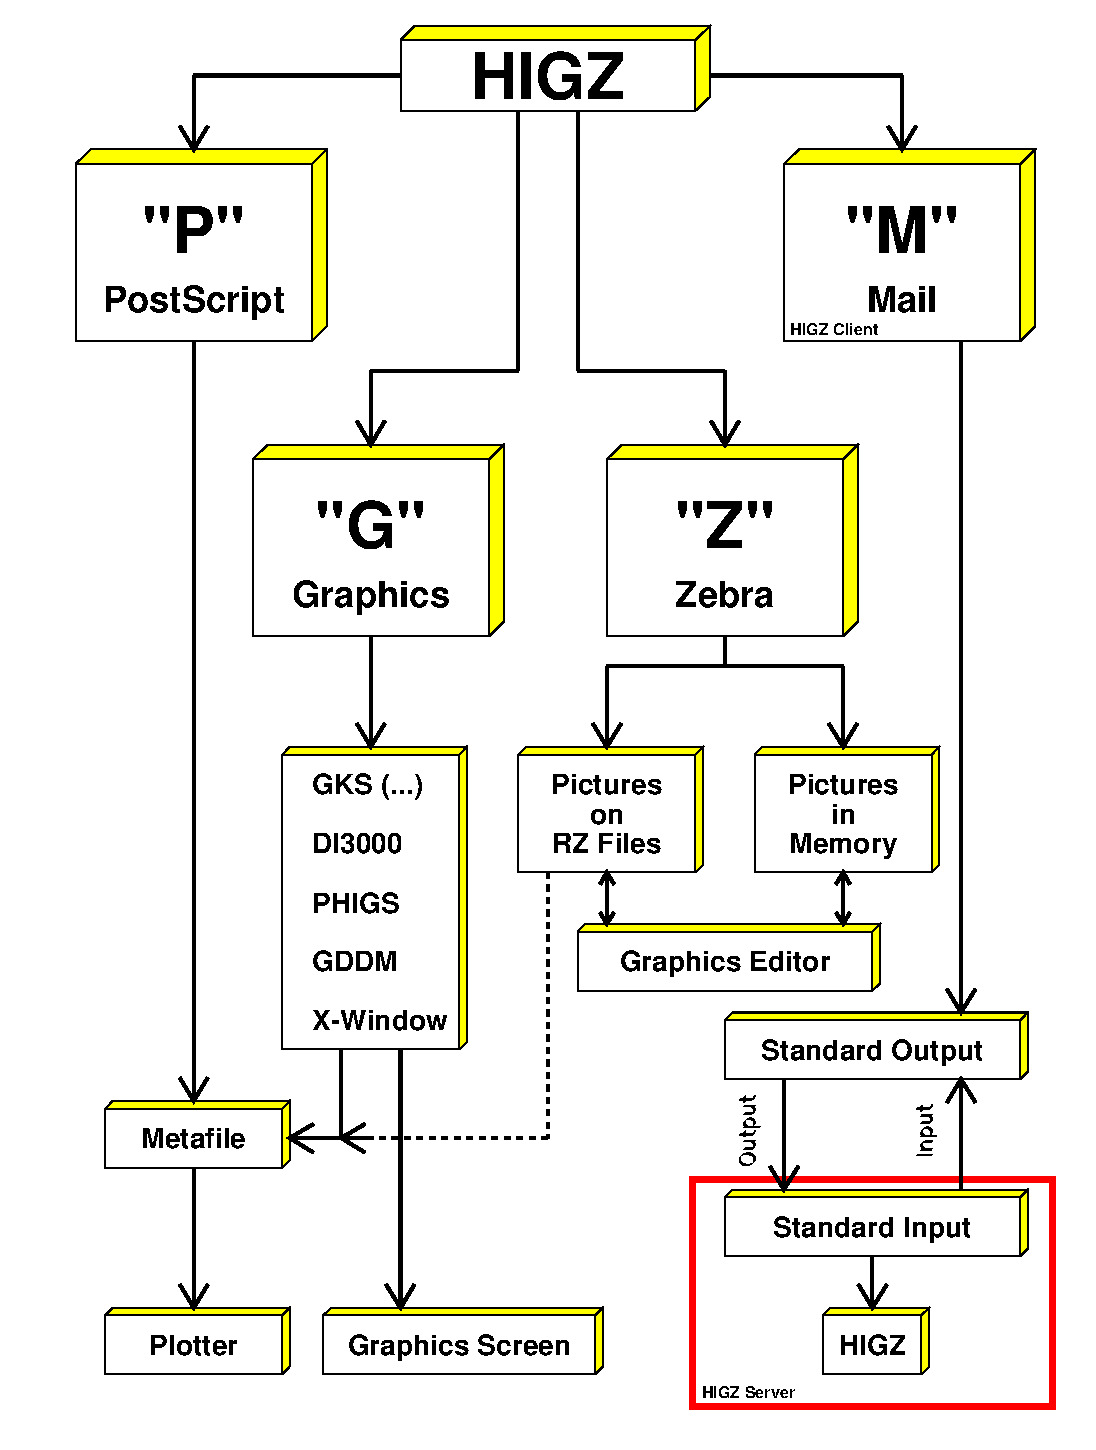
\epsfig{file=higzsys.eps,height=15cm}}\end{center}
\caption{Structure of the \HIGZ~system.}
\label{HIGZSYS}
\end{Fighere}
 

         % Introduction
%%%%%%%%%%%%%%%%%%%%%%%%%%%%%%%%%%%%%%%%%%%%%%%%%%%%%%%%%%%%%%%%%%%%%%%%%%%%%%%%
%                                                                              %
%   HIGZ  User Guide -- LaTeX Source                                           %
%                                                                              %
%   Chapter: Control routines                                                  %
%                                                                              %
%   This document needs the following external EPS files:                      %
%     none                                                                     %
%                                                                              %
%   Editor: Michel Goossens / AS-MI                                            %
%   Last Mod.: 9 July 1993 oc                                                  %
%                                                                              %
%%%%%%%%%%%%%%%%%%%%%%%%%%%%%%%%%%%%%%%%%%%%%%%%%%%%%%%%%%%%%%%%%%%%%%%%%%%%%%%%
\Filename{H1Overallcontrolroutines}
\chapter{Overall control routines}

\Filename{H2Controlroutines}
\section{Control routines}
\index{control!routines}
 
\subsection{Initialization}
\index{initialization}
\Shubr{IGINIT}{(NWHIGZ)}
\Action
This routine initializes \HIGZ. This must be the first function to be used in
the \HIGZ~package.
\Pdesc
\begin{DLtt}{1234567}
\item[NWHIGZ] Minimal \ZEBRA~dynamic space in memory for the \HIGZ~division;
              A value of 0, indicates that allocation will be done
	      automatically. {\tt NWHIGZ} must be less than {\tt NWORDS-5000}
              where {\tt NWORDS} is the size of the common block {\tt PAWC}
              (see below).
\end{DLtt}
The \ZEBRA~memory allocation must be defined in the application program with
the common block:
\begin{XMP}
      COMMON/PAWC/RPAW(NWORDS)
\end{XMP}
If \HIGZ~is used outside the context of \PAW~the routine \Rind{MZPAW} must be
called in the main program in order to initialize the \ZEBRA~package
\cite{bib-ZEBRA}, before calling \Rind{IGINIT}. Note that packages like
\HBOOK\cite{bib-HBOOK}, \HPLOT\cite{bib-HPLOT}, \PAW\cite{bib-PAW} and
\KUIP\cite{bib-KUIP} call \Rind{MZPAW} directly and therefore the user should
not issue such a call. These packages store dynamic structures in the same
common {\tt/PAWC/}.
\begin{XMP}
      CALL MZPAW(NWORDS,'M')
\end{XMP}
 
\subsection{Termination}
\index{termination}
\Shubr{IGEND}{ }
\Action
This routine terminates \HIGZ. This must be the last call to be issued in a
\HIGZ~session. \Rind{IGEND} deactivates and closes all open workstations.
It also closes the basic graphics package by calling \Rind{IDAWK}, \Rind{ICLWK},
\Rind{ICLKS}.
 
\subsection{Graphic package control}
\index{graphic!package!control}
\Shubr{IGSSE}{(IERRF,KWTYPE)}
\Action
In general, the initialization of the underlaying graphics package consists in
several calls to different routines, in order to set the environment parameters.
For user's convenience and for most applications, \Rind{IGSSE} initializes the
standard graphic package environment. In particular, the default primitives
attributes and the default window, viewport, workstation window and workstation
viewport are initialized. Sophisticated applications may need to call the
specialized basic control routines, namely \Rind{IOPKS}, \Rind{IOPWK},
\Rind{IACWK}, \Rind{ISWKWN} and \Rind{ISWKVP}, instead of using \Rind{IGSSE}.
\Rind{IGSSE} opens only a single workstation.
\Pdesc
\begin{DLtt}{1234567}
\item[IERRF] Error file logical unit number.
\item[KWTYPE] Workstation type. See the description of \Rind{IOPWK} section
\ref{IOPWK}.
\end{DLtt}
\par
\Rind{IGSSE} calls the following routines:
\begin{DLtt}{1234567890123456789012345}
\item[IOPKS] See section \ref{IOPKS}.
\item[IOPWK(1,KONID,KWTYPE)] See section \ref{IOPWK}.
\item[IACWK(1)] See section \ref{IACWK}.
\end{DLtt}
Note that {\tt KONID} is initialized in \Rind{IGSSE} depending on the \UGP~
used. In general {\tt KONID} is set to 1.
\par
The workstation window and viewport are also initialized in
\Rind{IGSSE} as follows:
\begin{XMP}
     CALL ISWKWN(1,0.,1.,0.,1.)
     CALL ISWKVP (1,0.,XMAX,0.,YMAX)
\end{XMP}
where {\tt XMAX} and {\tt YMAX} are the screen dimensions in pixels.
\par
The following primitives attributes are
initialized:
\index{polyline!colour index!default value}
\index{polyline!type!default value}
\index{polyline!width!default value}
\index{polymarker!colour index!default value}
\index{polymarker!type!default value}
\index{polymarker!scale factor!default value}
\index{fill area!colour index!default value}
\index{fill area!interior style!default value}
\index{fill area!style index!default value}
\index{text!character height!default value}
\index{text!character up vector!default value}
\index{text!alignment!default value}
\index{text!font and precision!default value}
\index{text!colour index!default value}
\index{clipping!default value}
\index{GKS@{{\sf GKS}}!aspect source flag}
\index{default attributes values}
 
\begin{center}
\begin{tabular}{||l|l||}
\hline
 Attributes names            & Default values         \\
\hline
Polyline colour index        & 1                      \\
Line type                    & 1                      \\
Line width                   & 1.0                    \\
Polymarker colour index      & 1                      \\
Marker type                  & 1                      \\
Marker scale factor          & 1.0                    \\
Fill area colour index       & 1                      \\
Fill area interior style     & 0                      \\
Fill area style index        & 1                      \\
Character height             & 0.01                   \\
Character up vector          & 0.0,1.0                \\
Text alignment               & 0,0                    \\
Text font and precision      & 0,2                    \\
Text colour index            & 1                      \\
Clipping indicator           & 1                      \\
\GKS~Aspect source flag      & Individual attributes  \\
\hline
\end{tabular}
\end{center}

\par
\index{colour table}
The first heigh elements of the colour table are initialized as follow:
\begin{center}
\begin{tabular}{||c|l||}
\hline
 Colour indeces              & Colour                 \\
\hline
            0                & White                  \\
            1                & Black                  \\
            2                & Red                    \\
            3                & Green                  \\
            4                & Blue                   \\
            5                & Yellow                 \\
            6                & Magenta                \\
            7                & Cyan                   \\
\hline
\end{tabular}
\end{center}
 
\index{telnetg}
In addition to this initialization role, \Rind{IGSSE}, when it is used in the
context of the \TELNETG~program, allows to open the connection between the
remote machine and the local one even if the \XW~is not available.
This is done by giving to \Rind{IGSSE} the negative value of the local
workstation type.
\subsection{Display control}
\index{display!control}
\par
Many terminals provide different modes: for example a Tektronix emulation mode
(or graphics mode) and a VT100 emulation mode (or alphanumeric mode). Some
terminals have (additionally) two overlayed screens: a graphics screen and an
alphanumeric screen (or dialog scroll). If a \FORTRAN~input is requested, the
operating system generally displays a prompt (for example ``{\tt CMS READ}''),
which belongs to the alphanumeric screen in VT100 emulation mode.
\index{alphanumeric mode}
\par
\HIGZ~provides two functions to switch between these modes and to enable
\FORTRAN~input and output. In some systems (e.g. IBM's VM/CMS) it is essential
that all \FORTRAN~input/output be performed in alphanumeric mode, else an
abend will occur.

\begin{minipage}[t]{.49\textwidth}
\subsubsection*{Graphic mode}
\index{graphic!mode}
\Shubr{IGSG}{(KWKID)}
\Action
This routine takes the terminal back into graphics mode and e\-na\-bles
gra\-phics in\-put/out\-put. This task is in general performed automatically by
all the basic graphics routines.
\Pdesc
\begin{DLtt}{1234567}
\item[KWKID] Workstation identifier
\end{DLtt}
\end{minipage}
\hfill
\begin{minipage}[t]{.49\textwidth} 
\subsubsection{Alphanumeric mode}
\index{alphanumeric mode}
\Shubr{IGSA}{(KWKID)}
\Action
This routine takes the terminal out of graphics mode into alphanumeric mode. On 
terminals like Pericom Graphics the bell is rung and the user has to press the 
{\tt <CR>} key to continue.
\Pdesc
\begin{DLtt}{1234567}
\item[KWKID] Workstation identifier
\end{DLtt}
\end{minipage}
 
\Filename{H2TheminimalHIGZprogram}
\section{The minimal \HIGZ~program}
We are now able to write the minimal \HIGZ~program which only opens and closes
\HIGZ~without doing any graphics. All the graphics routines described in the
rest of this manual will be placed between the call to \Rind{IGSSE} and the
call to \Rind{IGEND}.
\begin{XMPt}{The minimal \HIGZ~program}
      PROGRAM MINIMAL
*
      PARAMETER (NWPAW=20000)
      COMMON/PAWC/RPAW(NWPAW)
*                                Initialize storage in /PAWC/.
      CALL MZPAW(NWPAW,'M')
*                                Initialize \HIGZ.
      CALL IGINIT(0)
*                                Set standard environment.
*                                Errors are written to standard output (UNIT 6).
*                                Workstation type is 1.
      CALL IGSSE(6,1)
*                                Deactivate and close all open workstations 
*                                Close \HIGZ.
      CALL IGEND
*
      END
\end{XMPt}
Note that by default the \Rind{MZPAW} routine does a verbose initialization of
\ZEBRA. 
To have a quiet initialization the single call to \Rind{MZPAW} should be replaced by:

\begin{XMP}
      CALL MZEBRA(-3)
      CALL MZPAW(NWPAW,' ')
\end{XMP}

Warning: on the IBM VM/CMS systems, if \HIGZ~is used with the \X11~driver a: 

\begin{XMP}
      CALL INITC
\end{XMP}

is mandatory in the main program to force the loading of the C library.
\index{X11 driver on IBM VM!INITC}
         % Control sequence Routines
%%%%%%%%%%%%%%%%%%%%%%%%%%%%%%%%%%%%%%%%%%%%%%%%%%%%%%%%%%%%%%%%%%%%%%%%%%%%%%%%
%                                                                              %
%   HIGZ  User Guide -- LaTeX Source                                           %
%                                                                              %
%   Chapter: Basic graphics routines                                           %
%                                                                              %
%   This document needs the following external EPS files:                      %
%            higznwt.eps                                                       %
%            col8.eps                                                          %
%            fais.eps                                                          %
%            fasi.eps                                                          %
%            line.eps                                                          %
%            linew.eps                                                         %
%            marker.eps                                                        %
%            markersf.eps                                                      %
%            align.eps                                                         %
%            psex1.eps                                                         %
%            psex2.eps                                                         %
%            psfont.eps                                                        %
%            pstext1.eps                                                       %
%            pstext2.eps                                                       %
%                                                                              %
%   Editor: Olivier Couet / CN-AS                                              %
%   Last Mod.: 9 July 1993 oc                                                  %
%                                                                              %
%%%%%%%%%%%%%%%%%%%%%%%%%%%%%%%%%%%%%%%%%%%%%%%%%%%%%%%%%%%%%%%%%%%%%%%%%%%%%%%%
\Filename{H1Thebasicgraphicsroutines}
\chapter{The basic graphics routines}
\index{graphics!basic routines}
%
%              Control
%
\Filename{H2Control}
\section{Control}
\index{control}
%
\subsection{Graphic package open}
\index{graphic!package!open}
\Shubr[GKS]{IOPKS}{(IERRF)}
\Action
This routine initializes the graphic package for use. It should be the
first of all graphic package routines called by the user program, just after
the call to \Rind{IGINIT}. The opposite of \Rind{IOPKS} is \Rind{ICLKS}.
\par
This routine is called by \Rind{IGSSE} and it must {\bf NOT} be called if
\Rind{IGSSE} has been already invoked.
\Pdesc
\begin{DLtt}{1234567}
\item[IERRF] Logical unit number of the file for recording error messages.
             If {\tt IERRF} is equal to {\tt 6}, the error messages are printed
             on the screen otherwise they are redirected to the file
             {\tt higz.err} or to the error file opened by the \UGP.
\end{DLtt}
%
\subsection{Graphic package close}
\index{graphic!package!close}
\Shubr[GKS]{ICLKS}{ }
\Action
This routine terminates the usage of the graphic package. It is the opposite
of \Rind{IOPKS}. The routine \Rind{ICLKS} should be called only when there are
no open workstations (see routine \Rind{ICLWK}). Note that \Rind{IGEND}
calls \Rind{ICLKS} automatically.
%
\subsection{Workstation open}
\index{workstation!open}
\Shubr[GKS]{IOPWK}{(KWKID,KONID,KWTYPE)}
\Action
This routine initializes a workstation for use. It is usually the second
of all graphic package routines called by the user program.
Note that more than one workstation may be opened at the same time. A
workstation means a terminal, a graphics window, or a metafile (see section
\ref{IGMETA}). The opposite of \Rind{IOPWK} is \Rind{ICLWK}. Note that
\Rind{IGSSE} opens and activates the workstation number 1 (see section
\ref{IGSSE}), \Rind{IGMETA} use the workstation number 2 (see section
\ref{IGMETA}).
\Pdesc
\begin{DLtt}{1234567}
\item[KWKID] Workstation identifier. It must be used in subsequent calls
             to activate or deactivate the workstation (\Rind{IACWK} and
	     \Rind{IDAWK}), to clear it (\Rind{ICLRWK}), or to close it
	     (\Rind{ICLWK}). {\tt KWKID} is also used in certain inquiry or
	     option setting routines.
\item[KONID] Connection identifier. It is a system-specific identifier related
             to the access way to the graphics device. \HIGZ~doesn't use it
             and pass it directly to the \UGP. If the workstation to be
             opened is a metafile, {\tt KONID} is the logical unit number
             on which the \FORTRAN~file has been opened (see section
             \ref{IGMETA}) in this case it can be any number smaller than 100.
\item[KWTYPE] Workstation type. It selects which type of workstation has to be
              opened. {\tt KWTYPE} must be among the predefined types that are
              supported by the \UGP~(see the appendix B). With the \X11, \GPR,
	      and \GL~versions of \HIGZ~the {\tt KWTYPE} corresponds to a line
	      number in the file \HW~(or {\tt HIGZWIN DATA} on {\tt IBM/VM}
	      machines). When \Rind{IOPWK} is called, it tries to open the file
	      \HW~in the working directory. If it does not succeed it tries in
	      the HOME directory. If it doesn't succeed again it creates this
	      file in the home directory as follows:
\begin{verbatim}
                      0000 0000 0600 0600
                              .
                              .
                              .
                      0000 0000 0600 0600
\end{verbatim}
where the lines define each of the workstation types (from 1 to 10) with
the x-margin (left), y-margin (top), x-size (width) and y-size (height) of the
corresponding window in pixels.

Using the \X11~version the output is redirected (like for all \X11~applications)
to the display defined via the environment variable {\tt DISPLAY}.
\end{DLtt}
%
\subsection{Get workstation type}
\index{get!workstation type}
\Shubr{IGWKTY}{(KWTYPE*)}
\Action
This routine gets the workstation type from the standard input.
\Pdesc
\begin{DLtt}{1234567}
\item[KWTYPE] Workstation type. A call to this routine will prompt the user
              with:
\begin{verbatim}
Workstation type (?=HELP) <CR>=1
\end{verbatim}
Just typing {\tt CR} will return the default value in {\tt KWTYPE}. The value of
the default depends on the \HIGZ~installation. Typing {\tt ?} will give a short
help listing on all the different possible workstation types. Any other answer
will be interpreted as a new workstation type. Note that with the \X11~version
of \HIGZ{} the routine \Rind{IGWKTY} will accept a workstation type like:
{\tt n.hostname} where {\tt n} is the line number in the file \HW{} and
{\tt hostname} is the name of the machine on which the graphics will be
displayed. In this way it is not necessary to define the variable {\tt DISPLAY}
before using \HIGZ.

\begin{ULc}
\item   If a workstation type like {\tt n.hostname} is entered,
        the {\tt hostname} is written at the end of the line {\tt n} in \HW.
\item   If the workstation type {\tt n} is entered and if a {\tt hostname} is
        present on the line {\tt n} in \HW, the graphics will be redirected
        to the machine
        {\tt hostname}.
\item   If the workstation type {\tt n} is entered and if a {\tt hostname} is
        not on the line {\tt n} in \HW, the graphics  will be redirected
        to the ma\-chi\-ne de\-fi\-ned by the va\-ria\-ble {\tt DIS\-PLAY}.
\item   If the workstation type {\tt n.} is entered and if a {\tt hostname} is
        present on the line {\tt n} in \HW, the graphics  will be redirected
        to the machine defined by the variable {\tt DISPLAY} and {\tt hostname}
        is removed from the line {\tt n} in \HW.
\end{ULc}
\end{DLtt}
\Remark
In the file \HW, it is possible to specify the name of the window just after
the \Lit{hostname}.
%
\newpage
\subsection{Workstation close}
\index{workstation!close}
\Shubr[GKS]{ICLWK}{(KWKID)}
\Action
This routine terminates the usage of the workstation. It is the opposite of
\Rind{IOPWK}.
\Pdesc
\begin{DLtt}{1234567}
\item[KWKID] Workstation identifier defined in \Rind{IOPWK}.
\end{DLtt}
%
\subsection{Workstation activation}
\index{workstation!activation}
\Shubr[GKS]{IACWK}{(KWKID)}
\Action
This routine prepares a previously opened workstation (see routine \Rind{IOPWK})
to receive output primitives. It must always be used for workstations on which
one wishes to draw primitives. In addition, \Rind{IACWK} and its opposite
\Rind{IDAWK} are used with multiple workstations to control which of them will
receive any new primitives.
\Pdesc
\begin{DLtt}{1234567}
\item[KWKID] Workstation identifier defined in \Rind{IOPWK}.
\end{DLtt}
%
\subsection{Workstation deactivation}
\index{workstation!deactivation}
\Shubr[GKS]{IDAWK}{(KWKID)}
\Action
This routine deactivates an active workstation. It is the opposite of
\Rind{IACWK}. It must always be used before closing a workstation previously
activated. In addition, \Rind{IACWK} and \Rind{IDAWK} are used when multiple
workstations are open to control which of them receive any new primitives.
\Pdesc
\begin{DLtt}{1234567}
\item[KWKID] Workstation identifier.
\end{DLtt}
%
\subsection{Update workstation}
\index{workstation!update}
\index{flush graphics buffers}
\Shubr[GKS]{IUWK}{(KWKID,IRFLG)}
\Action
This routine updates the workstation KWKID. It send all buffered output to the
screen. In the \X11~version of \HIGZ, this routine allows to flush the
\X11~buffer. This routine is usually called with the first parameter equal to
0 and the second to 1.
\Pdesc
\begin{DLtt}{1234567}
\item[KWKID] Workstation identifier.
             \Lit{KWKID = 0} updates all the current open workstations.
\item[IRFLG] Regeneration flag:
\begin{DLtt}{12345}
\item[0] postpone update workstation (only when the \UGP~is \GKS)
\item[1] refresh entire display
\item[2] update current view
\end{DLtt}
\end{DLtt}
%
\newpage
\subsection{Update workstation and go to alphanumeric mode}
\index{flush graphics buffers}
\Shubr{IGTERM}{ }
\Action
Very often application programs require to update the open workstations and
then return to the alphanumeric mode. This routine without parameters,
provides these two actions. Essentially it performs the following calls:
\begin{verbatim}
CALL IUWK(0,1)
CALL IGSA(0)
\end{verbatim}
%
\subsection{Workstation clear}
\index{workstation!clear}
\Shubr[GKS]{ICLRWK}{(KWKID,KOFL)}
\Action
This routine clears the output area of a workstation which has been previously
opened.
\Pdesc
\begin{DLtt}{1234567}
\item[KWKID] Workstation identifier. On a softcopy device (e.g. a terminal), the
             output area is cleared. On a hardcopy device, the paper is
	     advanced, so that a fresh area is available for drawing. If
	     {\tt KWKID =0} then all active workstations are cleared.
\item[KOFL] Flag controlling the operation of routine \Rind{ICLRWK} on a
            workstation for which the output area is already cleared. Possible
	    values are:
\begin{DLtt}{123}
\item[0] If there has been no output since the previous \Rind{ICLRWK},
         nothing happens.
\item[1] The output medium is advanced or cleared in any cases.
\end{DLtt}
\end{DLtt}
If a change has been requested in the \WT~(via \Rind{ISWKVP} or \Rind{ISWKWN}),
the \WT~is recalculated when \Rind{ICLRWK} is called.

With the \GPR, \GL, and \X11~versions of \HIGZ, if the window size has changed,
the new size will be automatically taken into account after a clear workstation.
%
%              The coordinate systems and transformations
%
\Filename{H2coordinatesystem}
\section{The coordinate systems and transformations}
\index{coordinates!systems}
The coordinate systems and transformations are the same as for \GKS.
Three coordinate systems are used, namely the \WC~(\wc), \NDC~(\ndc) and
\DC~(\dc) systems. Two transformations are then necessary, the \NT~(\nt) going
from \WC~to \NDC~space and the \WT~(\wt) going from \NDC~to \DC~space.
\par
The \NDC~space is a fixed space, a square whose bottom left corner
(the origin) has the coordinates {\tt(0.,0.)} and the top right corner
has the coordinates {\tt(1.,1.)}.
\par
The mapping from \NDC~to \DC~and in general the knowledge of
device parameters is supplied by default by the standard initialization
function (but user callable routines are also provided).
The complete viewing pipeline is described on figure \ref{NTWT}.
\index{viewing pipeline}
\par
For devices with variable windowing capabilities, \HIGZ~gives the possibility
to change dynamically or after a clear (see \Rind{ICLRWK}) the device viewport,
and to inform the basic graphics package of this via the routine \Rind{IGQWK}
(see section \ref{IGQWK}).

\begin{figure}[p]
\begin{center}\mbox{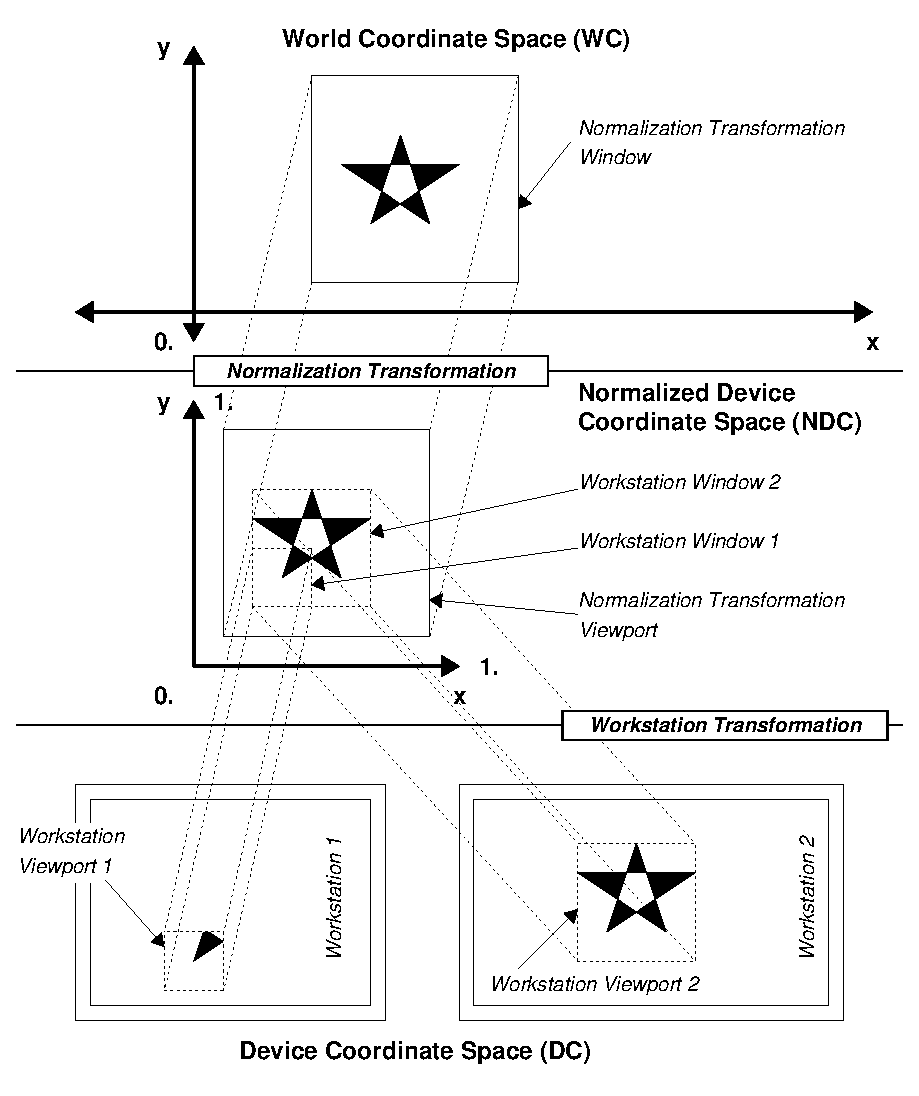
\epsfig{file=higznwt.eps,width=\the\textwidth}}\end{center}
\caption{Normalization and Workstation Transformations.}
\label{NTWT}
\end{figure}
\clearpage

\subsection{Workstation window definition}
\index{workstation!window definition}

\Shubr[GKS]{ISWKWN}{(KWKID,XMIN,XMAX,YMIN,YMAX)}
\Action
This routine defines a workstation window in the \NDC~space.
It sets the (requested) workstation window on a previously opened
workstation. The workstation window, specified in \NDC~
(i.e., {\tt0.-1.} by {\tt0.-1.}) is the portion of \NDC~space that the
application wishes to appear on the given workstation. This permits primitives
which are created when multiple workstations are active to be clipped and scaled
differently on the different workstations.

The workstation window (together with the workstation viewport and the rule that
the aspect ratio of the workstation window must be preserved) determines the
mapping (uniform scale with translation) from \NDC~to \DC.

The requested workstation window becomes the current workstation window either
during the invocation of \Rind{ISWKWN} (if the display surface is empty or if it
does not cause an implicit regeneration) or at some later time (for example,
during an invocation of \Rind{ICLRWK}).
\Pdesc
\begin{DLtt}{1234567}
\item[KWKID]Workstation identifier
\item[XMIN] X coordinate of the lower left hand corner in \ndc~space.
\item[XMAX] X coordinate of the upper right hand corner in \ndc~space.
\item[YMIN] Y coordinate of the lower left hand corner in \ndc~space.
\item[YMAX] Y coordinate of the upper right hand corner in \ndc~space.
\end{DLtt}
The four last parameters must be between {\tt0.0} and {\tt1.0}
(inclusive) and must satisfy {\tt XMIN < XMAX} and {\tt YMIN < YMAX}.
%
\subsection{Workstation viewport definition}
\index{workstation!viewport definition}
\Shubr[GKS]{ISWKVP}{(KWKID,XMIN,XMAX,YMIN,YMAX)}
\Action
This routine sets the (requested) workstation viewport on a previously opened
workstation. The workstation viewport, specified in \DC, is the
portion of the maximum available display surface that the application wishes to
use (see section \ref{IGQWK}).

The workstation viewport (together with the workstation window and the rule that
aspect ratios must be preserved) also determines the mapping (uniform scaling
with translation) from \NDC~to \DC.

The requested workstation viewport becomes the current workstation viewport
either during the invocation of \Rind{ISWKVP} (if the display surface is empty
or if it does not cause an implicit regeneration) or at some later time (for
example, during an invocation of \Rind{ICLRWK}). The \DC~region
specified by the parameters must be contained in  or equal to the maximum
available display  surface. The initial requested workstation viewport is the
entire display surface.
\Pdesc
\begin{DLtt}{1234567}
\item[KWKID]Workstation identifier
\item[XMIN] X coordinate of the lower left hand corner in \dc~space
\item[XMAX] X coordinate of the upper right hand corner in \dc~space
\item[YMIN] Y coordinate of the lower left hand corner in \dc~space
\item[YMAX] Y coordinate of the upper right hand corner in \dc~space
\end{DLtt}
The last four parameters must satisfy the conditions {\tt XMIN < XMAX} and
{\tt YMIN < YMAX}.
%
\subsection{Normalization Transformation window definition}
\index{normalization transformation!window definition}
\Shubr[GKS]{ISWN}{(NT,XMIN,XMAX,YMIN,YMAX)}
\Action
This routine sets the boundaries of the window of a \NT. The window must be
specified in \WC. The boundaries of the window, together with the
boundaries of the viewport (which are in \NDC)
determine a transformation from \WC~to \NDC~consisting of
separate X and Y scale factors and a translation in two dimensions. The \NT~is
selected by using routine \Rind{ISELNT}.
\Pdesc
\begin{DLtt}{1234567}
\item[NT]   Normalization transformation index ({\tt 0<NT<1000000}).
\item[XMIN] X coordinate of the lower left hand corner in \wc~space.
\item[XMAX] X coordinate of the upper right hand corner in \wc~space.
\item[YMIN] Y coordinate of the lower left hand corner in \wc~space.
\item[YMAX] Y coordinate of the upper right hand corner in \wc~space.
\end{DLtt}
The last four parameters must satisfy the conditions {\tt XMIN < XMAX} and
{\tt YMIN < YMAX}.
%
\subsection{Normalization Transformation viewport definition}
\index{normalization transformation!viewport definition}
\Shubr[GKS]{ISVP}{(NT,XMIN,XMAX,YMIN,YMAX)}
\Action
This routine sets the boundaries of the viewport of a \NT. The viewport must be
specified in \NDC. The boundaries of the viewport have
two roles:
\begin{OL}
\item Together with the boundaries of the window (which are in \WC)
      they determine a transformation from \WC~to \NDC~consisting of
      separate X and Y scale factors and a translation in two dimensions.
\item When the clipping indicator is 1 (see routine \Rind{ISCLIP}), primitives
      are clipped to the boundary of the viewport (once the primitives are
      transformed to \NDC)
\end{OL}
The \NT~is selected with the routine \Rind{ISELNT}.
\Pdesc
\begin{DLtt}{1234567}
\item[NT]   Normalization transformation index ({\tt 0<NT<1000000}).
\item[XMIN] X coordinate of the lower left hand corner in \dc~space
            ($0.0 \leq $\Lit{XMIN}$\leq 1.0$).
\item[XMAX] X coordinate of the upper right hand corner in \dc~space
            ($0.0 \leq $\Lit{XMAX}$\leq 1.0$).
\item[YMIN] Y coordinate of the lower left hand corner in \dc~space
            ($0.0 \leq $\Lit{YMIN}$\leq 1.0$).
\item[YMAX] Y coordinate of the upper right hand corner in \dc~space
            ($0.0 \leq $\Lit{YMAX}$\leq 1.0$).
\end{DLtt}
The last four parameters must satisfy the conditions {\tt XMIN < XMAX} and
{\tt YMIN < YMAX}.
%
\subsection{Normalization transformation selection}
\index{normalization transformation!selection}
\Shubr[GKS]{ISELNT}{(NT)}
\Action
This routine selects the \NT~to be used when \WC~must be mapped
to or from \NDC~(\ndc). These mappings usually take
place during invocations of primitives (\Rind{IFA}, \Rind{IPL}, \Rind{IPM}, and
\Rind{ITX}) and during graphics input (\Rind{IRQLC}).

Transformation {\tt0} always has a window and a viewport that are the unit
square ({\tt0.-1.} by {\tt0.-1.}) and cannot be changed with \Rind{ISVP} or
\Rind{ISWN}. Transformation {\tt0} is selected by default.
\Pdesc
\begin{DLtt}{1234567}
\item[NT] Normalization transformation index ({\tt 0<NT<1000000}). The number of transformations is
          limited to 50.
\end{DLtt}
%
\subsection{Simplified way to define the viewing pipeline}
\index{viewing pipeline}
Very often the user of a graphics package wants to define the dimensions of
the physical output in centimeters and centered on the output devices (screen or
paper). This can be done with \HIGZ~with simply one call to the routine
\Rind{IGRNG}.
\Shubr{IGRNG}{(XSIZE,YSIZE)}
\Action
\index{centimeter!conversion to \NDC}
This routine is used to determine the physical dimensions (in centimeter)
and to optimize the aspect ratio and the centering of a picture.
If the {\tt X} or {\tt Y} dimension of output device are smaller than
{\tt XSIZE} or {\tt YSIZE}, a scaling factor is applied to the final size
of the picture but the aspect ratio is kept.
When an \EPS~workstation is active, a call to this routine is mandatory
in order to define the size of the picture (e.g the \PS~{\sf BoundingBox}).
\index{PostScript!Encapsulated!BoundingBox}
\Pdesc
\begin{DLtt}{1234567}
\item[XSIZE] Picture size in centimeters in the X direction.
\item[YSIZE] Picture size in centimeters in the Y direction.
\end{DLtt}
\par
After a call to \Rind{IGRNG} the \NT~number 1 is selected. For this reason
in all the \HIGZ~routines, the \NT~number {\tt 1} is assumed to be a centimeter
transformation. It is not recommended to define this transformation (via
\Rind{ISWN}, \Rind{ISVP} and \Rind{ISELNT}) outside \Rind{IGRNG}. In particular
when \PS~files are used, the \PS~driver assumes that the setting of the
\NT~{\tt 1} has been done via \Rind{IGRNG}.

After a call to \Rind{IGRNG} some useful value to convert centimeters into
\NDC{}, are available in the common \QUEST.
\begin{DLtt}{12345678901}
\item[RQUEST(11)] Ratio to convert cm into \NDC.
\item[RQUEST(12)] left position of the  \NT{} 1 viewport in \NDC.
\item[RQUEST(13)] bottom position of the \NT{} 1 viewport in \NDC.
\item[RQUEST(14)] width of the \NT{} 1 viewport in \NDC.
\item[RQUEST(15)] height of the \NT{} 1 viewport in \NDC.
\end{DLtt}
For more details, see examples on pages \pageref{HIEX1} and \pageref{HIEX4}.

\index{workstation!viewport definition}
\index{workstation!window definition}
%
%              Metafile control and printing
%
\Filename{H2Metafilecontrol}
\section{Metafile control and printing}
\index{metafile!control}
\index{printing}
A special \ASCII~file called metafile is needed in order to produce pictures
on paper. The metafiles are managed via all workstation control routines
previously described. The general sequence of actions to use metafiles is:
\begin{verbatim}
- Open a FORTRAN file
- Open a workstation (IOPWK) with the type metafile
- Activate the workstation
- Produce some graphics
- Deactivate the workstation
- Close the workstation
\end{verbatim}
%
\subsection{Simplified metafile control}
The routine \Rind{IGMETA} is provided in order to minimize the number of
calls to specialized \HIGZ~workstation control routines and to improve
the portability of applications. This routine opens, activates, deactivates
or closes a metafile.

\Shubr{IGMETA}{(LUN,KWTYPE)}
\Action
This routine permits the selection of a metafile, offering a choice of graphic
output to the screen and/or a metafile.
\Pdesc
\begin{DLtt}{1234567}
\item[LUN] Metafile logical unit number
\begin{DLtt}{1234567}
\item[LUN>0] The subsequent graphic output will be directed to both screen and
             metafile.
\item[LUN<0] The subsequent graphic output will be directed to the metafile
             only.
\item[LUN=0] Any previously open metafile is deactivated, and further graphic
             output will be directed to the screen only.
\item[LUN=999] Any previously open metafile is deactivated and closed, and
               further graphic output will be directed to the screen only.
               \PS~metafiles need to be closed in order to be printed.
\end{DLtt}
\item[KWTYPE] Workstation type. If {\tt KWTYPE = 0}, then \Rind{IGMETA} selects
              automatically the default workstation type. This defaults
              workstations depend on the \UGP~used (e.g. -111 for
	      \HIGZ/\X11 or 4 for \GKSGRAL).
\end{DLtt}
%
\subsection{\PS~metafile type}
\index{metafile!PostScript}
In addition to the metafile type provided by the underlaying graphics
package (for example 4 with \GKSGRAL), \PS~workstation types
are also available independently from the \UGP~used allowing generation of
high quality outputs. The \PS~workstation types have the following format:
\begin{verbatim}
                               -[Format][Nx][Ny][Type]
\end{verbatim}
    Where:
\begin{DLtt}{1234567}
\item[Format] Is an integer between 0 and 99 which defines the format of the
              paper. For example if {\tt Format}=3 the paper is in the standard
	      A3 format. {\tt Format}=4 and {\tt Format}=0 are the same and
	      define an A4 page. The A0 format is selected by {\tt Format}=99.
              The US format Letter is selected by {\tt Format}=100.
              The US format Legal is selected by {\tt Format}=200.
              The US format Ledger is selected by {\tt Format}=300.
\item[Nx, Ny] Specify respectively the number of zones on the x and y axis.
              {\tt Nx} and {\tt Ny} are integers between 1 and 9.
\item[Type] Can be equal to:
\begin{DLtt}{12}
\item[1] Portrait mode with a small margin at the bottom of the page.
\item[2] Landscape mode with a small margin at the bottom of the page.
\item[4] Portrait mode with a large margin at the bottom of the page.
\item[5] Landscape mode with a large margin at the bottom of the page.

         The large
         margin is useful for some \PS~printers (very often for the colour
         printers) \index{PostScript!colour printers} as they need more space to
	 grip the paper for mechanical reasons.

         Note that some \PS~colour
	 printers can also use the so called "special A4" format permitting
	 the full usage of the A4 area; \index{PostScript!special A4} in this
	 case larger margins are not necessary and {\tt Type}=1 or 2
         can be used.
\item[3] \EPS. This {\tt Type} permits the generation of files which can be
         included in other documents, for example \index{latex@\LaTeX{}!PostScript}
         in \LaTeX{} files. Note that with this {\tt Type}, {\tt Nx} and
	 {\tt Ny} must always be equal to 1, and {\tt Format} has no meaning.
	 The size of the picture must be specified by the user via the
	 \Rind{IGRNG} routine. Therefore the workstation type for \EPS~is -113.
	 For example if the name of an \EPS~file is {\tt example.eps}, the
	 inclusion of this file into a \LaTeX{} file will be possible via
	 (in the \LaTeX{} file):
\begin{verbatim}
   \begin{figure}
   \epsffile{example.eps}
   \caption{Example of Encapsulated PostScript in LaTeX.}
   \label{EXAMPLE}
   \end{figure}
\end{verbatim}
Note that all the figures in this manual are included in this way.
\end{DLtt}
\end{DLtt}
With {\tt Type=1,2,4} and 5 the pictures are centered on the page, and the
usable area on paper is proportional to the dimensions of A4 format.
\par
Examples:
\par
\Lit{-111} or \Lit{-4111} defines an A4 page not divided.
\Lit{-6322} define an A6 landscape page divided in 3 columns and 2 rows.
\begin{center}
\extrarowheight=1mm
\begin{tabular}{|*{3}{>{\quad}c<{\quad}|}}
\hline
1 & 2 & 3 \\ \hline
4 & 5 & 6 \\ \hline
\end{tabular}
\end{center}
The first picture  will be drawn  in the area 1. If the program clears the
screen via \Rind{ICLRWK}, the graphics output will appear in  the next area in
the order defined above. If a  page is filled, a new  page is used with
the same grid. Note that empty  pages are not printed  in order to save
paper.
\par
Ignoring  formats smaller  than A12, the total number of possible different
\PS~workstation types is: $4\times9\times9\times13+1 = 4213$ !

\subsection{Usage of \PS~metafiles in an user application program}
This section gives three examples showing the different ways of managing
\PS~files. The first example is the more general way, using
\Rind{IOPWK}, \Rind{IACWK} and \Rind{IGQWK} (see section \ref{IGQWK}). The
second example shows how to use the \Rind{IGMETA} routine. The last example
use \Rind{IGRNG} and \Rind{IGMETA}.
\begin{XMPt}{Example 1 : \Rind{IOPWK}, \Rind{IACWK} and \Rind{IGQWK}}

      DIMENSION R(2)
*
*              Open a \FORTRAN file
*
      OPEN(UNIT=10,FILE='test1.ps',FORM='FORMATTED',STATUS='UNKNOWN')
*
*              Open and activate a workstation with the \PS metafile
*              type -111 and with the workstation ID 5.
*              Note that the UNIT used to open the \FORTRAN (here 10)
*              is given as second parameter.
*
      CALL IOPWK(5,10,-111)
      CALL IACWK(5)
*
*              Get the size of the available space on paper. This is
*              now possible because the Format is known.
*
      CALL IGQWK(5,'MXDS',R)
*
*              Compute the size of the viewport according to the paper
*              size. Note that if the screen has not the same RATIO the
*              picture on screen and on paper will be different. In this
*              case the user must inquire the screen size and compute
*              a new viewport with this size and redraw on the screen
*              with the metafile deactivated.
*
      XV=R(1)/R(2)/2.
      YV=XV
      CALL ISVP(2,0.,XV,0.,YV)
      CALL ISWN(2,X1,X2,Y1,Y2)
      CALL ISELNT(2)
          .
          .
        Drawing
          .
          .
*
*              Deactivate and close the metafile
*
      CALL IDAWK(5)
      CALL ICLWK(5)
      CLOSE(10)

\end{XMPt}
\begin{XMPt}{Example 2 : \Rind{IGMETA}}

      DIMENSION R(2)
      OPEN(UNIT=10,FILE='test2.ps',FORM='FORMATTED',STATUS='UNKNOWN')
*
*              IGMETA permits the opening and activating of the metafile
*
      CALL IGMETA(10,-111)
      CALL IGQWK(2,'MXDS',R)
      XV=MIN(1.,R(1)/R(2))
      YV=MIN(1.,R(2)/R(1))
      CALL ISVP(2,0.,XV,0.,YV)
      CALL ISWN(2,X1,X2,Y1,Y2)
      CALL ISELNT(2)
          .
          .
        Drawing
          .
          .
*
*              Deactivate the metafile
*
      CALL IGMETA(0,0)
*
*              Close the metafile
*
      CALL ICLWK(2)
      CLOSE(10)

\end{XMPt}
\begin{XMPt}{Example 3 : \Rind{IGRNG}}

      DIMENSION R(2)
      OPEN(UNIT=10,FILE='test4.ps',FORM='FORMATTED',STATUS='UNKNOWN')
      CALL IGMETA(-10,-111)
*
*              IGRNG defines a size in cm centered on the page.
*              Even if the RATIO of the screen and the RATIO of
*              the paper are not the same the picture will appear
*              exactly the same on both.
*              Note that in the case of \EPS~(-113)
*              a call to IGRNG is mandatory.
*
      CALL IGRNG(10.,10.)
          .
          .
        Drawing
          .
          .
      CALL IGMETA(0,0)
      CALL ICLWK(2)
      CLOSE(10)
\end{XMPt}
\subsection{\LaTeX{} metafile type}
\index{metafile!\LaTeX{}}
\index{latex@\LaTeX{}}
\HIGZ~is able to produce metafiles which are ready to be included in \LaTeX{}
documents. These metafiles make use of the \verb'\picture' environment.
Compared to other possibilities of merging graphics
into documents, \LaTeX{} metafiles have a number of advantages:

\begin{ULc}
\item  The {\tt dvi} file is fully transportable as \verb'\special' commands are
       not used. This file can be output on any device for which a driver
       exists. Documents can be written, formatted, and previewed on
       workstations while the {\tt dvi} file can be sent via the  network to a
       central server for printing.
\item  The metafile can be also merged into the \LaTeX{} file to keep
       the full document in a single file.
\item  The power of \LaTeX{} in text processing can be used in the primitive
       \Rind{ITX} for example to generate complicated mathematical formulae
       on a document.
\end{ULc}

\subsubsection{\LaTeX{} metafile capabilities}

The capabilities of the \verb'\picture' environment are basically limited to
drawing straight horizontal or vertical lines. Slanted lines do exist but only
in a limited number of slopes and a minimum length of $\approx 4 {\rm mm}$.
Therefore slanted lines have to be approximated by small steps of straight lines
where the step size should be close to the printer resolution.
\par
The workstation type for \LaTeX{} metafiles is -777 for embedded files or
-778 for stand-alone files. Coordinates written to the metafile are integer
numbers assuming a grid spacing of $0.1 {\rm mm}$. Therefore the settings for
{\tt XSIZE} and {\tt YSIZE} should approximately correspond to the final
picture size.

\subsubsection{Line and marker types}

Line types 1 through 4 and marker types 1 through 5 are supported.

\subsubsection{Text fonts}

In addition to the software characters the font numbers -1 through -8 at
precision 0 can
be used. They map to the \TeX{} fonts {\rm Roman}, {\em Emphatic}, {\bf Bold},
{\it Italic}, {\sl Slanted}, {\sf Sans Serif}, {\sc Small Caps}, and
{\tt Typewriter}, respectively.
\par
\TeX{} fonts look much nicer and are faster to generate than software
characters generated by \Rind{IGTEXT}, but the disadvantage is that they are
available in horizontal orientation only and the character size does not scale
with the picture size.
\par
When using \TeX{} fonts the \Rind{IGTEXT} control characters
``\verb'<>[]"#^?!''' are interpreted to obtain superscripts, greek letters, and
other special characters. If a text string contains a ``\verb'\''' or
``\verb'{''' the remaining part is written verbatim into the metafile.
This allows to use \TeX{} formatting commands for elaborate displays.
Of course ``\verb'{''' and ``\verb'}''' must be properly matched.
\par
The whole text is typeset in math mode which does not allow a change of
fontsize in between. In order to format a formula on a larger size the formula
text must be preceded by ``\verb'{}$\large$'''.
\par
%\subsubsection{Example}
%\begin{figure}
%% HIGZ version 1.13/06 LaTeX metafile created  91/11/04   12.46
\ifx\higzunit\undefined\unitlength=0pt{}\else\unitlength=\higzunit\fi\ifdim\unitlength=0pt\unitlength=\textwidth\divide\unitlength
 2000\fi\par\noindent\begin{picture}(2000,2000)(0,0)\ifx\higzdraft\undefined\newcount\higzdraft\higzdraft=0{}\fi\ifnum\higzdraft>0
\put(0,0){\framebox(2000,2000){}}\else\ifx\higzstep\undefined\newcount\higzstep\higzstep=0{}\fi\ifnum\higzstep<1\higzstep=2
\fi\ifx\higzxx\undefined\newcount\higzxx\newcount\higzyy\newcount\higzx\newcount\higzy\newcount\higzdx\newcount\higzdy
\newcount\higzlx\newcount\higzly\newcount\higzslope\newcount\higzlen\newcount\higzllen\newcount\higzoffs\newcount\higzloffs
\newcount\higzadash\newcount\higzbdash\newcount\higzcdash\newcount\higzddash\newcount\higzmsize\newcount\higztemp\fi
\def\higzstroke#1,#2,#3,#4;{\advance\higzloffs\higzllen\ifnum\higzloffs>#1\advance\higzloffs-\higzllen\advance\higzloffs-#1
\higzloffs=-\higzloffs\ifnum#2>0\put(\higzlx,\higzly){\line(#3,#4){\higzloffs}}\fi\ifnum#2<0\put(\higzlx,\higzly){\circle*{0}}\fi
\higztemp=\higzloffs\multiply\higztemp#3\advance\higzlx\higztemp\higztemp=\higzloffs\multiply\higztemp#4\advance\higzly\higztemp
\advance\higzllen-\higzloffs\higzloffs=#1\else\ifnum#2>0\put(\higzlx,\higzly){\line(#3,#4){\higzllen}}\fi\ifnum#2<0\put(
\higzlx,\higzly){\circle*{0}}\fi\higzllen=0\fi}\def\higzdashed#1,#2,#3,#4,#5;{{\higzlx=#1\higzly=#2\higzllen=#5\higzloffs=
\higzoffs\loop\ifnum\higzloffs<\higzadash\ifnum\higzadash>1\higzstroke\higzadash,1,#3,#4;\else\higzstroke\higzadash,-1,#3,#4;\fi
\else\ifnum\higzloffs<\higzbdash\higzstroke\higzbdash,0,#3,#4;\else\ifnum\higzloffs<\higzcdash\higztemp=\higzcdash\advance
\higztemp-\higzbdash\ifnum\higztemp>1\higzstroke\higzcdash,1,#3,#4;\else\higzstroke\higzcdash,-1,#3,#4;\fi\else\ifnum\higzloffs<
\higzddash\higzstroke\higzddash,0,#3,#4;\else\higzloffs=0\fi\fi\fi\fi\ifnum\higzllen>0\repeat\global\higzoffs=\higzloffs}}\def
\higzsolid#1,#2,#3,#4,#5;{\put(#1,#2){\line(#3,#4){#5}}}\def\higzhslant#1,#2,#3;{\higzslope=#1\multiply\higzslope1000\advance
\higzslope500\divide\higzslope#2\higzlen=\higzslope\multiply\higzlen\higzstep\divide\higzlen1000\higzdy=0\loop\ifnum
\higzdy<#2\higzx=\higzxx\higzy=\higzyy\higzdx=\higzslope\multiply\higzdx\higzdy\advance\higzdx500\divide\higzdx1000\advance
\higzy\higzdy\multiply\higzdx#3\advance\higzx\higzdx\multiply\higzdx#3\advance\higzdx\higzlen\ifnum\higzdx>#1\advance
\higzlen#1\advance\higzlen-\higzdx\fi\higzline\higzx,\higzy,#3,0,\higzlen;\advance\higzdy\higzstep\repeat}\def\higzvslant#1,#2,#3;{
\higzslope=#2\multiply\higzslope1000\advance\higzslope500\divide\higzslope#1\higzlen=\higzslope\multiply\higzlen\higzstep
\divide\higzlen1000\higzdx=0\loop\ifnum\higzdx<#1\higzx=\higzxx\higzy=\higzyy\higzdy=\higzslope\multiply\higzdy\higzdx\advance
\higzdy500\divide\higzdy1000\advance\higzx\higzdx\multiply\higzdy#3\advance\higzy\higzdy\multiply\higzdy#3\advance
\higzdy\higzlen\ifnum\higzdy>#2\advance\higzlen#2\advance\higzlen-\higzdy\fi\higzline\higzx,\higzy,0,#3,\higzlen;\advance\higzdx
\higzstep\repeat}\def\s#1,#2;{\higzdx=#1{}\ifnum\higzdx<0\higzdx=-\higzdx\fi\higzdy=#2{}\ifnum\higzdy<0\higzdy=-\higzdy\fi\ifnum
\higzdx<\higzdy\ifnum#1<0\advance\higzxx#1\advance\higzyy#2\ifnum#2<0\higzvslant-#1,-#2,1;\else\higzvslant-#1,#2,-1;
\fi\else\ifnum#2<0\higzvslant#1,-#2,-1;\else\higzvslant#1,#2,1;\fi\advance\higzxx#1\advance\higzyy#2\fi\else\ifnum#2<0
\advance\higzxx#1\advance\higzyy#2\ifnum#1<0\higzhslant-#1,-#2,1;\else\higzhslant#1,-#2,-1;\fi\else\ifnum#1<0
\higzhslant-#1,#2,-1;\else\higzhslant#1,#2,1;\fi\advance\higzxx#1\advance\higzyy#2\fi\fi}\def\h#1;{\higzline\higzxx,
\higzyy,1,0,#1;\advance\higzxx#1}\def\r#1;{\higzline\higzxx,\higzyy,-1,0,#1;\advance\higzxx-#1}\def\U#1;{\higzline\higzxx,
\higzyy,0,1,#1;\advance\higzyy#1}\def\D#1;{\higzline\higzxx,\higzyy,0,-1,#1;\advance\higzyy-#1}\def\m#1,#2;{\higzxx=#1
\higzyy=#2}\def\higzdot#1,#2;{\put(#1,#2){\circle*{\higzmsize}}}\def\higzplus#1,#2;{\higzx=#1\multiply\higzx2\advance\higzx-
\higzmsize\divide\higzx2\put(\higzx,#2){\line(1,0){\higzmsize}}\higzy=#2\multiply\higzy2\advance\higzy-\higzmsize\divide
\higzy2\put(#1,\higzy){\line(0,1){\higzmsize}}}\def\higzstar#1,#2;{\higzplus#1,#2;\higzcross#1,#2;}\def
\higzcircle#1,#2;{\put(#1,#2){\circle{\higzmsize}}}\def\higzcross#1,#2;{\let\higzsave\higzline\let\higzline\higzsolid\higzlx=#1
\multiply\higzlx2\advance\higzlx-\higzmsize\divide\higzlx2\higzly=#2\multiply\higzly2\advance\higzly-\higzmsize\divide
\higzly2\m\higzlx,\higzly;\s\higzmsize,\higzmsize;\higzly=#2\multiply\higzly2\advance\higzly\higzmsize\divide\higzly2\m\higzlx,
\higzly;\s\higzmsize,-\higzmsize;\let\higzline\higzsave}\def\p#1,#2;{\higzmarker#1,#2;}\def\f#1,#2;{\put(\higzxx,
\higzyy){\makebox(#1,#2)[lb]{\rule{#1\unitlength}{#2\unitlength}}}}
% End of Initialisation
\let\higzline=\higzsolid\put(0,0){\framebox(2268,2268){}}\put(227,227){\framebox(1814,1814){}}\put(2211,2177){\makebox(0,0)[br]
{$\sf{}91/11/04\ {}\ {}\ {}12.46$}}
\fi\end{picture}

%\end{figure}

\subsubsection{Configuration parameters}
To some extent, the appearance of a picture can be changed at formatting time
by defining configuration parameters (in the \LaTeX{} file) which have the
following default values:
\begin{verbatim}
\newdimen\higzunit \higzunit=0pt
\newcount\higzstep \higzstep=2
\newcount\higzdraft \higzdraft=0
\end{verbatim}
\par
\index{higzunit}
By default the picture is automatically scaled to fill the full page width.
The picture size can be changed by setting \verb'\higzunit' to the wanted grid
spacing, e.g. to get the true {\tt XSIZE}:
\begin{verbatim}
\newdimen\higzunit \higzunit=0.1mm
\end{verbatim}
\par
\index{higzstep}
Slanted lines are approximated by straight lines along the major axis.
The step size along the minor axis is
\verb'\higzstep'$\times$\verb'\unitlength'.
By setting \verb'\higzstep=1' curves will look smoother
but if line segments come too close to the printer resolution the
{\tt dvi} driver may choose not to display them.
A larger value will result in faster formatting requiring less \TeX{} memory.
\par
\index{higzdraft}
Setting \verb'\higzdraft=1' replaces the actual picture by an empty box
of the same size to save formatting time during drafting.
%
\Filename{H2STARTFINISH}
\section{Examples: the routines {\tt START} and {\tt FINISH}}
The two routines used to produce the figures appearing this manual are
described in this section. They are good examples of a simple, but frequent,
usage of \HIGZ.

The first one: {\tt START}, initializes \HIGZ, opens an \EPS~file and set the
size of the figure according to the input parameters.

The second one: {\tt FINISH}, closes the \EPS~file and terminates \HIGZ.

\begin{XMPt}{The routine {\tt START}}
      SUBROUTINE START(NAME,X,Y)
      CHARACTER*(*) NAME
      PARAMETER (NWORDS=50000)
      COMMON /PAWC/ RPAW(NWORDS)
      CALL MZEBRA(-3)
      CALL MZPAW(NWORDS,' ')
      CALL IGINIT(0)
      CALL IGWKTY(ITYPE)
      CALL IGSSE(6,ITYPE)
      OPEN(UNIT=10,FILE=NAME//'.EPS',FORM='FORMATTED',STATUS='UNKNOWN')
      CALL IGMETA(10,-113)
      CALL IGRNG(X,Y)
      END
\end{XMPt}
In the routine {\tt FINISH} the call to the routine {\tt IGTERM} is not
mandatory but is useful to flush the graphics buffer especially in the
case of the \X11~interface (see section \ref{IGTERM}).
\begin{XMPt}{The routine {\tt FINISH}}
      SUBROUTINE FINISH
      CALL IGMETA(0,0)
      CALL ICLWK(2)
      CLOSE(10)
      CALL IGTERM
      CALL IGEND
      END
\end{XMPt}
\newpage
%
%              The basic output primitives
%
\Filename{H2Thebasicoutputprimitives}
\section{The basic output primitives}
\index{primitives}
\par
In \HIGZ~there are four basic output primitives: the polyline (\Rind{IPL}),
the fill area (\Rind{IFA}), the polymarker (\Rind{IPM}) and the text
(\Rind{ITX}). In all routines described in this section the coordinates
are given in the \WC~system.


\subsection{Polyline}
\index{primitives!polyline}
\index{polyline!drawing}
\Shubr[GKS]{IPL}{(N,X,Y)}
\Action
This routine draws a polyline on the currently active workstations (there must
be at least one). The polyline connects {\tt N} points ({\tt N$\geq$2}) by means
of {\tt N-1} line segments. The {\tt X} and {\tt Y} coordinates of the points
are in two {\tt N}-dimensional arrays.

The appearance of a polyline is controlled by the current ``polyline colour
index'' (see routine \Rind{ISPLCI} section \ref{ISPLCI}), the current
``line type'' (see routine \Rind{ISLN} section \ref{ISLN}) and the current
``line width'' (see routine \Rind{ISLWSC} section \ref{ISLWSC}).
\Pdesc
\begin{DLtt}{1234567}
\item[N] Number of points.
\item[X] Array of dimension {\tt N} containing the x coordinates in \wc~space.
\item[Y] Array of dimension {\tt N} containing the y coordinates in \wc~space.
\end{DLtt}


\subsection{Multiline}
\index{primitives!Multiline}
\index{Multiline!drawing}
\Shubr{IML}{(N,X,Y)}
\Action
This routine draws a multiline on the currently active workstations (there must
be at least one). The multiline connects \Lit{N} points ({\tt N$\geq$2}) two
by two. The \Lit{X} and \Lit{Y} coordinates of the points are in two 
\Lit{N}-dimensional arrays.

The appearance of a multiline is controlled by the current ``polyline colour
index'' (see routine \Rind{ISPLCI} section \ref{ISPLCI}), the current
``line type'' (see routine \Rind{ISLN} section \ref{ISLN}) and the current
``line width'' (see routine \Rind{ISLWSC} section \ref{ISLWSC}).
\Pdesc
\begin{DLtt}{1234567}
\item[N] Number of points.
\item[X] Array of dimension {\tt N} containing the x coordinates in \wc~space.
\item[Y] Array of dimension {\tt N} containing the y coordinates in \wc~space.
\end{DLtt}


\subsection{Polymarker}
\index{primitives!polymarker}
\index{polymarker!drawing}
\Shubr[GKS]{IPM}{(N,X,Y)}
\Action
This routine draws a polymarker on the currently active workstations (there must
be at least one). Markers are placed at {\tt N} points ({\tt N$\geq$1}), whose x
and y coordinates are given in two {\tt N}-dimensional arrays.

The appearance of a polymarker is controlled by the current ``polymarker colour
index'' (see routine \Rind{ISPMCI} section \ref{ISPMCI}), the current ``marker
type'' (see routine \Rind{ISMK} section \ref{ISMK}) and the current ``marker
scale factor'' (see routine \Rind{ISMKSC} section \ref{ISMKSC}).
\Pdesc
\begin{DLtt}{1234567}
\item[N] Number of points.
\item[X] Array of dimension {\tt N} containing the x coordinates in \wc~space.
\item[Y] Array of dimension {\tt N} containing the y coordinates in \wc~space.
\end{DLtt}


\subsection{Fill area}
\index{primitives!fill area}
\index{fill area!drawing}
\Shubr[GKS]{IFA}{(N,X,Y)}
\Action
This routine draws a filled area on the currently active workstations (there
must be at least one). The ``perimeter'' of the filled area has {\tt N} points
({\tt N$\geq$3}) whose x and y coordinates are given in two {\tt N}-dimensional
arrays.

The appearance of a filled area is controlled by the current ``filled area
colour index'' (see routine \Rind{ISFACI} section \ref{ISFACI}), the current
``filled area interior style'' (see routine \Rind{ISFAIS} section \ref{ISFAIS})
and the current ``filled area style index'' (see routine \Rind{ISFASI} section
\ref{ISFAIS}).
\Pdesc
\begin{DLtt}{1234567}
\item[N] Number of points.
\item[X] Array of dimension {\tt N} containing the x coordinates in \wc~space.
\item[Y] Array of dimension {\tt N} containing the y coordinates in \wc~space.
\end{DLtt}
%
\subsection{Text}
\index{primitives!text}
\index{text!drawing}
\Shubr[GKS]{ITX}{(X,Y,CHARS)}
\Action
This routine draws a text string on the currently active workstations
(there must be at least one).

The appearance of the text is controlled by attributes set by the current ``text
colour index'' (see routine \Rind{ISTXCI} section \ref{ISTXCI}), the current
``character height'' (see routine \Rind{ISCHH} section \ref{ISCHH}), the current
``text orientation'' (see routine \Rind{ISCHUP} section \ref{ISCHUP} and the
option {\tt TANG} of the routine \Rind{IGSET} section \ref{IGSET}), the current
``text alignment'' (see routine \Rind{ISTXAL} section \ref{ISTXAL}) and the
current ``text font and precision'' (see routine \Rind{ISTXFP} section
\ref{ISTXFP}).
\Pdesc
\begin{DLtt}{1234567}
\item[X] X coordinate in \wc~space.
\item[Y] Y coordinate in \wc~space.
\item[CHARS] {\tt CHARACTER} variable containing the text to be displayed.
             Only the following characters are allowed to appear in {\tt CHARS}:
\begin{verbatim}
     !"#$%&'()*+,-./0123456789:;<=>?
     @ABCDEFGHIJKLMNOPQRSTUVWXYZ[-]^_
     abcdefghijklmnopqrstuvwxyz{|}~
     and the space.
\end{verbatim}
\end{DLtt}
Software characters (i.e. drawn with lines and not provided by the hardware) can
be produced with routine \Rind{IGTEXT}.
\index{text!software}
\index{text!hardware}
%
%              The output attributes
%
\Filename{H2Theoutputattributes}
\section{The output attributes}
\index{primitives!attributes}
%
\subsection{Clipping}
\index{clipping}
\Shubr[GKS]{ISCLIP}{(ICLSW)}
\Action
This routine sets the ``clipping indicator'' for use by future invocations of
\Rind{IFA}, \Rind{IPL}, \Rind{IPM} and \Rind{ITX}. The clipping indicator
specifies where primitives should be clipped.
\Pdesc
\begin{DLtt}{1234567}
\item[ICLSW] Clipping indicator
\begin{DLtt}{123}
\item[1] Primitives should be clipped at the boundary of the \NT~viewport.
\item[0] Primitives should be clipped at the edge of the \NDC~space.
\end{DLtt}
\end{DLtt}
%
%
%
\subsection{Colour management}
\index{colour}
\subsubsection{Colour representation}
Each colour is defined by an index and percentages of red, green and blue.
Once a colour is defined it can be used via a reference to its index. If a
requested colour index is not available on a workstation, colour index {\tt 1}
is used when primitives are created.
\index{colour!representation}
\Shubr[GKS]{ISCR}{(KWKID,ICI,CR,CG,CB)}
\Action
This routine sets the colour representation (red/green/blue) of the colour index
on a previously opened workstation. On workstations using colour tables, this
function can change the image immediately. On workstations lacking such tables,
this new colour definition will be taken into account in the next use of this
colour.
\Pdesc
\begin{DLtt}{1234567}
\item[KWKID] Workstation identifier
\item[ICI]   Colour index.
\item[CR]    Intensity of red {\tt0.$\leq$CR$\leq$1.}
\item[CG]    Intensity of green {\tt0.$\leq$CG$\leq$1.}
\item[CB]    Intensity of blue {\tt0.$\leq$CB$\leq$1.}
\end{DLtt}
By default the first eight colour indices are defined as follows:
\begin{center}
\begin{tabular}{||c|l|c|c|c||}
\hline
Index & Colour & Red & Green & Blue \\
\hline
0 & Background colour (White) & 1. & 1. & 1. \\
1 & Foreground colour (Black) & 0. & 0. & 0. \\
2 & Red                       & 1. & 1. & 1. \\
3 & Green                     & 0. & 1. & 0. \\
4 & Dark blue                 & 0. & 0. & 1. \\
5 & Yellow                    & 1. & 1. & 0. \\
6 & Magenta (red-purple)      & 1. & 0. & 1. \\
7 & Cyan (light blue)         & 0. & 1. & 1. \\
\hline
\end{tabular}
\end{center}
%
\index{PostScript!colour emulation}
When a \PS~file is printed on a black and white \PS~printer, a grey level
simulation of the colours is used according to the
figure \ref{COLPS}.
\begin{figure}[t]
\mbox{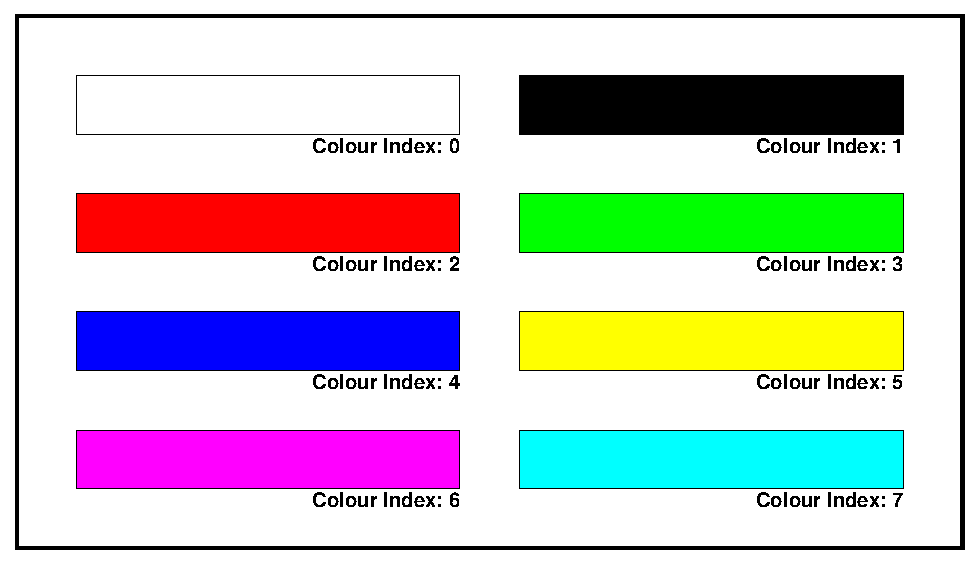
\epsfig{file=col8.eps}}
\caption{\PS~grey level simulation of the eight basic colours.}
\label{COLPS}
\end{figure}
%
\subsubsection{Polyline colour index.}
\index{polyline!colour index}
\index{colour!polyline}
\Shubr[GKS]{ISPLCI}{(ICOLI)}
\Action
This routine sets the polyline colour index attribute for use by future
invocations of \Rind{IPL}. The routine \Rind{IGSET} (see section \ref{IGSET})
can also be used with the parameter \Sind{PLCI}.
\Pdesc
\begin{DLtt}{1234567}
\item[ICOLI] Polyline colour index.
\end{DLtt}
%
\subsubsection{Polymarker colour index.}
\index{polymarker!colour index}
\index{colour!polymarker}
\Shubr[GKS]{ISPMCI}{(ICOLI)}
\Action
This routine sets the polymarker colour index attribute for use by future
invocations of \Rind{IPM}. The routine \Rind{IGSET} (see section \ref{IGSET})
can also be used with the parameter \Sind{PMCI}.
\Pdesc
\begin{DLtt}{1234567}
\item[ICOLI] Polymarker colour index.
\end{DLtt}
%
\subsubsection{Fill area colour index.}
\index{fill area!colour index}
\index{colour!fill area}
\Shubr[GKS]{ISFACI}{(ICOLI)}
\Action
This routine sets the fill area colour index attribute for use by future
invocations of \Rind{IFA}. The routine \Rind{IGSET} (see section \ref{IGSET})
can also be used with the parameter \Sind{FACI}.
\Pdesc
\begin{DLtt}{1234567}
\item[ICOLI] Fill area colour index.
\end{DLtt}
%
\clearpage
\subsubsection{Text colour index.}
\index{text!colour index}
\index{colour!text}
\Shubr[GKS]{ISTXCI}{(ICOLI)}
\Action
This routine sets the text colour index attribute for use by future invocations
of \Rind{ITX}. The routine \Rind{IGSET} (see section \ref{IGSET}) can also be
used with the parameter \Sind{TXCI}.
\Pdesc
\begin{DLtt}{1234567}
\item[ICOLI]Text colour index.
\end{DLtt}
%
\subsection{Fill area interior style}
\index{fill area!interior style}
\Shubr[GKS]{ISFAIS}{(INTS)}
\Action
This routine sets the fill area interior style attribute for use by future
invocations of \Rind{IFA}. The routine \Rind{IGSET} (see section \ref{IGSET})
can also be used with the parameter \Sind{FAIS}.
\Pdesc
\begin{DLtt}{1234567}
\item[INTS] Fill area interior style. Possible values are:
\begin{DLtt}{123}
\item[0] Hollow: the perimeter of the filled area, after clipping, is drawn
         using solid lines.
\item[1] Solid: the area is filled solidly.
\item[2] Pattern: the area is filled with a dot-dashed pattern.
\item[3] Hatched: the area is filled according to the current
value of the fill area style index.
\end{DLtt}
\end{DLtt}
\begin{Fighere}
\begin{center}\mbox{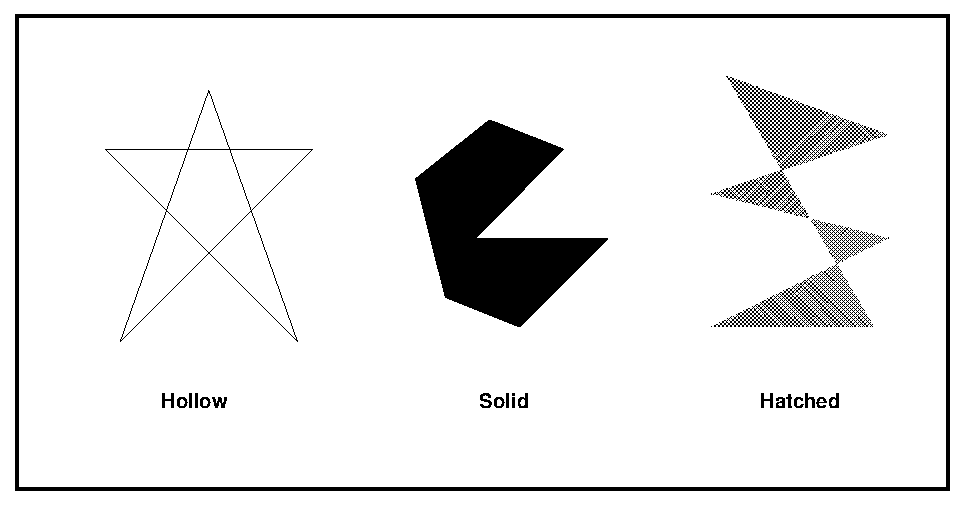
\epsfig{file=fais.eps,width=\the\textwidth}}\end{center}
\caption{Example of fill area interior style.}
\label{FILL-IS}
\end{Fighere}
%
\newpage
\subsection{Fill area style index.}
\index{fill area!style index}
\Shubr[GKS]{ISFASI}{(ISTYLI)}
\Action
This routine sets the fill area style index for pattern and hatch styles. The
routine \Rind{IGSET} (see section \ref{IGSET}) can also be used with the
parameter \Sind{FASI}.
\Pdesc
\begin{DLtt}{1234567}
\item[ISTYLI] Fill area style index. This value depends on the \UGP~used.
\end{DLtt}
In addition to the \UGP~dependent Fill area style indices, \HIGZ~provides a set
of hatches independent from the \UGP~used. This fill area styles are indicated
by a value greater than 100. The fill area style index is coded on three digits
{\tt ijk}.
\begin{DLtt}{1234567}
\item[i] Distance between lines in the hatch.
\item[j] Angle between 90 and 180 degrees.
\item[k] Angle between  0 and  90 degrees.
\end{DLtt}
\begin{center}
\begin{tabular}{||c|c||c|c||c|c||}
\hline
Digit i  &      Distance      &  Digit j  &  Angle  &   Digit k  &  Angle  \\
\hline
         &                    &     0     & 180 deg &     0      &   0 deg \\
  1      & $\approx$ 0.75 mm  &     1     & 170 deg &     1      &  10 deg \\
  2      & $\approx$ 1.50 mm  &     2     & 160 deg &     2      &  20 deg \\
  3      & $\approx$ 2.25 mm  &     3     & 150 deg &     3      &  30 deg \\
  4      & $\approx$ 3.00 mm  &     4     & 135 deg &     4      &  45 deg \\
  5      & $\approx$ 3.75 mm  &     5     &not drawn&     5      &not drawn\\
  6      & $\approx$ 4.50 mm  &     6     & 120 deg &     6      &  60 deg \\
  7      & $\approx$ 5.25 mm  &     7     & 110 deg &     7      &  70 deg \\
  8      & $\approx$ 6.00 mm  &     8     & 100 deg &     8      &  80 deg \\
  9      & $\approx$ 6.75 mm  &     9     &  90 deg &     9      &  90 deg \\
\hline
\end{tabular}
\end{center}
For example {\tt 190} will set the interior of fill areas to be hatched with
lines at 0 and 90 degrees ($\approx$ 0.75 mm spacing) and {\tt 444} will set
the interior of fill areas to be hatched with lines at +45 and -45 degrees
($\approx$ 3 mm spacing).

The figure \ref{FILL-STY} shows some examples of \HIGZ~portable hatch styles.
On this figure, the first column shows the nine different possible spacing
(digit {\tt i}), the second column shows the angle between {\tt 90} and
{\tt 180} degrees (digit {\tt j}), and the third column shows the angle between
{\tt 0} and {\tt 90} degrees (digit {\tt k}).

The number of possible hatch styles is: $9\times10\times10=900$.
\begin{figure}[p]
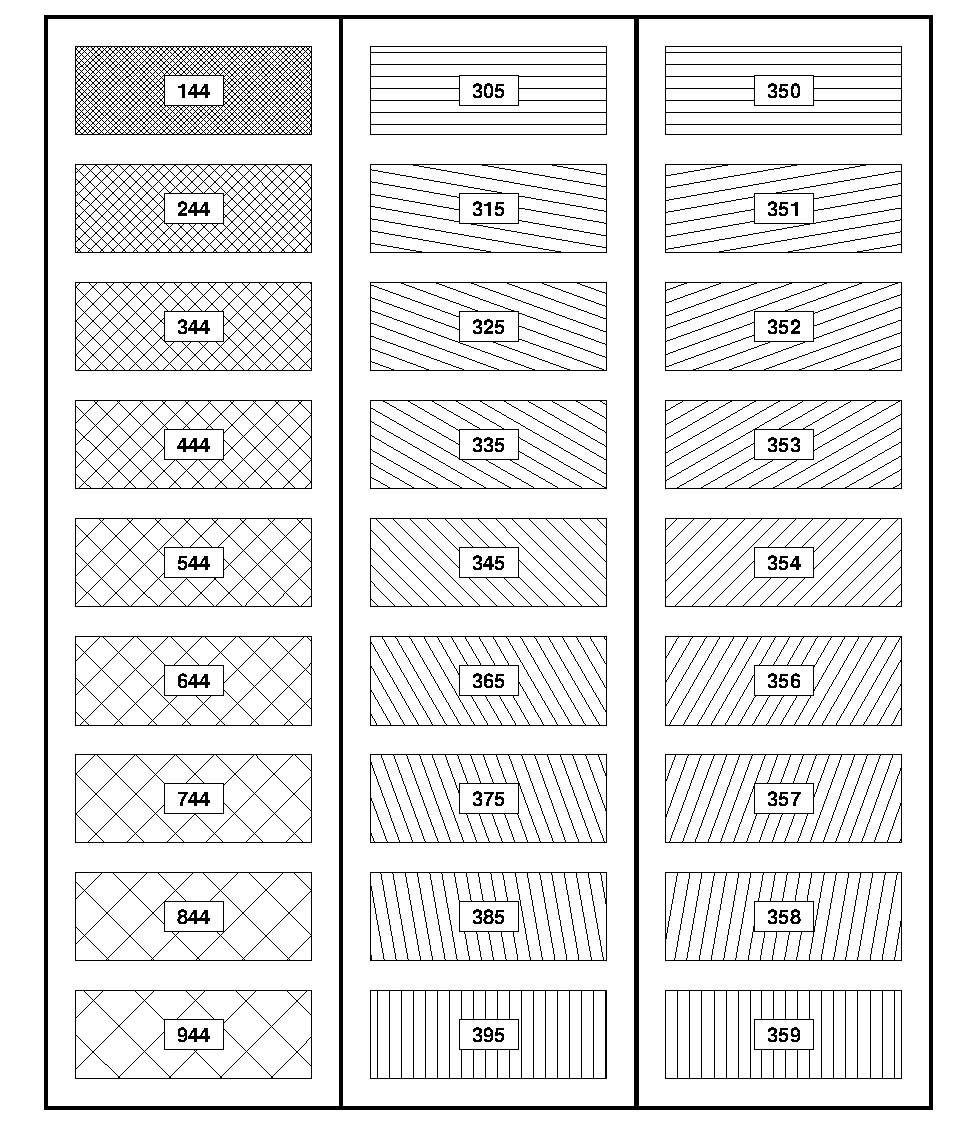
\epsfig{file=fasi.eps,width=\textwidth}
\caption{\HIGZ~portable fill area hatch styles.}
\label{FILL-STY}
\end{figure}
\clearpage
%
\subsection{Line type.}
\index{polyline!type}
\Shubr[GKS]{ISLN}{(LTYPE)}
\Action
This routine sets the line type attribute for use by future invocations of
\Rind{IPL}. All workstations support at least line types 1 through 4
(see figure \ref{LINE-TYPE}). Other line types may be supported. If a requested
line type is not supported on a workstation, line type 1 is used when polylines
are created.
The routine \Rind{IGSET} (see section \ref{IGSET}) can also be used with the
parameter \Sind{LTYP}.
\Pdesc
\begin{DLtt}{1234567}
\item[LTYPE] Line type (positive number).
\begin{DLtt}{123}
\item[1] Solid lines
\item[2] Dashed lines
\item[3] Dotted lines
\item[4] Dashed-dotted lines
\end{DLtt}
\end{DLtt}
\par
Note that line type values are dependent upon the \UGP~used. For the user's
convenience, \HIGZ~defines a number of line types, indicated in the figure
\ref{LINE-TYPE}, which are independent from the basic graphics package used.
%
\subsection{Line width scale factor.}
\index{polyline!width}
\Shubr[GKS]{ISLWSC}{(WIDTH)}
\Action
This routine sets the width of a line for use by future invocations of the
polyline drawing routine \Rind{IPL}. The actual line width is determined by a
nominal line width (workstation-dependent) multiplied by the line width scale
factor. The nominal line width is one pixel on screens. On \PS~printers the
nominal line width is one ``dot''. Therefore the width of a line can vary from
a printer to another depending on the printer definition (300 dots per inch,
400 dots per inch etc.). The figure \ref{LINE-WIDTH} shows some examples of
various line width. The routine \Rind{IGSET} (see section \ref{IGSET}) can also
be used with the parameter \Sind{LWID}.
\Pdesc
\begin{DLtt}{1234567}
\item[WIDTH] Line width scale factor.
\end{DLtt}

\begin{figure}[p]
\begin{center}\mbox{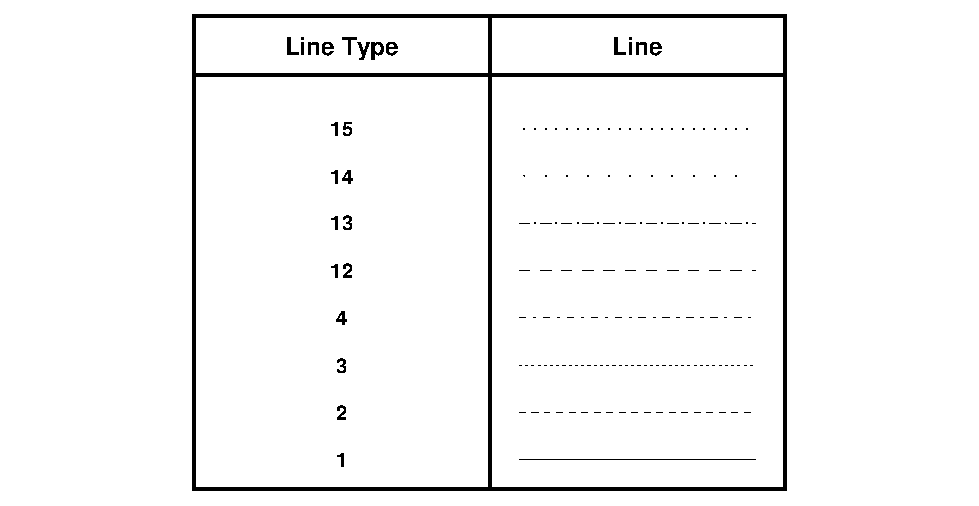
\epsfig{file=line.eps}}\end{center}
\caption{Line styles available.}
\label{LINE-TYPE}

\bigskip

\begin{center}\mbox{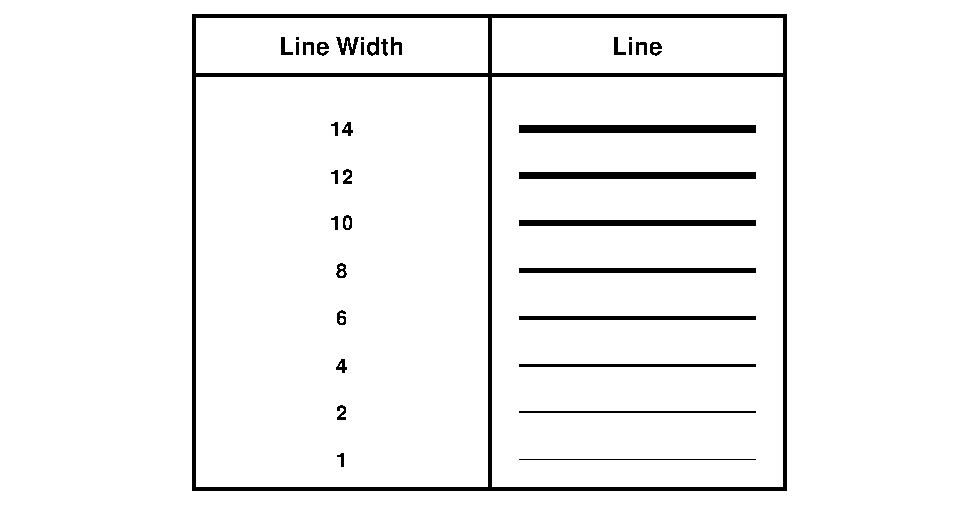
\epsfig{file=linew.eps}}\end{center}
\caption{Examples of line width.}
\label{LINE-WIDTH}
\end{figure}
\clearpage
%
\subsection{Marker type}
\index{polymarker!type}
\Shubr[GKS]{ISMK}{(MTYPE)}
\Action
This routine sets the marker type attribute for use by future invocations of
\Rind{IPM}. All workstations support at least the marker types 1 through 5
(see below). More marker types may be supported by the \UGP. Marker types 20 to
31 are also defined, according to the figure~\ref{MARKER-TYPE}, and are
independent from the \UGP~used. If a requested marker type is not supported on a
workstation, marker type 1 (a point) is used when polymarkers are created.
The routine \Rind{IGSET} (see section \ref{IGSET}) can also be used with the
parameter \Sind{MTYP}.
\Pdesc
\begin{DLtt}{1234567}
\item[MTYPE] Marker type (positive number)
\begin{DLtt}{123}
\item[1] Point shape ($\cdot$).
\item[2] Plus shape ($+$).
\item[3] Asterisk shape ($\ast$).
\item[4] Circle shape ($\circ$).
\item[5] X shape ($\times$).
\end{DLtt}
\end{DLtt}
%
\subsection{Marker scale factor.}
\index{polymarker!scale factor}
\Shubr[GKS]{ISMKSC}{(SSFM)}
\Action
This routine sets the marker scale factor. This scale factor is applied on
the nominal size of the marker. On all workstation, except \PS{} files, the marker
type 1 is not scalable. The routine \Rind{IGSET} (see section \ref{IGSET}) can
also be used with the parameter \Sind{MSCF}.
\Pdesc
\begin{DLtt}{1234567}
\item[SSFM] Scale factor applied to markers. (\(\geq0.\))
\end{DLtt}

\begin{figure}[p]
\begin{center}\mbox{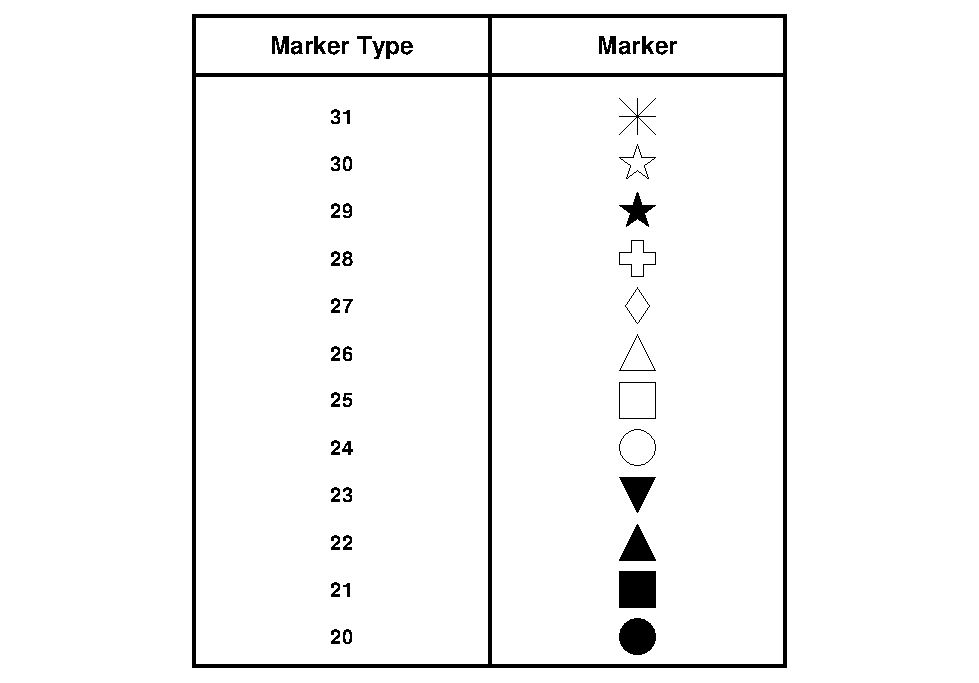
\epsfig{file=marker.eps}}\end{center}
\caption{\HIGZ~Marker type (20-31).}
\label{MARKER-TYPE}

\bigskip

\begin{center}\mbox{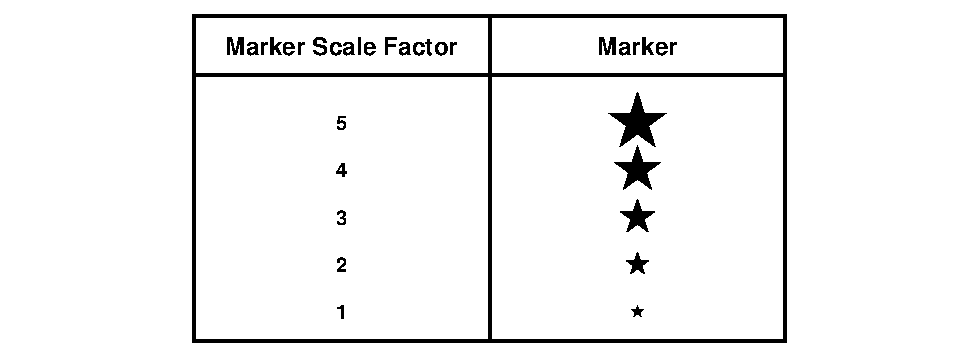
\epsfig{file=markersf.eps}}\end{center}
\caption{Examples marker scale factor.}
\label{MARKER-SIZE}
\end{figure}
\clearpage
%
\subsection{Text alignment.}
\index{text!alignment}
\Shubr[GKS]{ISTXAL}{(ITXALH,ITXALV)}
\Action
This routine sets the text alignment attribute for use by future invocations
of \Rind{ITX}. Text alignment controls the placement of the character string
with respect to the position specified in the call to \Rind{ITX}. Horizontal
alignment specifies which end of the string (or its geometric center) is
aligned with the point specified in \Rind{ITX}. For a given horizontal
alignment, the vertical alignment controls whether the tops of tall characters
or the bottoms of capital letters line up with the point specified (see figure
\ref{TEXT-ALIGN}). The routine \Rind{IGSET} (see section \ref{IGSET}) can also
be used with the parameter \Sind{TXAL}.
\Pdesc
\begin{DLtt}{1234567}
\item[ITXALH] Horizontal alignment specifier ({\tt0$\leq$ITXALH$\leq$3})
\begin{DLtt}{123}
\item[0] Left end of string at point specified (normal).
\item[1] Same as {\tt 0}.
\item[2] Center of string at point specified.
\item[3] Right end of string at point specified.
\end{DLtt}
\item[ITXALV] Vertical alignment specifier ({\tt0\(\leq\)ITXALV\(\leq\)5})
\begin{DLtt}{123}
\item[0] Base of the characters (normal).
\item[1] Top of tallest characters.
\item[2] Same as {\tt 2}.
\item[3] Middle of tallest characters.
\end{DLtt}
\end{DLtt}
\begin{Fighere}
\begin{center}\mbox{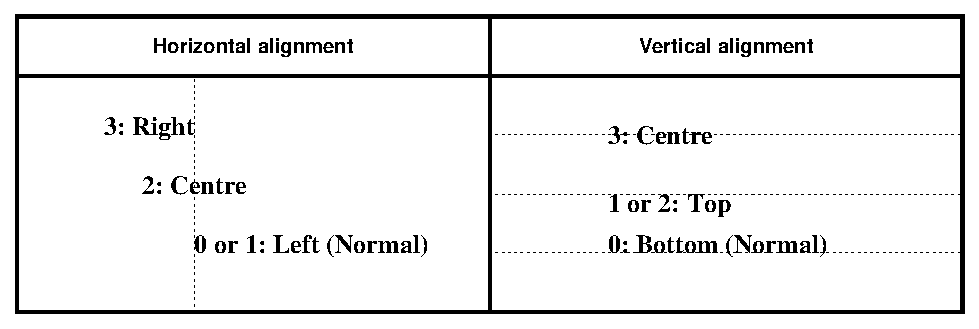
\epsfig{file=align.eps}}\end{center}
\caption{Text alignment.}
\label{TEXT-ALIGN}
\end{Fighere}
%
\newpage%%%%%%%%%%%%%%%%%%%%%%%%%%%%%%%%%%%%%%%%%%%%%%%%%%%%%%%%%%%%%%%%%%%%%%
\subsection{Character height}
\index{text!character height}
\Shubr[GKS]{ISCHH}{(CHH)}
\Action
This routine sets the character height attribute for use by future invocations
of \Rind{ITX}. The routine \Rind{IGSET} (see section \ref{IGSET}) can also be
used with the parameter \Sind{CHHE}.
\Pdesc
\begin{DLtt}{1234567}
\item[CHH] Character height. The default set by \Rind{IGSSE} is {\tt0.01}. The
           height is given in \WC~and it must be positive.
\end{DLtt}
%
\subsection{Character up vector.}
\index{text!character up vector}
\index{text!angle}
\Shubr[GKS]{ISCHUP}{(RCHUX, RCHUY)}
\Action
This routine sets the ``character up vector'' attribute for use by future
invocations of \Rind{ITX}. The angle of the text can also be specified via the
\Rind{IGSET} routine with the parameter \Sind{TANG}.
\Pdesc
\begin{DLtt}{1234567}
\item[RCHUX] Character up vector in \WC~(x part).
\item[RCHUY] Character up vector in \WC~(y part).
\end{DLtt}
The size of the vector specified is immaterial, but
{\tt CHUX$^2$+CHUY$^2$>1.E-20}.
%
\subsection{Text font and precision.}
\index{text!font and precision}
\Shubr[GKS]{ISTXFP}{(IFONT,IPREC)}
\Action
This routine sets the text font and precision attributes for use by future
invocations of \Rind{ITX}. The text font parameter selects among possible
character shapes, as a roman font, a sans-serif font, etc. The text precision
parameter specifies how closely \HIGZ~(and also the \UGP) must follow the
current size and orientation attributes. String precision is most liberal,
stroke precision is most strict. Character precision is in the middle.
The routine \Rind{IGSET} (see section \ref{IGSET}) can also be used with the
parameter \Sind{TXFP}.
\Pdesc
\begin{DLtt}{1234567}
\item[IFONT] Text font. The value of {\tt IFONT} depends on the \UGP~used.
\item[IPREC] Text precision ({\tt0\(\leq\)IPREC\(\leq\)2}).
\end{DLtt}
Note that font number 0, with precision 2, is always available, independently
from the \UGP~used and allows to access the \Rind{IGTEXT} facilities from
\Rind{ITX}. If a font is not available on a workstation, or it is supported
but not with the requested precision, font 1 is used, with precision 0.
\subsubsection{The \PS~text fonts}
\index{PostScript!fonts}
\index{PostScript!fonts!Times-Italic}
\index{PostScript!fonts!Times-Bold}
\index{PostScript!fonts!Times-BoldItalic}
\index{PostScript!fonts!Helvetica}
\index{PostScript!fonts!Helvetica-Oblique}
\index{PostScript!fonts!Helvetica-Bold}
\index{PostScript!fonts!Helvetica-BoldOblique}
\index{PostScript!fonts!Courier}
\index{PostScript!fonts!Courier-Oblique}
\index{PostScript!fonts!Courier-Bold}
\index{PostScript!fonts!Courier-BoldOblique}
\index{PostScript!fonts!Symbol}
\index{PostScript!fonts!Times-Roman}
\index{PostScript!fonts!ZapfDingbats}
With \PS~work\-sta\-tion types, the text pro\-du\-ced by \Rind{ITX} can be
ge\-ne\-ra\-ted with \PS~fonts. The figure \ref{PS-FONT} shows all the \PS~fonts
avai\-lable on most \PS~prin\-ters. Note that the fonts {\tt -15} to {\tt -24}
are the same than {\tt -1} to {\tt -14}, but they are drawn in hollow mode.

The {\sf ZapfDingbats} font is not available on all \PS~printers. On such
printers \index{PostScript!printers} a reference to this font will produce an
error message. The correspondence between \ASCII~and {\sf ZapfDingbats} font
is given on figures \ref{PSTEXT1} and \ref{PSTEXT2}.
\Rind{IGTEXT} control characters are taken into account. In addition
the character $\sim$ switches to the ZapfDingbats character set.
\index{lower case letters}
\index{upper case letters}
\index{Greek letters}
\index{superscript}
\index{subscript}
\index{backspace}
\index{termination character}
\index{special symbols}
\begin{center}
\begin{tabular}{||c|l||c|l||}
\hline
\multicolumn{4}{|c|}{\bf List of escape characters and their meaning}      \\
\hline
 $<$  & go to lower case (optional)      & $>$  & go to upper case (optional)\\
\hline
 \lsb & go to greek (Roman = default)    & \rsb & end of greek               \\
\hline
 "    & go to special symbols            & \#   & end of special symbols     \\
\hline
$\sim$ & go to ZapfDingbats               & \#   & end of ZapfDingbats        \\
\hline
$\uparrow$  & go to superscript          & ?    & go to subscript            \\
\hline
 !    & go to normal level of script     & \&   & backspace one character    \\
\hline
 \$   & termination character (optional) &      &                            \\
\hline
\end{tabular}
\end{center}
\par
The \PS~fonts can with precision {\tt 0} or precision {\tt 1}.
On the screen, a \PS~font used with precision {\tt 1} appears
like the \Rind{IGTEXT} characters, with precision 0 its appears as
hardware character. In both cases the \PS~file is the same.

Note that characters can also be entered directly in lower or upper case
instead of using the escape characters {\tt <} and {\tt >}.

\begin{XMPt}{Example of \PS~ text (result in figure \ref{PSEX1})}
      program psex1
      call start('psex1',16.,5.)
      call igset('LWID',6.)
      call igbox(0.,16.,0.,5.)
      call igset('CHHE',0.5)
      call igset('TXAL',3.)
      call igset('TXFP',-130.)
*
      call itx(3.,4.,'K\bs{}355nstler in den gr\bs{}345\bs{}373ten st\bs{}311dten')
      call itx(3.,3.,'\bs{}253\bs{}265 l''\bs{}372uvre on conna\bs{}333t l''artisan\bs{}273')
      call itx(3.,2.,'\bs{}(proverbe fran\bs{}321ais\bs{}).')
      call itx(3.,1.,'\bs{}252\bs{}241ma\bs{}337ana!\bs{}272, dit l''\bs{}323l\bs{}325ve.')
*
      call finish
      end
\end{XMPt}

\begin{Fighere}
\begin{center}\mbox{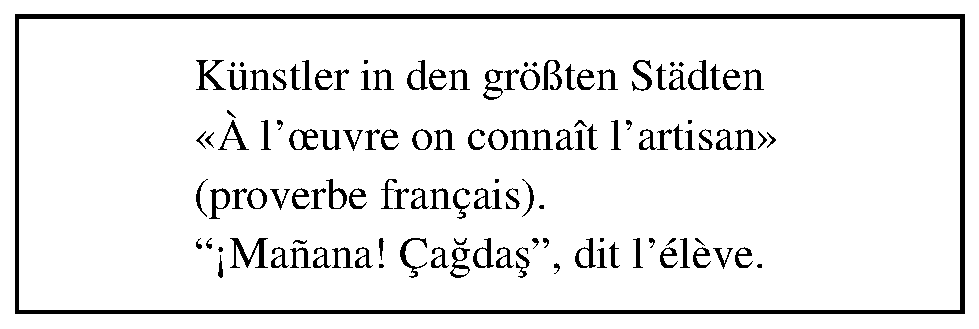
\epsfig{file=psex1.eps}}\end{center}
\caption{\PS~fonts usage (1).}
\label{PSEX1}
\end{Fighere}

\newpage%%%%%%%%%%%%%%%%%%%%%%%%%%%%%%%%%%%%%%%%%%%%%%%%%%%%%%%%%%%%%%%%%%%

\begin{XMPt}{Example of \PS~ text and maths (result in figure \ref{PSEX2})}
      program psex2
      call start('psex2',16.,5.)
      call igset('LWID',6.)
      call igbox(0.,16.,0.,5.)
      call igset('CHHE',0.5)
      call igset('TXAL',23.)
      call igset('TXFP',-130.)
*
      call itx(8.,4.,
     +'e^+!e^-! "5# Z^o! "5# ll&^-!, qq&^\bs{}261!')
      call itx(8.,3.,
     +'| a&^[\bs{}256]! \bs{}267 b&^[\bs{}256]! | = [\bs{}345] a^i?jk!+b^kj?i')
      call itx(8.,2.,
     + 'i ("d#?[m!y]&^\bs{}261![g^m]! + m [y]&^\bs{}261! ) = 0'//
     + '" r# (~r# + m^2!) [y] = 0')
      call itx(8.,1.,
     + 'L?em! = e J^[m]?em! A?[m]! , J^[m]?em!=l&^\bs{}261![ g?m]!l , '//
     + 'M^j?i! = [\bs{}345&?a]! A?[a! t^a]j?i! ')
*
      call finish
      end
\end{XMPt}

\begin{Fighere}
\begin{center}\mbox{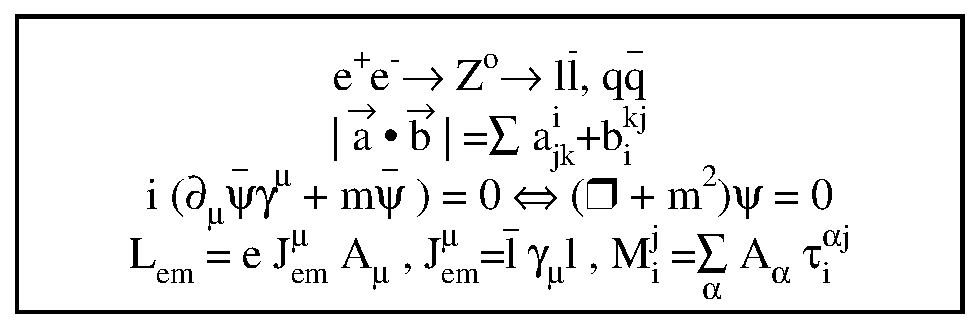
\epsfig{file=psex2.eps}}\end{center}
\caption{\PS~fonts usage (2).}
\label{PSEX2}
\end{Fighere}

\begin{figure}[p]
\begin{center}\mbox{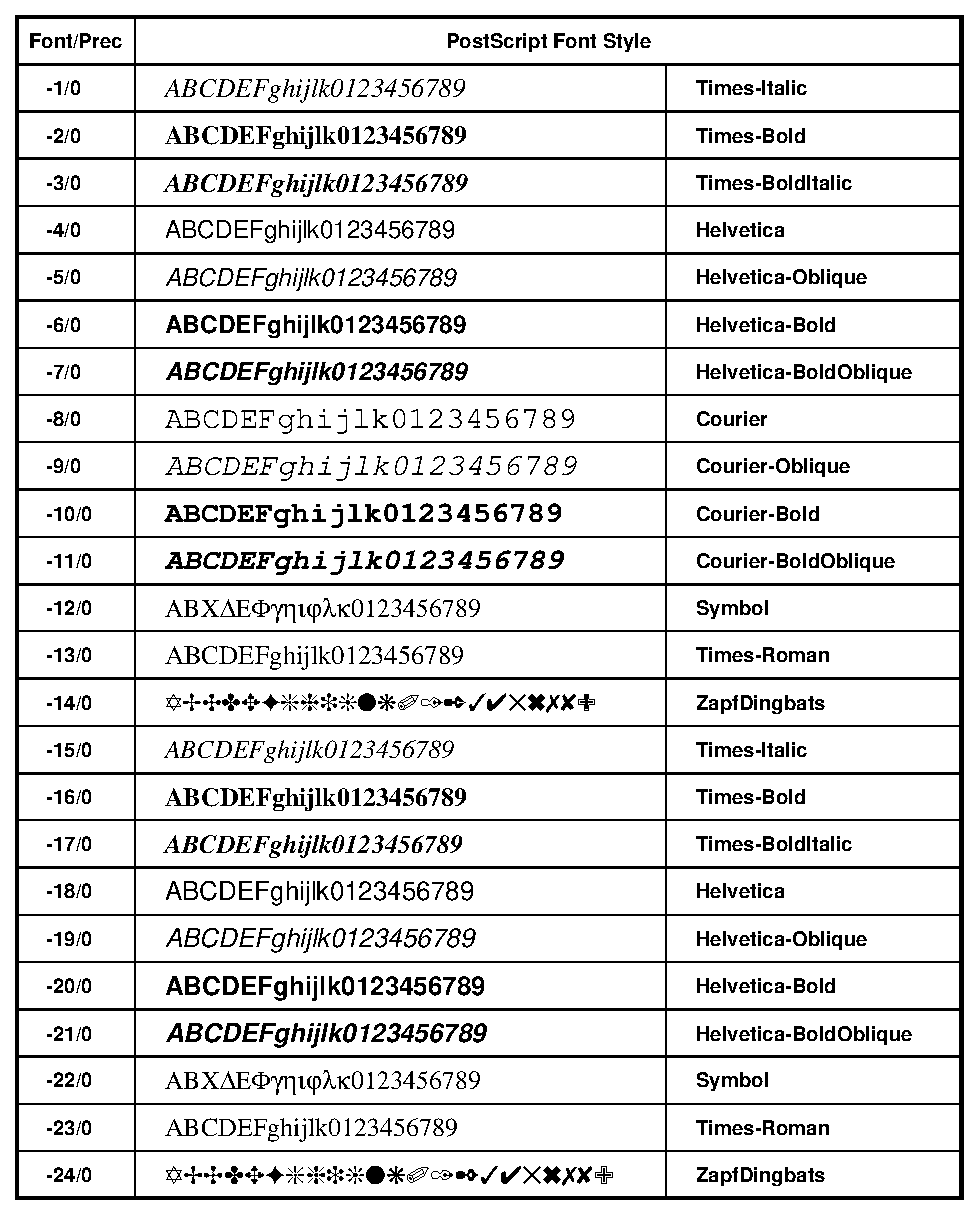
\epsfig{file=psfont.eps,width=\the\textwidth}}\end{center}
\caption{\PS~ text fonts.}
\label{PS-FONT}
\end{figure}

\begin{figure}[p]
\begin{center}\mbox{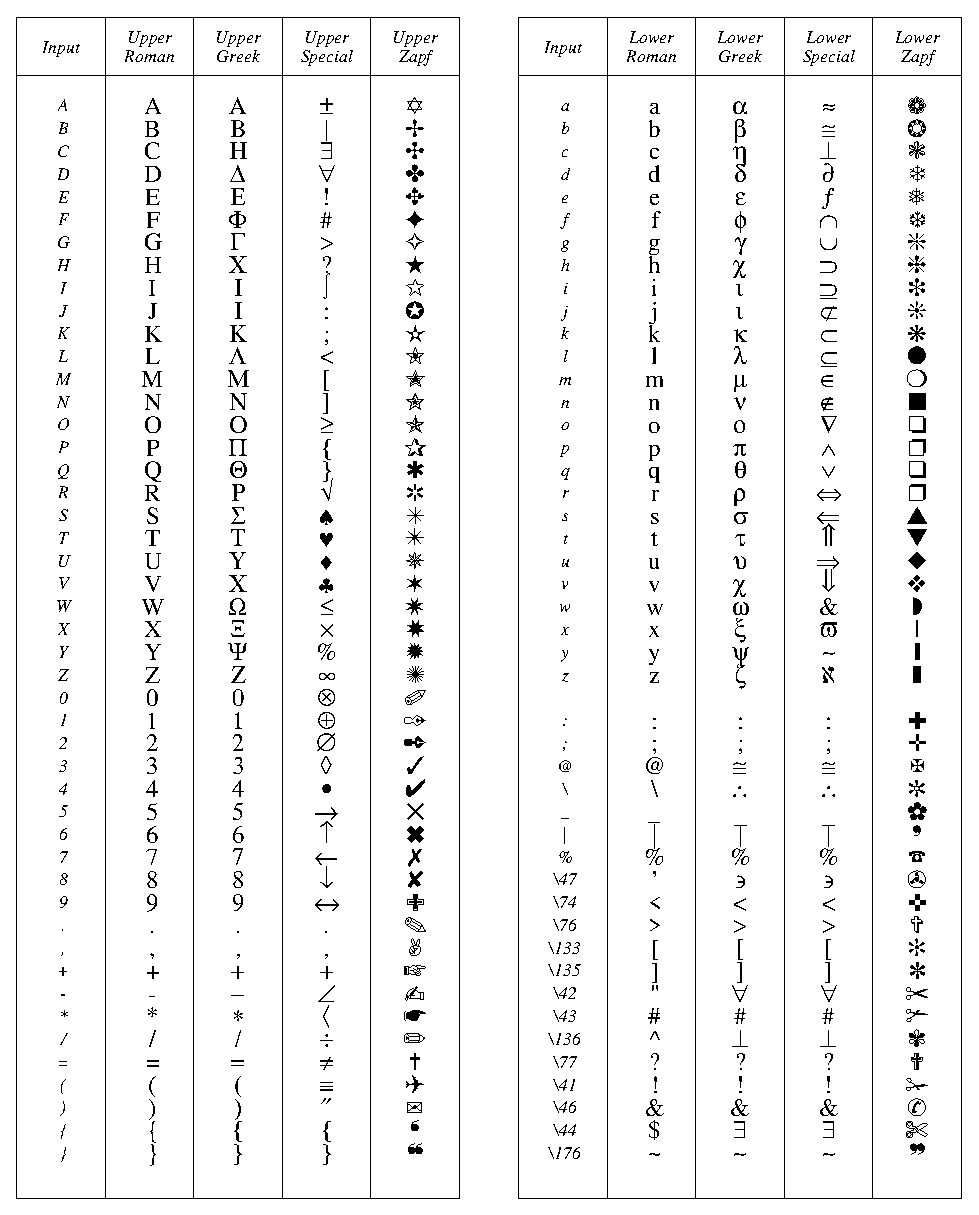
\epsfig{file=pstext1.eps,width=\the\textwidth}}\end{center}
\caption{\PS~ characters (1).}
\label{PSTEXT1}
\end{figure}

\begin{figure}[p]
\begin{center}\mbox{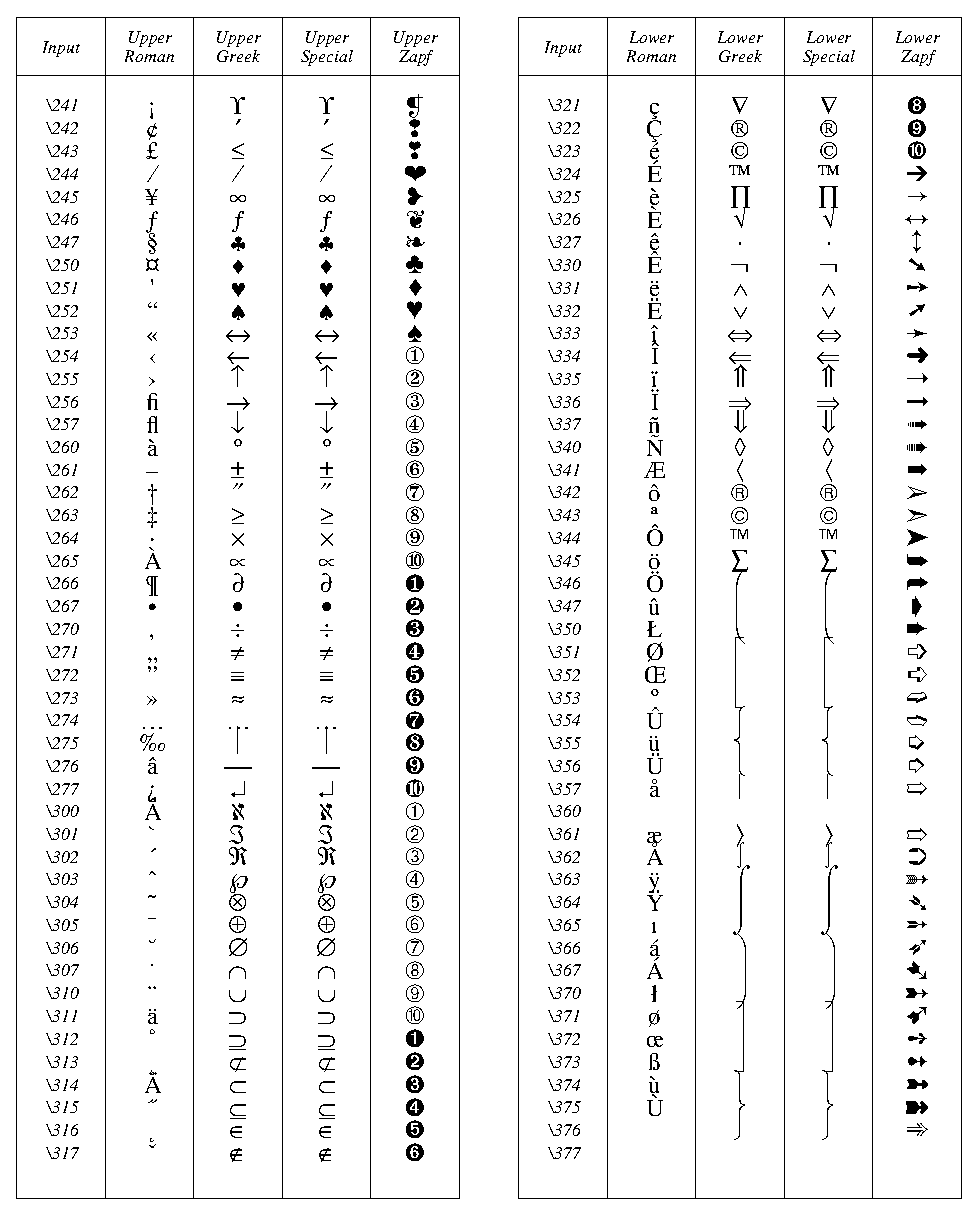
\epsfig{file=pstext2.eps,height=19cm}}\end{center}
\caption{\PS~ characters (2).}
\label{PSTEXT2}
\end{figure}
\clearpage
         % Basic graphics routines
%%%%%%%%%%%%%%%%%%%%%%%%%%%%%%%%%%%%%%%%%%%%%%%%%%%%%%%%%%%%%%%%%%%%%%%%%%%%%%%%
%                                                                              %
%   HIGZ  User Guide -- LaTeX Source                                           %
%                                                                              %
%   Chapter: Graphics macroprimitives                                          %
%                                                                              %
%   This document needs the following external EPS files:                      %
%            box.eps                                                           %
%            fbox.eps                                                          %
%            pave.eps                                                          %
%            arc.eps                                                           %
%            graph.eps                                                         %
%            hist.eps                                                          %
%            scatter.eps                                                       %
%            boxes.eps                                                         %
%            arrows.eps                                                        %
%            contour.eps                                                       %
%            colour.eps                                                        %
%            tabt.eps                                                          %
%            tabk.eps                                                          %
%            lego.eps                                                          %
%            lego1.eps                                                         %
%            lego2.eps                                                         %
%            surf.eps                                                          %
%            surf1.eps                                                         %
%            surf2.eps                                                         %
%            surf3.eps                                                         %
%            surf4.eps                                                         %
%            surfpol.eps                                                       %
%            surfcyl.eps                                                       %
%            surfsph.eps                                                       %
%            surfpsd.eps                                                       %
%            pie.eps                                                           %
%            higzaxis.eps                                                      %
%            softtext.eps                                                      %
%                                                                              %
%   Editor: Olivier Couet / CN-AS                                              %
%   Last Mod.: 9 July 1993 oc                                                  %
%                                                                              %
%%%%%%%%%%%%%%%%%%%%%%%%%%%%%%%%%%%%%%%%%%%%%%%%%%%%%%%%%%%%%%%%%%%%%%%%%%%%%%%%
\Filename{H1Thegraphicmacroprimitives}
\chapter{The graphic macroprimitives}
\index{graphic!macroprimitives}

In addition to the standard set of basic graphic primitives describe
in the previous chapter, \HIGZ~provides also a set of graphic "macroprimitives".
\index{macroprimitive} 
These graphic macroprimitives are included in \HIGZ~for three main reasons:
\begin{enumerate}
\item Functionality: it is easier to define a circle with its center and its
      radius than to compute all the necessary points to draw a polyline.
\item Precision, for instance a circle has to be stored as a circle and not as
      a sequence of polylines.
\item Compactness of the graphic data base.
\index{picture!data base}
\end{enumerate}
 
\Filename{H2Drawingabox}
\section{Drawing a box}
\index{box!drawing}
\Shubr{IGBOX}{(X1,X2,Y1,Y2)}
\Action
This routine fills a rectangle according to the ``fill area colour index''
(see section \ref{ISFACI}), the ``fill area interior style'' (see section
\ref{ISFAIS}), and the ``fill area style index'' (see section \ref{ISFASI})
attributes. The border is never drawn unless the interior
style is hollow or the routine \Rind{IGSET} has been called with '\Sind{BORD}'
and {\tt VAL = 1.}. As it is shown on the figure \ref{BOX}, the border of the
rectangle is drawn according to the values of the ``line width scale factor''
(see section \ref{ISLWSC}) and the ``polyline colour index'' (see section
\ref{ISPLCI}) attributes, whereas the ``line type'' is always solid (see
section \ref{ISLN}).
\Pdesc
\begin{DLtt}{123}
\item[X1] X coordinate of 1st corner of the rectangle in \wc.
\item[X2] X coordinate of 2nd corner of the rectangle in \wc.
\item[Y1] Y coordinate of 1st corner of the rectangle in \wc.
\item[Y2] Y coordinate of 2nd corner of the rectangle in \wc.
\end{DLtt}

\begin{Fighere}
\begin{center}\mbox{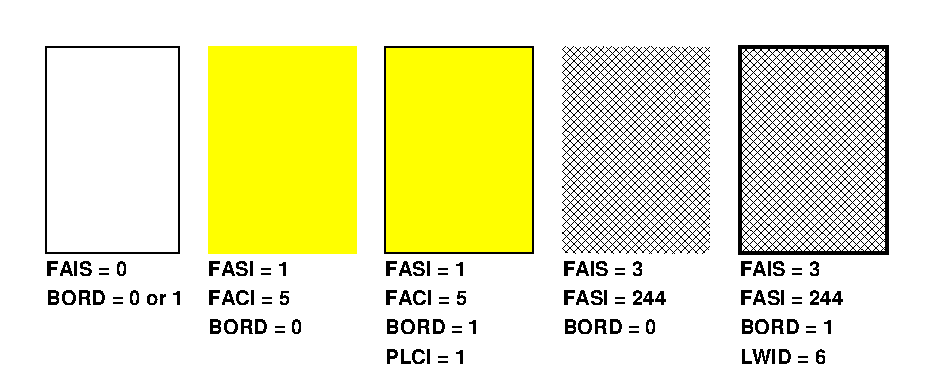
\epsfig{file=box.eps}}\end{center}
\caption{Action of the fill area and polyline attributes on 
\protect\Rind{IGBOX}.}
\label{BOX}
\end{Fighere}
 
\vfill\newpage
\Filename{H2Drawingaframe}
\section{Drawing a frame}
\index{frame!drawing}
\Shubr{IGFBOX}{(X1,X2,Y1,Y2,X3,X4,Y3,Y4)}
\Action
This routine fills a frame according to the ``fill area colour index''
(see section \ref{ISFACI}), the ``fill area interior style'' (see section
\ref{ISFAIS}), and the ``fill area style index'' (see section \ref{ISFASI})
attributes. The border is never drawn unless the interior
style is hollow or the routine \Rind{IGSET} has been called with '\Sind{BORD}'
and {\tt VAL = 1.}. Like for the \Rind{IGBOX} primitive (see figure \ref{BOX}),
the border of the frame is drawn according to the values of the ``line width
scale factor'' (see section \ref{ISLWSC}) and the ``polyline colour index''
(see section \ref{ISPLCI}) attributes, whereas the ``line type'' is always solid
(see section \ref{ISLN}).
\Pdesc
\begin{DLtt}{123}
\item[X1] X coordinate of 1st corner of the outer rectangle in \wc.
\item[X2] X coordinate of 2nd corner of the outer rectangle in \wc.
\item[Y1] Y coordinate of 1st corner of the outer rectangle in \wc.
\item[Y2] Y coordinate of 2nd corner of the outer rectangle in \wc.
\item[X3] X coordinate of 1st corner of the inner rectangle in \wc.
\item[X4] X coordinate of 2nd corner of the inner rectangle in \wc.
\item[Y3] Y coordinate of 1st corner of the inner rectangle in \wc.
\item[Y4] Y coordinate of 2nd corner of the inner rectangle in \wc.
\end{DLtt}
The figure \ref{FBOX} describes the usage of the \Rind{IGFBOX} parameters.

\begin{Fighere}
\begin{center}\mbox{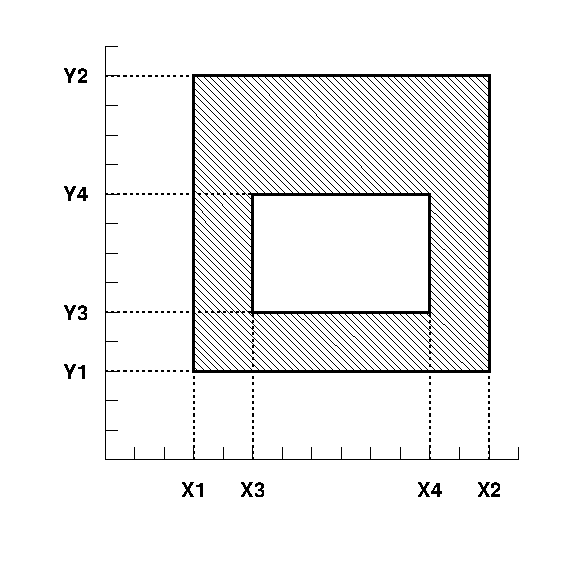
\epsfig{file=fbox.eps}}\end{center}
\caption{Example of \protect\Rind{IGFBOX} usage}
\label{FBOX}
\end{Fighere}
 
\vfill\newpage
\Filename{H2Drawingapavingblock}
\section{Drawing a paving block}
\index{paving block!drawing}
\Shubr{IGPAVE}{(X1,X2,Y1,Y2,DZ,ISBOX,ISFRAM,CHOPT)}
\Action
 This routine draws a paving-block according to the value of {\tt CHOPT}.
 {\tt ISBOX (ISFRAM)} may be {\tt 1000+ICOLOR} where {\tt ICOLOR} is the
colour index of the box (frame), or {\tt 2000+IPAT} where {\tt IPAT} is
the pattern index of the box (frame), otherwise the style index.
If {\tt ISBOX(ISFRAM)=0}, only the box contour is drawn with the current
polyline attributes. By default the Top and the Right frames are drawn.
{\tt CHOPT='TR'}.
\Pdesc
\begin{DLtt}{1234567}
\item[X1]     X bottom left corner of box.
\item[X2]     X top right corner of box.
\item[Y1]     Y bottom left corner of box.
\item[Y2]     Y top right corner of box.
\item[DZ]     Box width.
\item[ISBOX]  Box style.
\item[ISFRAM] Frame style.
\item[CHOPT]  Character option.
\begin{DLtt}{12345}
   \item['T'] The top of the frame is drawn.
   \item['B'] The bottom of the frame is drawn.
   \item['R'] The right part of the frame is drawn.
   \item['L'] The left part of the frame is drawn.
   \item['-'] Reverse sense for the shadow drawing (see figure~\ref{PAVE}).
   \item['S'] The frame is drawn like the ``Shadow'' of the inside box.
   \item['P'] Cut the top of the shadow (see figure~\ref{PAVE}).
   \item['K'] The paving-block is drawn like a button (see figure~\ref{PAVE}).
   \item['D'] Delete. The paving block is drawn in the background colour.
\end{DLtt}
\end{DLtt}
\newpage

\begin{Fighere}
\begin{center}\mbox{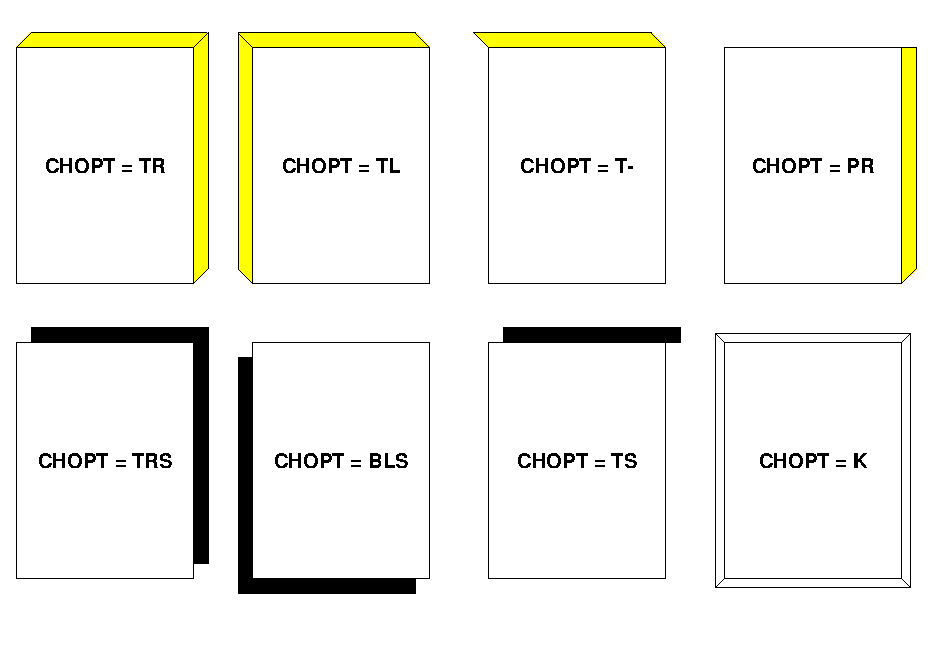
\epsfig{file=pave.eps}}\end{center}
\caption{Examples of \protect\Rind{IGPAVE} usage}
\label{PAVE}
\end{Fighere}
 
\newpage
\Filename{H2Drawinganarc}
\section{Drawing an arc}
\index{arc drawing}
\Shubr{IGARC}{(XC,YC,R1,R2,PHIMIN,PHIMAX)}
\Action
This routine draws one or two arcs of a circle. If the two radii are not equal the area
between the two arcs is filled according to the fill area interior style index
and the fill area style index. The border is never drawn unless the interior
style is hollow or the routine \Rind{IGSET} has been called with \Sind{BORD} and
{\tt VAL = 1}. If the arc's radii are equal only one arc is drawn.
\Pdesc
\begin{DLtt}{1234567}
\item[XC]     X coordinate of the arc's center in world coordinate space.
\item[YC]     Y coordinate of the arc's center in world coordinate space.
\item[R1]     Radius of first arc.
\item[R2]     Radius of second arc.
\item[PHIMIN] Starting angle (degrees.)
\item[PHIMAX] Final angle (degrees.)
\end{DLtt}

\begin{Fighere}
\begin{center}\mbox{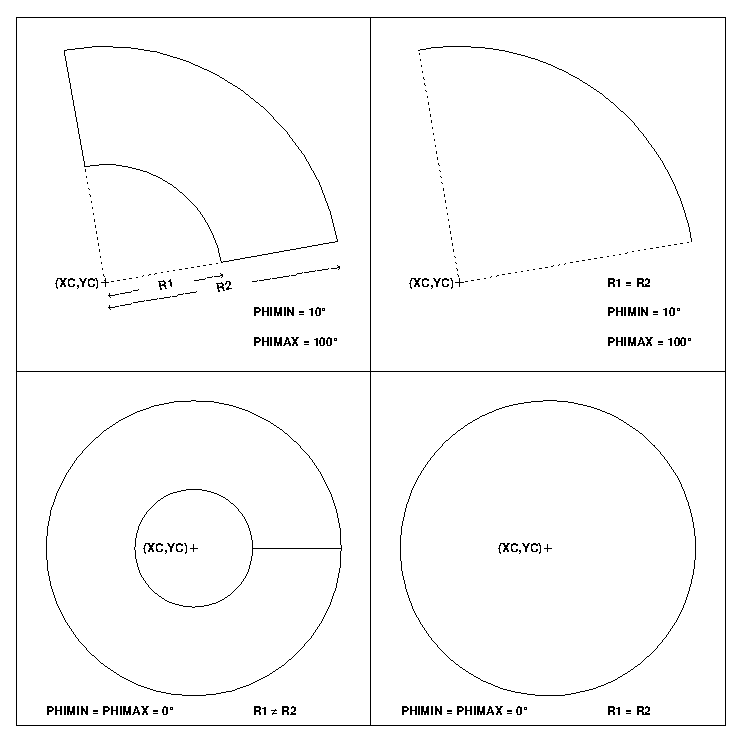
\epsfig{file=arc.eps,height=12cm}}\end{center}
\caption{Examples of \protect\Rind{IGARC}}
\label{fig-FIGU005S}
\end{Fighere}
\vfill
\newpage
\Filename{H2Drawingagraph}
\section{Drawing a graph}
\index{graph drawing}
\Shubr{IGRAPH}{(N,X,Y,CHOPT)}
\Action
This routine draws (in the current \NT) a graph with several possible 
presentations.
\index{curve drawing}
\Pdesc
\begin{DLtt}{1234567}
\item[N]     Number of components in the arrays {\tt X} and {\tt Y}.
\item[X]     Array of dimension {\tt N} containing the x coordinates in
             \WC~space of the graph to be drawn.
\item[Y]     Array of dimension {\tt N} containing the y coordinates in
             \WC~space of the graph to be drawn.
\item[CHOPT] {\tt CHARACTER} variable specifying the options chosen (multiple
             simultaneous options are possible).
\begin{DLtt}{12345}
   \item['R'] The graph is Rotated, i.e. the values in {\tt X} are used
              for the ordinate and the values in {\tt Y} for the abscissa
              (default is the contrary).
   \item['L'] All points are connected with a straight line. (default)
   \item['F'] A Fill area is drawn through the points with the current fill area
              attributes. The border is never drawn unless the fill area 
              interior style is hollow or the routine \Rind{IGSET} has been 
              called with '\Sind{BORD}' and {\tt VAL = 1.}.
   \item['C'] The values in {\tt Y} are plotted in the form of a smooth curve.
              Spline approximation algorithms are used. This option can be used
              with option F in order to draw a smooth fill area.
   \item['*'] A star is plotted at every point.
   \item['P'] A marker is plotted at every point, according to the current
              polymarker attributes.
   \item['B'] The values in {\tt Y} are plotted in the form of bars.
              The width of the bar is by default 50\% of the interval
              {\tt X(I)-X(I-1)}. This percentage can be changed by calling
              \Rind{IGSET} with option \Sind{BARW}.
   \item['A'] X and Y axes are drawn on the border of the current \NT.
   \item['GX'] Logarithmic scale on the X axis.
   \item['GY'] Logarithmic scale on the Y axis.
\end{DLtt}
\end{DLtt}

\newpage
\begin{XMPt}{Example of {\tt GRAPH} drawing (see result on figure \ref{GRAPH})}
      program  graph 
      character*4 chopt(4)
      dimension x(9),y(9)
      parameter (xsize=16.,ysize=20.)
      data x/0.,.6,.3,.2,-.3,.3,-.2,-.3,-.6/
      data y/0.,-.2,-.7,-.9,-.2,.2,.9,.7,.2/
      data chopt/'AL*','AC*','AF*','ACF*'/
*
      call start('graph',xsize,ysize)
*
*              Viewports definition
*
      xnorm  = min(1.,xsize/ysize)
      xnorm2 = xnorm/2.
      ynorm  = min(1.,ysize/xsize)
      ynorm2 = ynorm/2.
      rmarg  = 0.05
      rmarg2 = rmarg/2.
      call isvp(10,rmarg,xnorm2-rmarg2,ynorm2+rmarg2,ynorm-rmarg)
      call isvp(20,xnorm2+rmarg2,xnorm-rmarg,ynorm2+rmarg2,ynorm-rmarg)
      call isvp(30,rmarg,xnorm2-rmarg2,rmarg,ynorm2-rmarg2)
      call isvp(40,xnorm2+rmarg2,xnorm-rmarg,rmarg,ynorm2-rmarg2)
*
*              Some attributes setting
*
      call isclip(0)
      call igset('FASI',244.)
      call igset('BORD',1.)
      call igset('CHHE',.05)
*
*              GRAPH drawing
*
      do i=1,4
         call iswn(10*i,-1.,1.,-1.,1.)
         call iselnt(10*i)
         call igset('FAIS',0.)
         call igbox(-1.,1.,-1.,1.)
         call itx(.3,.9,'CHOPT = '''//CHOPT(I)//'''')
         call igset('FAIS',3.)
         call igraph(9,x,y,chopt(i))
      enddo
      call finish
*
      end
\end{XMPt}

\begin{figure}[p]
\begin{center}
\mbox{}\\[-1cm]
\mbox{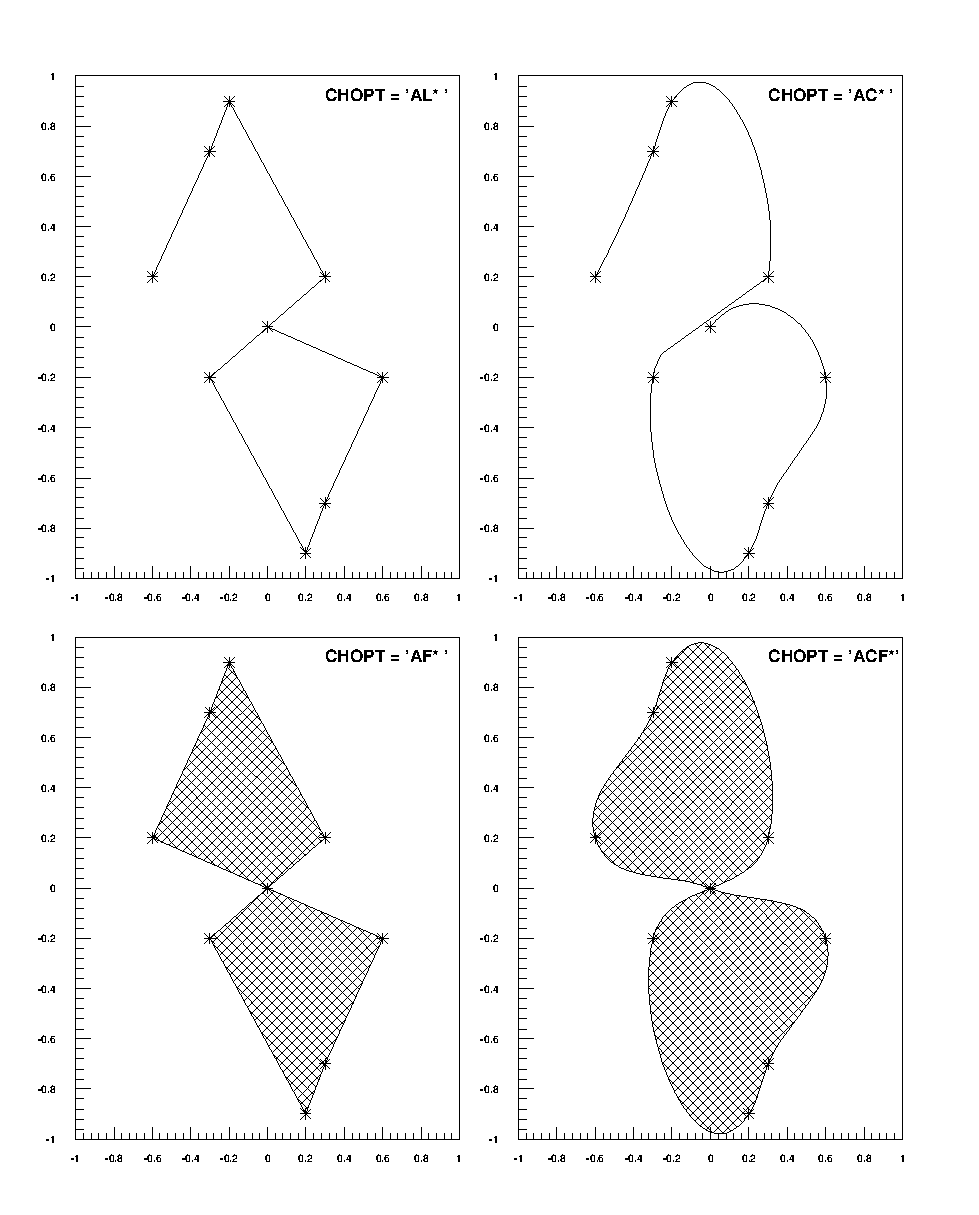
\epsfig{file=graph.eps}}
\end{center}
\caption{Example of \protect\Rind{IGRAPH} using {\tt L,C,F} and {\tt*} options.}
\label{GRAPH}
\end{figure}
\clearpage 

\Filename{H2Drawingahistogram}
\section{Drawing a histogram}
\index{histogram drawing}
\Shubr{IGHIST}{(N,X,Y,CHOPT)}
\Action
This routine draws a one-dimensional histogram with several possible 
presentations chosen by the user (histograms, bars, columns, smoothed graphs,
etc.).
\Pdesc
\begin{DLtt}{1234567}
\item[N] Number of bins in {\tt X} and/or {\tt Y}.
\item[X] Is either an array of dimension {\tt N} containing x
         coordinates or a two-dimensional array with {\tt (XMIN,XMAX)}
         (\WC~space).
\item[Y] Is either an array of dimension {\tt N} containing y
         coordinates or a two-dimensional array with {\tt (YMIN,YMAX)}
         (\WC~space).
\item[CHOPT] {\tt CHARACTER} variable specifying the options
             selected (Multiple simultaneous options are possible).
             Note that the number of components needed in the array {\tt X}
             and/or {\tt Y} may depend on the value of {\tt CHOPT}.
\begin{DLtt}{12345}
   \item['R'] The histogram is Rotated, i.e. the values in {\tt X} are used
              for the ordinate and the values in {\tt Y} for the abscissa
              (default is the contrary). If option {\tt 'R'} is selected (and
              option {\tt 'N'} is not selected), the user must give:
   \begin{UL}
      \item 2 values for {\tt Y} ({\tt Y(1)=YMIN} and {\tt Y(2)=YMAX})
      \item {\tt N} values for {\tt X}, one for each bin.
   \end{UL}
   Otherwise the user must give:
   \begin{UL}
      \item {\tt N} values for {\tt Y}, one for each bin.
      \item 2 values for {\tt X} ({\tt X(1)=XMIN} and {\tt X(2)=XMAX})
   \end{UL}
   For option {\tt 'N'} see below.
   \item['N'] Non equidistant bins (default is equidistant). The arrays {\tt X}
              and {\tt Y} must be dimensioned as follows:
              \\ If option {\tt R} is not selected (default) then the user
               must give:
   \begin{UL}
      \item ({\tt N+1}) values for {\tt X} (the limits of the bins).
      \item {\tt N} values for {\tt Y}, one for each bin.
   \end{UL}
   Otherwise the user must give:
   \begin{UL}
      \item ({\tt N+1}) values for {\tt Y} (the limits of the bins).
      \item {\tt N} values for {\tt X}, one for each bin.
   \end{UL}
   \item['H'] An histogram is drawn as a contour (default).
   \item['F'] The area delimited by the histogram is filled according to the
              fill area interior style and the fill area style index or colour
              index. The contour is not drawn unless the {\tt 'H'} option is
              also selected.
   \item['C'] A smooth curve is drawn across the points at the center of each
              bin of the histogram.
   \item['L'] A straight line is drawn across the points at the center of
              each bin of the histogram.
   \item['*'] A star is plotted at the center of each bin of the histogram.
   \item['P'] The current polymarker is plotted at the center of each bin
              of the histogram.
   \item['B'] A bar chart with equidistant bins is drawn as fill areas
              (contours are drawn). The bar origin and the bar
              width can be controlled by routine \Rind{IGSET} and the
              \Sind{BARO} and \Sind{BARW} options.
   \item['A'] The x and y axes are drawn.
   \item['GX'] Logarithmic scale on the X axis.
   \item['GY'] Logarithmic scale on the Y axis.
\end{DLtt}
\end{DLtt}

\begin{minipage}{\textwidth}
\begin{XMPt}{Example of {\tt HISTOGRAM} drawing (see result on figure 
\ref{HIST})}
      program hist 
      dimension x(2),y(10)
      parameter (xsize=16.,ysize=20.)
      data y/10.,30.,50.,400.,700.,900.,110.,90.,100.,40./
      data x/1.,1000./
*
      call start('hist',xsize,ysize)
*
*              Viewports definition
*
      xnorm  = min(1.,xsize/ysize)
      xnorm2 = xnorm/2.
      ynorm  = min(1.,ysize/xsize)
      ynorm2 = ynorm/2.
      rmarg  = 0.05
      rmarg2 = rmarg/2.
      call isvp(10,rmarg,xnorm2-rmarg2,ynorm2+rmarg2,ynorm-rmarg)
      call isvp(20,xnorm2+rmarg2,xnorm-rmarg,ynorm2+rmarg2,ynorm-rmarg)
      call isvp(30,rmarg,xnorm2-rmarg2,rmarg,ynorm2-rmarg2)
      call isvp(40,xnorm2+rmarg2,xnorm-rmarg,rmarg,ynorm2-rmarg2)
*
*              Some attributes setting
*
      call isclip(0)
      call igset('FASI',244.)
      call igset('FAIS',3.)
      call igset('CHHE',50.)
*
*              HISTOGRAM drawing
*
      call iswn(10,1.,1000.,1.,1000.)
      call iselnt(10)
      call ighist(10,x,y,'AHC*')
*
      call iswn(20,1.,1000.,1.,1000.)
      call iselnt(20)
      call ighist(10,x,y,'AB')
*
      call iswn(30,1.,1000.,log10(1.),log10(1000.))
      call iselnt(30)
      call ighist(10,x,y,'AHFGY')
*
      call iswn(40,log10(1.),log10(1000.),1.,1000.)
      call iselnt(40)
      call ighist(10,x,y,'AHFGX')
*
      call finish
      end
\end{XMPt}
\end{minipage}

\begin{figure}[p]
\begin{center}
\mbox{}\\[-15mm]
\mbox{\epsfig{file=hist.eps}}
\end{center}
\caption{Examples of \protect\Rind{IGHIST} usage.}
\label{HIST}
\end{figure}

\clearpage
 
\Filename{H2Bidimensionalmatrixdrawing}
\section{Bidimensional matrix drawing}
\index{2D matrix!drawing}
\Shubr{IGTABL}{(NX,NY,V,NPAR,PAR,CHOPT)}
\Action
This routine draws a 2D matrix (i.e. table) according to the values of
{\tt CHOPT} and {\tt PAR}. The {\tt PAR} input parameter could be specified 
to change the aspect of the plot (see the description below). The position of
the plot on the screen is given by the viewport of the current \NT~currently
selected (the window is not used and could be anything).
\Pdesc
\begin{DLtt}{12345678}
\item[NX]        Number of cells in X.
\item[NY]        Number of cells in Y.
\item[V(NX,NY)]  Content of the cells.
\item[NPAR]      Number of parameters in \Lit{PAR}.
\item[PAR(NPAR)] Array of real parameter. If \Lit{PAR(i)=0.} or \Lit{NPAR<i} a
                 default value is taken.
\item[CHOPT] {\tt CHARACTER} variable specifying the options selected. The
possible value of {\tt CHOPT} and the associate values of {\tt PAR} are
describe below. The default value of {\tt CHOPT} is \Lit{'P'}.
\end{DLtt}

\begin{XMPt}{Example of {\tt MATRIX} drawing (see result on figure 
\ref{SCATTER} to \ref{SURF4})}
      program matrix 
      call start_matrix('lego','LA')
      call start_matrix('lego1','L1A')
      call start_matrix('lego2','L2')
      call start_matrix('surf','SA')
      call start_matrix('surf1','S1A')
      call start_matrix('surf2','S2A')
      call start_matrix('surf3','S3A')
      call start_matrix('surf4','S4A')
      call start_matrix('surfpol','SPOL')
      call start_matrix('surfcyl','SCYL')
      call start_matrix('surfsph','SSPH')
      call start_matrix('surfpsd','SPSD')
      end

      subroutine start_matrix(name,chopt)
      character*(*) name,chopt
      parameter (nx=30,ny=30)
      dimension v(nx,ny)
      dimension par(29)
*
*              Parameters initialisation
*
      call vzero(par,29)
      par(1)=30.
      par(2)=23.
      par(3)=-10.
      par(4)=10.
      par(5)=-10
      par(6)=10.
      par(9)=1030.
      par(10)=1030.
      par(11)=510.
      par(12)=510.
      par(13)=510.
      par(14)=1.
      par(15)=1.
      par(16)=1.
      par(20)=0.05
      par(21)=-61.
      par(22)=.1
      par(23)=.1
      par(24)=.15
      par(25)=2.
      par(26)=5.
      par(27)=7.
      par(28)=6.
      par(29)=3.
*
*              Matrix filling
*
      x=-10.
      y=-10.
      s=20./float(nx)
      do i=1,nx
         do j=1,ny
            if(x.ne.0..and.y.ne.0)then
               v(i,j)=100.*sin(x)/x*sin(y)/y
            else
               v(i,j)=100.
            endif
            x=x+s
         enddo
         y=y+s
         x=-10.
      enddo
*
*              Matrix drawing
*
      call start(NAME,9.,9.)
      call isfais(0)
      call igset('BORD',1.)
      call igset('TXAL',32.)
      call igset('CHHE',0.25)
      call igtabl(nx,ny,v,29,par,chopt)
      call igterm
      call finish
      end
\end{XMPt}

\begin{figure}[p]
\begin{center}
\begin{tabular}{||c|p{12cm}|>{\tt}r||}
\hline
\multicolumn{3}{||l||}{\bf {\tt CHOPT = 'P'} Polymarker (scatter plot)}          \\
\hline
\multicolumn{1}{||c|}{\bf {\tt PAR} index}        &
\multicolumn{1}{c|}{\bf {\tt PAR} values}         &
\multicolumn{1}{c||}{\bf default}                \\
\hline
 1  & Marker type see \Rind{ISMK}.                                  &   1.    \\
 2  & Maximum number of random points per cell                      &   50.   \\
 3  & {\tt XMIN} Lowest X-axis label                                &   IXMIN \\
 4  & {\tt XMAX} Highest Y-axis label                               &   IXMAX \\
 5  & {\tt YMIN} Lowest Y-axis label                                &   IYMIN \\
 6  & {\tt YMAX} Highest Y-axis label                               &   IYMAX \\
 7  & {\tt ZMIN} Lowest Z value                                     &   ZMIN  \\
 8  & {\tt ZMAX} Highest Z value                                    &   ZMAX  \\
 9  & {\tt 1000*IXMIN + IXMAX} (Useful for ZOOM)                    &   1-NX  \\
 10 & {\tt 1000*IYMIN + IYMAX} (Useful for ZOOM)                    &   1-NY  \\
\hline
\end{tabular}
\end{center}

\bigskip

\begin{center} \mbox{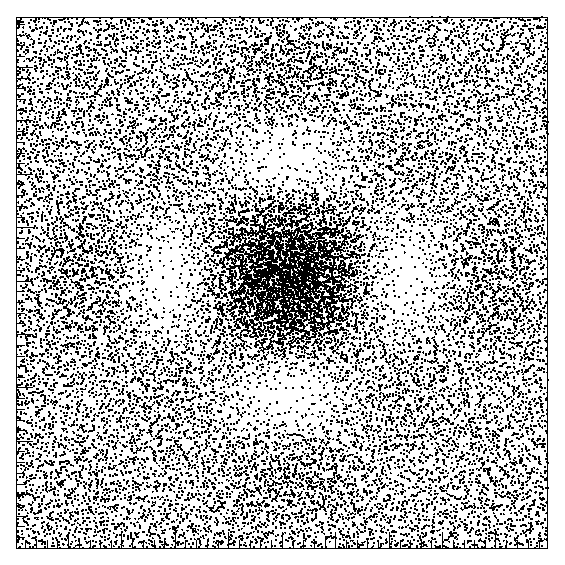
\epsfig{file=scatter.eps}} \end{center}
\caption{Example of the \protect\Rind{IGTABL} Polymarker option}
\label{SCATTER}
\end{figure}
 
\begin{figure}[p]
\begin{center}
\begin{tabular}{||c|p{12.cm}|>{\tt}r||}
\hline
\multicolumn{3}{||l||}{\bf {\tt CHOPT = 'B'} Boxes}               \\
\hline
\multicolumn{1}{||c|}{\bf {\tt PAR} index}              &
\multicolumn{1}{c|}{\bf {\tt PAR} values}               &
\multicolumn{1}{c||}{\bf default}                                 \\
\hline
 1  & Not used                                                      &         \\
 2  & Not used                                                      &         \\
 3  & {\tt XMIN} Lowest X-axis label                                &   IXMIN \\
 4  & {\tt XMAX} Highest Y-axis label                               &   IXMAX \\
 5  & {\tt YMIN} Lowest Y-axis label                                &   IYMIN \\
 6  & {\tt YMAX} Highest Y-axis label                               &   IYMAX \\
 7  & {\tt ZMIN} Lowest Z value                                     &   ZMIN  \\
 8  & {\tt ZMAX} Highest Z value                                    &   ZMAX  \\
 9  & {\tt 1000*IXMIN + IXMAX} (Useful for ZOOM)                    &   1-NX  \\
 10 & {\tt 1000*IYMIN + IYMAX} (Useful for ZOOM)                    &   1-NY  \\
\hline
\end{tabular}
\end{center}

\bigskip

\begin{center} \mbox{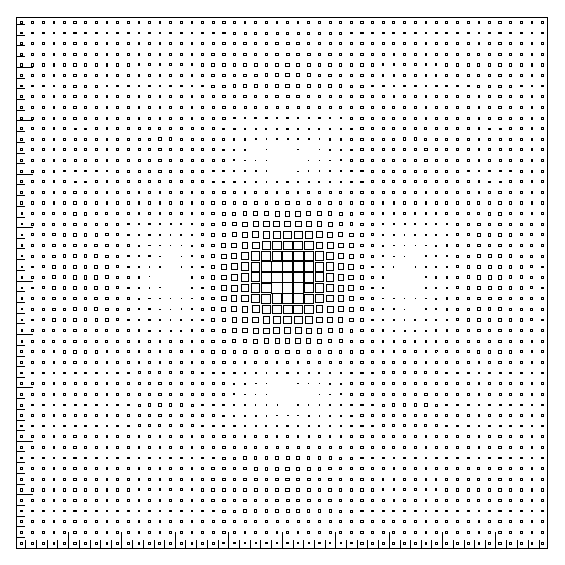
\epsfig{file=boxes.eps}} \end{center}
\caption{Example of the \protect\Rind{IGTABL} Boxes option}
\label{BOXES}
\end{figure}

\begin{figure}[p]
\begin{center}
\begin{tabular}{||c|p{12.cm}|>{\tt}r||}
\hline
\multicolumn{3}{||l||}{\bf {\tt CHOPT = 'R'} aRrows}       \\
\hline
\multicolumn{1}{||c|}{\bf {\tt PAR} index}       &
\multicolumn{1}{c|}{\bf {\tt PAR} values}        &
\multicolumn{1}{c||}{\bf default}                          \\
\hline
1  & Not used                                                       &         \\
2  & Not used                                                       &         \\
3  & XMIN Lowest X-axis label                                       &   IXMIN \\
4  & XMAX Highest Y-axis label                                      &   IXMAX \\
5  & YMIN Lowest Y-axis label                                       &   IYMIN \\
6  & YMAX Highest Y-axis label                                      &   IYMAX \\
7  & ZMIN Lowest Z value                                            &   ZMIN  \\
8  & ZMAX Highest Z value                                           &   ZMAX  \\
9  & 1000*IXMIN + IXMAX (Useful for ZOOM)                           &   1-NX  \\
10 & 1000*IYMIN + IYMAX (Useful for ZOOM)                           &   1-NY  \\
\hline
\end{tabular}
\end{center}

\bigskip

\begin{center} \mbox{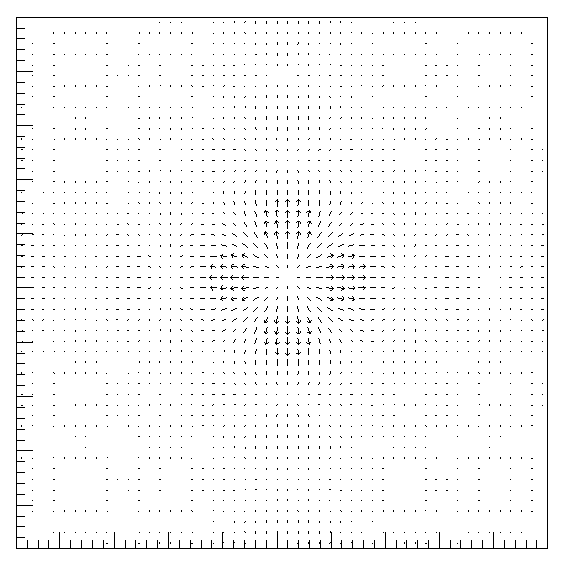
\epsfig{file=arrows.eps}} \end{center}
\caption{Example of the \protect\Rind{IGTABL} aRrows option}
\label{ARROWS}
\end{figure}

\begin{figure}[p]
\begin{center}
\begin{tabular}{||c|p{12.cm}|>{\tt}r||}
\hline
\multicolumn{3}{||l||}{\bf {\tt CHOPT = 'C'} Contour plot}     \\
\hline
\multicolumn{1}{||c|}{\bf {\tt PAR} index}           &
\multicolumn{1}{c|}{\bf {\tt PAR} values}            &
\multicolumn{1}{c||}{\bf default}                              \\
\hline
1    & Nlevel (min=2 max=50)                                        &   20.   \\
2    & 0 use colour to distinguish contours. Line type used is 1.   &    0.   \\
     & 1.XXX use line style to distinguish contours.
       Colour index used is \Lit{XXX}.                              &         \\
     & 2.XXX line style and colour are the same for all contours.   &         \\
     & Colour index used is \Lit{XXX}.                              &         \\
3    & XMIN Lowest X-axis label                                     &   IXMIN \\
4    & XMAX Highest Y-axis label                                    &   IXMAX \\
5    & YMIN Lowest Y-axis label                                     &   IYMIN \\
6    & YMAX Highest Y-axis label                                    &   IYMAX \\
7    & ZMIN Lowest Z value                                          &   ZMIN  \\
8    & ZMAX Highest Z value                                         &   ZMAX  \\
9    & 1000*IXMIN + IXMAX (Useful for ZOOM)                         &   1-NX  \\
10   & 1000*IYMIN + IYMAX (Useful for ZOOM)                         &   1-NY  \\
\hline
\end{tabular}
\end{center}

\bigskip

\begin{center} \mbox{\epsfig{file=contour.eps}} \end{center}
\caption{Example of the \protect\Rind{IGTABL} Contour option}
\label{CONTOUR}
\end{figure}

\begin{figure}[p]
\begin{center}
\begin{tabular}{||c|p{12.cm}|>{\tt}r||}
\hline
\multicolumn{3}{||l||}{\bf {\tt CHOPT = 'COL'} COLour plot}    \\
\hline
\multicolumn{1}{||c|}{\bf {\tt PAR} index}           &
\multicolumn{1}{c|}{\bf {\tt PAR} values}            &
\multicolumn{1}{c||}{\bf default}                              \\
\hline
1  & 0 use the standard 8 colours                                   &   0.    \\
2  & ...                                                            &         \\
3  & XMIN Lowest X-axis label                                       &   IXMIN \\
4  & XMAX Highest Y-axis label                                      &   IXMAX \\
5  & YMIN Lowest Y-axis label                                       &   IYMIN \\
6  & YMAX Highest Y-axis label                                      &   IYMAX \\
7  & ZMIN Lowest Z value                                            &   ZMIN  \\
8  & ZMAX Highest Z value                                           &   ZMAX  \\
9  & 1000*IXMIN + IXMAX (Useful for ZOOM)                           &   1-NX  \\
10 & 1000*IYMIN + IYMAX (Useful for ZOOM)                           &   1-NY  \\
\hline
\end{tabular}
\end{center}
\index{colour!matrix drawing}

\bigskip

\begin{center} \mbox{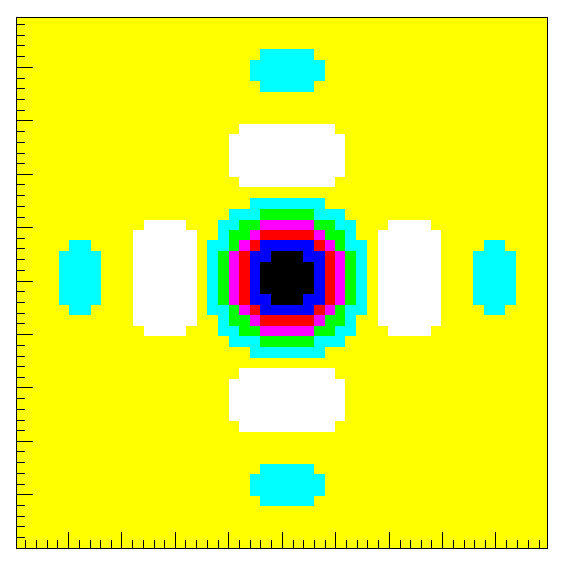
\epsfig{file=colour.eps}} \end{center}
\caption{Example of the \protect\Rind{IGTABL} COLour option}
\label{COLOUR}
\end{figure}

\begin{figure}[p]
\begin{center}
\begin{tabular}{||c|p{12.cm}|>{\tt}r||}
\hline
\multicolumn{3}{||l||}{\bf {\tt CHOPT = 'T'} Text}             \\
\hline
\multicolumn{1}{||c|}{\bf {\tt PAR} index}           &
\multicolumn{1}{c|}{\bf {\tt PAR} values}            &
\multicolumn{1}{c||}{\bf default}                              \\
\hline
1  & Text font                                                      &   1.    \\
2  & Text Precision                                                 &   0.    \\
3  & XMIN Lowest X-axis label                                       &   IXMIN \\
4  & XMAX Highest Y-axis label                                      &   IXMAX \\
5  & YMIN Lowest Y-axis label                                       &   IYMIN \\
6  & YMAX Highest Y-axis label                                      &   IYMAX \\
7  & ZMIN Lowest Z value                                            &   ZMIN  \\
8  & ZMAX Highest Z value                                           &   ZMAX  \\
9  & 1000*IXMIN + IXMAX (Useful for ZOOM)                           &   1-NX  \\
10 & 1000*IYMIN + IYMAX (Useful for ZOOM)                           &   1-NY  \\
\hline
\end{tabular}
\end{center}

\bigskip

\begin{center} \mbox{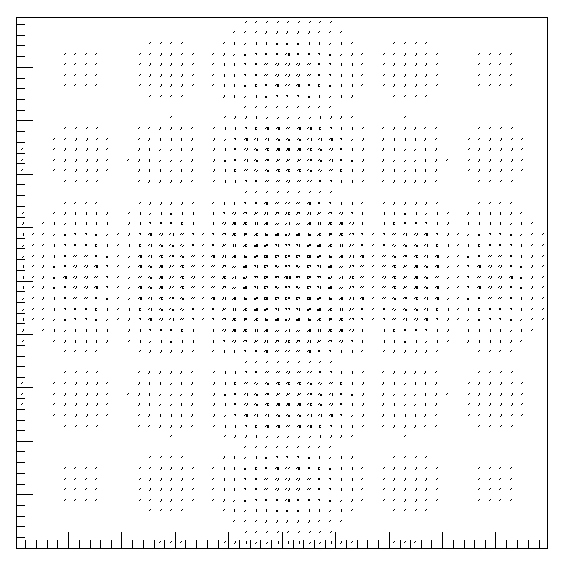
\epsfig{file=tabt.eps}} \end{center}
\caption{Example of the \protect\Rind{IGTABL} Text option}
\label{TABT}
\end{figure}

\begin{figure}[p]
\begin{center}
\begin{tabular}{||c|p{12.cm}|>{\tt}r||}
\hline
\multicolumn{3}{||l||}{\bf {\tt CHOPT = 'K'} character}     \\
\hline
\multicolumn{1}{||c|}{\bf {\tt PAR} index}        &
\multicolumn{1}{c|}{\bf {\tt PAR} values}         &
\multicolumn{1}{c||}{\bf default}                           \\
\hline
1  & Text font                                                      &   1.    \\
2  & Text Precision                                                 &   0.    \\
3  & XMIN Lowest X-axis label                                       &   IXMIN \\
4  & XMAX Highest Y-axis label                                      &   IXMAX \\
5  & YMIN Lowest Y-axis label                                       &   IYMIN \\
6  & YMAX Highest Y-axis label                                      &   IYMAX \\
7  & ZMIN Lowest Z value                                            &   ZMIN  \\
8  & ZMAX Highest Z value                                           &   ZMAX  \\
9  & 1000*IXMIN + IXMAX (Useful for ZOOM)                           &   1-NX  \\
10 & 1000*IYMIN + IYMAX (Useful for ZOOM)                           &   1-NY  \\
\hline
\end{tabular}
\end{center}

\bigskip

\begin{center} \mbox{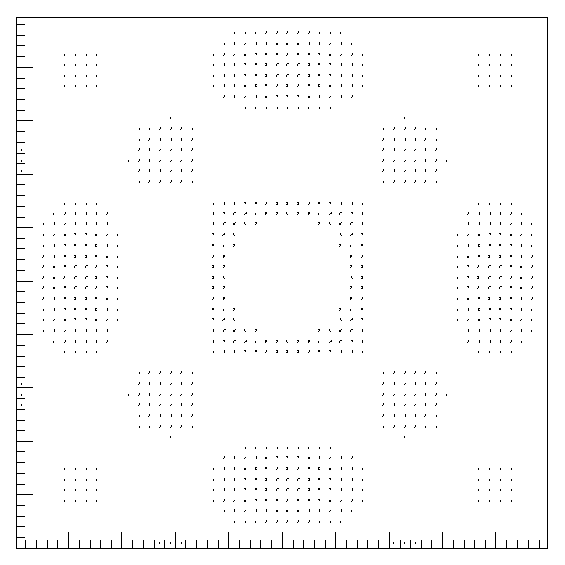
\epsfig{file=tabk.eps}} \end{center}
\caption{Example of the \protect\Rind{IGTABL} character \protect\Lit{K} option}
\label{TABK}
\end{figure}

\begin{table}[p]
\begin{center}
\begin{tabular}{||c|p{12.cm}|>{\tt}r||}
\hline
\multicolumn{3}{||l||}
{\bf {\tt CHOPT = 'L'} Lego (mode 0)}                                         \\
\multicolumn{3}{||l||}
{\bf {\tt CHOPT = 'LB'} Lego with BARO and BARW}                              \\
\multicolumn{3}{||l||}
{\bf {\tt CHOPT = 'L1'} Lego with colours (mode 1)}                           \\
\multicolumn{3}{||l||}
{\bf {\tt CHOPT = 'L2'} Lego with colours (mode 2)}                           \\
\hline
\multicolumn{3}{||l||}
{\bf {\tt CHOPT = 'S'} Surface (mode 0)}                                      \\
\multicolumn{3}{||l||}
{\bf {\tt CHOPT = 'S1'} Surface with colours (mode 1)}                        \\
\multicolumn{3}{||l||}
{\bf {\tt CHOPT = 'S2'} Surface with colours (mode 2)}                        \\
\multicolumn{3}{||l||}
{\bf {\tt CHOPT = 'S3'} Surface with contour plot on top (mode 3)}            \\
\multicolumn{3}{||l||}
{\bf {\tt CHOPT = 'S4'} Surface with Gouraud shading (mode 4)}                \\
\hline
\multicolumn{3}{||l||}
{\bf {\tt CHOPT = 'CYL'} Cylindrical for lego and surface}                    \\
\multicolumn{3}{||l||}
{\bf {\tt CHOPT = 'SPH'} Spherical for lego and surface}                      \\
\multicolumn{3}{||l||}
{\bf {\tt CHOPT = 'PSD'} Pseudo rapidity for lego and surface}                \\
\hline
\multicolumn{1}{||c|}{\bf {\tt PAR} index}       &
\multicolumn{1}{c|}{\bf {\tt PAR} values}        &
\multicolumn{1}{c||}{\bf default}                          \\
\hline
1  & {\tt THETA}                                                    &   30.   \\
2  & {\tt PHI}                                                      &   30.   \\
3  & {\tt XMIN} Lowest X-axis label                                 &   IXMIN \\
4  & {\tt XMAX} Highest Y-axis label                                &   IXMAX \\
5  & {\tt YMIN} Lowest Y-axis label                                 &   IYMIN \\
6  & {\tt YMAX} Highest Y-axis label                                &   IYMAX \\
7  & {\tt ZMIN} Lowest Z value                                      &   ZMIN  \\
8  & {\tt ZMAX} Highest Z value                                     &   ZMAX  \\
9  & {\tt 1000*IXMIN + IXMAX} (Useful for ZOOM)                     &   1-NX  \\
10 & {\tt 1000*IYMIN + IYMAX} (Useful for ZOOM)                     &   1-NY  \\
11 & {\tt NDVX}                                                     &  510.00 \\
12 & {\tt NDVY}                                                     &  510.00 \\
13 & {\tt NDVZ}                                                     &  510.00 \\
14 & {\tt XCOL}                                                     &    1.00 \\
15 & {\tt YCOL}                                                     &    1.00 \\
16 & {\tt ZCOL}                                                     &    1.00 \\
17 & {\tt XTIC}                                                     &    0.02 \\
18 & {\tt YTIC}                                                     &    0.02 \\
19 & {\tt ZTIC}                                                     &    0.02 \\
20 & {\tt VSIZ}                                                     &    0.02 \\
21 & {\tt VFON}                                                     &    2.00 \\
22 & {\tt XVAL}                                                     &    0.02 \\
23 & {\tt YVAL}                                                     &    0.02 \\
24 & {\tt ZVAL}                                                     &    0.04 \\
25 & Palette                                                        &    0.04 \\
\hline
\end{tabular}
\end{center}
\caption{Values of the \protect\Rind{IGTABL} Lego and Surface option}
\label{tab-IGTABLS}
\end{table}

\begin{figure}[p]
\begin{center}\mbox{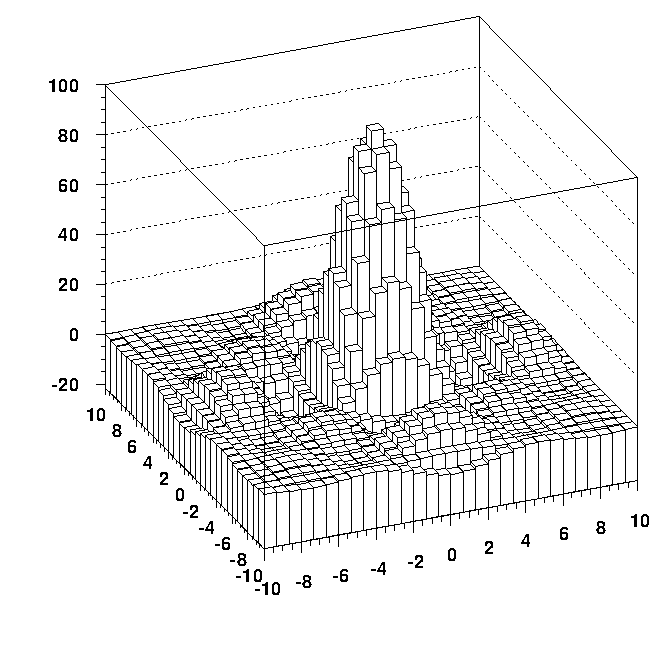
\epsfig{file=lego.eps}}\end{center}
\caption{Example of the \protect\Rind{IGTABL} Lego option}
\label{LEGO}
\begin{center}\mbox{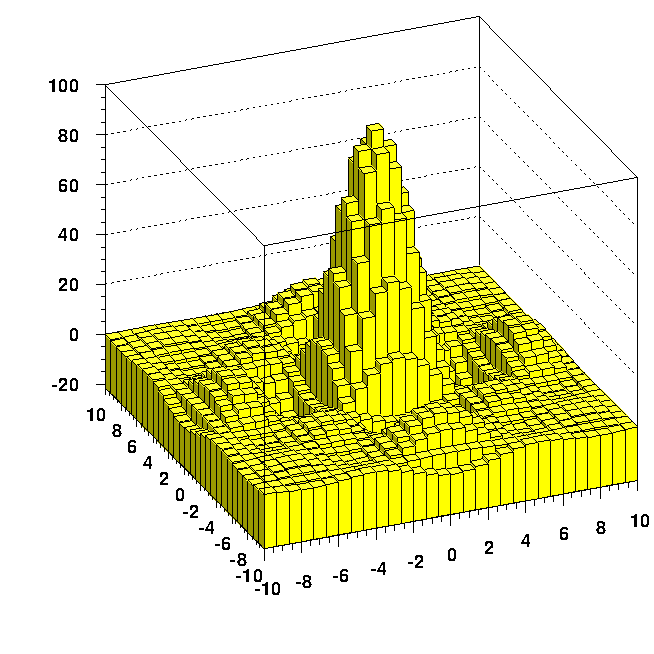
\epsfig{file=lego1.eps}}\end{center}
\caption{Example of the \protect\Rind{IGTABL} Lego \protect\Lit{L1} option}
\label{LEGO1}
\end{figure}

\begin{figure}[p]
\begin{center}\mbox{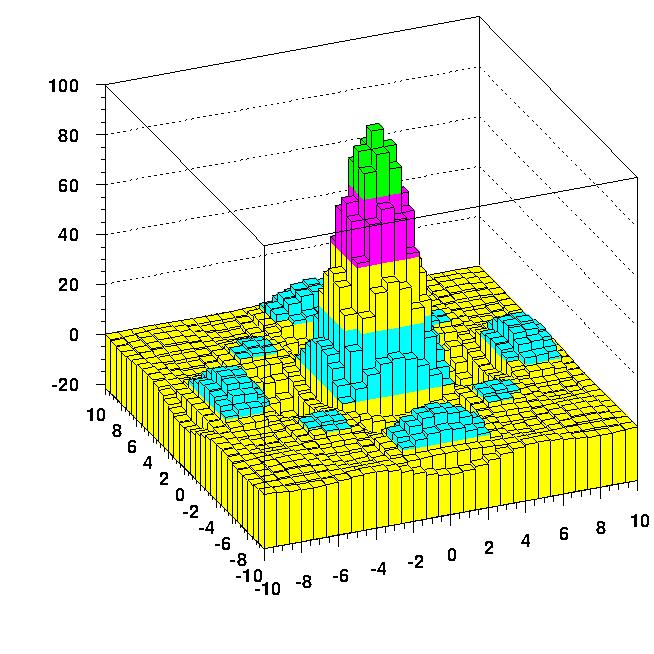
\epsfig{file=lego2.eps}}\end{center}
\caption{Example of the \protect\Rind{IGTABL} Lego \protect\Lit{L2} option}
\label{LEGO2}
\begin{center}\mbox{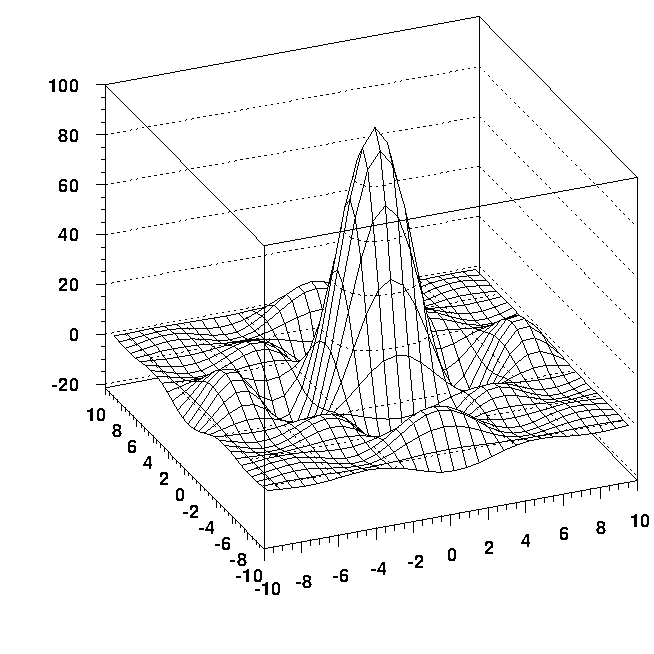
\epsfig{file=surf.eps}}\end{center}
\caption{Example of the \protect\Rind{IGTABL} Surface option}
\label{SURF}
\end{figure}

\begin{figure}[p]
\begin{center}\mbox{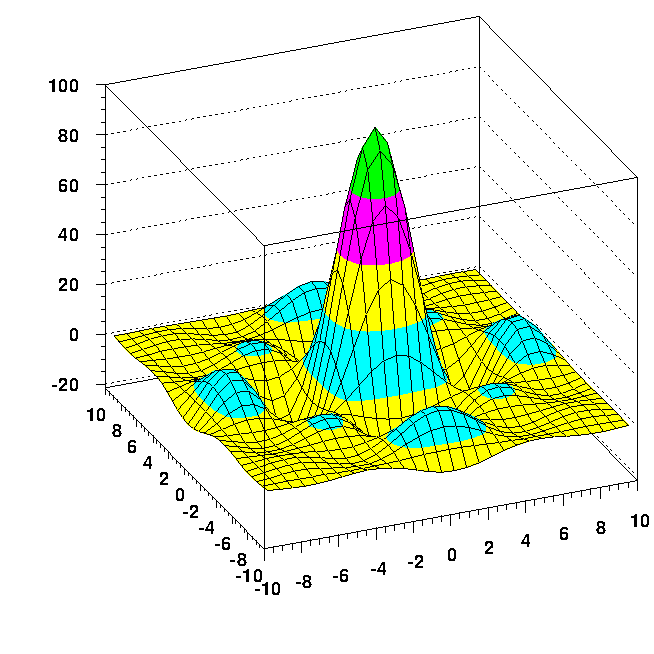
\epsfig{file=surf1.eps}}\end{center}
\caption{Example of the \protect\Rind{IGTABL} Surface \protect\Lit{S1} option}
\label{SURF1}
\begin{center}\mbox{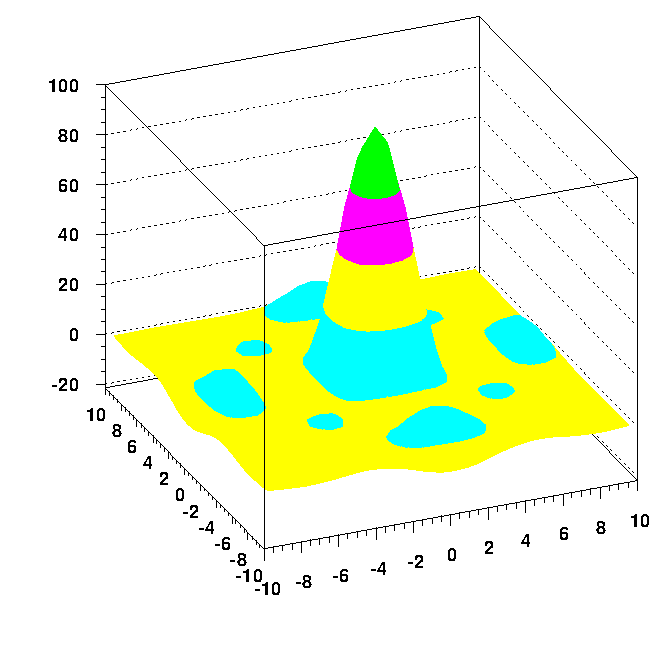
\epsfig{file=surf2.eps}}\end{center}
\caption{Example of the \protect\Rind{IGTABL} Surface \protect\Lit{S2} option}
\label{SURF2}
\end{figure}

\begin{figure}[p]
\begin{center}\mbox{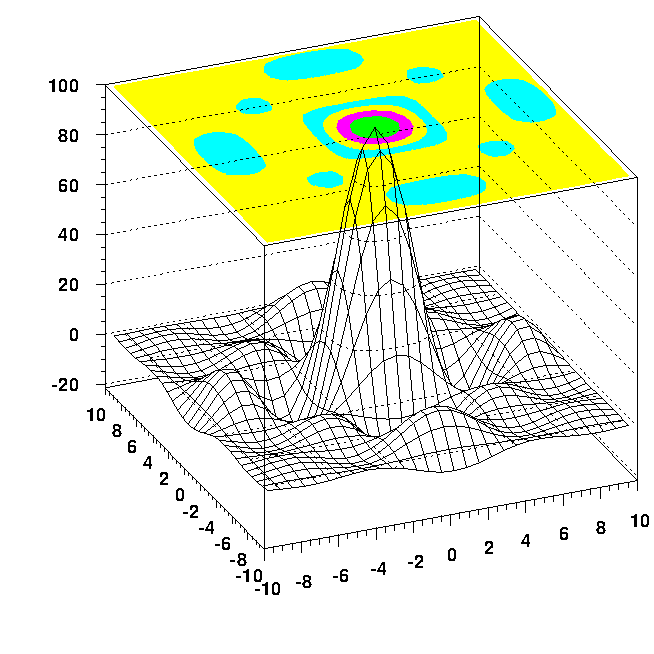
\epsfig{file=surf3.eps}}\end{center}
\caption{Example of the \protect\Rind{IGTABL} Surface \protect\Lit{S3} option}
\label{SURF3}
\begin{center}\mbox{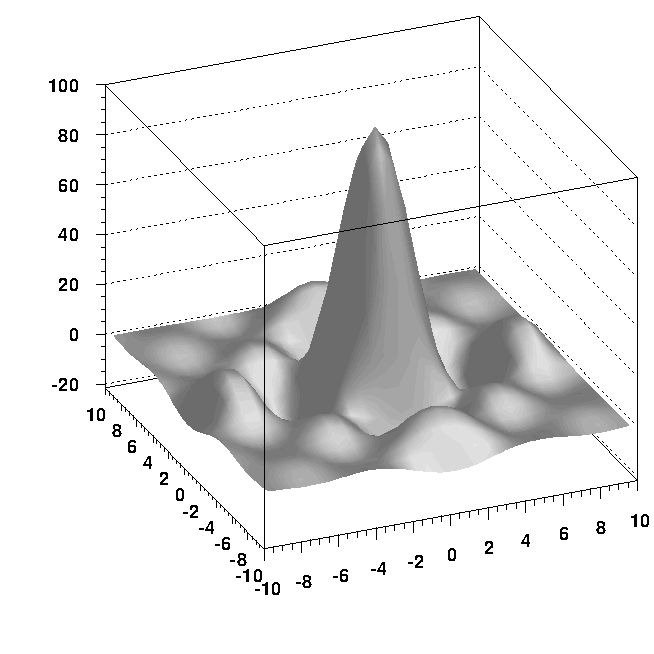
\epsfig{file=surf4.eps}}\end{center}
\caption{Example of the \protect\Rind{IGTABL} Surface \protect\Lit{S4} option}
\label{SURF4}
\end{figure}

\begin{figure}[p]
\begin{center}\mbox{\epsfig{file=surfpol.eps}}\end{center}
\caption{Example of the \protect\Rind{IGTABL} Surface \protect\Lit{SPOL} option}
\label{SPOL}
\begin{center}\mbox{\epsfig{file=surfcyl.eps}}\end{center}
\caption{Example of the \protect\Rind{IGTABL} Surface \protect\Lit{SCYL} option}
\label{SCYL}
\end{figure}

\begin{figure}[p]
\begin{center}\mbox{\epsfig{file=surfsph.eps}}\end{center}
\caption{Example of the \protect\Rind{IGTABL} Surface \protect\Lit{SSPH} option}
\label{SSPH}
\begin{center}\mbox{\epsfig{file=surfpsd.eps}}\end{center}
\caption{Example of the \protect\Rind{IGTABL} Surface \protect\Lit{SPSD} option}
\label{SPSD}
\end{figure}

Note that the options \Lit{POL}, \Lit{CYL}, \Lit{SPH}, and \Lit{PSD} can be
used together with any lego or surface options.
\clearpage

\begin{Tabhere}
\begin{tabularx}{\textwidth}{||c|X||}
\hline
 \Lit{CHOPT} &                Description                                           \\
\hline
  'H'  & Data are compacted as in \HPLOT.                                     \\
\hline
  'GX' & loG on X coordinates. A log \WC~must be defined before.              \\
\hline
  'GY' & loG on Y coordinates. A log \WC~must be defined before.              \\
\hline
  'GZ' & loG on Z coordinates.                                                \\
\hline
  'A'  & 2nd vertical axis (legos and Surfaces only)                          \\
       & axis (for the 2D representations).                                   \\
\hline
  '+'  & For stacked histograms (legos).                                      \\
\hline
  'Z'  & Allows to display the Z scale.                                       \\
\hline
\end{tabularx}
\caption{Other options for \protect\Rind{IGTABL}}
\label{tab-IGTABL}
\end{Tabhere}

\begin{XMPt}{Example of stacked lego plots drawing (see result on figure 
\ref{STACK})}
      program stack 
      parameter (nx=10,ny=10)
      parameter (npar=25)
      dimension v1(nx,ny),v2(nx,ny),v3(nx,ny)
      dimension par(npar)
      call vzero(par,npar)
      par(1)  = 30.
      par(2)  = 23.
      par(3)  = -10.
      par(4)  = 10.
      par(5)  = -10
      par(6)  = 10.
      par(9)  = 1000. + nx
      par(10) = 1000. + ny
      par(11) = 510.
      par(12) = 510.
      par(13) = 510.
      par(14) = 1.
      par(15) = 1.
      par(16) = 1.
      par(20) = 0.05
      par(21) = -61.
      par(22) = .1
      par(23) = .15
      par(24) = .1
*
*              Matrices filling
*
      do i=1,nx
         do j=1,ny
            v1(i,j)=float(i)
            v2(i,j)=float(i+j)
            v3(i,j)=float(j)
         enddo
      enddo
*
*              Stack drawing
*
      call start('stack',9.,9.)
      call igset('BARW',0.5)
      par(25) = 2.
      call igtabl(nx,ny,v1,npar,par,'+')
      par(25) = 5.
      call igtabl(nx,ny,v2,npar,par,'+')
      par(25) = 3.
      call igtabl(nx,ny,v3,npar,par,'LB1A')
      call igterm
      call finish
*
      end
\end{XMPt}

\begin{Fighere}
\begin{center}\mbox{\epsfig{file=stack.eps}}\end{center}
\caption{Example of stacked lego plots}
\label{STACK}
\end{Fighere}
\clearpage

\Filename{H2Drawingapiechart}
\section{Drawing a pie chart}
\index{pie chart drawing}
\Shubr{IGPIE}{(X0,Y0,RADIUS,N,VALUES,CHOPT,IAO,IAS,IAC)}
\Action
This routine draws a graph in form of a pie chart.
\Pdesc
\begin{DLtt}{1234567}
\item[X0]     X coordinate of the center of the pie chart.
\item[Y0]     Y coordinate of the center of the pie chart.
\item[RADIUS] Radius of the pie chart.
\item[N]      Number of entries in the array {\tt VALUES}
\item[VALUES] Array of dimension {\tt N} containing the values determining
              the size of the slices in the pie.
\item[CHOPT]  Character variable specifying the combination of options
              desired:
\begin{DLtt}{12345}
\item['C'] Colours array is present.
\item['L'] Alphanumeric labels are required (see section \ref{IGLBL}).
\item['O'] Offset array is present.
\item['N'] The label of each slice will be the corresponding numeric value in
           array {\tt VALUES}.
\item['P'] The label of each slice will be in expressed in percentage.
\item['S'] Style array is present.
\item['H'] Force the labels size to be the current character height. Without
           this option the labels size is computed automatically.
\item['R'] Draw the labels aligned on the radius of each slice.
\end{DLtt}
\item[IAO] Array of dimension {\tt N} containing offsets of the corresponding
           slice in percentage of the radius.
\item[IAS] Array of dimension {\tt N} containing the interior style index for
           every slice.
\item[IAC] Array of dimension {\tt N} containing the colour index for every
           slice.
\end{DLtt}
\newpage

\begin{XMPt}{Example of {\tt PIE CHART} drawing (see result on figure \ref{PIE}}
      program  pie 
      dimension v(8),iao(8),ias(8)
      data v /1.,1.8,2.9,1.,1.8,2.9,1.,1.8/
      data iao /0,0,0,20,0,0,20,0/
      data ias /205,295,245,244,254,245,244,245/
      call start('pie',12.,9.)
      call isclip(0)
      call igbox(0.,12.,0.,9.)
      call igset('BORD',1.)
      call igpie(3.,6.,2.,8,v,'OSN',iao,ias,0)
      call igpie(9.,6.,2.,8,v,'OSP',iao,ias,0)
      call igset('TXAL',23.)
      call igset('CHHE',0.3)
      call itx(3.,3.,'CHOPT = ''OSN''')
      call itx(9.,3.,'CHOPT = ''OSP''')
      call itx(6.,2.,'IAO = 0,0,0,20,0,0,20,0')
      call itx(6.,1.,'IAS = 205,295,245,244,254,245,244,245')
      call finish
      end
\end{XMPt}

\begin{Fighere}
\begin{center}
\mbox{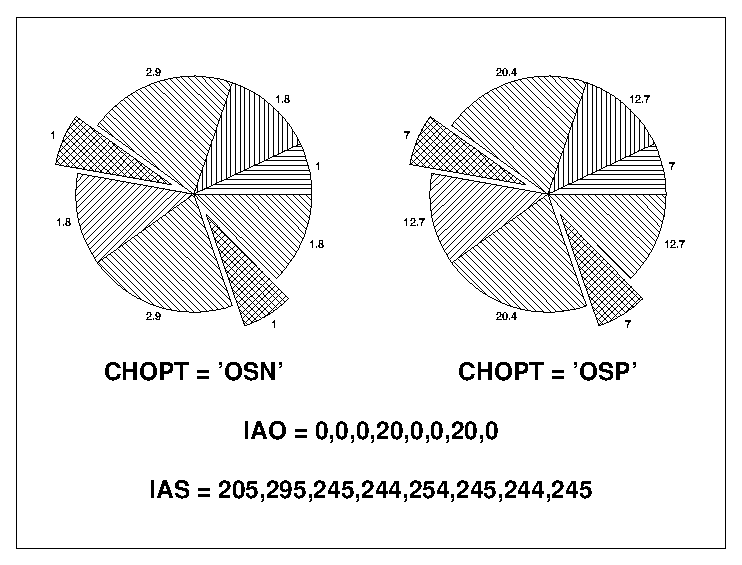
\epsfig{file=pie.eps,height=9cm}}
\end{center}
\caption{Examples of \protect\Rind{IGPIE}}
\label{PIE}
\end{Fighere}
\clearpage
 
\Filename{H2Drawingaxes}
\section{Drawing axes}
\index{axis drawing}
\Shubr{IGAXIS}{(X0,X1,Y0,Y1,WMIN,WMAX,NDIV,CHOPT)}
\Action
This routines allows the user to draw axes on a picture.
\Pdesc
\begin{DLtt}{1234567}
\item[X0]   X coordinate of the origin of the axis in \WC~space.
\item[X1]   X coordinate of the end of the axis in \WC~space.
\item[Y0]   Y coordinate of the origin of the axis in \WC~space.
\item[Y1]   Y coordinate of the end of the axis in \WC~space.
\item[WMIN] Lowest value for the tick mark labels written on the axis.
\item[WMAX] Highest value for the tick mark labels written on the axis.
\item[NDIV] Number of divisions. calculated according to the following
            convention:
\begin{DLtt}{123}
\item[NDIV = N1 + 100*N2 + 10000*N3] where,
\item[N1] Number of primary divisions.
\item[N2] Number of second order divisions.
\item[N3] Number of third order divisions.
\end{DLtt}
Examples:
\begin{DLtt}{1234567}
\item[NDIV=0] No tick marks.
\item[NDIV=2] produces 2 divisions with one tick mark in the middle of the axis.
\end{DLtt}
Note that, in case numeric labels are requested, {\tt N1} indicates the maximum
number of primary divisions. An appropriate algorithm calculates a number of
primary divisions less or equal to N1, in order to obtain ``reasonable'' labels.
Option {\tt'N'} in {\tt CHOPT} forces {\tt N1} to be used as the {\bf exact}
number of primary divisions.
\item[CHOPT] Character variable specifying the combinations of options desired.
\par {\bf General options}
\begin{DLtt}{12345}
\item['G'] LoGarithmic scale, default is linear.
\item['B'] Blank axis, i.e. the base line constituting the axis is not drawn.
           However tick marks and labels are drawn. Useful when superimposing
           two axes.
\item['A'] An arrow is drawn at the end of the axis (position {\tt WMAX}).
\item['N'] N1 will be used as exact number of divisions.
\end{DLtt}
 
{\bf Orientation of the tick marks on the axis }
\index{axis!tick marks!orientation}
 
Tick marks are normally drawn on the positive side of the axis. However, if the
axis is vertical, i.e. if {\tt X0=X1}, then they are drawn on the ``negative''
side. Their orientation can be selected by {\tt CHOPT}.
\begin{DLtt}{12345}
\item['+'] Tick marks are drawn on the positive side of the axis (default).
\item['-'] Tick marks are drawn on the negative side of the axis.
\end{DLtt}
Specifying {\tt'+-'} will draw tick marks on {\bf both} sides of the axis.
 
{\bf Orientation of tick marks and labels in the working space }
\index{axis!tick marks!orientation}
\index{axis!labels!orientation}
 
Tick marks are normally drawn orthogonal to the axis.
However, in case of an oblique axis, they can be drawn vertically.
\begin{DLtt}{12345}
\item['V'] Tick marks are drawn Vertically (default is perpendicular to axis).
\end{DLtt}
 
\newpage
{\bf Labeling an axis }
\index{axis!labeling}
 
An axis is normally labeled, unless specified otherwise:
\begin{DLtt}{12345}
\item['U'] Unlabeled axis (default is labeled).
\end{DLtt}
 
{\bf Position of labels on an axis }
\index{axis!labels!position}
 
Labels are normally drawn on the side opposite to the tick marks,
unless specified otherwise:
\begin{DLtt}{12345}
\item['='] Labels are drawn on the same side as the tick marks.
\end{DLtt}
 
{\bf Orientation of labels on an axis. }
\index{axis!labels!orientation}
 
Labels are normally drawn parallel to the axis.
 
However if the axis is vertical, i.e.
if {\tt X0=X1}, then the labels are drawn
orthogonally. If the axis is horizontal, i.e. if {\tt Y0=Y1}, then the
labels are Parallel to the axis:
\begin{DLtt}{12345}
\item['P'] Labels are drawn Parallel to the axis
\item['O'] Labels are drawn Orthogonal to the axis.
\end{DLtt}
 
{\bf Position of labels with respect to the tick marks. }
\index{axis!labels!position}
 
Labels are centered on tick marks. However,
if the axis is vertical ({\tt X0=X1}), then they are right adjusted.
\begin{DLtt}{12345}
\item['R'] Labels are Right adjusted on a tick mark.
\item['L'] Labels are Left adjusted on a tick mark.
\item['C'] Labels are centered on tick a mark. (default)
\end{DLtt}
 
{\bf Direction of labels }
\index{axis!labels!direction}
 
The default writing direction of labels is from {\bf left to right}.
\begin{DLtt}{12345}
\item['Y'] Writing direction is {\bf downwards}.
\end{DLtt}
 
{\bf Format of labels }
\index{axis!labels!format}
 
Training blanks in the label strings are stripped, and then the label is
correctly aligned. If the last character of the string is a dot {\tt'.'},
it is also stripped by default.
\begin{DLtt}{12345}
\item['.'] The dot at the end of a string is mandatory.
\end{DLtt}
 
{\bf Type of labels }
\index{axis!labels!type}
\index{axis!labels!alphanumeric}
 
Labels are by default numeric.
\begin{DLtt}{12345}
\item['T'] The labels are alphanumeric text strings. In this case 12 default
           values are provided, namely the 3-character abbreviations of the
           names of the months: {\tt'JAN'}, {\tt'FEB'}, {\tt'MAR'},\ldots.
           These values can be modified by calling the routine \Rind{IGLBL}
           (see section \ref{IGLBL}).
\end{DLtt}
 
{\bf Optional grid }
\index{grid|see{axis grid}}
 
An optional grid (cross-wires) can be drawn as a prolongation of the primary
tick marks.
\begin{DLtt}{12345}
\item['W'] Draw cross-wires at the position of the primary tick marks.
           The length of the grid can be defined, in \WC, with the
           \Rind{IGSET} parameter \Sind{AWLN}. The current line type
           is used to draw the grid.
\end{DLtt}
 
{\bf Intrinsic parameters }
\index{axis!intrinsic parameters}
 
The default values for \HIGZ~intrinsic parameter settings are shown below
expressed as a percentage of the length of the axis (\WC):
\begin{DL}{\bf Characters height for labels:M}
\item[Primary tick marks:] 3.0 \%
\item[Secondary tick marks:]1.5 \%
\item[Third order tick marks:].75 \%
\item[Length of the arrow:]3.0 \%
\item[Width of the arrow:].75 \%
\item[Characters height for labels:] 2.0 \%
\item[Characters spacing:] 40\% of the character height
\item[Labels offset:] 4.0 \%
\end{DL}
 
The size of the secondary tick marks is always 50\% of the primary ones. The
size of the third order tick marks is always 50\% of the secondary ones.
 
These values can be changed by calls to routine \Rind{IGSET}. The default value
is used {\bf unless } the corresponding option is selected by {\tt CHOPT}:
\begin{DLtt}{12345}
\item['D'] The distance between the labels and the axis (the offset) is given by
           the preceding call to \Rind{IGSET} with the parameter \Sind{LAOF}.
\item['H'] The size (height) of the labels is given by the preceding call to
           \Rind{IGSET} with the parameter \Sind{LASI}.
\item['S'] The size of the tick marks is given by the preceding call to
           \Rind{IGSET} with the parameter \Sind{TMSI}.
\end{DLtt}
\end{DLtt}
 
\subsection{Control of Alphanumeric labels}
\index{axis!labels!alphanumeric}
\Shubr{IGLBL}{(NLBL,CHLBL)}
\Action
This routine must be called to alter the values of the alphanumeric labels used
in \Rind{IGAXIS}.
\Pdesc
\begin{DLtt}{1234567}
\item[NLBL] Number of alphanumeric labels specified in array {\tt CHLBL}.
            The number of labels is limited to 50.
\item[CHLBL] {\tt CHARACTER} array containing the new values for the
             alphanumeric labels. The maximal length of each label is 32
             characters.
\end{DLtt}

\newpage

\begin{XMPt}{Example of {\tt AXIS} drawing (see result on figure \ref{AXIS})}
      program axis 
      call start('axis',12.,12.)
      call igbox(0.,12.,0.,12.)
      call igaxis (1.,11.,1.,1.,0.,100.,510,'A')
      call igaxis (1.,11.,3.,3.,1.,10000.,510,'G')
      call igaxis (1.,11.,5.,5.,0.,12.,11,'NATY')
      call igaxis (1.,11.,6.,6.,-100.,0.,510,'A')
      call igaxis (11.,1.,7.,7.,-100.,0.,810,'A+-')
      call igaxis (1.,11.,8.,11.,0.,1234567.,615,'A')
      call igaxis (6.,11.,8.5,8.5,-3.14,0.,50505,'AN')
      call finish
      end
\end{XMPt}
 
\begin{Fighere}
\begin{center}
\mbox{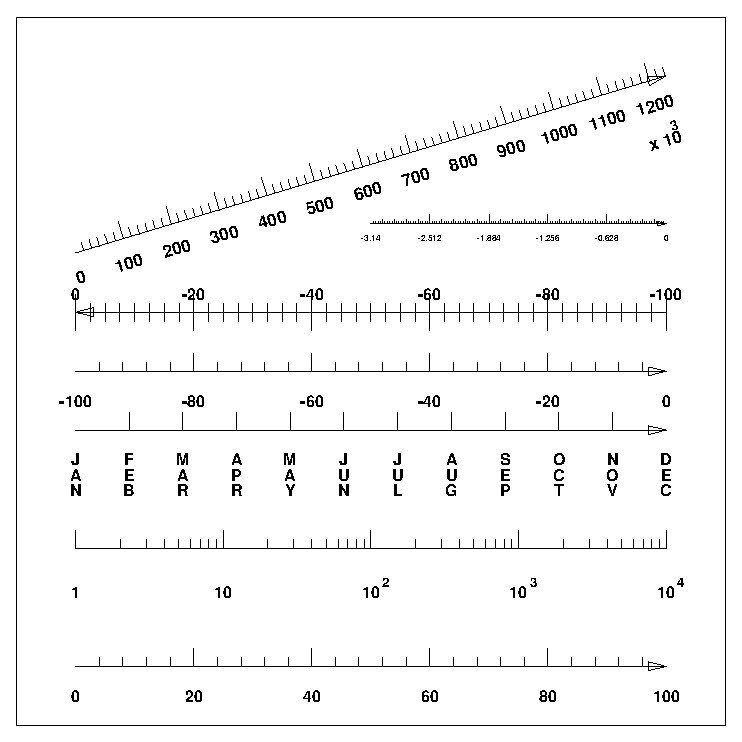
\epsfig{file=axis.eps,height=12cm}}
\end{center}
\caption{Examples of \protect\Rind{IGAXIS}}
\label{AXIS}
\end{Fighere}
 
\newpage

\Filename{H2Drawingsoftwarecharacters}
\section{Drawing software characters}
\index{text!software characters}
\Shubr{IGTEXT}{(X,Y,CHARS,SIZE,ANGLE,CHOPT)}
\Action
This routine draws a software character text, independently from \UGP{} used by
\HIGZ. \Rind{IGTEXT} can produce over 300 different graphic signs.
The way in which software characters are defined is via a string of valid
\FORTRAN{} characters, intermixed by other valid \FORTRAN{} characters, acting as
``escape'' characters \index{character!escape} (e.g. a change of
alphabet, upper or lower case). The string is interpreted by \Rind{IGTEXT} and
the resulting characters are defined according to the figure~\ref{SOFTTEXT},
which shows the list of available software characters. This routine allows the
user to mix different types of characters (roman, greek, special, upper and
lower case, sub and superscript). There are a total of 10 control characters.
\Pdesc
\begin{DLtt}{1234567}
\item[X] x coordinate in \WC space.
\item[Y] y coordinate in \WC space.
\item[CHARS] {\tt CHARACTER} variable containing the text
to be displayed.
\item[SIZE] Size of the text in \WC space.
\item[ANGLE] Inclination angle of the text inclination in degrees.
\item[CHOPT] {\tt CHARACTER} variable specifying the text alignment:
\begin{DLtt}{12345}
\item['L'] The text is Left adjusted starting at the point {\tt(X,Y)}.
\item['C'] The text is Centered around the the point {\tt(X,Y)}.
\item['R'] The text is Right adjusted ending at the point {\tt(X,Y)}.
\item['S'] The text size (length) is returned in \Lit{ANGLE}.
\end{DLtt}
Note that it is not possible to align vertically the text produce by
\Rind{IGTEXT}. The way to align vertically software text is to use \Rind{ITX}
with the font {\tt 0} and precision {\tt 2} (see \Rind{ISTXFP}).
\end{DLtt}
\index{lower case letters}
\index{upper case letters}
\index{Greek letters}
\index{superscript}
\index{subscript}
\index{backspace}
\index{termination character}
\index{special symbols}
\label{ESCCHAR}
\begin{tabular}{||c|p{7cm}||c|p{7cm}||}
\hline
\multicolumn{4}{|c|}{\bf List of escape characters and their meaning}      \\
\hline
 $<$  & go to lower case                 & $>$  & go to upper case (default) \\
\hline
 \lsb & go to greek (Roman = default)    & \rsb & end of greek               \\
\hline
 "    & go to special symbols            & \#   & end of special symbols     \\
\hline
$\uparrow$  & go to superscript         & ?    & go to subscript            \\
\hline
 !    & go to normal level of script     & \&   & backspace one character    \\
\hline
 \$   & termination character (optional) &      &                            \\
\hline
\end{tabular}
\par
Note that characters can be also entered directly in lower case or upper case
instead of using the control characters {\tt <} and {\tt >}.
\par
The boldface characters may be simulated by setting the
attributes '\Sind{PASS}' and '\Sind{CSHI}' with \Rind{IGSET}.
The meaning of these attributes is the
following: Every stroke used to display the character is repeated
\Sind{PASS} times, at a distance (in percentage of the character height)
given by \Sind{CSHI}.

\begin{figure}[p]
\begin{center}
\mbox{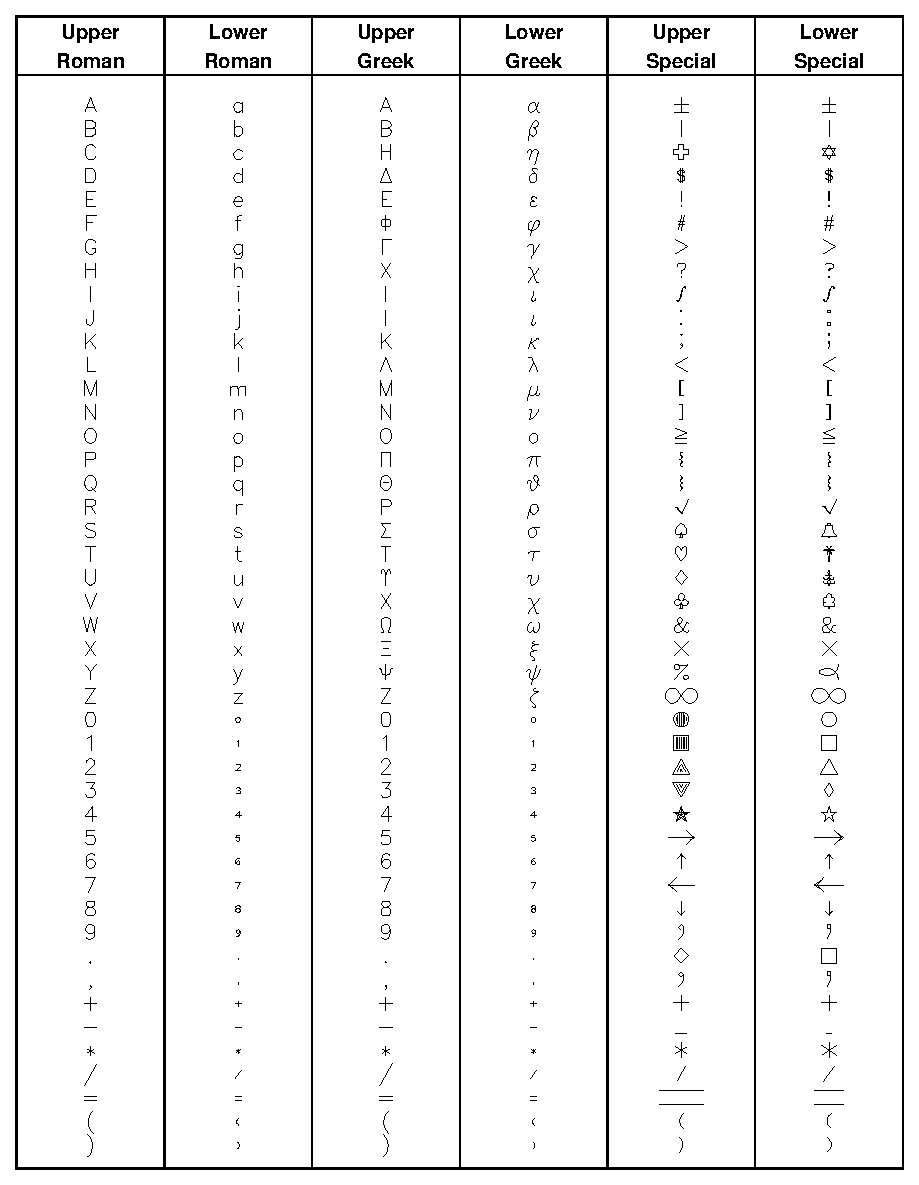
\epsfig{file=softtext.eps}}
\end{center}
\caption{Characters available in \protect\Rind{IGTEXT}}
\label{SOFTTEXT}
\end{figure}
\clearpage 

\Filename{H2Settingattributes}
\section{Setting attributes}
\index{attributes!setting}
\Shubr{IGSET}{(CHNAME,VAL)}
\Action
Routine used to set the value of attributes related to
primitives and/or macroprimitives. 
The first parameter is
the mnemonic name of the parameter, the second is the value to be assigned.
Note that all the
basic primitives attributes can also be set with this routine.
\begin{DLtt}{1234567}
\item[CHNAME] Character variable specifying the name of
the parameter to be set (type {\tt CHARACTER*4}). This is an UPPERCASE
character string.
\item[VAL] {\bf Floating point} value of the parameter (must be specified
as a {\tt REAL} number).\\
A value of {\tt0.0} indicates that the parameter value must
be reset to its default value.
\end{DLtt}

\begin{table}[p]
\index{fill area!interior style}
\index{fill area!style index}
\index{fill area!colour index}
\index{polyline!type}
\index{polyline!width}
\index{polyline!colour index}
\index{polymarker!type}
\index{polymarker!scale factor}
\index{polymarker!colour index}
\index{text!colour index}
\index{text!alignment}
\index{text!character height}
\index{text!angle}
\index{text!font}
\index{text!precision}
\index{text!width}
\index{axis!tick marks size}
\index{axis!labels size}
\index{axis!labels offset}
\index{box!border}
\index{arc!border}
\index{automatic naming of pictures}
\index{colour!map}
\begin{tabularx}{\textwidth}{|c|X|}
\hline
\multicolumn{1}{|c|}{\tt CHNAME} & \multicolumn{1}{c|}{\tt VAL} \\
\hline
'\Sind{FAIS}'     & Fill Area Interior Style (0.,1.,2.,3.). See \Rind{ISFAIS} \\
'\Sind{FASI}'     & Fill Area Style Index. See \Rind{ISFASI}                  \\
'\Sind{LTYP}'     & Line TYPe. See \Rind{ISLN}                                \\
'\Sind{BASL}'     & BAsic Segment Length. See \Rind{ISLN}                     \\
'\Sind{LWID}'     & Line WIDth. See \Rind{ISLWSC}                             \\
'\Sind{MTYP}'     & Marker TYPe. See \Rind{ISMK}                              \\
'\Sind{MSCF}'     & Marker SCale Factor. See \Rind{ISMKSC}                    \\
'\Sind{PLCI}'     & PolyLine Colour Index. See \Rind{ISPLCI}                  \\
'\Sind{PMCI}'     & PolyMarker Colour Index. See \Rind{ISPMCI}                \\
'\Sind{FACI}'     & Fill Area Colour Index. See \Rind{ISFACI}                 \\
'\Sind{TXCI}'     & TeXt Colour Index. See \Rind{ISTXCI}                      \\
'\Sind{TXAL}'     & 10*(horizontal alignment) + (vertical alignment).
                    See \Rind{ISTXAL}                                         \\
'\Sind{CHHE}'     & CHaracter HEight. See \Rind{ISCHH}                        \\
'\Sind{TANG}'     & Text ANGle (used to calculate the Character up vector).
                    See \Rind{ISCHUP}                                         \\
'\Sind{TXFP}'     & 10*(TeXt Font) + (TeXt Precision). See \Rind{ISTXFP}      \\
'\Sind{TMSI}'     & Tick Marks SIze (in \WC). See \Rind{IGAXIS}               \\
'\Sind{LASI}'     & LAbels SIze (in \WC). See \Rind{IGAXIS}                   \\
'\Sind{LAOF}'     & LAbels OFfset. See \Rind{IGAXIS}                          \\
'\Sind{AWLN}'     & Axis Wire LeNght. See \Rind{IGAXIS}                       \\
'\Sind{PASS}'     & Text width (given by number of {\tt PASS}es) of characters
                    drawn by \Rind{IGTEXT}. The width is simulated by shifting
                    the ``pen'' slightly at each pass.                        \\
'\Sind{CSHI}'     & Distance between each shifted drawing of the character
                    (in percentage of the character height)
                    for characters drawn by \Rind{IGTEXT}                     \\
'\Sind{BORD}'     &
\begin{tabular}[t]{ll}
\tt 0.& The border in \Rind{IGBOX}, \Rind{IGFBOX} and \Rind{IGARC}
        is not drawn. \\
\tt 1.& The border in \Rind{IGBOX}, \Rind{IGFBOX} and \Rind{IGARC} is drawn.  \\
\end{tabular}                                                                 \\
'\Sind{PICT}'     & Starting number for the automatic naming of pictures.     \\
'\Sind{AURZ}'     & {\tt 1.} The last current picture is automatically saved on
                    disk when a new picture is created see \Rind{IZPICT}.     \\
'\Sind{*}'        & All attributes are set to their default values.           \\
'\Sind{SHOW}'     & The current value and the default of the parameters
                    controlled by \Rind{IGSET} are displayed.                 \\
'\Sind{BARO}'     & Offset of the left edge of the bar with respect to the left
                    margin of the bin for a bar chart (expressed as a fraction
                    of the bin width). See \Rind{IGHIST}                      \\
'\Sind{BARW}'     & Width of the bar in a bar chart (expressed as a fraction of
                    the bin width). See \Rind{IGHIST}                         \\
'\Sind{NCOL}'     & Number of entry in the COLour map.                        \\
'\Sind{CLIP}'     & Clipping mode: 1.=on 0.=off                               \\
\hline
\multicolumn{1}{|c|}{\tt CHNAME} & \multicolumn{1}{c|}{\tt VAL (For X11 interface only)} \\
\hline
'\Sind{DRMD}'     & Drawing mode: 1.=copy 2.=xor 3.=invert                    \\
'\Sind{SYNC}'     & Synchronise the graphics in X11 1.=yes 0.=no              \\
'\Sind{2BUF}'     & 10*(WKID)+(double buffer mode: 1.=on 0.=off)              \\
\hline
\end{tabularx}

\caption{Overview of \protect\Rind{IGSET} parameters}
\end{table}












         % Graphics macroprimitives
%%%%%%%%%%%%%%%%%%%%%%%%%%%%%%%%%%%%%%%%%%%%%%%%%%%%%%%%%%%%%%%%%%%%%%%%%%%%%%%%
%                                                                              %
%   HIGZ  User Guide -- LaTeX Source                                           %
%                                                                              %
%   Chapter: The input routines                                                %
%                                                                              %
%   Editor: Olivier Couet / CN-AS                                              %
%   Last Mod.:  9 July oc                                                      %
%                                                                              %
%%%%%%%%%%%%%%%%%%%%%%%%%%%%%%%%%%%%%%%%%%%%%%%%%%%%%%%%%%%%%%%%%%%%%%%%%%%%%%%%
\Filename{H1Theinputroutines}
\chapter{The input routines}
\index{input routines}
 
\Filename{H2Cursorinput}
\section{Cursor input}
\index{cursor input}
 
\subsection{The Generic Routine}
\Shubr[GKS]{IRQLC}{(KWKID,LCDNR,ISTAT*,NT*,PX*,PY*)}
\Action
This routine returns the \Lit{(x,y)} position of the cursor in \WC, and the
index the \NT. Its calling sequence is compatible with the equivalent \GKS{}
routine.
\Pdesc
\begin{DLtt}{1234567}
\item[KWKID]Workstation identifier.
\item[LCDNR]Locator device.
\begin{DLtt}{123}
\item[1] Keyboard.
\item[2] Graphic tablet.
\end{DLtt}
With the \X11{} driver \Lit{LCDNR} can have the following values:
\begin{DLtt}{123}
\item[10] tracking cross
\item[20] cross-hair
\item[30] rubber circle
\item[40] rubber band
\item[50] rubber rectangle
\item[99] the screen coordinates are taken in \Lit{XLOC} and \Lit{YLOC}.
\item[>0] request mode
\item[<0] sample mode
\end{DLtt}
\item[ISTAT] Return status.
\begin{DLtt}{123}
\item[0] Graphic input has been canceled.
\item[1] A point was located and its coordinates are recorded in
\Lit{PX} and \Lit{PY}.
\end{DLtt}
\item[NT] Index of the \NT.
\item[PX] X coordinate of position of locator
\item[PY] Y coordinate of position of locator
\end{DLtt}
 
\subsection{The Two Points Routine}
\Shubr{IGLOC2}{(KWKID,*NT*,X1*,Y1*,X2*,Y2*,ISTAT*,CHOPT)}
\Action
This routine returns the graphic cursor position in \WC{} space of two points
and the corresponding \NT{} number. Rubberbanding is used to visualize the area
(box) delimited by the two points.
\index{Graphics Input and transformations}
\Pdesc
\begin{DLtt}{1234567}
\item[KWKID] Workstation identifier
\item[NT] Index of the \NT see{}(\Lit{CHOPT}).
\item[X1] X coordinate of the cursor position in \WC~space of the first point.
\item[Y1] Y coordinate of the cursor position in \WC~space of the first point.
\item[X2] X coordinate of the cursor position in \WC~space of the second point.
\item[Y2] Y coordinate of the cursor position in \WC~space of the second point.
\item[ISTAT] Return status:
\begin{DLtt}{123}
\item[0] Graphic input has been canceled.
\item[1] Two points were located and their coordinates are recorded in
         \Lit{X1, Y1, X2, Y2}.
\end{DLtt}
\item[CHOPT] \Lit{CHARACTER} variable specifying the option desired:
\begin{DLtt}{12345}
\item[' '] \Lit{NT} is an output parameter.
\item['P'] \Lit{NT} is an input and output parameter. In this case,
           \Lit{NT} contains on input the \NT~index with the highest priority.
\end{DLtt}
\end{DLtt}
 
\subsection{How to get the position both in \NDC~and \WC~space}
\Shubr{IGLOC}{(ICURS,NT*,IBN*,XNDC*,YNDC*,XWC*,YWC*)}
\Action
It is sometimes useful to get a point position both in \NDC~and \WC~space
at the same time. This routine allows to do this for the workstation 1.
\begin{DLtt}{1234567}
\item[ICURS] Cursor type.
\item[NT] \NT~number.
\item[IBN] Button number:
\begin{DLtt}{123}
\item[0] Right button of the mouse.
\item[1] Left button of the mouse.
\item[3] Middle button of the mouse only for the X11 interface.
\end{DLtt}
\item[XNDC] X coordinate of the cursor position in \NDC{} space.
\item[YNDC] Y coordinate of the cursor position in \NDC{} space.
\item[XWC] X coordinate of the cursor position in \WC{} space.
\item[YWC] Y coordinate of the cursor position in \WC{} space.
\end{DLtt}
 
 
\Filename{H2Keyboardinput}
\section{Keyboard input}
\index{keyboard input}
\Shubr[GKS]{IRQST}{(KWKID,ISTDNR,ISTAT*,L*,STR*)}
\Action
This routine returns a character string typed on the keyboard.
\Pdesc
\begin{DLtt}{1234567}
\item[KWKID]  Workstation identifier. If \Lit{KWKID} is negative, the 
              parameters \Lit{RQUEST(81)}, \Lit{RQUEST(82)}, \Lit{RQUEST(91)},
              and \Lit{RQUEST(92)} given via the \Lit{QUEST COMMON} specify
              a box in \NDC{} in which the request string will be done. 
              If \HIGZ{} is installed with \GKS{} an ``initialise string''
              is performed.
\item[ISTDNR] Device number
\item[ISTAT]  Return status. \Lit{0}: Break and \Lit{1}: OK
\item[L]      Number of characters returned
\item[STR]    Character string returned
\end{DLtt}
\par
Note that in the routines \Rind{IRQLC} and \Rind{IRQST} the parameter 
\Lit{ISTAT} may be used to identify the button number of the mouse.

\newpage
\Filename{H2MenusInput}
\section{Menus Input}
\index{Menus Input}
\Shubr{IGMENU}{(MN,CHTIT,*X1*,*X2*,*Y1*,*Y2*,NBU,CHUSER\-,N,\-CHITEM,\-
             \-CHDEF,\-CHVAL*,ICHOIC*,CHOPT)}
\Action
This routine displays a menu and returns the user's choice in the variable
\Lit{ICHOIC} according to the option chosen. This routine works only on one
menu: the menu management must be performed by the application program but this
routine provides some facilities to manage several menus simultaneously.
\Pdesc
\begin{DLtt}{1234567}
\item[MN] Menu number. To use segment capabilities of the workstation.
If \Lit{MN=0} the segments are not used.
\item[CHTIT] Menu title.
\item[X1] X coordinate of lower left hand corner of menu box
\item[Y1] Y coordinate of lower left hand corner of menu box
\item[X2] X coordinate of upper right hand corner of menu box
\item[Y2] Y coordinate of upper right hand corner of menu box
\item[NBU] Number of User squares.
\item[CHUSER] \Lit{CHARACTER} array of length \Lit{NBU}
containing the text in the users' squares.
The last line of the menu is split into \Lit{NBU} boxes.
\item[N] Number of items.
\item[CHITEM] \Lit{CHARACTER} array of length \Lit{N}
containing the text for the items.
\item[CHDEF] \Lit{CHARACTER} array of length \Lit{N}
containing the text for the parameters.
If \Lit{CHOPT='P'} the menu is split into two columns.
The left column contains the items and
the right column the default value of the corresponding
item.
\Lit{CHDEF(I) (1<I\(\leq\)N)} is a character string which contains
the possible values of the item number \Lit{I}:
\Lit{CHDEF(I)='value1, value2, value3,..., valueN'}.
If \Lit{CHDEF(I)=' '} there are no default values.
\item[CHVAL*] \Lit{CHARACTER} array of length \Lit{N}
into which parameter values are written.
If \Lit{CHOPT='P'} then \Lit{CHVAL(I)} contains the
parameter value for item \Lit{I}.
\item[ICHOIC] Choice number. The description of the possible values returned
in \Lit{ICHOIC} is given in the following table:
\begin{center}
\begin{tabular}{||c|l||}
\hline
0       & Outside of the menu \\
\hline
-100    & Title bar           \\
\hline
-1,NBU  & User keys           \\
\hline
-1000   & Right button of the mouse clicked \\
\hline
 $> 0$  & Item number         \\
\hline
\end{tabular}
\end{center}

\item[CHOPT] \Lit{CHARACTER} variable specifying the option(s) selected.
\end{DLtt}
The square at the left of the title bar moves and resizes the menu.
The square at the right of the title bar moves the menu.

\newpage

\begin{Tabhere}
\begin{center}
\begin{tabular}{||c|p{12cm}||}
\hline
'H'& The picked item is highlighted. The last choice number must be given
     in ICHOIC.\\
\hline
'D'& Display the menu.\\
\hline
'C'& Permit a choice in the displayed menu.\\
\hline
'E'& Erase the menu.\\
\hline
'P'& The menu is a menu with parameters.\\
\hline
'R'& Return the current position of the menu in \Lit{X1,X2,Y1,Y2}.\\
\hline
'S'& Software characters are used to draw the text in the menu.\\
\hline
'U'& Update the user text in the user squares with the value in \Lit{CHUSER}.
     The user square number is given in ICHOIC. The options 'U'
     and 'H' are incompatible because they used both
     ICHOIC as input parameter.\\
\hline
'M'& Menu drawn on a Metafile.\\
\hline
'Z'& Menu stored in the ZEBRA picture.\\
\hline
'N'& The last input position is used to find the menu item.
     With this option choices can be made in several menus
     at the same time using a \Lit{DO} loop as shown below.
     \Lit{NBMENU} is the number of menus on the screen.\\
\hline
'B'& A rubberbanding box is used for the locator.\\
\hline
'T'& The title bar is not drawn, then the menu can not be moved interactively.\\
\hline
'W'& The menu is drawn with Width. \\
\hline
'A'& The menu is drawn with shAdow. \\
\hline
'V'& Draw only the vertical part of width or shadow.\\
\hline
'O'& Like option 'V' but the width or shadow is aligned on the menu frame.\\
\hline
'I'& Input menu. A parameter menu is displayed and \Rind{IGMENU} is
     entered directly in request string. This is useful to
     perform a request string without a very complicated
     initialization part.\\
\hline
'K'& Key menu. The user keys are drawn as key.\\
\hline
\end{tabular}
\end{center}
\caption{Options for \protect\Rind{IGMENU}}
\label{tab-IGMENU}
\end{Tabhere}

\subsection{Example}

This example program shows how \Rind{IGMENU} can manage
several menus at the same time.

\begin{XMPt}{How to manage several menus}
      PROGRAM MENU
*
      COMMON /PAWC/H(50000)
      PARAMETER (NBMENU=3)
      CHARACTER*10 CHU, CHI, CHD, CHV, CHTIT, CHOPT
      CHARACTER*80 TEXT
      CHARACTER*16 CHLOC(3)
      DIMENSION CHU(3),NBU(NBMENU),NBI(NBMENU)
      DIMENSION CHI(3),CHD(3),CHV(3),CHTIT(NBMENU)
      DIMENSION X1(NBMENU),X2(NBMENU),Y1(NBMENU),Y2(NBMENU)
*     Last choice in the menu NB i (useful for HIghligth)
      DIMENSION ICCH(NBMENU)
      DATA CHU /'Quit','Exit','GED'/
      DATA CHI /'Choice 1', '|Choice 2', 'Choice 3'/
*.______________________________________
*
*
*       Initialize \HIGZ
*
      CALL MZEBRA(-3)
      CALL MZPAW(50000,' ')
      CALL IGINIT(0)
      CALL IGWKTY(KWKTYP)
      CALL IGSSE(6,KWKTYP)
      CALL ISELNT(0)
      CALL MESSAGE('Example of the IGMENU usage in multiple input')
*
*       Initialize and display menu number 1
*
  1   ICCH(1)=0
      X1(1)=0.14
      X2(1)=0.35
      Y1(1)=0.1
      Y2(1)=0.25
      NBU(1)=2
      NBI(1)=3
      CHTIT(1)='MENU 1'
      CALL IGMENU (0,CHTIT(1),X1(1),X2(1),Y1(1),Y2(1),NBU(1),CHU,
     +             NBI(1),CHI,CHD,CHV,ICH,'S   D')
*
*       Initialize and display menu number 2
*
      ICCH(2)=0
      X1(2)=0.3
      X2(2)=0.56
      Y1(2)=0.3
      Y2(2)=0.45
      NBU(2)=2
      NBI(2)=3
      CHTIT(2)='MENU 2'
      CALL IGMENU (0,CHTIT(2),X1(2),X2(2),Y1(2),Y2(2),NBU(2),CHU,
     +             NBI(2),CHI,CHD,CHV,ICH,'S   D')
*
*       Initialize and display menu number 3
*
      ICCH(3)=0
      X1(3)=0.05
      X2(3)=0.95
      NBU(3)=3
      NBI(3)=0
      CHTIT(3)='MENU 3'
      Y1(3)=0.9
      Y2(3)=0.935
      CALL IGMENU (0,CHTIT(1),X1(3),X2(3),Y1(3),Y2(3),NBU(3),CHU,
     +             NBI(3),CHI,CHD,CHV,ICH,'ST  D')
*
*       Initialize the current menu number
*
      IMENU=3
*
*       Request in the current menu
*
   10 CONTINUE
      IF(IMENU.LT.3)THEN
         CHOPT='S   CR'
      ELSE
         CHOPT='ST  C'
      ENDIF
      ICH=ICCH(IMENU)
      CALL IGMENU (0,CHTIT(IMENU),X1(IMENU),X2(IMENU),
     +             Y1(IMENU),Y2(IMENU),NBU(IMENU),CHU,
     +             NBI(IMENU),CHI,CHD,CHV,ICH,CHOPT)
*
*       If the choice is outside the menu (ICH=0), we search here
*       if the input is in an other menu (CHOPT='N')
*
      IF(ICH.EQ.0)THEN
         DO 20  I=1,NBMENU
            IF(I.LT.3)THEN
               CHOPT='S CRN'
            ELSE
               CHOPT='SCTNKU'
            ENDIF
            ICH=ICCH(I)
            CALL IGMENU (0,CHTIT(I),X1(I),X2(I),Y1(I),Y2(I),
     +                   NBU(I),CHU,
     +                   NBI(I),CHI,CHD,CHV,ICH,CHOPT)
            IF(ICH.NE.0)THEN
               IMENU=I
               GOTO 30
            ENDIF
   20    CONTINUE
*
*       After the DO loop the input is outside all menus
*
         CALL MESSAGE('Outside the menus')
         GOTO 10
      ENDIF
      ICCH(IMENU)=ICH
*
*       Analyses the result
*
   30 CONTINUE
      IF(ICH.GT.0)THEN
         WRITE(TEXT,'(''Menu : '',I1,'', choice : '',I1)')IMENU,ICH
         CALL MESSAGE(TEXT)
         GOTO 10
      ENDIF
      IF(ICH.EQ.-100)THEN
         WRITE(TEXT,'(''Menu : '',I1,'', title bar'')')IMENU
         CALL MESSAGE(TEXT)
         GOTO 10
      ENDIF
      IF(ICH.EQ.-1000)THEN
         CALL MESSAGE('Right button of the mouse')
         GOTO 10
      ENDIF
      IF(ICH.EQ.-1)THEN
         WRITE(TEXT,'(''QUIT from menu : '',I1)')IMENU
         CALL MESSAGE(TEXT)
         CALL IGEND
         GOTO 999
      ENDIF
      IF(ICH.EQ.-2)THEN
         WRITE(TEXT,'(''EXIT from menu : '',I1)')IMENU
         CALL MESSAGE(TEXT)
         CALL IGEND
         GOTO 999
      ENDIF
      IF(ICH.EQ.-3)THEN
         CALL MESSAGE('Invoke the Graphics Editor')
         CALL IZPICT('*','S')
         CALL IZPICT('P1','M')
         CALL IGRNG(20.,20.)
         CALL IZGED('P1','S')
         GOTO 1
      ENDIF
      IF(ICH.LT.0)THEN
        WRITE(TEXT,'(''Menu : '',I1,'', choice : '',I2)')IMENU,ICH
         CALL MESSAGE(TEXT)
         GOTO 10
      ENDIF
*
  999 END
 
      SUBROUTINE MESSAGE(TEXT)
      CHARACTER*(*) TEXT
      CALL IGZSET('G')
      CALL ISELNT(0)
      CALL IGSET('FACI',0.)
      CALL IGSET('FAIS',1.)
      CALL IGSET('BORD',1.)
      CALL IGBOX(0.,1.,0.,0.04)
      CALL IGSET('TXAL',23.)
      CALL IGSET('CHHE',0.02)
      CALL IGSET('TXFP',-100.)
      CALL ITX(0.5,0.02,TEXT)
      call iuwk(0,0)
      END
\end{XMPt}
          % Graphics input
%%%%%%%%%%%%%%%%%%%%%%%%%%%%%%%%%%%%%%%%%%%%%%%%%%%%%%%%%%%%%%%%%%%%%%%%%%%%%%%%
%                                                                              %
%   HIGZ  User Guide -- LaTeX Source                                           %
%                                                                              %
%   Chapter: The inquiry functions                                             %
%                                                                              %
%   Editor: Michel Goossens / CN-AS                                            %
%   Last Mod.: 9 July 1993 oc                                                  %
%                                                                              %
%%%%%%%%%%%%%%%%%%%%%%%%%%%%%%%%%%%%%%%%%%%%%%%%%%%%%%%%%%%%%%%%%%%%%%%%%%%%%%%%
\Filename{H1Theinquiryfunctions}
\chapter{The inquiry functions}
\index{inquiry functions}
 
\Filename{H2Inquirythecurrentattributesvalues}
\section{Inquiry the current attributes values}
\index{attributes!inquire values}
\Shubr{IGQ}{(PNAME,*RVAL*)}
\Action
This routine inquires the value of attribute \Lit{PNAME} and returns
in into \Lit{RVAL}.
\Pdesc
\begin{DLtt}{1234567}
\item[PNAME] Attribute name
\item[RVAL] Returned value. See the description below.
\end{DLtt}
\index{fill area!interior style!current value}
\index{fill area!style index!current value}
\index{fill area!colour index!current value}
\index{polyline!type!current value}
\index{polyline!width!current value}
\index{polyline!colour index!current value}
\index{polymarker!type!current value}
\index{polymarker!scale factor!current value}
\index{polymarker!colour index!current value}
\index{text!colour index!current value}
\index{text!alignment!current value}
\index{text!character height!current value}
\index{text!angle!current value}
\index{text!font!current value}
\index{text!precision!current value}
\index{text!width!current value}
\index{axis!tick marks size!current value}
\index{axis!labels size!current value}
\index{axis!labels offset!current value}
\index{box!border!current value}
\index{arc!border!current value}

\begin{Tabhere}
\begin{tabularx}{\textwidth}{|c|X|}
\hline
\multicolumn{1}{|c|}{\tt PNAME} & \multicolumn{1}{c|}{\Lit{RVAL} description} \\
\hline
'\Sind{FAIS}' & RVAL(1)=Fill Area Interior Style (0,1,2,3)  \\
'\Sind{FASI}' & RVAL(1)=Fill Area Style Index  \\
'\Sind{LTYP}' & RVAL(1)=Line TYPe  \\
'\Sind{BASL}' & RVAL(1)=BAsic Segment Length  \\
'\Sind{LWID}' & RVAL(1)=Line WIDth  \\
'\Sind{MTYP}' & RVAL(1)=Marker TYPe  \\
'\Sind{MSCF}' & RVAL(1)=Marker SCale Factor  \\
'\Sind{PLCI}' & RVAL(1)=PolyLine Colour Index  \\
'\Sind{PMCI}' & RVAL(1)=PolyMarker Colour Index  \\
'\Sind{FACI}' & RVAL(1)=Fill Area Colour Index  \\
'\Sind{TXCI}' & RVAL(1)=TeXt Colour Index  \\
'\Sind{TXAL}' & RVAL(1)=Alignment horizontal RVAL(2)=Alignment vertical  \\
'\Sind{CHHE}' & RVAL(1)=CHaracter HEight  \\
'\Sind{TANG}' & RVAL(1)=Text ANGle  \\
'\Sind{TXFP}' & RVAL(1)=TeXt Font RVAL(2)=TeXt Precision  \\
'\Sind{TMSI}' & RVAL(1)=Tick Marks SIze (in \WC)  \\
'\Sind{LASI}' & RVAL(1)=LAbels SIze (in \WC)  \\
'\Sind{LAOF}' & RVAL(1)=LAbels OFfset  \\
'\Sind{PASS}' & RVAL(1)=IGTEXT Width  \\
'\Sind{CSHI}' & RVAL(1)=IGTEXT Shift  \\
'\Sind{BORD}' & RVAL(1)=Border for IGBOX, IGFBOX and IGARC (0=No , 1=Yes)  \\
'\Sind{BARO}' & RVAL(1)=IGHIST or IGRAPH BAR charts Offset (\%)  \\
'\Sind{BARW}' & RVAL(1)=IGHIST or IGRAPH BAR charts Width (\%)  \\
'\Sind{AWLN}' & RVAL(1)=Axis Wire LeNght  \\
'\Sind{DIME}' & RVAL(1)=2D or 3D  \\
'\Sind{NCOL}' & RVAL(1)=Number of entry in the COLour map.  \\
'\Sind{RGB }' & RVAL(1)=Index (Input) RVAL(2)=Red RVAL(3)=Green RVAL(4)=Blue  \\
\hline
\end{tabularx}
\caption{Description of the \protect\Rind{IGQ} parameters}
\label{tab-IGQ}
\end{Tabhere}

\newpage
 
\Filename{H2Generalinquiryfunction}
\section{General inquiry function}
\Shubr{IGQWK}{(IWKID,PNAME,RVAL*)}
\Action
This routine inquires the values of attribute \Lit{PNAME} and returns it
into \Lit{RVAL}.
\Pdesc
\begin{DLtt}{1234567}
\item[IWKID] Workstation identifier.
\item[PNAME] Attribute name.
\item[RVAL] Returned value. See the description below.
\end{DLtt}

\begin{Tabhere}
\begin{center}
\begin{tabular}{|c|l|c|}
\hline
\multicolumn{1}{|c|}{\tt PNAME} &
\multicolumn{1}{c|}{\Lit{RVAL} description} &
\multicolumn{1}{c|}{\Lit{RVAL} dimension}   \\
\hline
'\Sind{MXDS}' &  Maximal display surface ({\tt XMAX YMAX})    &    2 \\
'\Sind{NTNB}' &  Current {\tt NT} number                      &    1 \\
'\Sind{NTWN}' &  Current window parameter                     &    4 \\
'\Sind{NTVP}' &  Current viewport parameter                   &    4 \\
'\Sind{DVOL}' &  Display volume in 3D                         &    3 \\
'\Sind{ACTI}' &  1. if IWKID is active, 0. if not             &    1 \\
'\Sind{OPEN}' &  1. if IWKID is open, 0. if not               &   11 \\
'\Sind{NBWK}' &  Number and list of open workstations         &   11 \\
\hline
\end{tabular}
\end{center}
\caption{Description of the \protect\Rind{IGQWK} parameters}
\label{tab-IGQWK}
\end{Tabhere}

          % Inquiry functions
%%%%%%%%%%%%%%%%%%%%%%%%%%%%%%%%%%%%%%%%%%%%%%%%%%%%%%%%%%%%%%%%%%%%%%%%%%%%%%%%
%                                                                              %
%   HIGZ  User Guide -- LaTeX Source                                           %
%                                                                              %
%   Chapter: IZ routines                                                       %
%                                                                              %
%   Editor: Michel Goossens / CN-AS                                            %
%   Last Mod.: 9 July 1993 oc                                                  %
%                                                                              %
%%%%%%%%%%%%%%%%%%%%%%%%%%%%%%%%%%%%%%%%%%%%%%%%%%%%%%%%%%%%%%%%%%%%%%%%%%%%%%%%
\Filename{H1theIZroutines}
\chapter{Graphical data structures: the IZ routines}
\index{Graphical data structures!IZ routines}
\Filename{H2Picturemanagementroutines}
\section{Picture management routines}
\index{picture!routines}

When options \Lit{Z} or \Lit{GZ} are selected with \Rind{IGZSET}, \HIGZ{}
intercepts all calls to the graphics package and stores them into the
{\bf current picture} in memory. Each picture is a \ZEBRA{} data structure.
Several pictures can coexist at the same time in memory as a \ZEBRA{} linear
chain of banks. If a program using pictures receive the message
\Lit{'Not enough space in memory'} some pictures must be deleted or the size
of the \Lit{PAWC} common block can also be increased.

With \Rind{IZPICT} and option \Lit{C} one picture becomes the current picture.
New primitives can be added and existing structures can be edited
with the graphics editor \Rind{IZGED}.

Pictures are identified by a unique name \Lit{PNAME}.
\index{ZEBRA!RZ}
\index{direct access file}
Pictures in memory can be saved into \ZEBRA/RZ direct access files
for later manipulation.
Tools exist to transport such files across different computers.
\HIGZ{} metafiles are extremely compact compared to \GKS{} metafiles.

One can, for example, generate a \HIGZ/RZ metafile at CERN using
the \HIGZ/\GKSGRAL{} system, transport these files using BITNET
to FNAL and interpret/edit the pictures using the \HIGZ/\DI3000{} system.
\HIGZ{} metafiles can be opened/closed several times and new pictures
added or modified. Many cycles (versions) of a picture can be stored.

Note that when the \HPLOT{} package is used, pictures are
automatically generated by calling \Lit{\Rind{HPLOPT}('\Oind{ZFL }',1)}
and have names \Lit{PICT1}, \Lit{PICT2}, etc. . If a 
\Lit{\Rind{HPLOPT}('\Oind{ZFL1}',1)} only the last created picture is 
kept in memory with the name \Lit{PICT00}.
\subsection{Operation mode control}
\index{operation mode control}
\Shubr{IGZSET}{(CHOPT)}
\Action
Routine \Rind{IGZSET}
 sets an internal flag, which determines whether the \HIGZ{}
output should be directed to the workstation, to \ZEBRA{} or to both.
\Pdesc
\begin{DLtt}{1234567}
\item[CHOPT] Character variable specifying the option
\begin{DLtt}{12345}
\item['G'] Graphics mode only (default).
\item['Z'] \ZEBRA{} mode only.
\item['GZ'] Both.
\end{DLtt}
\end{DLtt}
Note that when a picture is created with the routine \Rind{IZPICT} the
\Ropt{'Z'} mode is automatically turned on.
\subsection{Pictures manipulation}
\index{picture!manipulation}
\Shubr{IZPICT}{(*PNAME*,CHOPT)}
\Action
This routine allows an \HIGZ{} user to manipulate \HIGZ{} pictures in memory.
\Pdesc
\begin{DLtt}{12345678}
\item[*PNAME*] \Lit{CHARACTER} variable containing the picture's name.
\item[CHOPT] \Lit{CHARACTER} variable specifying the option(s) desired:
\begin{DLtt}{12345}
\item['M'] Create a new picture in memory with name \Lit{PNAME}.
           An empty structure is created in memory and becomes
           the current picture. If \Lit{PNAME = ' '}, the picture is
           automatically named \Lit{"PICTnnn"} with the starting
           value for \Lit{nnn} either \Lit{0} (default), or the value
           defined by a previous call to \Rind{IGSET} with parameter
           \Sind{PICT}.
\item['D'] Display picture \Lit{PNAME} in memory.
\item['S'] Scratch picture \Lit{PNAME} from memory.
           If \Lit{PNAME=' '} the current picture is deleted.
\item['N'] The Next picture in memory (i.e. the one
           following the current one) becomes the current picture.
           If the current picture is the last one in memory,
           the first picture in memory becomes the current picture.
\item['L'] List the pictures in memory,
           following the sequence of their storage in memory.
\item['F'] The First picture in memory becomes the current picture.
\item['P'] Print the picture data structure. Useful to debug programs.
\item['C'] Sets the Current picture. All calls to \HIGZ{} graphic functions are
           stored in the current structure according to the option selected
           by \Rind{IGZSET}.
\item['R'] Retrieve the name of what will be the current picture after the call
           to \Rind{IZPICT}. The name of the current picture is returned in
           \Lit{PNAME}.
\item['G'] Returns in \Lit{PNAME} the name of the displayed picture.
\end{DLtt}
\end{DLtt}
\par
A call to \Rind{IZPICT} with one of the options \Lit{'M'}, \Lit{'N'}, \Lit{'F'}
or \Lit{'C'} automatically sets option \Lit{'Z'} of \Rind{IGZSET}. In this case
the picture following the current one (in the linear chain of pictures in
memory) becomes the current picture and is displayed.
\Filename{H2Copyingandrenamingpictures}
\section{Copying and renaming pictures}
\index{picture!copy}
\Shubr{IZCOPY}{(PNAME1,PNAME2,CHOPT)}
\Action
This routines allows pictures to be copied or renamed.
\Pdesc
\begin{DLtt}{1234567}
\item[PNAME1] \Lit{CHARACTER} variable with the first picture's name.
\item[PNAME2] \Lit{CHARACTER} variable with the second picture's name.
\item[CHOPT] Character variable specifying the option desired:
\begin{DLtt}{12345}
\item['C'] Copy picture \Lit{PNAME1} to a new picture called
\Lit{PNAME2}.
\item['R'] Rename picture \Lit{PNAME1} to \Lit{PNAME2}.
\end{DLtt}
\end{DLtt}
\Filename{H2Mergingpictures}
\section{Merging pictures}
\index{picture!merging}
\Shubr{IZMERG}{(PNAME,X0,Y0,SCALE,CHOPT)}
\Action
This routine allows a picture to be merged with the current one.
\Pdesc
\begin{DLtt}{1234567}
\item[PNAME] \Lit{CHARACTER} variable with the picture's name.
\item[X0] x coordinate in \NDC{} where pictures have to be merged.
\item[Y0] y coordinate in \NDC{} where pictures have to be merged.
\item[SCALE] Scale factor to be applied to picture \Lit{PNAME}
(\Lit{0.\(\leq\)SCALE\(\leq\)1.}).
\item[CHOPT] Character variable specifying the option desired
\begin{DLtt}{12345}
\item['D'] The new current picture is displayed before the merge operation.
\end{DLtt}
\end{DLtt}

\newpage

\Filename{H2Interfacewiththegraphiceditor}
\section{Interface with the graphic editor}
\index{graphic!editor}
\Shubr{IZGED}{(PNAME,CHOPT)}
\Action
This routine invokes the graphics editor. The picture's name is displayed on the
screen and a graphic menu is presented. It contains options to
add/modify/delete/merge structures within the picture.
\index{ZEBRA}
\Pdesc
\begin{DLtt}{1234567}
\item[PNAME] \Lit{CHARACTER} variable with the picture's name.
\item[CHOPT] Character variable specifying the option(s) desired
\begin{DLtt}{12345}
\item['S'] the menu are drawn with Software characters.
\item['A'] the menu are drawn with shAdow.
\end{DLtt}
\end{DLtt}

\begin{minipage}{\textwidth}
\begin{Fighere}
\begin{center}
\mbox{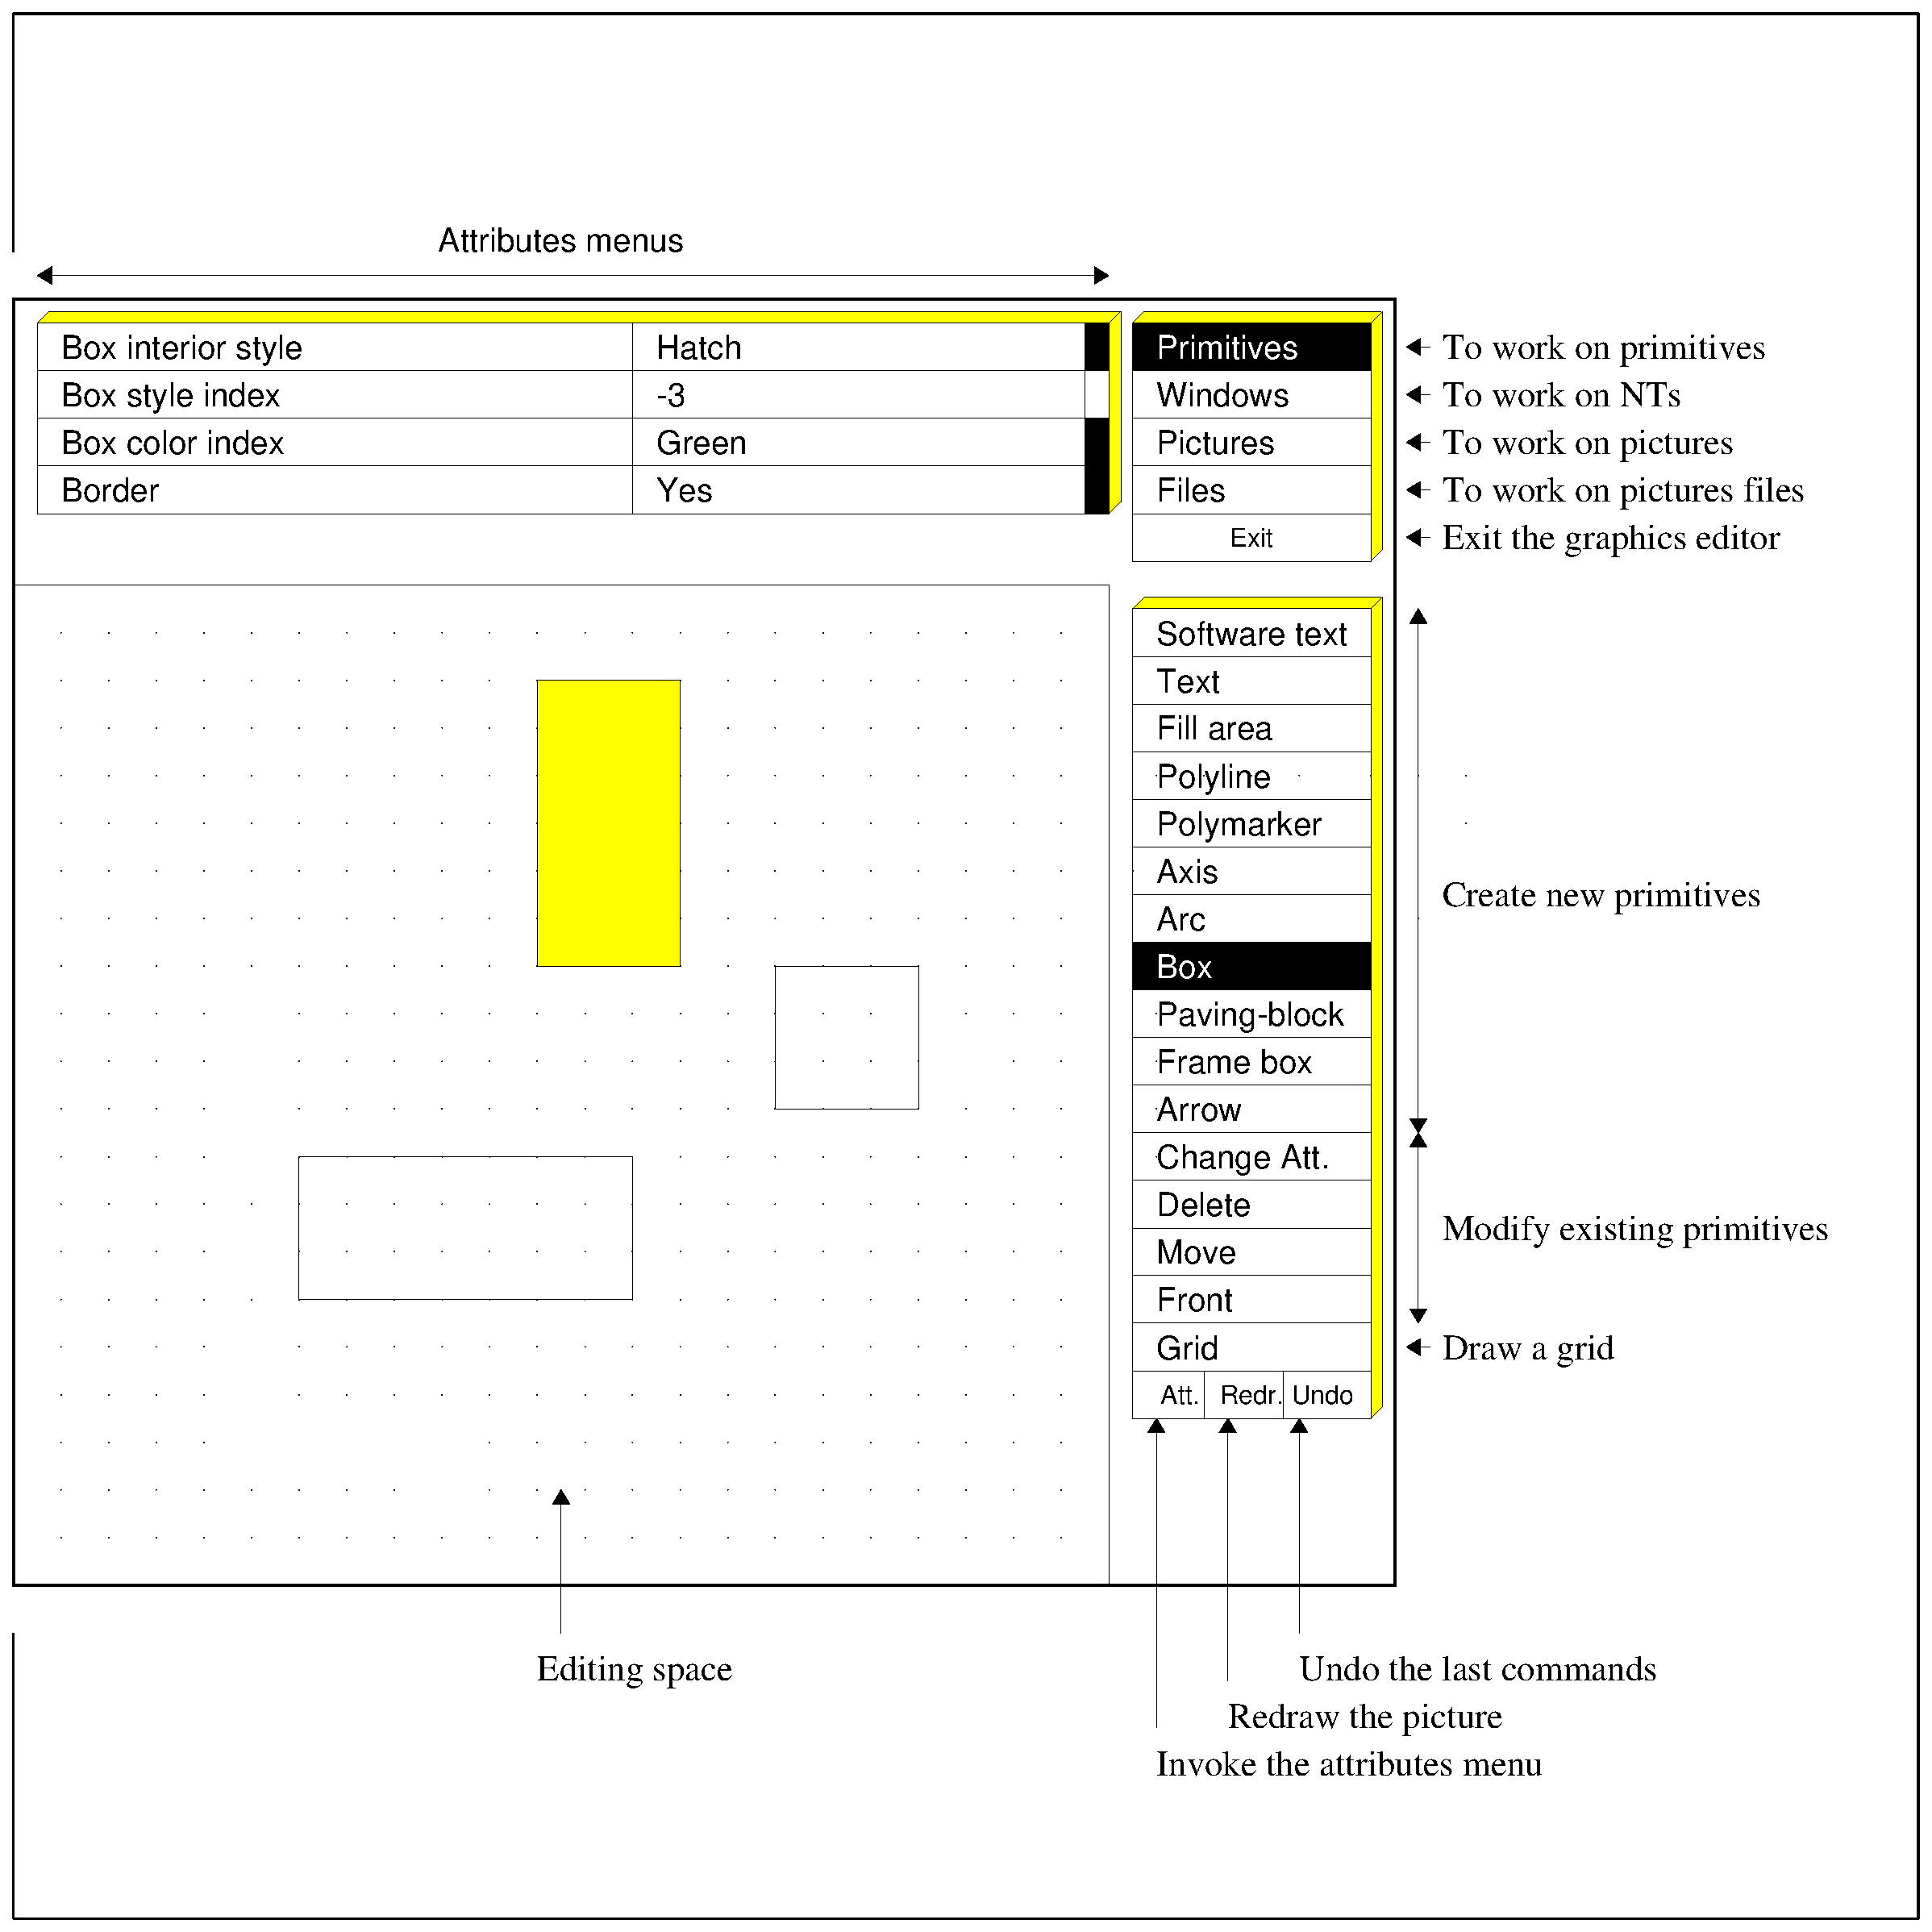
\epsfig{file=ged.eps,width=.9\textwidth}}
\end{center}
\caption{The graphics editor}
\label{fig-GED}
\end{Fighere}       
\end{minipage}
           % IZ routines
%%%%%%%%%%%%%%%%%%%%%%%%%%%%%%%%%%%%%%%%%%%%%%%%%%%%%%%%%%%%%%%%%%%%%%%%%%%%%%%%
%                                                                              %
%   HIGZ  User Guide -- LaTeX Source                                           %
%                                                                              %
%   Chapter: Picking                                                           %
%                                                                              %
%   Editor: Olivier Couet / CN-AS                                              %
%   Last Mod.:  9 July 1993 oc                                                 %
%                                                                              %
%%%%%%%%%%%%%%%%%%%%%%%%%%%%%%%%%%%%%%%%%%%%%%%%%%%%%%%%%%%%%%%%%%%%%%%%%%%%%%%%
\Filename{H1Structureandpicking}
\chapter{Structure and picking in the \HIGZ{} pictures}
\index{picking}
\Filename{H2TreestructureinHIGZpictures}
\section{Tree structure in \HIGZ{} pictures}
\index{picture!structure}
\Shubr{IGPID}{(LEVEL,NAME,PID,CHOPT)}
\Action
This routine allows to define {\it primitives identifiers} in the 
\HIGZ{} pictures. With this routine it is posible to define a tree 
structure inside \HIGZ{} pictures.
\Pdesc
\begin{DLtt}{12345678}
   \item[LEVEL] Level number
   \item[NAME] Primitives names
   \item[PID] Primitives identifier
   \item[CHOPT] Character options
   \begin{DLtt}{1234}
      \item[' '] the level becomes \Lit{LEVEL}
      \item['U'] one level Up
      \item['D'] one level Down
   \end{DLtt}
\end{DLtt}
\par
In the \HIGZ{} pictures, all the primitives stored sequentially {\bf after} a
{\it primitive identifier\/} are stamped with the \Rarg{LEVEL}, 
\Rarg{NAME} and \Rarg{PID}
defined by this {\it primitive identifier\/}. The level number allows 
to define a tree structure in the \HIGZ{} picture.

Some errors are prevented when using \Rind{IGPID}. One of these
errors is illustrated in the following:
if level 5 (for example) is requested when
the current level number is 1, then levels 2, 3 and 4
are not defined and  routine \Rind{IGPID} returns an error message.


\Filename{H2PickinginHIGZpictures}
\section{Picking in \HIGZ{} pictures}
\index{picture!picking}
\Shubr{IGPICK}{(NT*,*X*,*Y*,NBLEV*,NAME*,ID*,CHOPT)}
\Action
This routine allows to return the level number, the name and the
identifier of a picked primitive.
\Pdesc
\begin{DLtt}{1234567890}
   \item[NT] Normalization transformation
   \item[X, Y] Cursor position
   \item[NBLEV] Number of levels
   \item[NAME(NBLEV)] Names of the primitives
   \item[ID(NBLEV)] Identifiers of the primitives
   \item[CHOPT] Character options (Not used at present)
\end{DLtt}
In addition it is possible to get information via the common \QUEST.
\begin{DLtt}{12345678901}
   \item[IQUEST(60)] Adress of the picked primitive in the bank \Rarg{NT}. 
               If \Lit{IADR=0}, nothing has been picked.
   \item[IQUEST(61)] Primitive type
   \begin{DLtt}{123}
      \item[6] \Rind{IGHIST}
      \item[7] \Rind{IPM} with one point
      \item[8] \Rind{IPL} with two points
      \item[9] \Rind{IPL}
      \item[10] \Rind{IPM}
      \item[11] \Rind{IFA}
      \item[12] \Rind{ITX}
      \item[13] \Rind{IGBOX}
      \item[14] \Rind{IGFBOX}
      \item[15] \Rind{IGARC}
      \item[16] \Rind{IGAXIS}
      \item[17] \Rind{IGTEXT}
      \item[18] \Rind{IML}
      \item[20] \Rind{IGTABL}
   \end{DLtt}
\end{DLtt}
\par
By default the level 0 is the {\it Normalisation transformation} level.

\Filename{H2Selfstructuredprimitives}
\section{Self structured primitives}

It can be very inefficient to call \Rind{IGPID} and \Rind{IPM} with 1 point 
if  many hundreds of points have to be drawn. 
Routine \Rind{IPMID} solves this problem.

\Shubr{IPMID}{(N,X,Y,LEVEL,ID)}
\Action
This routine behave like \Rind{IPM} excepted that in the \HIGZ{}
picture each point is stamped with an identifier.
\Pdesc
\begin{DLtt}{12345678}
   \item[N] Number of points
   \item[X(N)] X coordinates
   \item[Y(N)] Y coordinates
   \item[LEVEL] Level number
   \item[ID(N)] Points identifier
\end{DLtt}

\begin{XMPt}{Example of structured picture (see result on figure \ref{PICK})}
      program pick
*
      common /pawc/ h(900000)
      character*8 chpid(15)
      dimension ipid(15)
*
      parameter (npts=20)
      dimension xz(86),yz(86)
      dimension x(npts),y(npts),id(npts)
      dimension xf1(3),yf1(3)
      dimension xf2(3),yf2(3)
      dimension xf3(3),yf3(3)
      dimension xf4(3),yf4(3)
      dimension xf5(3),yf5(3)
      data xf1/0.5,0.5,3.0/
      data yf1/0.5,4.0,0.5/
      data xf2/1.0,1.0,2.5/
      data yf2/1.0,3.5,1.0/
      data xf3/1.5,1.5,2.0/
      data yf3/1.5,3.0,1.5/
      data xf4/4.5,4.5,4.0/
      data yf4/1.0,4.0,2.0/
      data xf5/3.0,3.0,1.2/
      data yf5/4.0,4.5,1.1/
      data xz/
     +   0.6250,0.6875,0.9063,0.7500,0.7500,0.6875,0.6250,0.6875
     +  ,0.7500,0.8750,0.9688,1.0313,1.1563,1.2500,1.3125,1.5000
     +  ,1.6875,1.9375,2.0000,2.1250,2.1875,2.1875,2.2500,2.2500
     +  ,2.4375,2.4375,2.4688,2.5313,2.5313,2.5000,2.6250,2.6250
     +  ,2.7500,2.7188,2.7188,2.7188,2.9375,3.4375,3.7500,4.0625
     +  ,4.1250,4.0625,4.1250,4.1875,4.3125,4.3125,4.3125,4.3438
     +  ,4.3125,4.4375,4.5000,4.4375,4.4375,4.5625,4.5938,4.7188
     +  ,4.7813,4.7500,4.5313,4.5000,4.6250,4.6875,4.7188,4.7500
     +  ,4.8750,4.9625,4.9063,4.7500,4.6875,4.6563,4.3750,3.6875
     +  ,3.0625,2.8125,2.4375,2.0313,1.6563,1.4688,1.3438,1.3750
     +  ,1.4375,1.2500,1.1250,1.0000,0.8750,0.6250/
      data yz/
     +   4.8750,4.6563,4.3750,4.1250,3.8750,3.6250,3.4375,3.3125
     +  ,3.1875,3.1563,3.2188,3.3438,3.5000,3.5938,3.6875,3.5625
     +  ,3.3125,3.0938,2.8438,2.7000,2.2188,1.8750,1.2813,1.0625
     +  ,1.0625,1.8750,2.5000,2.4688,2.1875,1.9688,1.5000,1.2500
     +  ,1.2500,1.5313,2.0625,2.6250,2.5938,2.6563,2.7500,3.0000
     +  ,2.7188,2.1250,1.6563,1.4375,1.4688,1.6250,2.0313,2.3125
     +  ,2.6250,2.3125,2.0625,1.6250,1.5000,1.5000,1.6250,2.0313
     +  ,2.3125,2.5000,2.7500,2.9375,3.2500,3.6250,3.2500,2.8125
     +  ,2.6250,2.6875,3.0625,3.5625,3.8750,4.0625,4.1875,4.1250
     +  ,4.0313,4.0938,4.0625,4.2500,4.4875,4.5000,4.4688,4.6875
     +  ,4.8750,4.7188,4.5250,4.4688,4.7188,4.8750/
      data nz/86/
*
      call mzebra(-3)
      call mzpaw(900000,' ')
      call iginit(0)
      call igsse(6,1)
*
*          Create an HIGZ picture
*
      call izpict('PICT','M')
*
*          Define a new normalization transformation for each new object
*
      call iswn(10,0.,5.,0.,5.)
      call isvp(10,0.05,0.4,0.5,0.8)
      call iselnt(10)
      call igpid(1,'Zebra-axis',1,' ')
      call ipl(nz,xz,yz)
      call igaxis(.5,4.5,.5,.5,0.,1.,10,' ')
*
      call iswn(20,0.,7.,0.,7.)
      call isvp(20,0.5,0.8,0.5,0.8)
      call iselnt(20)
      call ismk(3)
      do j=1,7
         call ispmci(j)
         call igpid(1,'Ntuple',j,' ')
         do k=1,10
            do i=1,npts
               x(i)  = rndm(.01234)+float(j-1)
               y(i)  = 7.*rndm(.01234)
               id(i) = i 
            enddo
            call ipmid(npts,x,y,2,id)
         enddo
      enddo
*
      call iswn(30,0.,5.,0.,5.)
      call isvp(30,0.05,0.4,0.1,0.4)
      call iselnt(30)
      call isfais(1)
      call igpid(1,'Red',1,' ')
      call isfaci(2)
      call ifa(3,xf1,yf1)
      call igpid(2,'Green',2,' ')
      call isfaci(3)
      call ifa(3,xf2,yf2)
      call igpid(3,'Blue',3,' ')
      call isfaci(4)
      call ifa(3,xf3,yf3)
      call igpid(1,'Yellow',4,' ')
      call isfaci(5)
      call ifa(3,xf4,yf4)
      call igpid(1,'Magenta',5,' ')
      call isfaci(6)
      call ifa(3,xf5,yf5)
*
      call iswn(40,0.,5.,0.,5.)
      call isvp(40,0.5,0.85,0.1,0.4)
      call iselnt(40)
      call isfais(3)
      call isfasi(344)
      call isfaci(1)
      call igpid(1,'Zebra-fill',2,' ')
      call ifa(nz-1,xz,yz)
      call igpid(2,'Zebra-line',2,' ')
      call ipl(nz,xz,yz)
*
*              Picking loop
*
  10  call irqlc(1,1,ibut,nt,xloc,yloc)
      call igpick(nt,xloc,yloc,nblev,chpid,ipid,' ')
      print*,'==> Normalization Transformation: ',NT
      do i=1,nblev
         print*, '    Level: ',i,' Name: ',chpid(i),' ID: ',ipid(i)
      enddo
      if(ibut.ne.0)goto 10
*
      call igend
      end
\end{XMPt}

\begin{figure}[p]
\begin{center}
\mbox{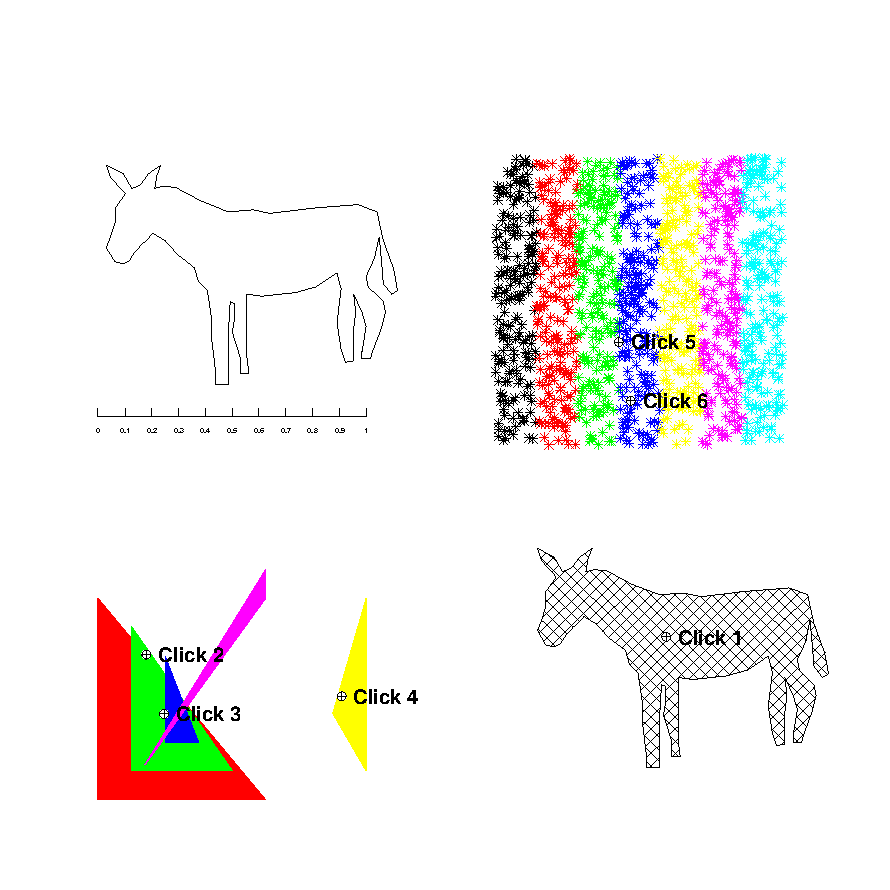
\epsfig{file=pick.eps,width=\the\textwidth}}
\end{center}
\caption{A structured picture}
\label{PICK}
\end{figure}

\newpage
The program {\tt pick} produce the following output if six ``click'' 
are done like on the figure \ref{PICK}.

\begin{XMPt}{Output produce by the program {\tt pick}}
 ==> Normalization Transformation:  40
     Level:  1 Name: Zebra-fi ID:  2
 ==> Normalization Transformation:  30
     Level:  1 Name: Red      ID:  1
     Level:  2 Name: Green    ID:  2
 ==> Normalization Transformation:  30
     Level:  1 Name: Red      ID:  1
     Level:  2 Name: Green    ID:  2
     Level:  3 Name: Blue     ID:  3
 ==> Normalization Transformation:  30
     Level:  1 Name: Yellow   ID:  4
 ==> Normalization Transformation:  20
     Level:  1 Name: Ntuple   ID:  4
     Level:  2 Name: POINT    ID:  4
 ==> Normalization Transformation:  20
     Level:  1 Name: Ntuple   ID:  4
     Level:  2 Name: POINT    ID:  4
\end{XMPt}

         % Picking
%%%%%%%%%%%%%%%%%%%%%%%%%%%%%%%%%%%%%%%%%%%%%%%%%%%%%%%%%%%%%%%%%%%%%%%%%%%%%%%%
%                                                                              %
%   HIGZ  User Guide -- LaTeX Source                                           %
%                                                                              %
%   Chapter: Interface routines with RZ                                        %
%                                                                              %
%   This document needs the following external EPS files:                      %
%     none                                                                     %
%                                                                              %
%   Editor: Michel Goossens / AS-MI                                            %
%   Last Mod.:  9 July 1993 oc                                                 %
%                                                                              %
%%%%%%%%%%%%%%%%%%%%%%%%%%%%%%%%%%%%%%%%%%%%%%%%%%%%%%%%%%%%%%%%%%%%%%%%%%%%%%%%
\Filename{H1Storingpictures}
\chapter{Storing pictures on ZEBRA/RZ direct access files}
\index{interface with RZ}

The routines described in this chapter allow the \HIGZ{} user to store pictures
on disk and retrieve them. The pictures created on disk by a given \HIGZ{} 
program can be used by other \HIGZ{} application programs. Facilities to list 
the contents of a RZ directory, to purge old cycles, create subdirectories, 
etc. are available in the \ZEBRA/RZ package.


\Filename{H2Interfaceroutines}
\section{Interface routines}
\index{interface routines}
\Shubr{IZFILE}{(LUN,CHDIR,CHOPT)}
\Action
This routine declares a pre-open direct acces file to be \ZEBRA/RZ file.
\Pdesc
\begin{DLtt}{1234567}
\item[LUN]   Logical unit number.
\item[CHDIR] {\tt CHARACTER} variable specifying the name of the top directory.
\item[CHOPT] {\tt CHARACTER} variable specifying the option(s) desired:
\begin{DLtt}{12345}
   \item['N'] Creates a {\bf N}ew RZ file with top directory name {\tt CHDIR}
   \item[' '] Open an existing RZ file with read only access.
   \item['U'] Open an existing RZ file in {\bf U}pdate mode.
   \item['A'] Pictures are {\bf A}utomatically saved on disk.
\end{DLtt}
\end{DLtt}
When option {\tt'A'} is given or when option \Sind{AURZ} is activated by 
\Rind{IGSET}, pictures are automatically saved into the RZ file. In this case,
there is only one picture in memory (the current picture). The last current 
picture is written on disk when \Rind{IGEND} is called.
 

\Shubr{IZOPEN}{(LUN,CHDIR,CFNAME,CHOPT,*LRECL*,ISTAT*)}
\Action
Open a HIGZ/RZ picture file. This routine open a direct access file and
call \Rind{IZFILE}. For more details see the description of the \ZEBRA{}
routine \Rind{RZOPEN} in the \ZEBRA{} manual.
\Pdesc
\begin{DLtt}{1234567}
\item[LUN]    Logical unit number.
\item[CHDIR]  {\tt CHARACTER} variable specifying the name of
              the top directory.
\item[CFNAME] File name.
\item[CHOPT]  {\tt CHARACTER} variable specifying the option(s) desired:
\begin{DLtt}{12345}
   \item['N'] Creates a {\bf N}ew RZ file with top directory name {\tt CHDIR}
   \item[' '] Open an existing RZ file with read only access.
   \item['U'] Open an existing RZ file in {\bf U}pdate mode.
   \item['A'] Pictures are {\bf A}utomatically saved on disk.
\end{DLtt}
\item[LRECL]  Integer variable specifying the record length of the file in 
              machine words. If a value of zero (0) is specified \Rind{IZOPEN}
              will attempt to obtain the correct record length from the file 
              itself. A value of zero must not be specified for new files.
\item[ISTAT]  Integer variable in which the status code is returned. 
\end{DLtt}
When option {\tt'A'} is given or when option \Sind{AURZ} is activated by 
\Rind{IGSET}, pictures are automatically saved into the RZ file. In this case,
there is only one picture in memory (the current picture). The last current 
picture is written on disk when \Rind{IGEND} is called.


\Shubr{IZIN}{(PNAME,ICYCLE)}
\Action
This routine reads a picture from an RZ data file and puts it in memory.
\Pdesc
\begin{DLtt}{1234567}
\item[PNAME] {\tt CHARACTER} variable specifying the name of picture to be read.
\item[ICYCLE] Cycle number of the picture to be read.
If {\tt ICYCLE} is greater than the highest existing cycle number on the RZ 
file, then the picture with the highest cycle number is read.
\end{DLtt}


\Shubr{IZOUT}{(PNAME,ICYCLE*)}
\Action
This routine writes on an RZ data file a memory resident picture.
\Pdesc
\begin{DLtt}{12345678}
\item[PNAME] {\tt CHARACTER} variable specifying the name of picture to be
             written.
\item[ICYCLE*] Cycle number of the picture written. If a picture with name 
               {\tt PNAME} does not already exist on the output file, then a 
               value for {\tt ICYCLE} of {\tt 1} is returned, otherwise a value
               one higher than the (previous) highest cycle number on the file.
\end{DLtt}


\Shubr{IZSCR}{(PNAME,ICYCLE)}
\Action
This routine deletes (scratches) a picture from an RZ data file.
\Pdesc
\begin{DLtt}{1234567}
\item[PNAME] {\tt CHARACTER} variable specifying the name of
picture to be deleted.
\item[ICYCLE] Cycle number of the picture to be deleted.
\end{DLtt}
           % ZEBRA RZ routine interface
%%%%%%%%%%%%%%%%%%%%%%%%%%%%%%%%%%%%%%%%%%%%%%%%%%%%%%%%%%%%%%%%%%%%%%%%%%%%%%%%
%                                                                              %
%   HIGZ  User Guide -- LaTeX Source                                           %
%                                                                              %
%   Chapter: The miscellaneous functions                                       %
%                                                                              %
%   Editor: Olivier Couet / CN-AS                                              %
%   Last Mod.: 9 July 1993 oc                                                  %
%                                                                              %
%%%%%%%%%%%%%%%%%%%%%%%%%%%%%%%%%%%%%%%%%%%%%%%%%%%%%%%%%%%%%%%%%%%%%%%%%%%%%%%%
\Filename{H1miscellaneousfunctions}
\chapter{miscellaneous functions}
\index{miscellaneous functions}

User routines, whose functionality is often needed (e.g. displaying a message),
but which cannot be classified easily in any of the previous chapters will be
described in this chapter.

\Filename{H2Displayamessageonthescreen}
\section{Display a message on the screen}
\index{message on the screen}
\Shubr{IGMESS}{(N,CHMESS,CHTIT,CHOPT)}
\Action
This routine allows to display a message. The \X11{} version of \HIGZ{} displays
the message in a separated window.
\Pdesc
\begin{DLtt}{1234567}
\item[N] Number of lines in the message.
\item[CHMESS(N)] Message to be displayed.
\item[CHTIT] Window title.
\item[CHOPT] Options.
\begin{DLtt}{12345}
\item['P'] Print the array \Rarg{CHMESS} and open the message window
if necessary.
\item['C'] Close the message window.
\item['T'] Print the array \Rarg{CHMESS} on standard output.
\item['D'] Delete the message window.
\end{DLtt}
\end{DLtt}
\Filename{H2Displayacolourmap}
\section{Display a colour map}
\index{display!colour map}
\Shubr{IGCOLM}{(X1,X2,Y1,Y2,IC1,IC2,ZMIN,ZMAX,CHOPT)}
\Action
This routine allows to display a colour map on the screen.
\Pdesc
\begin{DLtt}{1234567}
\item[X1] X coordinate of 1st corner of the rectangle in \WC.
\item[X2] X coordinate of 2nd corner of the rectangle in \WC.
\item[Y1] Y coordinate of 1st corner of the rectangle in \WC.
\item[Y2] Y coordinate of 2nd corner of the rectangle in \WC.
\item[IC1] First colour index.
\item[IC2] Last colour index
\item[ZMIN] Minimum Z value.
\item[ZMAX] Maximum Z value.
\item[CHOPT] Options.
\begin{DLtt}{12345}
\item['C'] Draw the levels with \Em{C}olours.
\item['B'] Draw the levels with \Em{B}oxes.
\item['A'] Draw the \Em{A}xis.
\item['H'] Draw the map \Em{H}orizontally (default is vertically).
\end{DLtt}
\end{DLtt}

\newpage

\Filename{H2ConversionbetweenColoursystems}
\section{Conversion between Colour systems}
\index{colour!systems!HLS}
\index{colour!systems!RGB}

\subsection{RGB to HLS}
\Shubr{IGRTOH}{(CR,CB,CG,CH*,CL*,CS*)}
\Action
This routine convert a RGB colour into an HLS colour.
\Pdesc
\begin{DLtt}{1234567}
\item[CR] Red value \Lit{0.\(\leq\)CR\(\leq\)1.}
\item[CG] Green value \Lit{0.\(\leq\)CG\(\leq\)1.}
\item[CB] Blue value \Lit{0.\(\leq\)CB\(\leq\)1.}
\item[CH] Hue value \Lit{0.\(\leq\)CH\(\leq\)360.}
\item[CL] Light value \Lit{0.\(\leq\)CL\(\leq\)1.}
\item[CS] Saturation value \Lit{0.\(\leq\)CS\(\leq\)1.}
\end{DLtt}

\subsection{HLS to RGB}
\Shubr{IGHTOR}{(CH,CL,CS,CR*,CB*,CG*)}
\Action
This routine convert a HLS colour into an RGB colour.
\Pdesc
\begin{DLtt}{1234567}
\item[CH] Hue value \Lit{0.\(\leq\)CH\(\leq\)360.}
\item[CL] Light value \Lit{0.\(\leq\)CL\(\leq\)1.}
\item[CS] Saturation value \Lit{0.\(\leq\)CS\(\leq\)1.}
\item[CR] Red value \Lit{0.\(\leq\)CR\(\leq\)1.}
\item[CG] Green value \Lit{0.\(\leq\)CG\(\leq\)1.}
\item[CB] Blue value \Lit{0.\(\leq\)CB\(\leq\)1.}
\end{DLtt}

\newpage
 
\Filename{H2Conversionbetweencharacterstringandnumbers}
\section{Conversion between character string and numbers}
\index{character!conversion to number}
\index{number!conversion to character}

Often it is necessary to convert a \FORTRAN{} character string into
a number (integer or real) or vice versa. For example, routine \Rind{IGMENU}
returns some parameters as character strings and it is often necessary to convert
these into numbers. 
Also, to print graphically the result of a computation with
\Rind{ITX} it is necessary to convert a number into a character string. 
The routines described in this paragraph allow these kinds of conversions.

\subsection{Character to integer}
\Shubr{IZCTOI}{(CHVAL,IVAL*)}
\Action
Converts the character string {\tt CHVAL} into the integer {\tt IVAL}.
\Pdesc
\begin{DLtt}{1234567}
\item[CHVAL] Character string.
\item[IVAL] Integer.
\end{DLtt}

\subsection{Character to real}
\Shubr{IZCTOR}{(CHVAL,RVAL*)}
\Action
Converts the character string {\tt CHVAL} into the real {\tt RVAL}.
\Pdesc
\begin{DLtt}{1234567}
\item[CHVAL] Character string.
\item[RVAL] Real.
\end{DLtt}
\subsection{Integer to character}
\Shubr{IZITOC}{(IVAL,CHVAL*)}
\Action
Converts the integer {\tt IVAL} into character string {\tt CHVAL}.
\Pdesc
\begin{DLtt}{1234567}
\item[IVAL] Integer.
\item[CHVAL] Character string.
\end{DLtt}
\subsection{Real to character}
\Shubr{IZRTOC}{(RVAL,CHVAL*)}
\Action
Converts the real {\tt RVAL} into character string {\tt CHVAL}.
\Pdesc
\begin{DLtt}{1234567}
\item[RVAL] Real.
\item[CHVAL] Character string.
\end{DLtt}
         % Graphics input
%%%%%%%%%%%%%%%%%%%%%%%%%%%%%%%%%%%%%%%%%%%%%%%%%%%%%%%%%%%%%%%%%%%%%%%%%%%%%%%%
%                                                                              %
%   HIGZ  User Guide -- LaTeX Source                                           %
%                                                                              %
%   Chapter: HIGZ examples                                                     %
%                                                                              %
%   Editor: Olivier Couet / CN-AS                                              %
%   Last Mod.:  9 July oc                                                      %
%                                                                              %
%%%%%%%%%%%%%%%%%%%%%%%%%%%%%%%%%%%%%%%%%%%%%%%%%%%%%%%%%%%%%%%%%%%%%%%%%%%%%%%%
\Filename{H1ExamplesofHIGZoutput}
\chapter{Examples of \HIGZ{} output}

The graphical results of the examples below are reproduced directly 
from the \PS{} output of and introduced into this manual.

\begin{XMPt}{\HIGZ{} test program}
      PROGRAM HIGZEX
*.==========>
*.
*.           HIGZ TEST PROGRAM
*.
*..=========>
      COMMON/PAWC/H(20000)
      LOGICAL INTRAC
      CHARACTER*80 STR
      CHARACTER*(*) HZFILE
+SELF,IF=IBM,IF=-PSCRIPT.
      PARAMETER (HZFILE='/HIGZ METAFILE')
+SELF,IF=IBM,IF=PSCRIPT.
      PARAMETER (HZFILE='/HIGZ PS')
+SELF,IF=-IBM,IF=-PSCRIPT.
      PARAMETER (HZFILE='higz.metafile')
+SELF,IF=-IBM,IF=PSCRIPT.
      PARAMETER (HZFILE='higz.ps')
+SELF.

*.___________________________________________
*
+SELF,IF=IBM.
      CALL ERRSET(151,999,-1)
+SELF,IF=IBM,IF=X11.
      CALL INITC()
+SELF.
      OPEN(10,FILE=HZFILE,FORM='FORMATTED',STATUS='UNKNOWN')
      CALL MZEBRA(-3)
      CALL MZPAW(20000,' ')
      CALL IGINIT(0)
      IF(.NOT.INTRAC(DUMMY))THEN
         INTER=0
         KWTYPE=0
      ELSE
         CALL IGWKTY(KWTYPE)
         INTER=1
      ENDIF
      CALL IGSSE(6,KWTYPE)
      IF(INTER.EQ.0)GOTO 10
      CALL HIEX1
      CALL IRQST(1,1,ISTAT,NCH,STR)
*
*          Switch to alpha mode. Note that IGSSE has preset the
*          workstation identifier to 1
*
      CALL IGSA (1)
*
      PRINT *, ' Example 1 completed'
      CALL HIEX2
      CALL IRQST(1,1,ISTAT,NCH,STR)
      CALL IGSA (1)
      PRINT *, ' Example 2 completed'
*
      CALL HIEX3
      CALL IRQST(1,1,ISTAT,NCH,STR)
      CALL IGSA (1)
      PRINT *, ' Example 3 completed'
*
      CALL HIEX4
      CALL IRQST(1,1,ISTAT,NCH,STR)
      CALL IGSA (1)
      PRINT *, ' Example 4 completed'
*
  10  CALL HIEX5
      IF(INTER.EQ.0)GOTO 20
      CALL IGSA (1)
      PRINT *, ' Example 5 completed'
*
*          Replay some pictures from the HIGZ metafile
*
      CALL HIEX6
      CALL IGSA (1)
      PRINT *, ' Example 6 completed'
*
  20  CALL IGEND
      END
\end{XMPt}

\newpage
\begin{XMPt}{Example of basic HIGZ. Polylines and fill areas}
\label{HIEX1}
      SUBROUTINE HIEX1
*
      COMMON /QUEST/ RQUEST(100)
      DIMENSION XZ(86),YZ(86)
      DATA XZ/
     +   0.6250,0.6875,0.9063,0.7500,0.7500,0.6875,0.6250,0.6875
     +  ,0.7500,0.8750,0.9688,1.0313,1.1563,1.2500,1.3125,1.5000
     +  ,1.6875,1.9375,2.0000,2.1250,2.1875,2.1875,2.2500,2.2500
     +  ,2.4375,2.4375,2.4688,2.5313,2.5313,2.5000,2.6250,2.6250
     +  ,2.7500,2.7188,2.7188,2.7188,2.9375,3.4375,3.7500,4.0625
     +  ,4.1250,4.0625,4.1250,4.1875,4.3125,4.3125,4.3125,4.3438
     +  ,4.3125,4.4375,4.5000,4.4375,4.4375,4.5625,4.5938,4.7188
     +  ,4.7813,4.7500,4.5313,4.5000,4.6250,4.6875,4.7188,4.7500
     +  ,4.8750,4.9625,4.9063,4.7500,4.6875,4.6563,4.3750,3.6875
     +  ,3.0625,2.8125,2.4375,2.0313,1.6563,1.4688,1.3438,1.3750
     +  ,1.4375,1.2500,1.1250,1.0000,0.8750,0.6250/
      DATA YZ/
     +   4.8750,4.6563,4.3750,4.1250,3.8750,3.6250,3.4375,3.3125
     +  ,3.1875,3.1563,3.2188,3.3438,3.5000,3.5938,3.6875,3.5625
     +  ,3.3125,3.0938,2.8438,2.7000,2.2188,1.8750,1.2813,1.0625
     +  ,1.0625,1.8750,2.5000,2.4688,2.1875,1.9688,1.5000,1.2500
     +  ,1.2500,1.5313,2.0625,2.6250,2.5938,2.6563,2.7500,3.0000
     +  ,2.7188,2.1250,1.6563,1.4375,1.4688,1.6250,2.0313,2.3125
     +  ,2.6250,2.3125,2.0625,1.6250,1.5000,1.5000,1.6250,2.0313
     +  ,2.3125,2.5000,2.7500,2.9375,3.2500,3.6250,3.2500,2.8125
     +  ,2.6250,2.6875,3.0625,3.5625,3.8750,4.0625,4.1875,4.1250
     +  ,4.0313,4.0938,4.0625,4.2500,4.4875,4.5000,4.4688,4.6875
     +  ,4.8750,4.7188,4.5250,4.4688,4.7188,4.8750/
      DATA NZ/86/
*
*          Define the size of the Picture in cm
*
      CALL ICLRWK(0,1)
      CALL IGRNG(14.5,14.5)
      R  = RQUEST(11)
      XL = RQUEST(12)
      YB = RQUEST(13)
      CALL IGBOX(0.,14.5,0.,14.5)
      CALL IGTEXT(7.25,13.5,'HIGZ example 1',0.6,0.,'C')
*
*          Define a new Normalization transformation for each new object
*          The viewports are set in the centimeter space defined by IGRNG
*
      CALL ISWN(10,0.,5.,0.,5.)
      CALL ISVP(10,0.5*R+XL,6.5*r+XL,6.5*R+YB,11.5*r+YB)
      CALL ISELNT(10)
      CALL IPL(NZ,XZ,YZ)
*
      CALL ISWN(20,0.,5.,0.,5.)
      CALL ISVP(20,7.5*R+XL,14.*r+XL,6.5*R+YB,11.5*r+YB)
      CALL ISELNT(20)
      CALL ISMK(29)
      CALL IPM(NZ-1,XZ,YZ)
      CALL IPL(NZ  ,XZ,YZ)
*
      CALL ISWN(30,0.,5.,0.,5.)
      CALL ISVP(30,0.5*R+XL,6.5*r+XL,0.5*R+YB,5.5*r+YB)
      CALL ISELNT(30)
      CALL ISFAIS(3)
      CALL ISFASI(256)
      CALL IFA(NZ-1,XZ,YZ)
*
      CALL ISWN(40,0.,5.,0.,5.)
      CALL ISVP(40,7.5*R+XL,14.*r+XL,0.5*R+YB,5.5*r+YB)
      CALL ISELNT(40)
      CALL ISFASI(290)
      CALL IFA(NZ-1,XZ,YZ)
      CALL ISFAIS(0)
      CALL IFA(NZ-1,XZ,YZ)
*
      END
\end{XMPt}
\newpage

\begin{minipage}{\textwidth}
\begin{Fighere}
\begin{center}\mbox{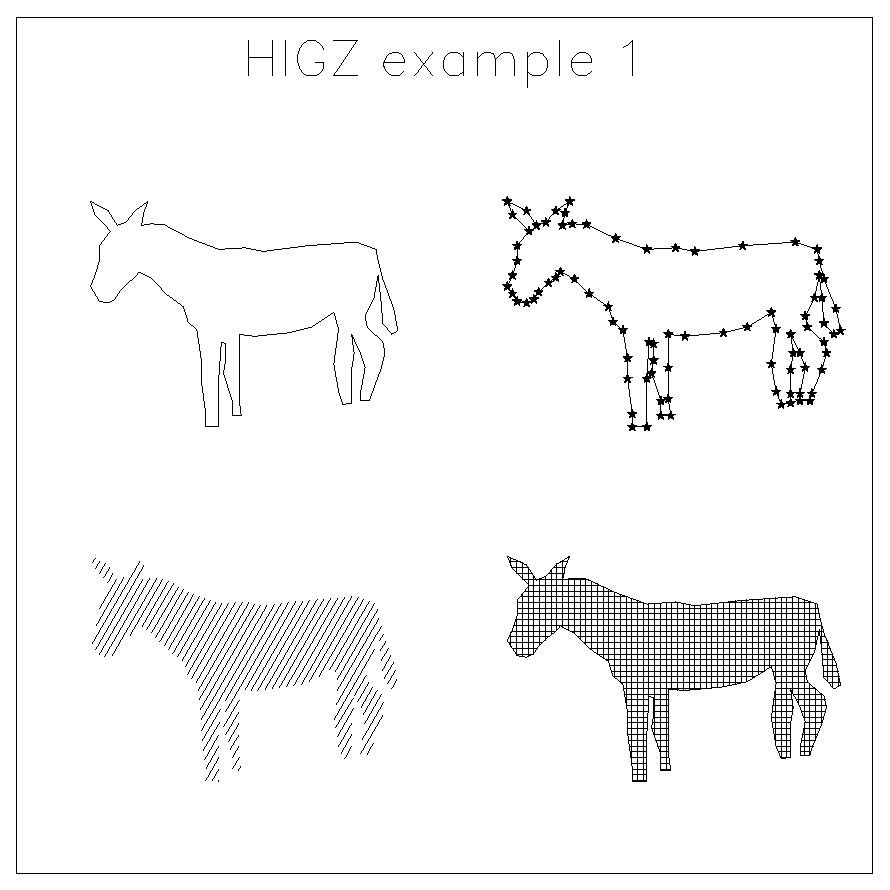
\epsfig{file=higz1.eps}}\end{center}
\caption{Result of first \protect\HIGZ{} example}
\end{Fighere}
\end{minipage}

\newpage

\begin{XMPt}{Example to plot the table of \HIGZ{} software characters}
      SUBROUTINE HIEX2
*
      CHARACTER*6 KD1,KD2
      CHARACTER*45 KDG
      CHARACTER*3 KTEXT
      CHARACTER*1 CHOPT
      DIMENSION XPOS(6),X(5),Y(5)
      DATA KD1/' < < <'/
      DATA KD2/'  [[""'/
      DATA KDG/'ABCDEFGHIJKLMNOPQRSTUVWXYZ0123456789.,+-*/=()'/
      DATA XLONG,YTOP/16.,24./
      DATA SIZE,ANGLE/0.3,0./
*
      CALL IGRNG(20.,24.)
      CALL ICLRWK(0,1)
*
      XW = XLONG/12.
      DO 10 I = 1,6
         XPOS(I) = (2*I-1)*XW + 2.5
  10  CONTINUE
*
*              Draw the frame
*
      YLONG  = 46*1.5*SIZE + 5*1.5*SIZE
      X(1)   = XPOS(1) - XW
      X(2)   = XPOS(6) + XW
      X(3)   = X(2)
      X(4)   = X(1)
      X(5)   = X(1)
      Y(1)   = YTOP
      Y(2)   = Y(1)
      Y(3)   = Y(1) - YLONG
      Y(4)   = Y(3)
      Y(5)   = Y(1)
      CALL IPL(5,X,Y)
      DO 20 I = 1,5
         X(1)   = XPOS(I) + XW
         X(2)   = X(1)
         Y(1)   = YTOP
         Y(2)   = Y(1) - YLONG
         CALL IPL(2,X,Y)
  20  CONTINUE
      X(1)   = XPOS(1) - XW
      X(2)   = XPOS(6) + XW
      Y(1)   = YTOP - 5.*SIZE
      Y(2)   = Y(1)
      CALL IPL(2,X,Y)
*
*             Draw box titles
*
      Y1     = YTOP - 2.*SIZE
      Y2     = Y1 - 2.*SIZE
      CHOPT='C'
      CALL IGTEXT(XPOS(1),Y1,'Upper'  ,SIZE,ANGLE,CHOPT)
      CALL IGTEXT(XPOS(1),Y2,'Roman'  ,SIZE,ANGLE,CHOPT)
      CALL IGTEXT(XPOS(2),Y1,'Lower'  ,SIZE,ANGLE,CHOPT)
      CALL IGTEXT(XPOS(2),Y2,'Roman'  ,SIZE,ANGLE,CHOPT)
      CALL IGTEXT(XPOS(3),Y1,'Upper'  ,SIZE,ANGLE,CHOPT)
      CALL IGTEXT(XPOS(3),Y2,'Greek'  ,SIZE,ANGLE,CHOPT)
      CALL IGTEXT(XPOS(4),Y1,'L<OWER' ,SIZE,ANGLE,CHOPT)
      CALL IGTEXT(XPOS(4),Y2,'G<REEK' ,SIZE,ANGLE,CHOPT)
      CALL IGTEXT(XPOS(5),Y1,'U<PPER' ,SIZE,ANGLE,CHOPT)
      CALL IGTEXT(XPOS(5),Y2,'Special',SIZE,ANGLE,CHOPT)
      CALL IGTEXT(XPOS(6),Y1,'Lower'  ,SIZE,ANGLE,CHOPT)
      CALL IGTEXT(XPOS(6),Y2,'Special',SIZE,ANGLE,CHOPT)
*
      YP = YTOP - 6.*SIZE
      DO 40 I = 1,45
         YP = YP - 1.5*SIZE
         DO 30 J = 1,6
            KTEXT=KD1(J:J)//KD2(J:J)//KDG(I:I)
            CALL IGTEXT(XPOS(J),YP,KTEXT,SIZE,ANGLE,CHOPT)
  30     CONTINUE
  40  CONTINUE
*
      END
\end{XMPt}

\begin{figure}[p]
\begin{center}\mbox{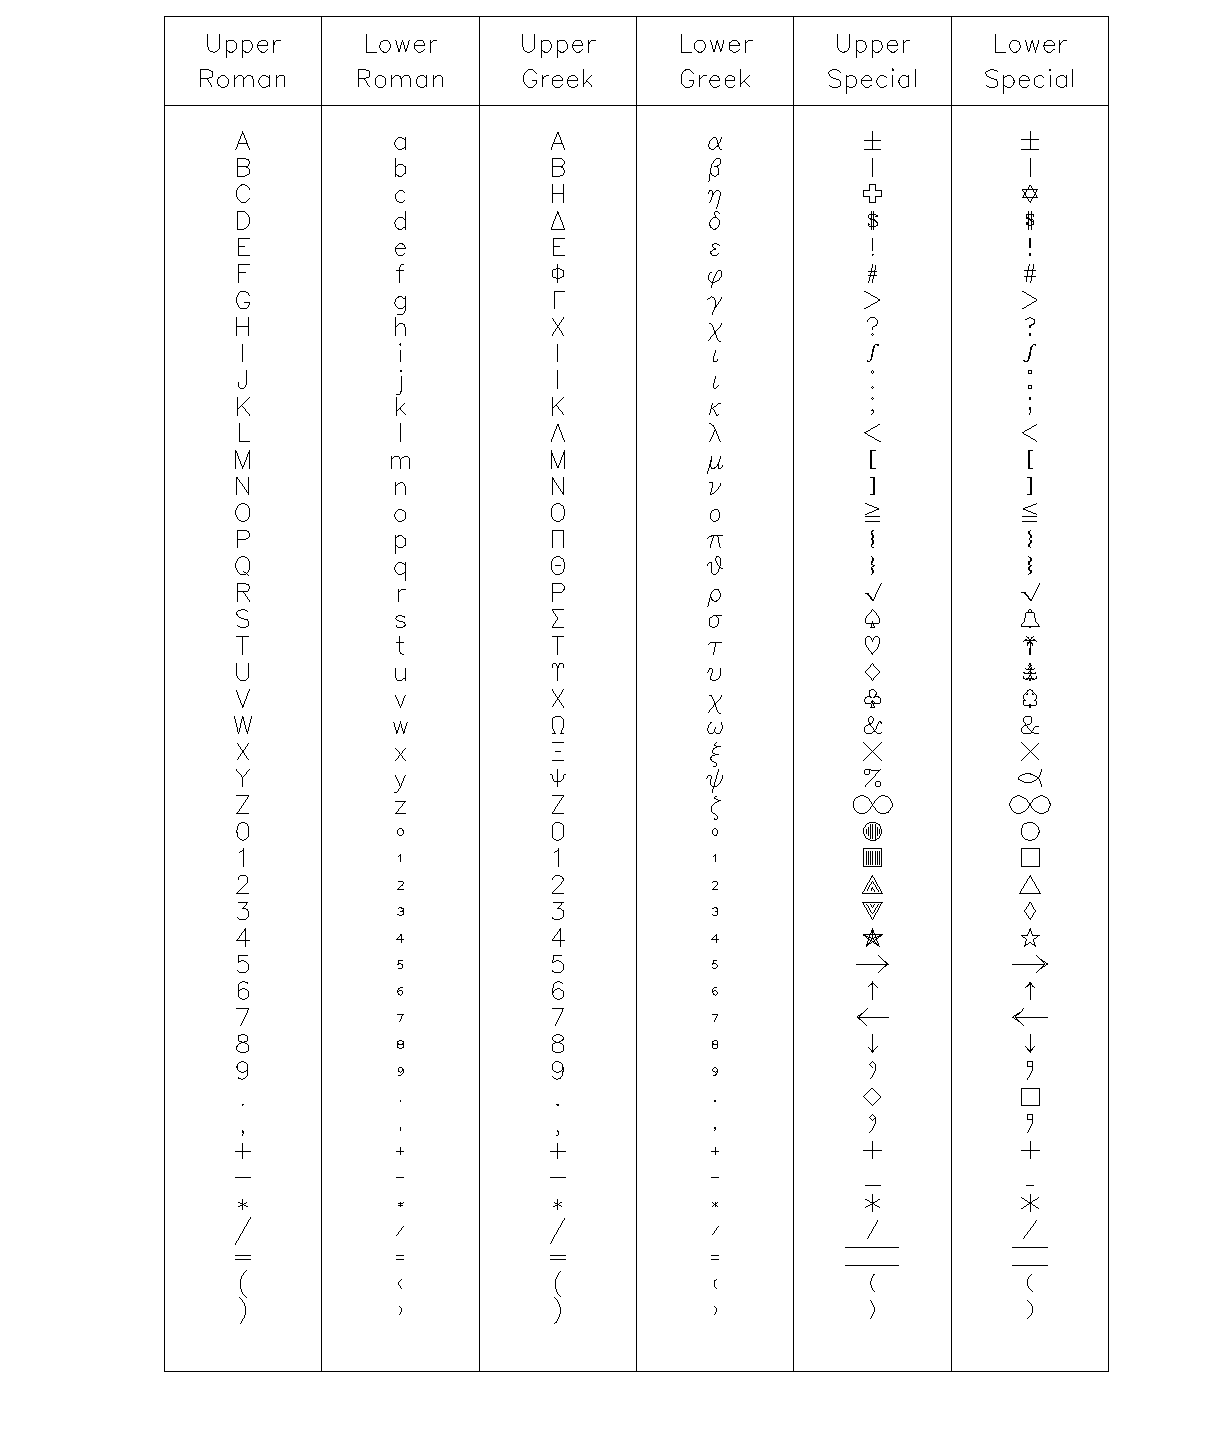
\epsfig{file=higz2.eps,width=\textwidth}}\end{center}
\caption{Result of plotting \protect\HIGZ{} software characters}
\end{figure}
\clearpage

\begin{XMPt}{Advanced example to draw text (based on a PAW macro from W.Walk)}
      SUBROUTINE HIEX3
*
      DIMENSION X(3),Y(3)
*
      CALL IGRNG(14.6,18.)
      CALL ICLRWK(0,1)
      CALL IGBOX(0.,14.6,0.,18.)
      CALL IGSET('PASS',10.)
      CALL IGSET('CSHI',0.005)
      CALL ISFAIS(1)
      CALL ISTXCI(1)
      CALL ISTXFP(-104,2)
      CALL ISCHH(0.6)
      CALL ISTXAL(2,0)
      CALL ITX(7.3,17.,'Exclusive Toponium Decays')
      CALL ISTXFP(0,2)
      CALL ISFACI(1)
      CALL IGBOX(5.,7.,15.,14.9)
      CALL IGBOX(5.,7.,3.,2.9)
      CALL IGBOX(3.,5.,14.,13.9)
      CALL IGBOX(3.,5.,2.,1.9)
      CALL IGBOX(10.,12.,13.,12.9)
      CALL IGBOX(10.,12.,12.,11.9)
      CALL IGBOX(10.,12.,11.,10.9)
      CALL IGBOX(6.,8.,12.4,12.3)
      CALL ISPLCI(3)
      X(1)=6.
      X(2)=11.
      X(3)=6.
      Y(1)=15.
      Y(2)=13.
      Y(3)=3.
      CALL IPL(3,X,Y)
      Y(2)=12.
      CALL IPL(3,X,Y)
      Y(2)=11.
      CALL IPL(3,X,Y)
      CALL ISPLCI(2)
      X(2)=4.
      Y(2)=14.
      CALL IPL(3,X,Y)
      Y(2)=2.
      CALL IPL(3,X,Y)
      CALL ISPLCI(4)
      X(2)=X(3)
      Y(2)=1.5
      CALL IPL(2,X(2),Y(2))
      X(1)=X(2)-0.2
      X(3)=X(2)+0.2
      Y(1)=Y(2)+0.3
      Y(3)=Y(1)
      CALL IPL(3,X,Y)
      CALL ISTXCI(4)
      CALL IGTEXT(6.,0.5,'e^+!e^-! or [m]^+![m]^-!',0.5,0.,'C')
      CALL IGTEXT(6.,15.2,'2^3!S?1--!',0.5,0.,'C')
      CALL IGTEXT(6.,3.2,'1^3!S?1--!',0.5,0.,'C')
      CALL IGTEXT(11.,13.2,'1^3!P?2++!',0.5,0.,'C')
      CALL IGTEXT(11.,12.2,'1^3!P?1++!',0.5,0.,'C')
      CALL IGTEXT(11.,11.2,'1^3!P?0++!',0.5,0.,'C')
      CALL IGTEXT(7.,12.6,'1^1!P?1+-!',0.5,0.,'C')
      CALL IGTEXT(4.,14.2,'2^1!S?0-+!',0.5,0.,'C')
      CALL IGTEXT(4., 2.2,'1^1!S?0-+!',0.5,0.,'C')
      CALL ISTXCI(6)
      CALL IGTEXT(4.5,15.,'[Q]?2S!',0.5,0.,'R')
      CALL IGTEXT(7.5,2.75,'[Q]?1S! (80 GeV)',0.5,0.,'L')
      CALL IGTEXT(2.5,13.75,'[c]?t!&^,!',0.5,0.,'R')
      CALL IGTEXT(2.5,1.75,'[c]?t!',0.5,0.,'R')
      CALL IGTEXT(12.5,13.,'[h]^2!&?t!',0.5,0.,'L')
      CALL IGTEXT(12.5,12.,'[h]^1!&?t!',0.5,0.,'L')
      CALL IGTEXT(12.5,11.,'[h]^0!&?t!',0.5,0.,'L')
      CALL ISTXCI(3)
      CALL IGTEXT(1.,9.,'E1',0.5,0.,'C')
      CALL ISTXCI(2)
      CALL IGTEXT(3.,9.,'M1',0.5,0.,'C')
      CALL ISTXCI(3)
      CALL IGTEXT(8.8,14.8,'100 MeV',0.4,0.,'L')
      CALL IGTEXT(8.5,6.,'800 MeV',0.4,0.,'L')
      CALL ISTXCI(6)
      CALL IGTEXT(9.4,14.2,'BR 2"Y',0.3,0.,'L')
      CALL IGTEXT(8.9,5.4,'BR 30"Y',0.3,0.,'L')
      CALL IGSET('*',0.)
*
      END
\end{XMPt}

\begin{figure}[p]
\begin{center}\mbox{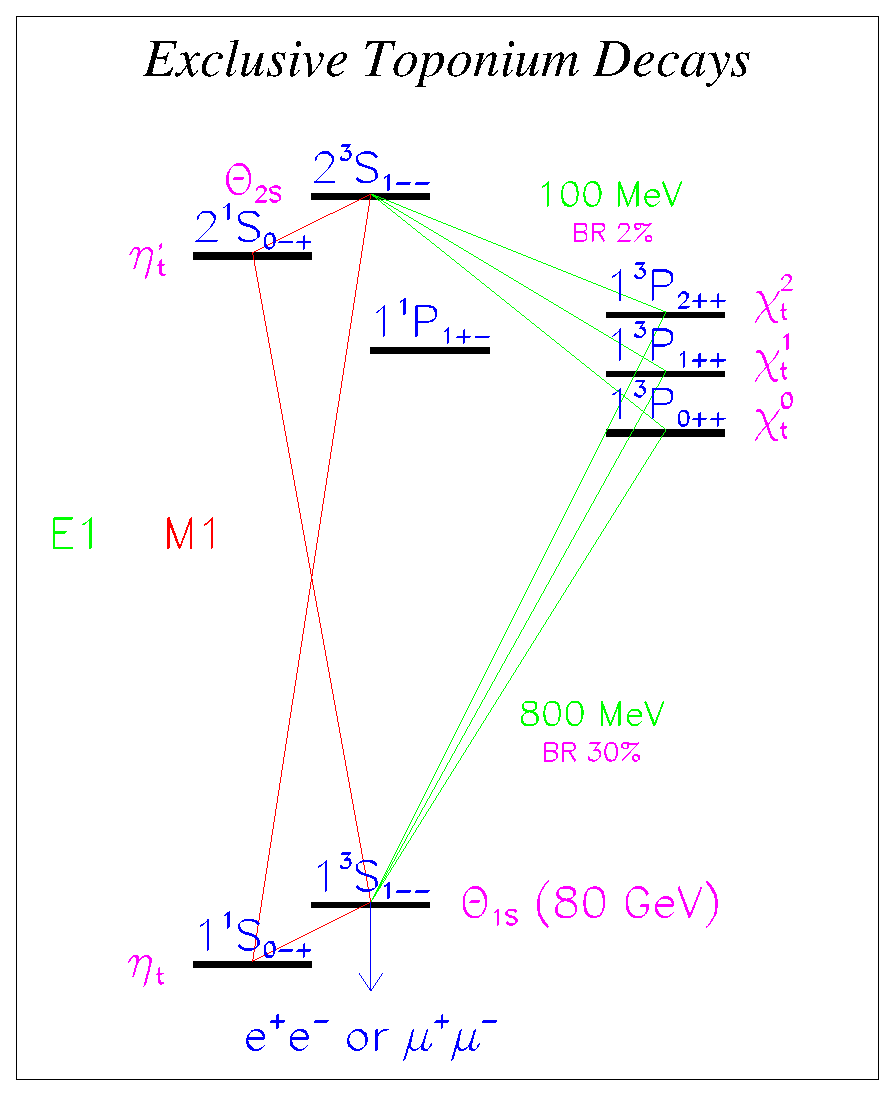
\epsfig{file=higz3.eps}}\end{center}
\caption{Result of \protect\HIGZ{} example 3 (toponium decay scheme)}
\end{figure}
\clearpage

\begin{XMPt}{Examples of graphs and histograms}
\label{HIEX4}
      SUBROUTINE HIEX4
*
      COMMON /QUEST/ RQUEST(100)
      DIMENSION X(10),Y(10),V(10)
      DATA Y/2.,3.,5.,4.,7.,10.,11.,9.,10.,4./
      DATA X/0.,16.,8*0./
      DATA V/-1.5,1.,2.,4.,4.5,6.,9.,10.,14.,17./
*
      CALL IGRNG(15.,18.)
      R  = RQUEST(11)
      XL = RQUEST(12)
      YB = RQUEST(13)
      CALL ICLRWK(0,1)
      CALL ISTXFP(-13,1)
*
      CALL ISWN(10,0.,18.,-1.,12.)
      CALL ISVP(10,8.*R+XL,14.*R+XL,11.*R+YB,17.*R+YB)
      CALL ISELNT(10)
      CALL ISMK(29)
      CALL IGHIST(10,X,Y,'AHCP')
*
      CALL ISWN(20,0.,18.,0.,12.)
      CALL ISVP(20,R+XL,7.*R+XL,11.*R+YB,17.*R+YB)
      CALL ISELNT(20)
      CALL IGHIST(10,X,Y,'AB')
*
      CALL ISWN(30,-4.,19.,-1.,13.)
      CALL ISVP(30,R+XL,14.*R+XL,R+YB,10.*R+YB)
      CALL ISELNT(30)
      CALL IGAXIS(-3.,19.,1.,1.,-3.,19.,20510,' ')
      CALL IGSET('LASI',0.5)
      CALL IGAXIS(-3.,-3.,1.,12.,1.,12.,510,'H')
      CALL ISMK(21)
      CALL IGRAPH(10,V,Y,'LP')
      CALL ISLN(2)
      CALL IGRAPH(10,V,Y,'C')
      CALL IGSET('*',0.)
*
      END
\end{XMPt}

\begin{figure}[p]
\begin{center}\mbox{\epsfig{file=higz4.eps}}\end{center}
\caption{Result of \protect\HIGZ{} example 4 (graphs and histograms)}
\end{figure}
\clearpage

\begin{XMPt}{Example using \HIGZ{} and \PS{} metafiles}
      SUBROUTINE HIEX5
*
*          Open HIGZ metafile
*          and repeat previous examples
*
      PRINT *,' Writing higz metafile'
      CALL IGZSET('Z')
      CALL IZOPEN(1,'Pictures','higz.rz','AN',1024,ISTAT)
      CALL IZPICT('ZEBRA','M')
      CALL HIEX1
      CALL IZPICT('SOFT-TABLE','M')
      CALL HIEX2
      CALL IZPICT('TOPONIUM','M')
      CALL HIEX3
      CALL IZPICT('GRAPH','M')
      CALL HIEX4
      CALL IZOUT('GRAPH',ICYCLE)
      CALL IGSA (1)
*
*          Open PostScript metafile
*          and repeat previous examples
*
      PRINT *,' Writing PostScript metafile'
      CALL IGZSET('G')
      CALL IGMETA(-10,0)
      CALL HIEX1
      CALL HIEX2
      CALL HIEX3
      CALL HIEX4
      CALL IGMETA(0,0)
*
      END
\end{XMPt}

\newpage

\begin{XMPt}{Display pictures in \HIGZ{} files and invoke the \HIGZ{} editor}
      SUBROUTINE HIEX6
*
      CHARACTER*10 STR
      DATA ICYCLE/999/
*
*           List contents of the ZEBRA/RZ file
*
      CALL RZLDIR(' ',' ')
*
*           Read some pictures into memory and display
*
      CALL IGSET('AURZ',0.)
      CALL IZIN('ZEBRA',ICYCLE)
      CALL IZPICT('ZEBRA','D')
      CALL IRQST(1,1,ISTAT,NCH,STR)
      CALL IZIN('TOPONIUM',ICYCLE)
      CALL IZPICT('TOPONIUM','D')
      CALL IRQST(1,1,ISTAT,NCH,STR)
*
*           Edit PICT4
*           Select options in the graphics menu
*           For example select the item ARROW in the
*           menu 'PRIMITIVES', select the type of arrow
*           by clicking in the box 'ATTR' and try to superimpose
*           a double-arrow on the picture.
*           Try to change the font and the font size for the top graphs
*           Note that the HIGZ graphics editor can be invoked
*           from PAW (PICTURE/MODIFY command).
*
      CALL IZGED('GRAPH',' ')
*
      END
\end{XMPt}
        % HIGZ examples
%%%%%%%%%%%%%%%%%%%%%%%%%%%%%%%%%%%%%%%%%%%%%%%%%%%%%%%%%%%%%%%%%%%%%%%%%%%%%%%%%
%                                                                              %
%   HIGZ  User Guide -- LaTeX Source                                           %
%                                                                              %
%   Chapter: The Telnetg program                                               %
%                                                                              %
%   Editor: Olivier Couet / CN-AS                                              %
%   Last Mod.: 9 July 1993 oc                                                  %
%                                                                              %
%%%%%%%%%%%%%%%%%%%%%%%%%%%%%%%%%%%%%%%%%%%%%%%%%%%%%%%%%%%%%%%%%%%%%%%%%%%%%%%%
\Filename{H1TheTELNETGprogram}
\chapter{The \TELNETG{} program}
          % the telnetg program
%%%%%%%%%%%%%%%%%%%%%%%%%%%%%%%%%%%%%%%%%%%%%%%%%%%%%%%%%%%%%%%%%%%%%%%%%%%%%%%%%
%                                                                              %
%   HIGZ  User Guide -- LaTeX Source                                           %
%                                                                              %
%   Chapter: 3-dimensional routines                                            %
%                                                                              %
%   This document needs the following external EPS files:                      %
%     none                                                                     %
%                                                                              %
%   Editor: Michel Goossens / AS-MI                                            %
%   Last Mod.: 16 January 1992 14:25 mg                                        %
%                                                                              %
%%%%%%%%%%%%%%%%%%%%%%%%%%%%%%%%%%%%%%%%%%%%%%%%%%%%%%%%%%%%%%%%%%%%%%%%%%%%%%%%
\Filename{H1Aproposalforthe3Droutines}
\chapter{A proposal for the 3D routines}
The current implementation of \HIGZ, as described in the previous
chapters, is only 2D.
3D applications must cohabitate with 2D applications based
on \HIGZ. For example an event scanning program should be able to
display histograms as well.
\par
We see \HIGZ{} 3D as being essentially a direct interface
to the local graphics package (e.g. \GKS3D, WAND,
\index{GMR}
\index{GSR}
\index{DI3000}
\index{Apollo}
GMR-3D, GSR-3D or DI3000).
In the 3D case, graphics structures will be manipulated
directly by the device software for obvious reasons of
efficiency. The IZ part of \HIGZ{} could nevertheless be useful to save
a picture into the data base and make usage of the
\index{picture data base}
Graphics Editor.
\par
A version of \HIGZ{} 3D interfaced to the GMR package on Apollo
and the WAND package for Megatek has been written by the L3 group
from NIKHEF (contact person is G.Massaro). These routines
are not yet included in the \HIGZ{} standard file. The list of routines
currently implemented is shown below. For more details, contact
the authors.
\begin{center}\begin{tabular}{>{\ttsc}ll}
  ISVIEW(NT, THETA, PHI, PSI)             &Set view representation\\
  ISVP3(NT,XMIN,XMAX,YMIN,YMAX,ZMIN,ZMAX) &Set viewport\\
  ISWN3(NT,XMIN,XMAX,YMIN,YMAX,ZMIN,ZMAX) &Set window\\
  ISOPEN(ISNUM, CLEAR)                    &Open a structure\\
  ISCLOS                                  &Close a structure\\
  IML3(N, X, Y, Z)                        &Multiline\\
  IGML3(N, XYZ)                           &Multiline\\
  IPL3(N, X, Y, Z)                        &Polyline\\
  IGPL3(N, XYZ)                           &Polyline\\
  IPM3(N, X, Y, Z)                        &Polymarker\\
  IGPM3(N, XYZ)                           &Polymarker\\
  ITX3(X, Y, Z, TEXT)                     &Text\\
\end{tabular}\end{center}
           % 3 dimensional extentions
%  ==================== HPLOT manual ==============================
\part{HPLOT -- Reference Section}
%%%%%%%%%%%%%%%%%%%%%%%%%%%%%%%%%%%%%%%%%%%%%%%%%%%%%%%%%%%%%%%%%%%%%%%%%%%%%%%%
%                                                                              %
%  HIGZ/HPLOT User Guide -- LaTeX Source                                       %
%                                                                              %
%  Chapter: HPLOT reference manual                                             %
%                                                                              %
%  This document needs the following external EPS files:                       %
%           hplset.eps                                                         %
%           btyp.eps                                                           %
%           ndvx.eps                                                           %
%           ndvy.eps                                                           %
%           hplotscat.eps                                                      %
%           hplotbox.eps                                                       %
%           hplotarr.eps                                                       %
%           hplotcont.eps                                                      %
%           hplotcol.eps                                                       %
%           hplottext.eps                                                      %
%           hplotchar.eps                                                      %
%           hplotlego.eps                                                      %
%           hplotlego1.eps                                                     %
%           hplotlego2.eps                                                     %
%           hplotsurf.eps                                                      %
%           hplotsurf1.eps                                                     %
%           hplotsurf2.eps                                                     %
%           hplotsurf3.eps                                                     %
%           hplotsurf4.eps                                                     %
%           hplotlegopol.eps                                                   %
%           hplotlegocyl.eps                                                   %
%           hplotlegosph.eps                                                   %
%           hplotlegopsd.eps                                                   %
%           hplotsurfpol.eps                                                   %
%           hplotsurfcyl.eps                                                   %
%           hplotsurfsph.eps                                                   %
%           hplotsurfpsd.eps                                                   %
%                                                                              %
%  Editor: Michel Goossens / CN-AS                                             %
%  Last Mod.: 14 Sept 1993 mg                                                  %
%                                                                              %
%%%%%%%%%%%%%%%%%%%%%%%%%%%%%%%%%%%%%%%%%%%%%%%%%%%%%%%%%%%%%%%%%%%%%%%%%%%%%%%%
\Filename{H1HPLOTIntroduction}
\chapter{Introduction}

\HPLOT{} is a \FORTRAN{} callable facility for producing \HBOOK\cite{bib-HBOOK}
output on graphic devices other than the line printer. Its main design objective
is to be able to produce drawings and slides of a quality suitable for talks and
publications. To this end, it does not produce all the numeric information of
the \HBOOK{} output routines (which give what can be regarded as working
histograms) but, on the other hand, it is not restricted by the line printer
resolution or character size. The reader is of course supposed to be familiar
with the \HBOOK{} package.

The present version of \HPLOT{} has been developed in the context of the Physics
Analysis Workstation project \PAW\cite{bib-PAW}.

HPLOT can be used either in {\bf BATCH} mode or interactively with PAW. When
running in {\bf BATCH}, one can write a metafile via the \HIGZ{}/\GKS{} packages
and interpret these metafiles using the standard utilities such as
\Pind{GRCONV}, \Pind{GRVIEW} and \Pind{GRPLOT}
(see e.g. \cite{bib-GKS1,bib-GKS2}). \PS{} file can also be produce with the
native \HIGZ{} \PS{} driver. This way is certainly now the most popular because
it doesn't need any translation programs to generate the paper output.

Users are strongly encouraged to use the \PAW{} system to make good quality
pictures. The complete \HPLOT{} functionality described in this manual is
available interactively in \PAW.

\index{batch}
\index{interactive session}
\index{slides}
\index{quality!of pictures}
\index{graphics}
\index{metafile}


\Filename{H2Asimpleexample}
\section{A simple example}
As an introductory example to \HPLOT{} consider an already existing program
using \HBOOK, where one wants to plot all created histograms saving all pictures
into a \GKS{} or \PS{} metafile.
\index{metafile}
\index{IBM!VM/CMS}
\index{VM/CMS!IBM system}
\begin{XMPt}{Simple \HPLOT{} program}
       PROGRAM TEST
       COMMON/PAWC/H(20000)
*
       CALL HLIMIT(20000)         ! Initialize HBOOK
       CALL HBOOK1(...            ! Book and fill histograms with HBOOK
       CALL HBOOK2(...
*
       CALL HISTDO                ! Print all histograms on lineprinter
*
       CALL HPLINT(0)             ! Initialize HPLOT
       CALL HPLCAP(-3)            ! Open metafile on unit 3
       CALL HPLOT(0,' ',' ',0)    ! Write all histograms to metafile
       CALL HPLEND                ! Close HPLOT
       END
\end{XMPt}
On VM/CMS a file definition
\Lit{FILEDEF 3 DISK \HPLOT{} METAFILE A (RECFM F LRECL 80}
must have been made beforehand for the output metafile \Lit{HPLOT METAFILE}.
The latter can be visualized on various devices as desired, e.g. with
the \Pind{GRVIEW} utility if it is a \GKS{} metafile or with any \PS{}
previewer if it is a \PS{} file.


\Filename{H1ReferenceGuide}
\chapter{Reference Guide}


\Filename{H2OverviewofHPLOTcalls}
\section{Overview of \protect\HPLOT{} calls}

{\arraystretch=0.95%
\begin{tabularx}{\textwidth}{@{}l@{\qquad}Xr}
\bf Name      &\bf Action                                 & \bf Page          \\
[2mm]
\Rind{HPLABL} &to define alphanumeric labels lists        &\pageref{HPLABL}   \\
\Rind{HPLAER} &to draw asymetric error bars               &\pageref{HPLAER}   \\
\Rind{HPLARC} &to draw an arc of circle                   &\pageref{HPLARC}   \\
\Rind{HPLAX}  &to add a comment to the axes               &\pageref{HPLAX}    \\
\Rind{HPLBOX} &to draw a box on the picture               &\pageref{HPLBOX}   \\
\Rind{HPLCAP} &to switch or/off metafile output           &\pageref{HPLCAP}   \\
\Rind{HPLCOM} &to add a comment                           &\pageref{HPLCOM}   \\
\Rind{HPLCON} &to draw a contour plot                     &\pageref{HPLCON}   \\
\Rind{HPLDO}  &to plot all histograms (like \Rind{HISTDO})&\pageref{HPLDO}    \\
\Rind{HPLEGO} &to plot a scatter plot as a 3 dim view     &\pageref{HPLEGO}   \\
\Rind{HPLEND} &to terminate \HPLOT{}                      &\pageref{HPLEND}   \\
\Rind{HPLERR} &to draw error bars                         &\pageref{HPLERR}   \\
\Rind{HPLFRA} &to define (and draw) a frame               &\pageref{HPLFRA}   \\
\Rind{HPLFUN} &to draw a function                         &\pageref{HPLFUN}   \\
\Rind{HPLGIV} &to return size of the current zone         &\pageref{HPLGIV}   \\
\Rind{HPLINE} &to draw straight lines                     &\pageref{HPLINE}   \\
\Rind{HPLINT} &to initialize \HPLOT{}                     &\pageref{HPLINT}   \\
\Rind{HPLKEY} &to draw a symbol and its explanation       &\pageref{HPLKEY}   \\
\Rind{HPLNT}  &to plot a N-tuple                          &\pageref{HPLNT}    \\
\Rind{HPLNUL} &to draw a picture or zone frame            &\pageref{HPLNUL}   \\
\Rind{HPLNXT} &user routine called before each new frame  &\pageref{HPLNXT}   \\
\Rind{HPLOC}  &for graphics input                         &\pageref{HPLOC}    \\
\Rind{HPLOPT} &to define options                          &\pageref{HPLOPT}   \\
\Rind{HPLOT}  &to plot histograms or plots                &\pageref{HPLOT}    \\
\Rind{HPLPRO} &to plot a scatter plot and its projections &\pageref{HPLPRO}   \\
\Rind{HPLPTO} &wait after each plot                       &\pageref{HPLPTO}   \\
\Rind{HPLSET} &to redefine parameters                     &\pageref{HPLSET}   \\
\Rind{HPLSIZ} &to set or read picture dimensions          &\pageref{HPLSIZ}   \\
\Rind{HPLSOF} &to draw software characters                &\pageref{HPLSOF}   \\
\Rind{HPLSUR} &to plot a scatter plot as a 3 dim view     &\pageref{HPLSUR}   \\
\Rind{HPLSYM} &to draw symbols on the picture             &\pageref{HPLSYM}   \\
\Rind{HPLTAB} &to draw an histogram as a table            &\pageref{HPLTAB}   \\
\Rind{HPLTIT} &to draw a title                            &\pageref{HPLTIT}   \\
\Rind{HPLUSR} &user routine called after each plot        &\pageref{HPLUSR}   \\
\Rind{HPLWIR} &to draw cross-wires on a picture.          &\pageref{HPLWIR}   \\
\Rind{HPLZOM} &to zoom a picture                          &\pageref{HPLZOM}   \\
\Rind{HPLZON} &to split the picture into zones            &\pageref{HPLZON}   \\
\end{tabularx}
}% End of arraystretch


\newpage
\Shubr{HPLABL}{(NUM, NB, CHLAB)}
\Action
By default, labels used by axis are numeric labels. This routine, allows the 
user to define up to nine alphanumeric set of labels (numbered from \Lit{1} to
\Lit{9}). These labels can then be used in subsequent calls producing axis.
This routine limits the lenght of the alphanumeric labels at 32 characters.
\Pdesc
\begin{DLtt}{12345678}
\item[NUM]       List number.
\item[NB]        Number of labels .
\item[CHLAB(NB)] Array of \CHARACTER{} defining the list contents.
\end{DLtt}
See also \Rind{HPLSET}.


\Shubr{HPLAER}{(XU ,YU, DXU1, DXU2, DYU1, DYU2, N, CHOPT, ISYM, USIZE)}
\Action
Allows the user to draw his own (asymetric) error bars on the picture. Error
bars computed by \HBOOK{} are automatically plotted by \HPLOT. They can,
however, be turned off via the routine \Rind{HPLOPT} with the option
'\Oind{NEAH}' (``No Errors And Histogram''). The character with code \Lit{ISYM}
is plotted at the point given by the coordinates \Lit{(XU,YU)}
\Pdesc
\begin{DLtt}{1234567890}
\item[XU]        Array of floating point numbers specifying the X-coordinate of
                 the centre point of the error bars to be drawn.
\item[YU]        Array of floating point numbers specifying the Y-coordinate of
                 the centre point of the error bars to be drawn.
\item[DXU1-DXU2] Arrays of floating point numbers specifying the half length
                 in the X direction of the error bars, i.e. the error bar is
                 drawn from \Lit{XU(I) - DXU1(I)} to \Lit{XU(I) + DXU2(I)}.
\item[DYU1-DYU2] Arrays of floating point numbers specifying the half length
                 in the Y direction of the error bars, i.e. the error bar is
                 drawn from \Lit{YU(I) - DYU1(I)} to \Lit{YU(I) + DYU2(I)}.
\item[N]         Length of the arrays \Lit{XU, YU, DXU1, DXU2, DYU1, DYU2}.
\item[CHOPT]     \CHARACTER{} variable determining the coordinate system of the
                 \Lit{XU...} coordinates:
\begin{DLtt}{12}
  \item[' '] means that the coordinates are expressed in histogram coordinates
             (of the last drawn histogram). Error bars are drawn.
  \item['C'] (or \Lit{'CM'} for compatibility) means that the coordinates are
             expressed in cm.
  \item['W'] a new window is defined and axis are drawn.
  \item['0'] error bars are drawn (default).
  \item['1'] small lines at the end of the error bars are drawn.
  \item['2'] error rectangles are drawn.
  \item['3'] a filled area is drawn through the end points of the vertical 
             error bars.
  \item['4'] a smoothed filled area is drawn through the end points of the 
             vertical error bars.
\end{DLtt}
\item[ISYM]  Code of the symbol to be drawn at each point (see \Rind{HPLSYM}).
             {\tt0} means that no symbols is printed.
\item[USIZE] Size of the symbol to be drawn at each point (see \Rind{HPLSYM}).
             {\tt0} means that no symbols is printed.
\end{DLtt}
\Remarks
\begin{UL}
\item See also \Rind{HPLERR}.
\item The options \Lit{'0'}, \Lit{'1'}, \Lit{'2'}, \Lit{'3'} and \Lit{'4'} can
      be cumulated.
\item \Rind{HPLAER} must be called after \Rind{HPLFRA} or \Rind{HPLOT}.
\end{UL}


\Shubr{HPLARC}{(XC, YC, RAD, PHI1, PHI2)}
\Action
Draws an arc of circle.
\Pdesc
\begin{DLtt}{1234567}
\item[XC]   X coordinate of the centre of the arc in cm.
\item[YC]   Y coordinate of the centre of the arc in cm.
\item[RAD]  Radius of the arc in cm.
\item[PHI1] The arc of circle is drawn from \Lit{PHI1} to \Lit{PHI2} (degrees).
\item[PHI2] If \Lit{PHI1 = PHI2} (0 for instance) then a complete circle is
            drawn.
\end{DLtt}
Note that the line type can be changed with parameter
\Sind{DMOD}in \Rind{HPLSET}.
\Remark
\Rind{HPLARC} is only kept for compatibility with earlier versions. Users are
encouraged to switch to the more powerful \HIGZ{} routine \Rind{IGARC}.


\Shubr{HPLAX}{(CHXTIT, CHYTIT)}
\Action
Prints titles along the X and/or Y axes of the plot.
\Pdesc
\begin{DLtt}{1234567}
\item[CHXTIT] Character string to be printed on the X axis.\\
              {\tt' '} means that no label has to be drawn on the X axis.
\item[CHYTIT] Character string to be printed on the Y axis.\\
              {\tt' '} means that no label has to be drawn on the Y axis.
\end{DLtt}
\Remarks
\begin{UL}
\item Each title is printed either to the right and below the axis (X) or at
      the top and to the left (Y).
\item The position of the axis labels may be redefined with \Rind{HPLSET}
      (\Sind{XLAB} and \Sind{YLAB}).
\item The labels are only printed on an already existing picture, i.e.
      \Rind{HPLAX} must be called {\bf after} \Rind{HPLOT}.
\end{UL}


\Shubr{HPLBOX}{(XLOW, YLOW, XUP, YUP, CHOPT)}
\Action
Draws a rectangular box on the picture. The area delimited by the rectangle is
filled according to the fill area interior style index and fill area style index
set in \Rind{HPLSET} with parameter \Sind{BTYP}, and to the fill area colour
index set in \Rind{HPLSET} with parameter \Sind{BCOL}. The contour is always
drawn.
\Pdesc
\begin{DLtt}{12345}
\item[XLOW]  X coordinate of the lower left hand corner of the box.
\item[YLOW]  Y coordinate of the lower left hand corner of the box.
\item[XUP]   X coordinate of the upper right hand corner of the box.
\item[YUP]   Y coordinate of the upper right hand corner of the box.
\item[CHOPT] Character variable determining the coordinate system of the
             \Lit{XLOW...} coordinates:
\begin{DLtt}{123}
  \item[' '] means that the coordinates are expressed in histogram
             coordinates (of the last drawn histogram).
  \item['C'] (or \Lit{'CM'} for compatibility) means that the coordinates are
             expressed in centimeters.
\end{DLtt}
\end{DLtt}
\Remark
\Rind{HPLBOX} must be called after \Rind{HPLFRA} or \Rind{HPLOT}.


\Shubr{HPLCAP}{(IFILE)}
\Action
Changes the status of metafile and terminal output.
\Pdesc
\begin{DLtt}{12345}
\item[IFILE] Logical unit for the GKS metafile.
\begin{DLtt}{123}
   \item[\phantom{0}10] Enable terminal output and metafile output to \FORTRAN{}
                        unit \Lit{IFILE}
   \item[\phantom{00}0] Enable terminal output only
   \item[-10]           Enable metafile output to \FORTRAN{} unit \Lit{IFILE}
                        only.
\end{DLtt}
\end{DLtt}
\Remark
\Rind{HPLCAP} is only kept for compatibility with previous versions. It is now
strongly recommended to use \HIGZ{} Routine \Rind{IGMETA}
\Lit{(IFILE, METAFILE-TYPE)}, with metafile types \Lit{4}, \Lit{-111}, \Lit{-112},
etc.

\Rind{HPLCAP} may be called at any time to redefine \Lit{IFILE}. In batch
execution \Lit{IFILE} must always be negative.
\index{batch}


\Shubr{HPLCOM}{(XM, YM, CHTIT)}
\Action
Adds a comment on the picture.
\Pdesc
\begin{DLtt}{1234567}
\item[XM]    X coordinate (in cm) of the first character of the string to be
             drawn.
\item[YM]    Y coordinate (in cm) of the first character of the string to be
             drawn.
\item[CHTIT] Character variable containing the string to draw.
\end{DLtt}
\Rind{HPLCOM} is used to add comments to an existing picture, i.e. it must be
called {\bf  after} \Rind{HPLOT}.

A more powerful routine (\Rind{HPLSOF}) permits to plot any character at a given
size or angle. See also the \HIGZ{} routines \Rind{IGTEXT} and \Rind{ITX}.


\Shubr{HPLCON}{(ID, NLEVEL, IFLAG)}
\Action
Draws a contour plot from a 2 dim histogram.
\Pdesc
\begin{DLtt}{1234567}
\item[ID]     Histogram identifier
\item[NLEVEL] Number of contour lines
\item[IFLAG]  Option flag
\begin{DLtt}{12}
   \item[0] Use colour to distinguish contours.
   \item[1] Use line style to distinguish contours.
   \item[2] Line style and colour are the same for all contours.
\end{DLtt}
\end{DLtt}
See also the routine \Rind{HPLTAB}.


\Shubr{HPLDO}{(LUN)}
\Action
This routine is the \Rind{HPLOT} equivalent of \Rind{HISTDO}.  It is equivalent
to:
\begin{XMP}
      CALL HPLINT(LUN)
      CALL HPLOT(0,' ',' ',0)
      CALL HPLEND
\end{XMP}


\Shubr{HPLEGO}{(ID,THETA, PHI)}
\Action
Plots two-dimensional histograms as solid objects viewed from infinity. The
``object'' can be rotated specifying the polar coordinates \Lit{THETA} and
\Lit{PHI}.
\Pdesc
\begin{DLtt}{1234567}
\item[ID]    histogram \Rarg{ID}.
\item[THETA] $\theta$ viewing angle in degrees.
\item[PHI]   $\phi$ viewing angle in degrees.
\end{DLtt}
See also the routine \Rind{HPLTAB}.


\Shubr{HPLEND}{}
\Action
Terminates the \Rind{HPLOT} package, and writes the termination page on the line
printer. This gives the total number of plots produced and the number of plots
stored as \HIGZ{} pictures (see \Rind{HPLOPT} for option '\Oind{ZFL }').
\Remark
\Rind{HPLEND} must be called after all other \HPLOT{} routines.


\Shubr{HPLERR}{(XU, YU, DXU, DYU, N, CHOPT, ISYM, USIZE)}
\Action
Allows the user to draw his own error bars on the picture. Error bars computed
by \HBOOK{} are automatically plotted by \HPLOT. They can, however, be turned
off via the routine \Rind{HPLOPT} with the option '\Oind{NEAH}' (``No Errors And
Histogram''). The character with code \Lit{ISYM} is plotted at the point given
by the coordinates \Lit{(XU,YU)}
\Pdesc
\begin{DLtt}{1234567}
\item[XU]    Array of floating point numbers specifying the X-coordinate of the
             centre point of the error bars to be drawn.
\item[YU]    Array of floating point numbers specifying the Y-coordinate of the
             centre point of the error bars to be drawn.
\item[DXU]   Array of floating point numbers specifying the half length in the X
             direction of the error bars, i.e. the error bar is drawn from
             \Lit{XU(I) - DXU(I)} to \Lit{XU(I) + DXU(I)}.
\item[DYU]   Array of floating point numbers specifying the half length in the Y
             direction of the error bars, i.e. the error bar is drawn from
             \Lit{YU(I) - DYU(I)} to \Lit{YU(I) + DYU(I)}.
\item[N]     Length of the arrays \Lit{XU, YU, DXU, DYU}.
\item[CHOPT] \CHARACTER{} variable determining the coordinate system of the
             \Lit{XU...} coordinates:
\begin{DLtt}{12345}
  \item[' '] means that the coordinates are expressed in histogram coordinates
             (of the last drawn histogram). Error bars are drawn.
  \item['C'] (or \Lit{'CM'} for compatibility) means that the coordinates are
             expressed in centimeters.
  \item['W'] a new window is defined and axis are drawn.
  \item['0'] error bars are drawn (default).
  \item['1'] small lines at the end of the error bars are drawn.
  \item['2'] error rectangles are drawn.
  \item['3'] a filled area is drawn through the end points of the vertical 
             error bars.
  \item['4'] a smoothed filled area is drawn through the end points of the 
             vertical error bars.
\end{DLtt}
\item[ISYM]  Code of the symbol to be drawn at each point (see \Rind{HPLSYM}).
             {\tt0} means that no symbol is printed.
\item[USIZE] Size of the symbol to be drawn at each point (see \Rind{HPLSYM}).
             {\tt0} means that no symbol is printed.
\end{DLtt}
\Remarks
\begin{UL}
\item See also \Rind{HPLAER}.
\item The options \Lit{'0'}, \Lit{'1'}, \Lit{'2'}, \Lit{'3'} and \Lit{'4'} can
      be cumulated.
\item \Rind{HPLERR} must be called after \Rind{HPLFRA} or \Rind{HPLOT}.
\end{UL}


\Shubr{HPLFRA}{(X1, X2, Y1, Y2, CHOPT)}
\Action
Defines (and draws) a frame. By defaults axis labels and tick marks are drawn.
\Pdesc
\begin{DLtt}{12345}
\item[X1]    X coordinate of the lower left hand corner of the frame.
\item[Y1]    Y coordinate of the lower left hand corner of the frame.
\item[X2]    X coordinate of the upper right hand corner of the frame.
\item[Y2]    Y coordinate of the upper right hand corner of the frame.
\item[CHOPT] \CHARACTER{} variable specifying the options desired:
\begin{DLtt}{123}
   \item['S'] A convenient way to redefine the frame for the current zone.
   \item['A'] The axis labels and tick marks are not drawn.
   \item['B'] The box around the histogram is not drawn.
\end{DLtt}
\end{DLtt}


\Shubr{HPLFUN}{(XU, YU, N, CHOPT)}
\Action
Draws a smooth curve (splines) on the picture. The curve will pass through all
the points and will be smoothed to form a line as a function of \Lit{X}. If
the option \Lit{AST} has been set on with the routine \Rind{HPLOPT}, each
point \Lit{(XU(I),YU(I))} is stamped with a star.
\Pdesc
\begin{DLtt}{12345}
\item[XU]    Array containing the X-coordinates of the points be to connected.
\item[YU]    Array containing the Y-coordinates of the points be to connected.
\item[N]     Dimension of the arrays \Lit{XU} and \Lit{YU}
\item[CHOPT] \CHARACTER{} variable determining the coordinate system of the
             \Lit{XU, YU} coordinates.
\begin{DLtt}{123}
   \item[' '] means that the coordinates are expressed in histogram coordinates
              (of the last drawn histogram).
   \item['C'] (or \Lit{'CM'} for compatibility) means that the coordinates are
              expressed in centimeters.
\end{DLtt}
\end{DLtt}
\Remarks
\begin{UL}
\item If \Lit{CHOPT = 'CM'}, \Rind{HPLGIV} can be used to determine the boundary
      of the current picture.
\item The line type can be changed with parameter \Sind{DMOD} of \Rind{HPLSET}.
\item No check is made in \Rind{HPLFUN} that the \Lit{XU} (\Lit{YU}) values are
      in ascending order.
\item If \Lit{N<3}, routine \Rind{HPLINE} is called instead and a warning
      message is output.
\item The limit \Lit{N<1002} must be satisfied\footnote{% This limit corresponds
      to parameter {\tt NMAX} defined in the Patchy {\tt KEEP} sequence
      {\tt HPL11} in the \HPLOT{} source PAM file.}.
\item \Rind{HPLFUN} must be called after \Rind{HPLFRA} or \Rind{HPLOT}.
\item See also the \HIGZ{} routine \Rind{IGRAPH}.
\end{UL}


\Shubr{HPLGIV}{(XL*, YL*, XH*, YH*)}
\Action
Returns the lower and upper coordinates of the current zone in cm.
\Pdesc
\begin{DLtt}{123}
\item[XL*] X coordinate of the lower left hand corner of the current picture or
           zone.
\item[YL*] Y coordinate of the lower left hand corner of the current picture or
           zone.
\item[XH*] X coordinate of the upper right hand corner of the current picture or
           zone.
\item[YH*] Y coordinate of the upper right hand corner of the current picture or
           zone.
\end{DLtt}
\Remarks
\begin{UL}
\item \Rind{HPLGIV} must be called after \Rind{HPLOT}.
\item See also the \HIGZ{} routine \Rind{IGQWK}.
\end{UL}


\Shubr{HPLINE}{(XU, YU, N, CHOPT)}
\Action
Draws a polyline on the picture.
\Pdesc
\begin{DLtt}{12345}
\item[XU]    Array containing the X-coordinates of the points be to connected
             by straight lines.
\item[YU]    Array containing the Y-coordinates of the points be to connected
             by straight lines.
\item[N]     Dimension of the arrays \Lit{XU} and \Lit{YU}. Note that \Lit{N-1}
             lines will be drawn.
\item[CHOPT] \CHARACTER{} variable determining the coordinate system of the
             \Lit{XU, YU} coordinates:
\begin{DLtt}{123}
   \item[' '] means that the coordinates are expressed in histogram coordinates
              (of the last drawn histogram).
   \item['C'] (or \Lit{'CM'} for compatibility) means that the coordinates are
              expressed in centimeters.
\end{DLtt}
\end{DLtt}
\Remarks
\begin{UL}
\item If \Lit{CHOPT = 'CM'}, \Rind{HPLGIV} can be used to determine the boundary
      of the current picture.
\item The line type can be changed with parameter \Sind{DMOD} of \Rind{HPLSET}.
\item The limit \Lit{N<1002} must be satisfied\footnote{% This limit corresponds
      to parameter {\tt NMAX} defined in the Patchy {\tt KEEP} sequence
      {\tt HPL11} in the \HPLOT{} source PAM file.}.
\item See also the \HIGZ{} routine \Rind{IPL}.
\item \Rind{HPLINE} must be called after \Rind{HPLFRA} or \Rind{HPLOT}.
\end{UL}


\Shubr{HPLINT}{(IWTYP)}
\Action
Initialises the \HPLOT{} package and especially the graphic package environment
(\HIGZ{}).
\Pdesc
\begin{DLtt}{12345}
\item[IWTYP] Workstation type.See {\bf appendix B} for the list of valid
             workstation types. The special value \Lit{IWTYP=0} will not open a
             graphics workstation. This value should be used when working in
             {\bf batch} mode. \index{batch} In this case, to direct output to
             a metafile, use \Rind{HPLCAP} or \Rind{IGMETA}.
\end{DLtt}
\Remarks
\begin{UL}
\item The \HPLOT{} error messages will appear on the same output file as the
      \HBOOK{} error message file.
\item The \HBOOK{} result file can be changed by the \HBOOK{} routine
      \Rind{HOUTPU}, and the \HBOOK{} error message file can be changed by the
      \HBOOK{} routine \Rind{HERMES}.
\item \Rind{HPLINT} must be called {\bf before} any other \HPLOT{} routines, but
      {\bf after} the \HBOOK{} initialization routine \Rind{HLIMIT}.
\end{UL}


\Shubr{HPLKEY}{(XC, YC, ISYM, CHTIT)}
\Action
Draws a symbol and its explanation. The symbol numbers are the same as for 
\Rind{HPLSYM}, and \Rind{HPLKEY} provides a convenient method of annotating the
different symbols on a plot.
\Pdesc
\begin{DLtt}{1234567}
\item[XC]    X coordinate (in cm) of the first character of the string preceded 
             by the symbol \Lit{ISYM}.
\item[YM]    Y coordinate (in cm) of the first character of the string preceded 
             by the symbol \Lit{ISYM}.
\item[ISYM]  Code of the symbol to be drawn (see \Rind{HPLSYM} for details).
\item[CHTIT] \CHARACTER{} variable containing the string to be drawn.
\end{DLtt}
\Remark
For \Rind{HPLKEY} the ``text'' consists of the symbol followed by a space and 
then the characters of \Lit{CHTIT}, which will be in the same size as for 
comments (routine \Rind{HPLCOM}). This can be controlled by setting the value of
the parameter \Sind{CSIZ} using routine \Rind{HPLSET}, which defines also the 
symbol size.


\newpage

\Shubr{HPLNT}{(IDN, ISEL, UWFUNC, IFROM, ITO, IVARX, IVARY)}
\Action
Draws two variables of an Ntuple as a scatterplot.
\index{scatterplot}
\index{Ntuple}
\Pdesc
\begin{DLtt}{1234567}
\item[IDN]    Identifier of a Ntuple.
\item[ISEL]   Selection flag.
\item[UWFUNC] Selection function.
\item[IFROM]  First event number.
\item[ITO]    Last event number.
\item[IVARX]  Number of the Ntuple variable to be plotted along X.
\item[IVARY]  Number of the Ntuple variable to be plotted along Y.
\end{DLtt}
Routine \Rind{HPLNT} plots the correlation between two variables of an existing
Ntuple \Lit{IDN}. For all events in the range \Lit{IFROM} to \Lit{ITO} the 
Ntuple variable with identifier \Lit{IVARY} will be plotted against the variable
with identifier \Lit{IVARX}. A selection mechanism may be specified with the
\Lit{ISEL} parameter. \Lit{ISEL=0} means no selection. All events with numbers
between \Lit{IFROM} to \Lit{ITO} included will be used in the plot. When 
\Lit{ISEL} is not zero, then an \Lit{EXTERNAL} user written function 
\Lit{UWFUNC} is called for each event with, as parameters the Ntuple array
\Lit{X} and the value of \Lit{ISEL}. Routine \Lit{UWFUNC} should return the 
weight of the event. If \Lit{UWFUNC=0} then the event is not included in the 
plot.

\begin{XMPt}{Example of the use of \Rind{HPLNT}}
           . . .
     EXTERNAL WFUNC
*
*         To plot X(7) versus X(3) for the 5000 first events
*         of Ntuple 10 using the selection option 1.
*
     CALL HPLNT(10,1,WFUNC,1,5000,3,7)
           . . .
     FUNCTION WFUNC(X,ISEL)
     DIMENSION X(*)
     WFUNC=0.
     IF(ISEL.EQ.1)THEN
         IF(X(2)**2 +X(3)**2.LT.0.)WFUNC=1.
     ELSEIF(ISEL.EQ.2)THEN
         IF(X(2)**2 +X(3)**2.GT.5.)WFUNC=1.
     ELSE
         WFUNC=X(5)
     ENDIF
     END
\end{XMPt}


\newpage

\Remarks
\begin{UL}
\item \Rind{HPLNT} works only on ``Row Wise Ntuples''.
\item In \PAW, more possibilities are offer to draw Ntuples (including 3D).
\item In an interactive \PAW{} session  the user function \Lit{UWFUNC} may be 
      defined interactively using a \FORTRAN{} syntax without recompilation and
      relinking.
\item For more information about Ntuples, see the description of routine 
      \Rind{HBOOKN} in the \HBOOK{} manual.
\end{UL}

\Shubr{HPLNUL}{}
\Action
Draws a box in place of the histogram box and its contents.
\Remark
\Rind{HPLNUL} allows the user to draw a box for his own requirements. If 
windowing is in use (\Rind{HPLZON}), \Rind{HPLNUL} draws the box in the 
appropriate position. If windowing is not in use, or if \Rind{HPLNUL} draws a 
box on a new page, then the page number and the global title (if present) will
also be drawn.

Routines \Rind{HPLAX}, \Rind{HPLBOX}, \Rind{HPLCOM}, \Rind{HPLINE},
\Rind{HPLTIT}, etc., can all be used to add information to the box.
It is also possible to superimpose a histogram with:
\begin{XMP}
      CALL HPLOT(ID,'S',' ',0)
\end{XMP}
in which case no axis values or tick marks will be drawn.


\Shubr{HPLNXT}{}
\Action
This is an \HPLOT{} User routine. The user should not call it but provide, if 
he wishes, his own version to replace the do-nothing version automatically 
provided by \HPLOT. This routine is called before each graphics clear screen 
operation i.e. it is intended to be used to pause an interactive program at the 
end of a graphics frame and, if required, to change program flow.

On some systems graphics input/output and \FORTRAN{} input/output cannot be 
intermixed and in most systems \FORTRAN{} input/output will simply start its 
text from wherever the graphics cursor was positioned. For these reasons an 
auxiliary \HPLOT{} routine, called \Rind{HPLPTO}, to do simple text output and 
wait for input via graphics rather than \FORTRAN{} has been provided.
\begin{XMPt}{Example of the use of \Rind{HPLNXT}}
     SUBROUTINE HPLNXT
*        Optional user routine called before a new frame
     CHARACTER*30   STROUT,STRIN
*
     DATA STROUT/'TYPE QUIT OR RETURN'/
*        Issue a graphics prompt and read keyboard
     CALL HPLPTO(STROUT,STRIN)
*        Check for quit
     IF(STRIN.NE.'QUIT') RETURN
*        Clean up and stop
     CALL HPLEND
     STOP 99
     END
\end{XMPt}

\newpage


\Shubr{HPLOC}{(NTPRI, NTLOC*, XLOC*, YLOC*, IDH*, ICX*, ICY*, ISTAT*)}
\index{locator}
\Action
Picks a point on the current displayed picture and returns the information, 
related to the corresponding histogram. Picking is done with locator number 1.
\Pdesc
\begin{DLtt}{1234567}
\item[NTPRI] Normalisation transformation number with a priority. If 
             \Lit{NTPRI<0} then automatic selection of \Lit{NTLOC}. If 
             \Lit{NTPRI\(\geq\)0} then transformation number \Lit{NTPRI} has
             priority.
\item[NTLOC] Normalisation transformation number which has been picked.
\item[XLOC]  X coordinate in \Lit{NTLOC} units.
\item[YLOC]  Y coordinate in \Lit{NTLOC} units.
\item[IDH]   Histogram identifier corresponding to \Lit{NTLOC}.
\item[ICX]   Channel number in X for \Lit{IDH}.
\item[ICY]   Channel number in Y for \Lit{IDH} (if 2-dim histogram).
\item[ISTAT] Locator return status
\end{DLtt}
\Remarks
\begin{UL}
\item \Lit{NTLOC} is returned with the value 0 when the point is outside the
      picture limits as defined by the \Lit{XSIZ/YSIZ} parameters. In this case 
      \Lit{XLOC} and \Lit{YLOC} are given in Normalized Device Coordinates in 
      the range \Lit{(0.,1.)}.
\item \Lit{NTLOC} is returned with the value 1 when the point is somewhere on 
      the picture, but not in a histogram box.  In this case \Lit{XLOC} and 
      \Lit{YLOC} are given in centimeters.  To force \Lit{XLOC} and \Lit{YLOC} 
      to be returned in centimeters independently of the position of the 
      locator, set \Lit{NTPRI=1}.
\item \Lit{NTLOC} returns values like 10, 20, 30, etc when the point is inside
      one of the histogram boxes as explained in chapter~\ref{sec:hplottech}. 
      In this case \Lit{XLOC} and \Lit{YLOC} are given in histogram coordinates.
\end{UL}


\newpage%%%%%%%%%%%%%%%%%%%%%%%%%%%%%%%%%%%%%%%%%%%%%%%%%%%%%%%%%%%%%%%%%%
\Shubr{HPLOPT}{(CHOPT,N)}
\Action
Allows the user to change the options defined by default in HPLINT. HPLOPT can
be called any number of times, each option remaining in effect until modified by
a further call to \Rind{HPLOPT}.
\Pdesc
\begin{DLtt}{1234567}
\item[CHOPT] \CHARACTER*4 array of options. Each word of the array defines a new
             option via a character string of four characters (see table below).
\item[N]     Size of the array in words.
\end{DLtt}

In table~\ref{tab:hplopt} the values in the column labelled {\bf default} are 
those set at initialization by \Rind{HPLINT}.

\begin{longtable}{|p{.11\textwidth}|p{.11\textwidth}|p{.7\textwidth}|}
\caption{Overview of the \protect\Rind{HPLOPT} options} \label{tab:hplopt}    \\
\hline
\bf Default       & \bf Alternative    & \bf Effect                           \\
\hline
\endfirsthead
\caption[]{Overview of the \protect\Rind{HPLOPT} options (continued)}         \\
\hline
\bf Default       & \bf Alternative    & \bf Effect                           \\
\hline
\endhead
\hline
\endfoot
\tt'   '     &\tt '\Oind{A0}', '\Oind{A1}',...
             & Picture size. Predefined options are:
               \Oind{A0}, \Oind{A1}, \Oind{A2}, \Oind{A3},
               \Oind{A4}, \Oind{A5}, \Oind{A6}                                \\
'\Oind{NOPG}'&'\Oind{*P}','\Oind{**P}', '\Oind{***P}'
             & Suppresses ('\Oind{NOPG}') or adds a 1, 2 or 3 digit
              page numbers to a plot (Each \Lit{'*'} stands for a digit).
              The page numbers are incremented automatically                 \\
'\Oind{NEAH}'&'\Oind{EAH}'
             & Plots Errors bars And Histogram, if both are present           \\
'\Oind{VERT}'&'\Oind{HORI}'
             & Vertical or horizontal orientation of paper                    \\
'\Oind{NAST}'&'\Oind{AST}'
             & Functions are drawn with ('\Oind{AST }') or
               without ('\Oind{NAST}') asterisks in each channel.             \\
'\Oind{NCHA}'&'\Oind{CHA}'
             & Scatter plot are plotted with dots randomised
               within each bin ('\Oind{NCHA}') or by printing a
               single character in the middle of the bin ('\Oind{CHA }')      \\
'\Oind{SOFT}'&'\Oind{HARD}'
             & Use \Oind{SOFT}ware or \Oind{HARD}ware characters              \\
'\Oind{TAB }'&'\Oind{NTAB}'
             & tables (\Rind{HTABLE}) are plotted as tables
               ('\Oind{TAB }') or as scatter plots ('\Oind{NTAB}')            \\
'\Oind{HTIT}'&'\Oind{UTIT}'
             & Option for printing titles.
              '\Oind{HTIT}' means use the \HBOOK{} titles, while
              '\Oind{UTIT}' signals the use of user titles                   \\
'\Oind{LINX}'&'\Oind{LOGX}'
             & The scale for the X axis is linear or logarithmic.             \\
'\Oind{LINY}'&'\Oind{LOGY}'
             & The scale for the Y axis is linear or logarithmic.             \\
             && Note that if in \HBOOK{} the \Rind{HIDOPT} option
               '\Oind{LOGY}' or \Rind{HLOGAR} was selected for a
               particular \Lit{ID}
               and if neither options '\Oind{LINY}' nor '\Oind{LOGY}'
               are selected then the scale will be logarithmic.
               If \Rind{HLOGAR} or \Rind{HIDOPT}
               with option '\Oind{LOGY}' was called and the option
               '\Oind{LINY}' is selected then the scale will be linear        \\
'\Oind{LINZ}'&'\Oind{LOGZ}'
             & The scale for the Z axis is linear or logarithmic
               (for lego plots or surfaces).                                  \\
'\Oind{BOX }'&'\Oind{NBOX}'
             & By default a rectangular box is drawn around a picture.
               '\Oind{NBOX}' suppresses this box                              \\
'\Oind{NTIC}'&'\Oind{TIC}'
             & Cross-wires are drawn ('\Oind{TIC }')
               or not drawn ('\Oind{NTIC}') after each plot                   \\
'\Oind{NSTA}'&'\Oind{STA}'
             & Statistics information are printed ('\Oind{STA }')
               or not printed ('\Oind{NSTA}') on the picture                  \\
'\Oind{NFIT}'&'\Oind{FIT}'
             & Fit parameters are printed ('\Oind{FIT }')
               or not printed ('\Oind{NFIT}') on the picture                  \\
'\Oind{NZFL}'&'\Oind{ZFL}'
             & The picture is stored ('\Oind{ZFL }') or not stored
               ('\Oind{NZFL}') in a ZEBRA data base
               The procedure to create a \HIGZ{} picture is given below.      \\
'\Oind{NZFL}'&'\Oind{ZFL1}'
             & '\Oind{ZFL1}' has the same effect as '\Oind{ZFL }',
               but only the picture last created is kept in memory.           \\
'\Oind{NPTO}'&'\Oind{PTO}'
             & ``Please Turn Over''. With '\Oind{PTO }'
               a carriage return is requested between each new plot.          \\
'\Oind{NBAR}'&'\Oind{BAR}'
             & 1-dimensional histograms are plotted as ``Bar charts''
               ('\Oind{BAR }') or as contours ('\Oind{NBAR}')                 \\
'\Oind{DVXR}'&'\Oind{DVXI}'
             & Real ('\Oind{DVXR}') or integer ('\Oind{DVXI}') labels
               are computed for the X axis                                    \\
'\Oind{DVYR}'&'\Oind{DVYI}'
             & Real ('\Oind{DVYR}') or integer ('\Oind{DVYI}') labels
               are computed for the Y axis                                    \\
'\Oind{GRID}'&'\Oind{NGRI}'
             & Grid on X and Y axis                                           \\
'\Oind{NDAT}'&'\Oind{NDAT}'
             & The date is printed or not on each plot                        \\
'\Oind{NFIL}'&'\Oind{NFIL}'
             & The file name is printed or not on each plot                   \\
\end{longtable}

\Remarks
\begin{UL}
\item The parameters can be supplied in any order in array \Lit{CHOPT}. If two 
      mutually exclusive options are given, the last one encountered is used 
      i.e. \Lit{CHOPT(2)} takes precedence over \Lit{CHOPT(1)}.
\item The allowed range of metric paper sizes may be restricted at some 
      installations by the physical size of the plotter.
\item Once a value for the page number has been given, it will automatically be 
      incremented for each new picture.
\item If the options '\Oind{A3}' or '\Oind{A4}' are called, windowing is turned
      off (i.e. a call is made to \Lit{HPLZON(1,1,1,' ')}). It is recommended 
      that windowing is defined {\bf  after } \Rind{HPLOPT} to avoid this 
      problem.
\item When the option '\Oind{LOGX}' is selected only the axes are drawn with a 
      call to \Lit{HPLOT} or \Rind{HPLTAB}. This option is interesting when used
      with \Rind{HPLERR}, \Rind{HPLAER}, \Rind{HPLSYM} or \Rind{HPLFUN}.
\item If option '\Oind{ZFL }' is selected then all the subsequent graphics 
      primitives are kept in memory to make a \HIGZ{} picture. A name is 
      automatically assigned to each \HIGZ{} picture : \Lit{PICT1}, \Lit{PICT2},
      \ldots. Several pictures can be stored in memory. They can be saved in a 
      ZEBRA/RZ direct access file and be modified with the \HIGZ{} graphics 
      editor. (See the \HIGZ{} routines \Rind{IZFILE}, \Rind{IZIN}, 
      \Rind{IZOUT}, \Rind{IZPICT} and \Rind{IZGED} and the last example at the
      end of the manual.)
\item If option '\Oind{ZFL1}' is selected only the last created picture is kept
      in memory.
\item With the '\Oind{BAR }' option parameter \Sind{HTYP} of \Rind{HPLSET} can 
      be used to change the fill area interior style.
\item If \Lit{CHOPT(1) = 'SHOW'} a list of all options and their current values 
      is printed.
\end{UL}

\newpage

\Shubr{HPLOT}{(ID, CHOPT, CHCASE, NUM)}
\Action
Plots histogram ID.
\Pdesc
\begin{DLtt}{1234567}
\item[ID]      Identifier of the histogram to be plotted. \Lit{ID=0} means plot 
               all histograms.
\item[CHOPT]   \CHARACTER{} variable containing the string of options.
\begin{DLtt}{123456789}
\item['']      The histogram contour is drawn (1 dim histograms).
\item['H']     The histogram contour is drawn (1 dim histograms).
\item['L']     Draw a Line connecting bin contents (1 dim histogram).
\item['*']     An asterisk is drawn at the center of each histogram channel.
\item['P']     The current polymarker is drawn at the center of each histogram 
               channel.
\item['C']     The histogram contour is drawn as a smooth curve (the curve will 
               pass through the center of each channel and will be smoothed to 
               form a line).
\item['B']     Bar chart format selected for 1 dim histograms.
\item['S']     The current histogram is superimposed on the previous picture 
               (title, axes, page number are not redrawn).
\item['K']     Keep histogram in memory (in a \ZEBRA{} bank). This option needs 
               to be requested for later update of histogram (option \Lit{'U'}) 
               or for addition of several histograms (option \Lit{'+'}) if 
               several zones (with \Rind{HPLZON}) are in use.
\item['U']     Update histogram with identifier \Lit{ID}. Useful for dynamic 
               histograms (when the content of the histogram changes with time).
               The new histogram content is superimposed on the previous one, 
               and the scale is changed (with new axis labels if necessary).
\item['+']     The contents of histogram \Lit{ID} is added to the contents of 
               the histogram on the current picture.
\item['-']     Same as '+' but the contains of the histogram is substract.
\item['+-']    Draw the for each bin delta between 2 histograms
\item['A']     If specified, axis are not drawn
\item['BOX']   Draw 2D histograms with proportionnal Boxes
\item['ARR']   Draw 2D histograms with Arrows
\item['COL']   Draw 2D histograms with Colors
\item['LEGO']  Draw as a Lego plot
\item['LEGO1'] Draw as a Lego (mode 1 see \Lit{HPLTAB})
\item['LEGO2'] Draw as a Lego (mode 2 see \Lit{HPLTAB})
\item['SURF']  Draw as a Surface
\item['SURF1'] Draw as a Surface (mode 1 see \Lit{HPLTAB})
\item['SURF2'] Draw as a Surface (mode 2 see \Lit{HPLTAB})
\item['CONT']  Draw 2D histograms as a Contour plot
\item['SCAT']  Draw 2D histograms a Scatter plot
\item['TEXT']  Draw 2D histograms with the contains of each cell
\item['CHAR']  Draw 2D histograms with a character set
\item['ARR']   Draw 2D histograms with arrows
\item['HIST']  Draw only the histogram
\item['FUNC']  Draw only the function (for example in case of fit)
\item['E']     Errors with current marker type and size are drawn.
\end{DLtt}
\item[CHCASE] 4-\CHARACTER{} string to select possible projections of a 2 
              dimensional histogram, e.g. slices in X. Possible values are: 
              \Lit{HIST}, \Lit{PROX}, \Lit{PROY}, \Lit{BANX}, \Lit{BANY}, 
              \Lit{SLIX}, \Lit{SLIY}.
\item[NUM]    Integer which permits, together with parameter \Lit{CHCASE}, to 
              further specify a given selection, e.g. third slice in X.
\end{DLtt}
\Remarks
\begin{UL}
\item When superimposing histograms with \Lit{CHOPT = 'S'} the line style for 
      drawing the straight lines of the histogram, error bars and function is 
      changed as follow :
      \begin{tabbing}
      {\bf second histogramxxxx}\= MMMMMMMM \= \kill
      {\bf first  histogram}\> \rule{1cm}{.5pt}\> solid line\\
      {\bf second histogram}\>{\tt\_ \_ \_} \>(dash,blank,dash,blank)\\
      {\bf third histogram}\>{\tt. . .} \>(dot,blank,dot,blank)\\
      {\bf fourth  histogram}\>{\tt\_.\_.\_}\>(dash,dot,dash,dot)\\
      {\bf fifth  histogram}\>{\tt.....} \>(dot,dot,dot,dot)
      \end{tabbing}
      If more than five histograms are superimposed, \HPLOT{} will loop round 
      the symbols again.  If three histograms are to be superimposed, but the 
      second histogram requested does not exist, the third histogram will still
      be plotted with the third symbol ( . .). Similarly if the second histogram
      is a scatter plot, the third histogram will take the third symbol.
\item One can force a particular type of line style by calling routine 
      \Rind{HPLSET} with parameter \Sind{DMOD}, e.g. 
      \Lit{CALL HPLSET('DMOD', 4.0)} will force all lines to be drawn in 
      dash-dot mode.
\item When option \Lit{'S'} is selected, the histogram is drawn with the 
      viewport and window parameters of the first histogram plotted in the 
      current zone.
\item Option '\Oind{BAR }' in \Rind{HPLOPT} can be used instead of 
      \Lit{CHOPT = 'B'} to plot all 1 dimensional histogram as ``bar charts''.
\item The fill area interior style and style index can be changed with parameter
      \Sind{HTYP} in \Rind{HPLSET} (this parameter has to be set to draw a 
      histogram as a hatched surface instead of a contour).
\item The colour (contour or surface) of the histogram can be changed with 
      parameter \Sind{HCOL} in \Rind{HPLSET}.
\item The current polymarker (\Lit{CHOPT = 'P'}) can be changed by calling 
      \HIGZ{} routine \Rind{IGSET} (parameter \Lit{MTYP}).
\item If options \Lit{'U'} or \Lit{'+'} are selected, and if several zones are 
      requested, option \Lit{'K'} must be used when the first histogram is 
      drawn.
\end{UL}


\newpage

\begin{XMPt}{Example of the use of the option \Lit{K} and \Lit{U}}
      program dice
      common /pawc/ h(100000)
*.___________________________________________
*
      call igwkty(kwtype)
      call hlimit(100000)
      call hplint(kwtype)
*
      n      = 1000
      ifirst = 1
      call hplset('HCOL',1001.)
      call hplset('NDVX',-11.05)
      call hplopt('STAT',1)
      call hbook1(3,'Playing with two dice',11,2.,13.,0.)
      do j=1,n
         ix1=6.*rndm(.01234)+1
         ix2=6.*rndm(.56789)+1
         call hfill(3,float(ix1+ix2),0.,1.)
         if (ifirst.eq.1) then
            call hplot(3,'BK',' ',0)
            ifirst=0
         else
            call hplot(3,'BU',' ',0)
         endif
         call igterm
      enddo
*
      end
\end{XMPt}
Two random numbers between 1 and 6 are generated and the histogram is filled 
with the sum of this numbers to simulate dice playing. The first time the 
histogram is plotted the option ``Lit{K}'' is used to keep in memory a copy of 
the histogram in order to update it later. With the ``\Lit{U}'' option, 
\Rind{HPLOT} looks at the current kept histogram contents and update the plot 
with the new contribution without redrawing everything. This mechanism is used 
in data acquisition. The statistics are also updated.

\newpage


\Shubr{HPLPRO}{(ID, CHXTIT, CHYTIT)}
\Action
Draws a scatter plot and its X and Y projections (if present) on a plot with 2 
by 2 zones. Separate titles may be given to the projections if required.
\Pdesc
\begin{DLtt}{1234567}
\item[ID]     The \HBOOK{} identifier of a 2 Dim histogram.
\item[CHXTIT] \CHARACTER{} string containing the title to be printed for the X 
              projection.\\
              \Lit{' '} requests to print the histogram title for the X 
              projection (unless option  '\Oind{UTIT}' has been selected, in 
              which case no title will be printed).
\item[CHYTIT] \CHARACTER{} string containing the title to be printed for the Y
              projection.\\
              \Lit{' '} requests to print the histogram title for the Y 
              projection (unless option  '\Oind{UTIT}' has been selected, in 
              which case no title will be printed).
\end{DLtt}
\Remarks
\begin{UL}
\item This routine sets the zone option on entry, and turns it off before 
      returning, therefore subsequent plots will be plotted in the default 
      ``unzoned'' manner.
\item The scatter plot is drawn last so that if \Rind{HPLAX} is called after 
      \Rind{HPLPRO}, the axis titles will appear on the scatter plot.
\item If option '\Oind{UTIT}' is selected before calling \Rind{HPLPRO}, no title
      will be printed on the 2 dim histogram itself (the titles for the 
      projections depend on \Lit{CHXTIT} and \Lit{CHYTIT}, not '\Oind{UTIT}').
      Therefore, it is possible to supply a title for the 2-D histogram with
      \Rind{HPLTIT}.
\end{UL}


\Shubr{HPLPTO}{(STROUT, STRIN)}
\Action
Displays the \CHARACTER{} variable specified in the bottom left hand corner of 
the screen during an interactive graphics session, waits for some user keyboard
input and returns the input (which may be just carriage return) in a
\CHARACTER{} variable.
\Pdesc
\begin{DLtt}{1234567}
\item[STROUT] \CHARACTER{} variable to be displayed. The maximum length allowed
              will depend on the underlying graphics package.
\item[STRIN]  \CHARACTER{} variable returned to the user. The maximum length 
              allowed will depend on the underlying graphics package.
\end{DLtt}
\Remark
When called in interactive graphics mode this routine does nothing. It is 
primarily intended to be called from the user routine \Rind{HPLNXT} at the end 
of each graphics frame so that a user can pause between frames.

\newpage

\Shubr{HPLSET}{(CHOPT, VAR)}
\Action
Sets one \HPLOT{} parameter (see table~\ref{tab:hplset} for more details). Note
that if \Rind{HPLSET} in invoked with a parameter not describe in the 
table~\ref{tab:hplset}, the \HIGZ{} routine \Rind{IGSET} is invoked with the 
same parameter value. If the parameter value is again not correct for 
\Rind{IGSET}, then an error message is displayed.
\Pdesc
\begin{DLtt}{1234567}
\item[CHOPT] \CHARACTER{} variable of length 4 identifying the parameter to be 
             redefined.
\item[VAR]   New value for the parameter specified.
\end{DLtt}

\Remarks
\begin{UL}
\item If \Lit{VAR = 0} the corresponding parameter is set to its default value.
\item If \Lit{CHOPT = '*   '}, all parameters listed in the table are set to 
      their default value.
\item If \Lit{CHOPT = 'SHOW'} a list of all parameters is printed.
\item \Sind{HMAX} is given in percent (default value is \Lit{90\%}).
\item The values given to the parameters \Sind{PTYP}, \Sind{BTYP} and 
      \Sind{HTYP} are fill area interior style. These parameters are 
      installation dependent and even device dependent. If one wants to get the
      same result on all devices, use numbers defined on on the figure 
      \ref{FILL-IS}. The parameters \Sind{PCOL}, \Sind{BCOL}, \Sind{HCOL} are 
      equivalent to \Sind{PTYP}, \Sind{BTYP}, \Sind{HTYP}, respectively, but 
      instead of changing the hatch style, they change the colour of the same 
      areas.
\item If \Sind{PCOL}, \Sind{BCOL}, \Sind{HCOL} are between {\tt1} and {\tt99},
      then only the contour of the corresponding area is changed. If they are 
      between {\tt1001} and {\tt1099}, then the surface is filled with the 
      corresponding fill area colour index. For \Sind{PCOL}, \Sind{BCOL} or
      \Sind{HCOL} the corresponding value of the Fill Area Interior Style 
      (for \Sind{PTYP}, \Sind{BTYP}, \Sind{HTYP}) is automatically set to 1 
      (solid).
\item It is possible to specify with one \Rind{HPLSET} call both the border and
      the inside color for the Histogram, Box Page, and Function (\Sind{HCOL}, 
      \Sind{BCOL}, \Sind{PCOL}, \Sind{FCOL}).
      \begin{XMPt}{Example of \Lit{HCOL} specification}
      Ex:
                             +---- The Histogram is filled
                             |+--- The border color is 2
                             ||++- The inside color is 3
                             ||||
                             VVVV
          CALL HPLSET('HCOL',1203.)
      \end{XMPt}
      The same mechanism is also available for FCOL, BCOL and PCOL.
\item \Sind{TFON}, \Sind{GFON}, \Sind{VFON} and \Sind{LFON} must be set 
      according the following convention :
            \begin{center}
            \tt 'X'FON = 10*IFON + IPREC
            \end{center}
      where \Lit{IFON} and \Lit{IPREC} correspond respectively to the \HIGZ{} 
      attributes for ``Text Font'' and ``Precision''.
\item \Sind{*SIZ}, \Sind{*TYP}, \Sind{*COL}, \Sind{*WID} and \Sind{*FON} define 
      respectivly all the text sizes, the fill area type, the colors, the line 
      width and the text fonts with the same values.
\item The label sets defined by the routine \Rind{HPLABL} can be used for axes 
      on all plots produced by \HPLOT{} via the \Lit{NDVX}, Lit{NDVY} and 
      \Lit{NDVZ} parameters. These parameters have the following structure:
 
      \begin{XMPt}{Example of \Lit{NDVX} specification}
          CALL HPLSET('NDVX',i)      e.g.   CALL HPLSET('NDVX',512.)
       {\rm or}
          CALL HPLSET('NDVX',i.jk)   e.g.   CALL HPLSET('NDVX',10.25)
      \end{XMPt}
 
      In the first case the number \Lit{i} contains \Lit{100} times the number 
      of secondary divisions plus the number of primary divisions. (e.g. 
      \Lit{512} means \Lit{12} primary and \Lit{5} secondary division. By adding
      \Lit{10000} times \Lit{N3} to \Lit{i} a third level of divisions is 
      available. \index{divisions}

      In the second case the number in front of the dot \Lit{(i)} indicates the 
      total number of divisions, the first digit following the dot \Lit{(j)} the
      label identifier: \Lit{LABNUM} (see \Rind{HPLABL}) (if this number is 
      equal to \Lit{0} numeric labels are drawn). The second digit after the 
      \Lit{(k)} dot indicates the position where the
      \index{label!text justification} labels have to be drawn (i.e. the 
      {\bf text justification} parameter, in this case \Lit{5}, indicating 
      horizontally written text centered on the interval). Study figures 
      \ref{fig:LABNDVX} and \ref{fig:LABNDVY} for details.
 
      These two figures show that the labels can be centered on the tick marks
      (\Lit{1} to \Lit{4}) or on the divisions (\Lit{5} to \Lit{8}). If the 
      labels are centered on the tick marks, note that the number of items 
      defined by the routine \Rind{HPLABL} must be equal to the number of tick
      marks (which is equal to the number of divisions {\bf plus one}),
      otherwise the last alphanumeric label on the axis will be undefined.
      \index{tick marks} By default, the number of primary divisions given by 
      \Lit{CALL HPLSET('NDVX',n)}, \Lit{CALL HPLSET('NDVY',n)} or 
      \Lit{CALL HPLSET('NDVZ',n)} is optimized to have a reasonable labelling.
      If the number of divisions has to be exactly equal to the number given by
      \Rind{HPLSET}, a negative value must be used i.e.:
 
      \begin{XMPt}{Forcing an exact number of divisions}
          CALL HPLSET('NDVX',-i)      e.g.   CALL HPLSET('NDVX',-512.)
       {\rm or}
          CALL HPLSET('NDVX',-i.jk)   e.g.   CALL HPLSET('NDVX',-10.25)
      \end{XMPt}
 
      \newpage
      \begin{Fighere}
      \begin{center}\mbox{\epsfig{file=ndvx.eps,width=16cm}}\end{center}
      \caption{Example of labelling for horizontal axes}
      \label{fig:LABNDVX}
      \end{Fighere}
 
      \begin{Fighere}
      \begin{center}\mbox{\epsfig{file=ndvy.eps,width=16cm}}\end{center}
      \caption{Example of labelling for vertical axes}
      \label{fig:LABNDVY}
      \end{Fighere}
\end{UL}

\newpage

\begin{longtable}{|r|r|l|}
\caption{Overview of the \protect\Rind{HPLSET} options}\label{tab:hplset}     \\
\hline
\bf CHOPT &\bf \Lit{VAR} (default)&\bf Explanation                            \\
\hline
\endfirsthead
\caption[]{Overview of the \protect\Rind{HPLSET} options (continued)}         \\
\hline
\bf CHOPT &\bf \Lit{VAR} (default)&\bf Explanation                            \\
\hline
\endhead
\hline
\endfoot
\Sind{XSIZ} & 20.00cm  &length of picture along X                             \\
\Sind{YSIZ} & 20.00cm  &length of picture along Y                             \\
\Sind{XMGL} & 2.00 cm  &X margin left                                         \\
\Sind{XMGR} & 2.00 cm  &X margin right                                        \\
\Sind{YMGL} & 2.00 cm  &Y margin low                                          \\
\Sind{YMGU} & 2.00 cm  &Y margin up                                           \\
\Sind{XWIN} & 2.00 cm  &X space between zones                                 \\
\Sind{YWIN} & 2.00 cm  &Y space between zones                                 \\
\Sind{XLAB} & 1.40 cm  &distance Y axis to labels                             \\
\Sind{YLAB} & 0.80 cm  &distance X axis to labels                             \\
\Sind{XVAL} & 0.40 cm  &distance Y axis to axis values                        \\
\Sind{YVAL} & 0.20 cm  &distance X axis to axis values                        \\
\Sind{XTIC} & 0.30 cm  &X axis tick mark length                               \\
\Sind{YTIC} & 0.30 cm  &Y axis tick mark length                               \\
\Sind{YNPG} & 0.60 cm  &Y position for number of page                         \\
\Sind{YGTI} & 1.50 cm  &Y position of global title                            \\
\Sind{YHTI} & 1.20 cm  &Y position  of histogram title                        \\
\Sind{KSIZ} & 0.28 cm  &Hershey character size (cf. \Rind{HPLKEY})            \\
\Sind{GSIZ} & 0.28 cm  &global title size                                     \\
\Sind{TSIZ} & 0.00 cm  &histogram title size                                  \\
\Sind{ASIZ} & 0.28 cm  &axis label size                                       \\
\Sind{CSIZ} & 0.28 cm  &comment size                                          \\
\Sind{PSIZ} & 0.28 cm  &page number size                                      \\
\Sind{VSIZ} & 0.28 cm  &axis values size                                      \\
\Sind{SSIZ} & 0.28 cm  &asterisk size (for functions)                         \\
\Sind{2SIZ} & 0.28 cm  &scatter plot and table character. size                \\
\Sind{HMAX} & 0.90 cm  &histogram maximum for scale                           \\
\Sind{PASS} & 1.       &number of pass for software characters                \\
\Sind{CSHI} & 0.03     &character shift between two pass                      \\
\Sind{BARO} & 0.25     &bar offset for ``bar charts''                         \\
\Sind{BARW} & 0.5      &bar width for ``bar charts''                          \\
\Sind{DASH} & 0.15     &length of basic dashed segment for dashed lines       \\
\Sind{DMOD} & 1        &line style for histogram contour (see HPLOT)          \\
\Sind{GRID} & 3        &grid line type                                        \\
\Sind{DATE} & 2        &date position                                         \\
\Sind{FILE} & 1        &file name position                                    \\
\Sind{STAT} & 1111     &stat values to be plotted                             \\
\Sind{FIT } & 101      &fit values to be plotted                              \\
\Sind{HTYP} & 0        &histogram fill area style index                       \\
\Sind{BTYP} & 0        &zone fill area style index                            \\
\Sind{PTYP} & 0        &picture fill area style index                         \\
\Sind{FTYP} & 0        &function fill area TYPe                               \\
\Sind{HCOL} & 1        &histogram fill area colour index                      \\
\Sind{BCOL} & 1        &zone fill area colour index                           \\
\Sind{PCOL} & 1        &picture fill area colour index                        \\
\Sind{FCOL} & 1        &function fill area COLor                              \\
\Sind{XCOL} & 1        &X axis COLor                                          \\
\Sind{YCOL} & 1        &Y axis COLor                                          \\
\Sind{HWID} & 1        &histogram line width                                  \\
\Sind{BWID} & 1        &box line width                                        \\
\Sind{PWID} & 1        &picture line width                                    \\
\Sind{FWID} & 1        &function line width                                   \\
\Sind{XWID} & 1        &X ticks width                                         \\
\Sind{YWID} & 1        &Y ticks width                                         \\
\Sind{TFON} & 2        &general text (comments) font                          \\
\Sind{GFON} & 2        &global title font                                     \\
\Sind{VFON} & 2        &axis values font                                      \\
\Sind{LFON} & 2        &axis labels font                                      \\
\Sind{CFON} & 2        &comment font                                          \\
\Sind{NDVX} & 10510.00 &number of divisions for X axis                        \\
\Sind{NDVY} & 10510.00 &number of divisions for Y axis                        \\
\Sind{NDVZ} & 10510.00 &number of divisions for Z axis                        \\
\Sind{FPGN} & 1        &first PaGe Number                                     \\
\Sind{ERRX} & 0.50     &error on X (\% of bin width)                          \\
\end{longtable}
 

\begin{figure}[p]
\begin{center}\mbox{\epsfig{file=hplset.eps,width=.9\textwidth}}\end{center}
\caption{A graphical view of the \protect\Rind{HPLSET} parameters.}
\label{fig:HPLSET}
\end{figure}

\begin{figure}[p]
\begin{center}\mbox{\epsfig{file=btyp.eps}}\end{center}
\caption[The {\tt HPLSET} parameters {\tt PTYP}, {\tt BTYP} and {\tt HTYP}]%
        {The \Rind{HPLSET} parameters \Sind{PTYP}, \Sind{BTYP}, \Sind{HTYP}}
\label{TYPE}
\end{figure}
\clearpage


\Shubr{HPLSIZ}{(*XSIZE*, *YSIZE*, CHOPT)}
\Action
Sets or reads picture size.
\Pdesc
\begin{DLtt}{12345678}
\item[*XSIZE*] Size of the picture along X in centimeters
\item[*YSIZE*] Size of the picture along Y in centimeters
\item[CHOPT]   \CHARACTER{} variable specifying whether the picture size given 
               as input or queried for output.
\begin{DLtt}{1234}
\item[' '] Set the picture size (\Lit{XSIZE} and \Lit{YSIZE} are input 
           parameters).
\item['R'] Read the picture size (\Lit{XSIZE} and \Lit{YSIZE} are output 
           parameters).
\end{DLtt}
\end{DLtt}


\Shubr{HPLSOF}{(X, Y, CHTXT, SIZE, ANGLE, SIZMAX, IOPT)}
\Action
Draw software characters.
\Pdesc
\begin{DLtt}{1234567}
\item[X]      X coordinate (in cm) of the first character of the string to be
              drawn.
\item[Y]      Y coordinate (in cm) of the first character of the string to be
              drawn.
\item[CHTXT]  \CHARACTER{} variable containing the string to be drawn.
\item[SIZE]   Size (in cm) for the characters.
\item[ANGLE]  Rotation angle (in degrees) of the text to be drawn
\item[SIZMAX] Dummy (not used at present)
\item[IOPT]   Integer specifying the option desired:
\begin{DLtt}{123}
\item[-1]           First character of text is left adjusted to \Lit{X, Y}
\item[\phantom{0}0] Text is centered at \Lit{X,Y}
\item[\phantom{0}1] Last character of text is right adjusted at \Lit{X,Y}
\end{DLtt}
\end{DLtt}
{\bf List of escape characters and their meaning }
\begin{DLtt}{123}
\item[<]    go to lower case
\item[>]    go to upper case (default)
\item[\lsb] go to greek (Roman = default)
\item[\rsb] end of greek
\item["]    go to special symbols
\item[\#]   end of special symbols
\item[\^]   go to superscript
\item[?]    go to subscript
\item[!]    go to normal level of script
\item[\&]   backspace one character
\item[\$]   termination character
\end{DLtt}
\Remarks
\begin{UL}
\item The order of alphabets is Roman, Greek and special.
\item The way in which software characters are produced is to present a text as
      a string of characters which consists only of the allowed characters in 
      Hollerith strings. This string is interpreted by routine \Rind{HPLSOF} as
      a string consisting both of control characters for such things as change 
      of alphabet, upper and lower case, and others, and the equivalent of each 
      character in the extended range given by a character in the limited set of
      63 characters.
\item Note that boldface characters may be simulated by setting the attributes 
      \Sind{PASS} and \Sind{CSHI} with \Rind{HPLSET}. The meaning of these 
      attributes is the following: Every stroke used to display the character is
      repeated \Sind{PASS} times, at a distance (in percentage of the character 
      height) given by \Sind{CSHI}.
\item This routine directly invokes \HIGZ{} routine \Rind{IGTEXT}. \Rind{HPLSOF}
      has been kept for compatibility with previous versions of \HPLOT. Users 
      are strongly invited to call \HIGZ{} routine \Rind{IGTEXT} directly.
\end{UL}


\Shubr{HPLSUR}{(ID,THETA, PHI, MODE)}
\Action
Plots two dimensional histograms as solid objects viewed from infinity. The 
``object'', can be rotated over a certain angle.
\Pdesc
\begin{DLtt}{1234567}
\item[ID]    Histogram identifier.
\item[THETA] Viewing angle $\theta$ in degrees.
\item[PHI]   Viewing angle $\phi$ in degrees.
\item[MODE]  Not used at present.
\end{DLtt}
\Remark
See also the routine \Rind{HPLTAB}.


\Shubr{HPLSYM}{(X, Y, N, ISYM, USIZE, CHOPT)}
\Action
Draws symbols or points on a picture.
\Pdesc
\begin{DLtt}{1234567}
\item[X]     X coordinate of the center of the symbols to be drawn
\item[Y]     Y coordinate of the center of the symbols to be drawn
\item[N]     Dimension of arrays \Lit{X} and \Lit{Y}.
\item[ISYM]  Code of the symbol to be drawn (see below). If \Lit{ISYM = 0} a 
             point will be drawn.
\item[USIZE] Size of the symbol (in cm). If \Lit{USIZE = 0.} then the size of 
             the symbol in cm will be taken from the current ``Comment size'', 
             which can be changed with the parameter \Sind{CSIZ} of 
             \Rind{HPLSET}.
\item[CHOPT] \CHARACTER{} variable determining the coordinate system of \Lit{X}
             and \Lit{Y}.
\begin{DLtt}{12345}
   \item[' '] means that the coordinates are expressed in histogram coordinates
              (of the last drawn histogram). Error bars are drawn.
   \item['C'] (or \Lit{'CM'} for compatibility) means that the coordinates are
              expressed in centimeters.
\end{DLtt}
\end{DLtt}
\Remark
Some symbols are meant to represent ``blackened'' symbols, but have to be drawn
by a series of straight lines. Their effectiveness is therefore 
device-dependent. On \PS{} files they are really filled. The symbol numbers 
correspond to the Hershey character set used by \HIGZ{} routine \Rind{IGTEXT},
which can also be called directly to draw the same symbols or others.


\Shubr{HPLTAB}{(ID, NPAR, PAR, CHOPT)}
\Action
Draws a table with the histogram ID according to the value of CHOPT.
\Pdesc
\begin{DLtt}{1234567}
\item[ID]        Histogram identifier.
\item[NPAR]      Number of parameters in \Lit{PAR}.
\item[PAR(NPAR)] Array of real parameter. If \Lit{PAR(i)=0.} or \Lit{NPAR<i} a
                 default value is taken.
\item[CHOPT]     \CHARACTER{} variable specifying the options selected. The
                 possible value of {\tt CHOPT} and the associate values of
                 \Lit{PAR} are describe below. The default value of \Lit{CHOPT}
                 is \Lit{'P'}.
\end{DLtt}

\begin{XMPt}{\Rind{HPLTAB} example}
      program hplotlego
*
      dimension par(6)
      common /pawc/ h(100000)
*.___________________________________________
*
      call igwkty(kwtype)
      call hlimit(100000)
      call hplint(kwtype)
      call hplmak
*
      call vzero(par,6)
      call hplsiz(9.,9.,' ')
      call hplset('YGTI',0.3)
      call hplset('XMGL',1.)
      call hplset('YMGL',2.)
      call hplset('XMGR',1.)
      call hplset('YMGU',0.5)
      call hplset('VSIZ',0.15)
      call hplset('YHTI',1.5)
      call hplset('MTYP',1.)
      call doeps(par,'SCAT')
      call doeps(par,'BOX')
      call doeps(par,'ARR')
      call doeps(par,'CONT')
      call doeps(par,'COL')
      call doeps(par,'TEXT')
      call doeps(par,'CHAR')
      par(1) = 30.
      par(2) = 30.
      call doeps(par,'LEGO')
      call doeps(par,'LEGO1')
      call doeps(par,'LEGO2')
      call doeps(par,'SURF')
      call doeps(par,'SURF1')
      call doeps(par,'SURF2')
      call doeps(par,'SURF3')
      call doeps(par,'SURF4')
      call doeps(par,'LEGOPOL')
      call doeps(par,'LEGOCYL')
      call doeps(par,'LEGOSPH')
      call doeps(par,'LEGOPSD')
      call doeps(par,'SURFPOL')
      call doeps(par,'SURFCYL')
      call doeps(par,'SURFSPH')
      call doeps(par,'SURFPSD')
      call hplend
      end

      subroutine doeps(par,chopt)
      character*(*) chopt
      character*32 name
      name     = 'hplot'
      name(6:) = chopt
      call cutol(name(6:))
      open(unit=10,file=name(1:lenocc(name))//'.eps'
     +,    form='formatted',status='unknown')
      call igmeta(10,-113)
      call hpltab(200,6,par,chopt)
      call igterm
      call igmeta(999,0)
      close(10)
      end

      subroutine hplmak
*
*  Creation of some histograms (based on HBOOK examples)
*
      common /hex2/ c1,c2,xm1,xm2,xs1,xs2
      external htfun1,htfun2
*.___________________________________________
*
      c1  = 1.
      c2  = 0.5
      xm1 = 0.3
      xm2 = 0.7
      xs1 = 0.07
      xs2 = 0.12
*
      call hbfun2(200,'Test of 2-DIM plots',40,0.,1.,40,0.,1.,htfun2)
*
      end

      function htfun1(X)
      common /hex2/ c1,c2,xm1,xm2,xs1,xs2
*
      a1 = -0.5*((x-xm1)/xs1)**2
      a2 = -0.5*((x-xm2)/xs2)**2
      x1 = c1
      x2 = c2
      if(abs(a1).gt.1.e-4)x1 = c1*exp(a1)
      if(abs(a2).gt.1.e-4)x2 = c2*exp(a2)
      htfun1 = x1+x2
      end

      function htfun2(x,y)
      htfun2 = 100.*htfun1(x)*htfun1(y)
      end
\end{XMPt}

\begin{figure}[p]
\begin{center}
\begin{tabular}{||c|p{12cm}|>{\tt}r||}
\hline
\multicolumn{3}{||l||}{\bf {\tt CHOPT = 'SCAT'} Scatter plot}
\\
\hline
\multicolumn{1}{||c|}{\bf {\tt PAR} index}        &
\multicolumn{1}{c|}{\bf {\tt PAR} values}         &
\multicolumn{1}{c||}{\bf default}                \\
\hline
 1  & Marker type see \Rind{ISMK}.                                  &   1.    \\
 2  & Maximum number of random points per cell                      &   50.   \\
 3  & {\tt ZMIN} Lowest Z value                                     &   ZMIN  \\
 4  & {\tt ZMAX} Highest Z value                                    &   ZMAX  \\
 5  & {\tt 1000*IXMIN + IXMAX} (Useful for ZOOM)                    &   1-NX  \\
 6  & {\tt 1000*IYMIN + IYMAX} (Useful for ZOOM)                    &   1-NY  \\
\hline
\end{tabular}
\end{center}
\bigskip
\begin{center} \mbox{\epsfig{file=hplotscat.eps}} \end{center}
\caption{Example of \protect\Rind{HPLTAB} with \protect\Lit{SCAT} option}
\end{figure}

\begin{figure}[p]
\begin{center}
\begin{tabular}{||c|p{12cm}|>{\tt}r||}
\hline
\multicolumn{3}{||l||}{\bf {\tt CHOPT = 'BOX'} Boxes}
\\
\hline
\multicolumn{1}{||c|}{\bf {\tt PAR} index}        &
\multicolumn{1}{c|}{\bf {\tt PAR} values}         &
\multicolumn{1}{c||}{\bf default}                \\
\hline
 1  & Not used                                                      &         \\
 2  & Not used                                                      &         \\
 3  & {\tt ZMIN} Lowest Z value                                     &   ZMIN  \\
 4  & {\tt ZMAX} Highest Z value                                    &   ZMAX  \\
 5  & {\tt 1000*IXMIN + IXMAX} (Useful for ZOOM)                    &   1-NX  \\
 6  & {\tt 1000*IYMIN + IYMAX} (Useful for ZOOM)                    &   1-NY  \\
\hline
\end{tabular}
\end{center}
\bigskip
\begin{center} \mbox{\epsfig{file=hplotbox.eps}} \end{center}
\caption{Example of \protect\Rind{HPLTAB} with \protect\Lit{BOX} option}
\end{figure}

\begin{figure}[p]
\begin{center}
\begin{tabular}{||c|p{12cm}|>{\tt}r||}
\hline
\multicolumn{3}{||l||}{\bf {\tt CHOPT = 'ARR'} Arrows}
\\
\hline
\multicolumn{1}{||c|}{\bf {\tt PAR} index}        &
\multicolumn{1}{c|}{\bf {\tt PAR} values}         &
\multicolumn{1}{c||}{\bf default}                \\
\hline
 1  & Not used                                                      &         \\
 2  & Not used                                                      &         \\
 3  & {\tt ZMIN} Lowest Z value                                     &   ZMIN  \\
 4  & {\tt ZMAX} Highest Z value                                    &   ZMAX  \\
 5  & {\tt 1000*IXMIN + IXMAX} (Useful for ZOOM)                    &   1-NX  \\
 6  & {\tt 1000*IYMIN + IYMAX} (Useful for ZOOM)                    &   1-NY  \\
\hline
\end{tabular}
\end{center}
\bigskip
\begin{center} \mbox{\epsfig{file=hplotarr.eps}} \end{center}
\caption{Example of \protect\Rind{HPLTAB} with \protect\Lit{ARR} option}
\end{figure}

\begin{figure}[p]
\begin{center}
\begin{tabular}{||c|p{12cm}|>{\tt}r||}
\hline
\multicolumn{3}{||l||}{\bf {\tt CHOPT = 'CONT'} Contour plot}
\\
\hline
\multicolumn{1}{||c|}{\bf {\tt PAR} index}        &
\multicolumn{1}{c|}{\bf {\tt PAR} values}         &
\multicolumn{1}{c||}{\bf default}                \\
\hline
 1   & Nlevel (min=2 max=50)                                        &   20.   \\
 2   & 0 use colour to distinguish contours. Line type used is 1.   &    0.   \\
     & 1 use line style to distinguish contours.                    &         \\
     & 2 line style and colour are the same for all contours.       &         \\
     & 3 draw the contour with fill colored fill are.               &         \\
 3   & XMIN Lowest X-axis label                                     &   IXMIN \\
 4   & XMAX Highest Y-axis label                                    &   IXMAX \\
 5   & YMIN Lowest Y-axis label                                     &   IYMIN \\
 6   & YMAX Highest Y-axis label                                    &   IYMAX \\
 7   & ZMIN Lowest Z value                                          &   ZMIN  \\
 8   & ZMAX Highest Z value                                         &   ZMAX  \\
 9   & 1000*IXMIN + IXMAX (Useful for ZOOM)                         &   1-NX  \\
 10  & 1000*IYMIN + IYMAX (Useful for ZOOM)                         &   1-NY  \\
\hline
\end{tabular}
\end{center}
\bigskip
\begin{center} \mbox{\epsfig{file=hplotcont.eps}} \end{center}
\caption{Example of \protect\Rind{HPLTAB} with \protect\Lit{CONT} option}
\end{figure}

\begin{figure}[p]
\begin{center}
\begin{tabular}{||c|p{12cm}|>{\tt}r||}
\hline
\multicolumn{3}{||l||}{\bf {\tt CHOPT = 'COL'} COLour plot}
\\
\hline
\multicolumn{1}{||c|}{\bf {\tt PAR} index}        &
\multicolumn{1}{c|}{\bf {\tt PAR} values}         &
\multicolumn{1}{c||}{\bf default}                \\
\hline
 1  & 0 use the standard 8 colours                                  &   0.    \\
 2  & Not used                                                      &         \\
 3  & {\tt ZMIN} Lowest Z value                                     &   ZMIN  \\
 4  & {\tt ZMAX} Highest Z value                                    &   ZMAX  \\
 5  & {\tt 1000*IXMIN + IXMAX} (Useful for ZOOM)                    &   1-NX  \\
 6  & {\tt 1000*IYMIN + IYMAX} (Useful for ZOOM)                    &   1-NY  \\
\hline
\end{tabular}
\end{center}
\bigskip
\begin{center} \mbox{\epsfig{file=hplotcol.eps}} \end{center}
\caption{Example of \protect\Rind{HPLTAB} with \protect\Lit{COL} option}
\end{figure}

\begin{figure}[p]
\begin{center}
\begin{tabular}{||c|p{12cm}|>{\tt}r||}
\hline
\multicolumn{3}{||l||}{\bf {\tt CHOPT = 'TEXT'} Table (Text)}
\\
\hline
\multicolumn{1}{||c|}{\bf {\tt PAR} index}        &
\multicolumn{1}{c|}{\bf {\tt PAR} values}         &
\multicolumn{1}{c||}{\bf default}                \\
\hline
 1  & Text font                                                     &   1.    \\
 2  & Text Precision                                                &   0.    \\
 3  & {\tt ZMIN} Lowest Z value                                     &   ZMIN  \\
 4  & {\tt ZMAX} Highest Z value                                    &   ZMAX  \\
 5  & {\tt 1000*IXMIN + IXMAX} (Useful for ZOOM)                    &   1-NX  \\
 6  & {\tt 1000*IYMIN + IYMAX} (Useful for ZOOM)                    &   1-NY  \\
\hline
\end{tabular}
\end{center}
\bigskip
\begin{center} \mbox{\epsfig{file=hplottext.eps}} \end{center}
\caption{Example of \protect\Rind{HPLTAB} with \protect\Lit{TEXT} option}
\end{figure}

\begin{figure}[p]
\begin{center}
\begin{tabular}{||c|p{12cm}|>{\tt}r||}
\hline
\multicolumn{3}{||l||}
{\bf {\tt CHOPT = 'CHAR'} Character, the contains is one single character}    \\
\hline
\multicolumn{1}{||c|}{\bf {\tt PAR} index}        &
\multicolumn{1}{c|}{\bf {\tt PAR} values}         &
\multicolumn{1}{c||}{\bf default}                \\
\hline
 1  & Text font                                                     &   1.    \\
 2  & Text Precision                                                &   0.    \\
 3  & {\tt ZMIN} Lowest Z value                                     &   ZMIN  \\
 4  & {\tt ZMAX} Highest Z value                                    &   ZMAX  \\
 5  & {\tt 1000*IXMIN + IXMAX} (Useful for ZOOM)                    &   1-NX  \\
 6  & {\tt 1000*IYMIN + IYMAX} (Useful for ZOOM)                    &   1-NY  \\
\hline
\end{tabular}
\end{center}
\bigskip
\begin{center} \mbox{\epsfig{file=hplotchar.eps}} \end{center}
\caption{Example of \protect\Rind{HPLTAB} with \protect\Lit{CHAR} option}
\end{figure}

\begin{figure}[p]
\begin{center}
\begin{tabular}{||c|p{12cm}|>{\tt}r||}
\hline
\multicolumn{3}{||l||}
{\bf {\tt CHOPT = 'LEGO'} Lego (mode 0)}                                      \\
\multicolumn{3}{||l||}
{\bf {\tt CHOPT = 'LEGO1'} Lego with colours (mode 1)}                        \\
\multicolumn{3}{||l||}
{\bf {\tt CHOPT = 'LEGO2'} Lego with colours (mode 2)}                        \\
\hline
\multicolumn{3}{||l||}
{\bf {\tt CHOPT = 'SURF'} Surface (mode 0)}                                   \\
\multicolumn{3}{||l||}
{\bf {\tt CHOPT = 'SURF1'} Surface with colours (mode 1)}                     \\
\multicolumn{3}{||l||}
{\bf {\tt CHOPT = 'SURF2'} Surface with colours (mode 2)}                     \\
\multicolumn{3}{||l||}
{\bf {\tt CHOPT = 'SURF3'} Surface with contour plot on top (mode 3)}         \\
\multicolumn{3}{||l||}
{\bf {\tt CHOPT = 'SURF4'} Surface with Gouraud shading (mode 4)}             \\
\hline
\multicolumn{3}{||l||}
{\bf {\tt CHOPT = 'CYL'} Cylindrical for lego and surface}                    \\
\multicolumn{3}{||l||}
{\bf {\tt CHOPT = 'SPH'} Spherical for lego and surface}                      \\
\multicolumn{3}{||l||}
{\bf {\tt CHOPT = 'PSD'} Pseudo rapidity for lego and surface}                \\
\hline
\multicolumn{1}{||c|}{\bf {\tt PAR} index}        &
\multicolumn{1}{c|}{\bf {\tt PAR} values}         &
\multicolumn{1}{c||}{\bf default}                \\
\hline
 1  & Theta                                                         &   30.   \\
 2  & Phi                                                           &   30.   \\
 3  & {\tt ZMIN} Lowest Z value                                     &   ZMIN  \\
 4  & {\tt ZMAX} Highest Z value                                    &   ZMAX  \\
 5  & {\tt 1000*IXMIN + IXMAX} (Useful for ZOOM)                    &   1-NX  \\
 6  & {\tt 1000*IYMIN + IYMAX} (Useful for ZOOM)                    &   1-NY  \\
\hline
\end{tabular}
\end{center}
\end{figure}

\begin{figure}[p]
\begin{center} \mbox{\epsfig{file=hplotlego.eps}}\end{center}
\caption{Example of \protect\Rind{HPLTAB} with \protect\Lit{LEGO} option}
\begin{center} \mbox{\epsfig{file=hplotlego1.eps}}\end{center}
\caption{Example of \protect\Rind{HPLTAB} with \protect\Lit{LEGO1} option}
\end{figure}

\begin{figure}[p]
\begin{center} \mbox{\epsfig{file=hplotlego2.eps}}\end{center}
\caption{Example of \protect\Rind{HPLTAB} with \protect\Lit{LEGO2} option}
\begin{center} \mbox{\epsfig{file=hplotsurf.eps}}\end{center}
\caption{Example of \protect\Rind{HPLTAB} with \protect\Lit{SURF} option}
\end{figure}

\begin{figure}[p]
\begin{center} \mbox{\epsfig{file=hplotsurf1.eps}}\end{center}
\caption{Example of \protect\Rind{HPLTAB} with \protect\Lit{SURF1} option}
\begin{center} \mbox{\epsfig{file=hplotsurf2.eps}}\end{center}
\caption{Example of \protect\Rind{HPLTAB} with \protect\Lit{SURF2} option}
\end{figure}

\begin{figure}[p]
\begin{center} \mbox{\epsfig{file=hplotsurf3.eps}}\end{center}
\caption{Example of \protect\Rind{HPLTAB} with \protect\Lit{SURF3} option}
\begin{center} \mbox{\epsfig{file=hplotsurf4.eps}}\end{center}
\caption{Example of \protect\Rind{HPLTAB} with \protect\Lit{SURF4} option}
\end{figure}

\begin{figure}[p]
\begin{center} \mbox{\epsfig{file=hplotlegopol.eps}}\end{center}
\caption{Example of \protect\Rind{HPLTAB} with \protect\Lit{LEGOPOL} option}
\begin{center} \mbox{\epsfig{file=hplotlegocyl.eps}}\end{center}
\caption{Example of \protect\Rind{HPLTAB} with \protect\Lit{LEGOCYL} option}
\end{figure}

\begin{figure}[p]
\begin{center} \mbox{\epsfig{file=hplotlegosph.eps}}\end{center}
\caption{Example of \protect\Rind{HPLTAB} with \protect\Lit{LEGOSPH} option}
\begin{center} \mbox{\epsfig{file=hplotlegopsd.eps}}\end{center}
\caption{Example of \protect\Rind{HPLTAB} with \protect\Lit{LEGOPSD} option}
\end{figure}

\begin{figure}[p]
\begin{center} \mbox{\epsfig{file=hplotsurfpol.eps}}\end{center}
\caption{Example of \protect\Rind{HPLTAB} with \protect\Lit{SURFPOL} option}
\begin{center}\mbox{\epsfig{file=hplotsurfcyl.eps}}\end{center}
\caption{Example of \protect\Rind{HPLTAB} with \protect\Lit{SURFCYL} option}
\end{figure}

\begin{figure}[p]
\begin{center} \mbox{\epsfig{file=hplotsurfsph.eps}}\end{center}
\caption{Example of \protect\Rind{HPLTAB} with \protect\Lit{SURFSPH} option}
\begin{center} \mbox{\epsfig{file=hplotsurfpsd.eps}}\end{center}
\caption{Example of \protect\Rind{HPLTAB} with \protect\Lit{SURFPSD} option}
\end{figure}
\clearpage


\Shubr{HPLTIT}{(CHTIT)}
\Action
Writes a title for a histogram instead of the \HBOOK{} title. The user must also
turn off the option for printing the \HBOOK{} title by setting the option 
'\Oind{UTIT}'.
\Pdesc
\begin{DLtt}{1234567}
\item[CHTIT] \CHARACTER{} variable containing the title to be drawn
             (up to 80 characters).\\
             \Lit{' '} specifies that the \HBOOK{} histogram title is 
             to be used.
\end{DLtt}
\Remarks
\begin{UL}
\item \Rind{HPLTIT} must be called after \HPLOT.
\item Before calling \HPLOT{} for the histogram to be titled, \Rind{HPLOPT} must
      be called with the option '\Oind{UTIT}' otherwise the \HBOOK{} histogram 
      title will also be printed.
\item The position of the title may be changed with \Rind{HPLSET} and its 
      parameter '\Sind{YHTI}'.
\end{UL}


\Shubr{HPLUSR}{(ID, CHCASE, KID)}
\Action
This is an \HPLOT{} User Routine. The user should not call it, but provide his 
own subroutine \Rind{HPLUSR}, which will be called after each histogram has been
plotted. To avoid problems with unresolved external references, a dummy routine
\Rind{HPLUSR} is provided in the \HPLOT{} library.
\Pdesc
\begin{DLtt}{1234567}
\item[ID]     Identifier of the histogram just plotted
\item[CHCASE] \CHARACTER{} variable specifying the type of histogram which has 
              just been plotted:
\begin{DLtt}{1234567}
\item['1DIM'] 1 dimensional histogram.
\item['2DIM'] 2 dimensional histogram.
\item['TABL'] Table.
\item['3DIM'] 2 dimensional histogram or table plotted with routine 
              \Rind{HPLSUR}.
\item['SLIX'] Slice in X of a 2 dimensional histogram or table.
\item['SLIY'] Slice in Y of a 2 dimensional histogram or table.
\item['BANX'] Band in X of a 2 dimensional histogram or table.
\item['BANY'] Band in Y of a 2 dimensional histogram or table.
\item['PROX'] X projection of a 2 dimensional histogram or table.
\item['PROY'] Y projection of a 2 dimensional histogram or table.
\end{DLtt}
\item[KID]    Flag denoting how \Rind{HPLUSR} was invoked:\\
              \Lit{0 :} invoked with call to \Lit{HPLOT(0,,,)}.\\
              \Lit{1 :} invoked with a specific histogram identifier \Lit{ID}.
\end{DLtt}
\Remarks
\begin{UL}
\item \Rind{HPLUSR} is particularly useful when used in conjunction with 
      \Lit{HPLOT(0)} as it allows to assign to every histogram the same axis
      titles, etc. 
\item Another use is to provide a printout of all histograms plotted.
\item Many \HBOOK{} and \HPLOT{} subroutines can be called from \Rind{HPLUSR},
      but some could give problems and the following routines {\bf can not} be
      called from within \Rind{HPLUSR}: \Rind{HPLOT}, \Rind{HPLINT}, 
      \Rind{HPLEND}, \Rind{HPLPRO} and \Rind{HPLSUR}. 
\item The option routine \Rind{HPLOPT} can be called from \Rind{HPLUSR}, but the
      plot size should not be changed (i.e. do not call \Rind{HPLOPT} with 
      arguments '\Oind{HORI}', '\Oind{VERT}', '\Oind{A4}', \ldots).
\end{UL}

\subsection*{Examples of the use of HPLUSR}
\subsubsection{A simple example}
The user may require all histograms to have the same axis titles, but there
be gaps in the numbering of the histogram identifiers \Lit{ID}, or one may not 
even know which identifiers are available. A \Lit{DO} loop involving calls to 
\Lit{HPLOT(ID)} and \Rind{HPLAX} is therefore difficult. \Rind{HPLUSR} can be 
used together with \Lit{HPLOT(0,' ',' ',0)}
\begin{XMPt}{Using \Rind{HPLUSR} to have identical axes titles}
      SUBROUTINE HPLUSR(ID,CHCASE,KID)
      CALL HPLAX('Momentum (GeV/c)','Time of flight(nsec)')
      END
\end{XMPt}

\subsubsection{An example with zones }
It may sometimes be required to perform a different action for different 
zones. As an example suppose one issues the following calls (with no call to 
\Rind{HPLZON} inside \Rind{HPLUSR}):
\begin{XMP}
      CALL HPLZON(2,2,1,' ')
      CALL HPLOT(0,' ',' ',0)
\end{XMP}
Suppose also that for every histogram a comment must be written in the lower 
left hand corner (i.e. zone number 3 in our example):\quad

\begin{tabular}[t]{|p{1cm}|p{1cm}|}
\hline
\phantom{3}&\phantom{3}\\
\hline
 \hfil  3 &\phantom{3}\\
\hline
\end{tabular}

\begin{XMP}
      SUBROUTINE HPLUSR(ID,CHCASE,KID)
      CHARACTER*(*) CHCASE
      DATA IWIN /0/
      IWIN=IWIN+1
      K=MOD(IWIN,4)
      \vdots
      IF(K.EQ.3) CALL HPLCOM(......)
      END
\end{XMP}
If the comment has to appear in the histogram box, \Rind{HPLGIV} could be used 
to return the coordinates of the histogram box.


\Shubr{HPLWIR}{(CHOPT,XVAL, YVAL, CHTICK)}
\Action
Draws ``cross-wires'' on a picture, optionally with tick marks and values. In 
the present context cross-wires are lines perpendicular to the X and/or Y axis.
\Pdesc
\begin{DLtt}{1234567}
\item[CHOPT]  \CHARACTER{} variable specifying which cross-wires must be drawn
              and where to draw the values
\begin{DLtt}{1234}
\item['']     Tick marks are drawn on the edges of the picture.
\item['X']    Cross-wire drawn perpendicular to the X-axis.
\item['Y']    Cross-wire drawn perpendicular to the Y-axis.
\item['A']    Value drawn {\bf A}bove cross-wire.
\item['B']    Value drawn {\bf B}elow cross-wire.
\item['L']    Value drawn at {\bf L}eft of cross-wire.
\item['R']    Value drawn at {\bf R}ight of cross-wire.
\end{DLtt}
\item[XVAL]   Intersection on the X-axis.
\item[YVAL]   Intersection on the Y-axis.
\item[CHTICK] \CHARACTER{} variable specifying whether tick marks are required
              (\Lit{'TICK'}).
\end{DLtt}
\Remarks
\begin{UL}
\item \Rind{HPLWIR} must be called after \Rind{HPLOT}.
\item The values of \Lit{XVAL} and \Lit{YVAL} are always histogram coordinates.
\item The tick marks will be drawn on both sides of the cross-wire, unless the 
      cross-wires are requested on the boundary of the box surrounding the 
      histogram (i.e. at the extreme limits of the drawn histogram). In this 
      case tick marks will only be drawn inside the box.
\item The character options \Lit{'A'} (Above) and \Lit{'B'} (Below) refer only 
      to the cross-wires perpendicular to the Y axis, e.g.
      \begin{XMP}
      CALL HPLWIR('YA',0.,3.14,'TICK')
      CALL HPLWIR('Y' ,0.,3.14,' ')
      \end{XMP}
      In each case only one cross-wire will be drawn.
\item Similarly the character options \Lit{'L'} (Left) and \Lit{'R'} (Right) 
      refer only to the cross-wires perpendicular to the X-axis.
\item \Lit{'A'}, \Lit{'B'}, \Lit{'L'} and \Lit{'R'} have no effect unless 
      \Lit{CHTICK='TICK'}
\item It is possible to redefine the length of the tick marks on the X or Y axis
      by calling \Rind{HPLSET} with \Sind{XTIC} or \Sind{YTIC}
\item The position of the axis values may be changed with \Rind{HPLSET} 
      (\Sind{XVAL} or \Sind{YVAL}).
\item The number of divisions and tick marks may be changed with \Rind{HPLSET} 
      (\Sind{NDVX} or \Sind{NDVY}).
\end{UL}


\Shubr{HPLZOM}{(ID, CHOPT, IMIN, IMAX)}
\Action
Plots a 1 dimensional histogram between two channel numbers.
\Pdesc
\begin{DLtt}{1234567}
\item[ID]    Identifier of a 1=dimensional histogram.
\item[CHOPT] Options (as for routine \Rind{HPLOT}).
\item[IMIN]  First channel to be plotted. If \Lit{IMIN\(\leq\)0}, then 
             \Lit{IMIN} is assumed to be 1.
\item[IMAX]  Last channel to be plotted. If \Lit{IMAX} is greater than the 
             number of channels, then \Lit{IMAX} is taken equal to the number of
             channels.
\end{DLtt}


\Shubr{HPLZON}{(NXZON, NYZON, IFIRST, CHOPT)}
\Action
Splits the picture into smaller parts, called zones. A complete histogram can be
drawn in one of these zones.
\Pdesc
\begin{DLtt}{1234567}
\item[NXZON]  Number of zones in the X direction.
\item[NYZON]  Number of zones in the Y direction
\item[IFIRST] First zone to be plotted. A value of zero is equivalent to 1 and
              the first zone is selected.
\item[CHOPT] \CHARACTER{} variable specifying the options desired.
\begin{DLtt}{1234}
\item['S'] Redefine zones on the same picture.
\item['']  The next call to \Rind{HPLOT} will start a new picture.
\end{DLtt}
\end{DLtt}
If both \Lit{NXZON} and \Lit{NYZON} are zero, then they are set to 1, if both 
\Rarg{NXZON} and \Rarg{NYZON} are reset to 1 and the zone option is turned off.
\Remarks
\begin{UL}
\item Zones are numbered from left to right, starting at the top of the picture.
      For example with
      \begin{XMP}
               CALL HPLZON(3,2,1,'  ')
      \end{XMP}
      the zones are numbered as follows:
      \begin{center}
      \begin{picture}(150,80)
      \put(0.,40.){\framebox(50,40){1}}
      \put(0.,0.){\framebox(50,40){4}}
      \put(50.,40.){\framebox(50,40){2}}
      \put(50.,0.){\framebox(50,40){5}}
      \put(100.,40.){\framebox(50,40){3}}
      \put(100.,0.){\framebox(50,40){6}}
      \end{picture}
      \end{center}
\item The zone number is automatically incremented with each \Rind{HPLOT} call 
      unless reset by a further call to \Rind{HPLZON}. If the zone number 
      becomes larger than the maximum allowed on a picture, then the next 
      histogram plotted will be at zone position 1 on a new picture. For 
      example, assuming histograms 101 to 110 are 1 dimensional, then the 
      following code:
      \begin{XMP}
      CALL HPLZON(3,2,1,'    ')
      DO 10 I=101,110
  10  CALL HPLOT(I,' ',' ',0)
      \end{XMP}
      gives:
      \begin{center}
      \begin{picture}(350,80)
      \put(0.,40.){\framebox(50,40){101}}
      \put(0.,0.){\framebox(50,40){104}}
      \put(50.,40.){\framebox(50,40){102}}
      \put(50.,0.){\framebox(50,40){105}}
      \put(100.,40.){\framebox(50,40){103}}
      \put(100.,0.){\framebox(50,40){106}}
      \put(200.,40.){\framebox(50,40){107}}
      \put(200.,0.){\framebox(50,40){110}}
      \put(250.,40.){\framebox(50,40){108}}
      \put(250.,0.){\framebox(50,40){}}
      \put(300.,40.){\framebox(50,40){109}}
      \put(300.,0.){\framebox(50,40){}}
      \end{picture}
      \end{center}
      and a further call to \Rind{HPLOT}  will start plotting below histogram 
      108.
\item It is important to understand the difference between the effects of the 
      \Lit{'S'} options of \Rind{HPLZON} and \Rind{HPLOT}. The \Lit{'S'} option
      of \Rind{HPLOT} allows histograms to be superimposed without redrawing 
      axes or titles. The \Lit{'S'} option of \Rind{HPLZON} allows the zone 
      options to be reset on the current picture, and the next \Rind{HPLOT} call
      will plot a histogram complete with axes and titles. The \Lit{'S'} option
      of \Rind{HPLZON} is normally used when plotting different sized zones on
      the same plot, or when forcing a histogram into a particular zone.
\item Different sized zones can be plotted together on one picture with a series
      of \Rind{HPLZON} and \Rind{HPLOT} calls, all but the first containing the 
      \Lit{'S'} parameter in \Rind{HPLZON}.
 
      For example:\hfill
      \begin{minipage}{45mm}
      \begin{XMP}

      CALL HPLZON(2,2,2,' ')
      CALL HPLOT(100,' ',' ',0)
      CALL HPLZON(2,2,4,'S')
      CALL HPLOT(101,' ',' ',0)
      CALL HPLZON(2,1,1,'S')
      CALL HPLOT(102,' ',' ',0)

      \end{XMP}
      \end{minipage}
      \hfill
      will give:
      \hfill
      \begin{minipage}{40mm}
      \begin{picture}(100,80)
      \put(0.,0.){\framebox(50,80){102}}
      \put(50.,40.){\framebox(50,40){100}}
      \put(50.,0.){\framebox(50,40){101}}
      \end{picture}
      \end{minipage}

      This example also illustrates how one can force a histogram into a 
      particular zone.
\item To terminate the zone option:
      \begin{XMP}
      CALL HPLZON(1,1,1,' ')
      \end{XMP}
      The next \Rind{HPLOT} call will start on a new picture.
\item For scatter plots remember that:
      \begin{XMP} 
      CALL HPLOT(ID,' ',' ',0)
      \end{XMP}
      will give several pictures if slices/bands/projections are present. The 
      above remarks must be read with this in mind.
\end{UL}
Note that routine \Rind{HPLZON} must be called after \Rind{HPLOPT} if the 
options '\Oind{A3}', '\Oind{A4}', '\Oind{HORI}' or '\Oind{VERT}' are being
requested and also after a call to \Rind{HPLSET} which defines the margin.

The distance between zones can be redefined using routine \Rind{HPLSET} and its
options \Sind{XWIN} and \Sind{YWIN}.


\Filename{H1TechnicalRemarks}
\chapter{Technical Remarks}
\label{sec:hplottech}


\Filename{H2Onedimensionalhistograms}
\section{One-dimensional histograms}

If \Rind{HMAXIM}, \Rind{HMINIM} and/or \Rind{HCOMPA} have {\bf  not} been 
called, a 1-dimensional histogram is scaled so that its maximum is at 90\% of 
the available height. This maximum takes into account the \Rind{HBOOK} 
``functions'' (if any) and error bars (if any). This can be changed with 
parameter \Sind{HMAX} in \Rind{HPLSET} (default value for \Sind{HMAX} is 0.9).

\HPLOT{} always plots histograms from zero to the maximum (unless the minimum is
negative). This differs from \HBOOK{} which prints from the minimum to the 
maximum. This is not a serious problem, since the actual value of the contents 
is available with \HBOOK, but \HPLOT{} could produce a bin appearing to have 
zero contents when in fact it contains a very small value.

When the logarithmic scale in X is requested for a 1-dim histogram only the axe 
are drawn, not the contour.

\Filename{H2HPLOTscatterplots}
\section{\HPLOT{} scatter plots}

Two options are available for plotting scatter plots '\Oind{CHA }' and 
'\Oind{NCHA}'.

The first will print a character in the middle of each bin, corresponding to the
contents of the bin. The result will be the same as with \HBOOK{} - i.e. the
contents are printed up to a value of 36 (or, up to the maximum allowed by the
number of bits per channel that were set during booking), after which an 
asterisk is printed to denote overflow.

The second option '\Oind{NCHA}' (set by default in \Rind{HPLINT}) will plot 
points randomly distributed within the bin. If the maximum content of any bin is
50 or less, the number of points plotted corresponds to the contents. If, 
however, the maximum content is greater than 50, then the number of points 
plotted will be normalised such that 50 points correspond to the maximum, 
(but a bin containing a value of 1.0 or greater will have at least one point 
plotted).

Note that logarithmic scales are ignored for scatterplots and tables.

\Filename{H2Restrictionsonthelengthoftitles}
\section{Restrictions on the length of titles and text strings}

To avoid text overflowing the limits of the picture, \HPLOT{} will truncate text
strings to fit the available space.

The truncation is performed by starting the text string as far to the left as
possible (or, for Y axis titles, as low as possible). As many characters as 
possible are then drawn.

If the result is not what is required because of truncation the user can modify
the output in several ways:
\begin{UL}
\item The \HBOOK{} global title can be redefined by calling \Rind{HTITLE} just
      before the relevant \HPLOT{} call(s).
\item The character sizes can be redefined with \Rind{HPLSET}.
\item For ``zoned'' plots, the position or number of zones can be altered.
\item The text position can be redefined with \Rind{HPLSET}.
\end{UL}

\Filename{H2Softwarecharacters}
\section{Software characters}

By default, \HPLOT{} uses software characters. It is possible to switch between
software and hardware characters by calling \Rind{HPLOPT} with the parameter 
'\Oind{SOFT}' or '\Oind{HARD}'. The advantages of using software characters are
that they provide:
\begin{UL}
\item Upper and lower case letters.
\item Greek alphabet and special symbols.
\item Superscripts and subscripts.
\item Any size of letters at any angle.
\end{UL}
The disadvantages are:
\begin{UL}
\item Software characters take longer to plot.
\item The size of the \GKS{} metafile is much bigger.
\item The necessary control characters make it tedious to mix Greek, Roman,
      upper case, lower case, etc.
\end{UL}


\Filename{H2Informationabouthistograms}
\section{Information about histograms}

\index{date!and hour on pictures}
\index{file name!on pictures}
\index{date}
\index{fit!parameters on pictures}
\index{statistic!parameters on pictures}
Four options (\Rind{HPLOPT})are available to plot additional informations on 
\HPLOT{} pictures: \Oind{DATE}, \Oind{FILE}, \Oind{STAT} and \Oind{FIT}.
\begin{XMP}
* Plot date and hour on current HPLOT picture
      CALL HPLOPT('DATE',1)
* Plot file name of current histogram
      CALL HPLOPT('FILE',1)
* Plot statistics of current histogram
      CALL HPLOPT('STAT',1)
* Plot Fit parameters of current histogram
      CALL HPLOPT('FIT ',1)
\end{XMP}
For each of these option a corresponding \Rind{HPLSET} parameter is available:
\begin{XMP}
      CALL HPLSET('DATE',r)
      CALL HPLSET('FILE',r)
\end{XMP}
where \Lit{r} defines the position of the date or file name:
\begin{DLtt}{1234}
\item[r=1.] Top left corner of page/current histogram (default for file).
\item[r=2.] Top right corner of page/current histogram (default for date).
\item[r=3.] Bottom left corner of page/current histogram.
\item[r=4.] Bottom right corner of page/current histogram.
\end{DLtt}
For example the call:
\begin{XMP}
      CALL HPLSET('DATE',3.)
\end{XMP}
sets the position of the date to the bottom left corner of the \HPLOT{} 
pictures.
\begin{XMP}
      CALL HPLSET('STAT',r)
\end{XMP}
where \Lit{r} corresponds to binary status bits \Lit{OURMEIA} as follows: 
\begin{DLtt}{1234}
\item[O=1] Draw number of overflows
\item[U=1] Draw number of underflows
\item[R=1] Draw R.M.S.
\item[M=1] Draw mean value
\item[E=1] Draw number of entries
\item[I=1] Draw histogram identifier
\item[A=1] Draw the contents of all channels
\end{DLtt}
For example the call:
\begin{XMP}
      CALL HPLSET('STAT',10.)
\end{XMP}
sets the statistics informations to be only the number of entries.
\begin{XMP}
      CALL HPLSET('FIT ',r)
\end{XMP}
where \Lit{r} corresponds to binary status bits \Lit{CEP} as follows:
\begin{DLtt}{123}
\item[C=1] Draw \(\chi^2\)
\item[E=1] Draw errors
\item[P=1] Draw fit parameters
\end{DLtt}
For example to draw only the result of the \(\chi^2\) fit one would use:
\begin{XMP}
      CALL HPLSET('FIT ',100.)
\end{XMP}
For all these options, the {\bf character size} is specified with the 
\Rind{HPLSET} parameter \Lit{'CSIZ'} and the character font used with 
the parameter \Lit{'CFON'}.

\Filename{H2Normalizationtransformations}
\section{Normalization transformations}

To build a picture, \HPLOT{} uses the following \NTs:
\begin{DLtt}{12345678901234}
\item[NT=1]         Defines a coordinate system in centimeters. It is used to 
                    define the picture size. \NT{} 1 must be selected to draw 
                    text on the picture.
\item[NT=10,20,...] Used to draw pictures into zones. The coordinate system 
                    corresponds to histogram coordinates.
\end{DLtt}
\HIGZ{} routine \Rind{ISELNT} can be used to select one \NT{} by the call:
\begin{center}
\Lit{CALL ISELNT(NT)}
\end{center}

\bigskip

\begin{minipage}{.49 \linewidth}
\begin{center}If \Lit{ZONE 2 2} is active, then:\\
\begin{picture}(150,160)
\put(0.,0.){\framebox(150,150){}}
\put(75,15){\makebox(0,0){NT=1}}
\put(10.,30.){\framebox(60,45){NT=30}}
\put(10.,90.){\framebox(60,45){NT=10}}
\put(80.,30.){\framebox(60,45){NT=40}}
\put(80.,90.){\framebox(60,45){NT=20}}
\end{picture}
\end{center}
\end{minipage}\hfill
\begin{minipage}{.49\linewidth}
\begin{center}If \Lit{ZONE 1 1} is active, then:
\begin{picture}(150,160)
\put(0.,0.){\framebox(150,150){}}
\put(75,15){\makebox(0,0){NT=1}}
\put(20.,30.){\framebox(110,100){NT=10}}
\end{picture}
\end{center}
\end{minipage}

%%%%%%%%%%%%%%%%%%%%%%%%%%%%%%%%%%%%%%%%%%%%%%%%%%%%%%%%%%%%%%%%%%%%%%%%%%%%%%%%
%                                                                              %
%   HPLOT  Reference Guide - Examples and output generated                     %
%    Last Mod. 9 July 1993 oc                                                  %
%                                                                              %
%%%%%%%%%%%%%%%%%%%%%%%%%%%%%%%%%%%%%%%%%%%%%%%%%%%%%%%%%%%%%%%%%%%%%%%%%%%%%%%%
\Filename{H1ExamplesofHPLOToutput}
\chapter{Examples of HPLOT output}
The examples are reproduced directly from the output of a PostScript metafile
and introduced into the \LaTeX{} file containing the \HPLOT{} manual.

\begin{XMPt}{HPLOT test program}
      PROGRAM HPLEXA
*
      CHARACTER*(*) HZFILE,HPFILE
+SELF,IF= IBM.
      PARAMETER (HZFILE='/HPLOT HIGZ')
+SELF,IF= IBM,IF=-PSCRIPT.
      PARAMETER (HPFILE='/HPLOT METAFILE')
+SELF,IF= IBM,IF= PSCRIPT.
      PARAMETER (HPFILE='/HPLOT PS')
+SELF,IF=-IBM.
      PARAMETER (HZFILE='hplot.higz')
+SELF,IF=-IBM,IF=-PSCRIPT.
      PARAMETER (HPFILE='hplot.metafile')
+SELF,IF=-IBM,IF= PSCRIPT.
      PARAMETER (HPFILE='hplot.ps')
+SELF.
      COMMON/PAWC/H(100000)
      LOGICAL INTRAC
*.___________________________________________
+SELF,IF=IBM,IF=X11.
      CALL INITC
+SELF,IF=APOLLO,UNIX,IBM,CRAY.
      OPEN(UNIT= 1,FILE=HZFILE,FORM='UNFORMATTED',RECL=4096,
     +     ACCESS='DIRECT',STATUS='UNKNOWN')
+SELF,IF=VAX
      OPEN(UNIT=1,FILE=HZFILE,FORM='UNFORMATTED',RECL=1024,
     +     ACCESS='DIRECT',SHARED,STATUS='UNKNOWN')
+SELF,IF=-VAX.
      OPEN(UNIT=10,FILE=HPFILE,FORM='FORMATTED',STATUS='UNKNOWN')
+SELF,IF= VAX.
      OPEN(UNIT=10,FILE=HPFILE,FORM='FORMATTED',SHARED,
     +     STATUS='UNKNOWN')
+SELF.
      IF(.NOT.INTRAC(DUMMY))THEN
         KWTYPE=0
      ELSE
         CALL IGWKTY(KWTYPE)
      ENDIF
      CALL TIMED(T0)
      CALL HLIMIT(100000)
      CALL HPLINT(KWTYPE)
      CALL HPLMAK
      IF(KWTYPE.NE.0)THEN
         CALL HPLOPT('PTO ',1)
         CALL HPLEX1
         CALL TIMED(T1)
         PRINT *, ' TIME FOR EXAMPLE 1 =',T1,'  SECONDS'
         CALL HPLEX2
         CALL TIMED(T2)
         PRINT *, ' TIME FOR EXAMPLE 2 =',T2,'  SECONDS'
         CALL HPLEX3
         CALL TIMED(T3)
         PRINT *, ' TIME FOR EXAMPLE 3 =',T3,'  SECONDS'
         CALL HPLEX4
         CALL TIMED(T4)
         PRINT *, ' TIME FOR EXAMPLE 4 =',T4,'  SECONDS'
         CALL HPLEX5
         CALL TIMED(T5)
         PRINT *, ' TIME FOR EXAMPLE 5 =',T5,'  SECONDS'
      ENDIF
      CALL HPLOPT('NPTO',1)
*
*          Open HIGZ metafile
*          and repeat previous examples
*
      PRINT *,' WRITING HIGZ PICTURE FILE'
      CALL IGZSET('Z')
      CALL IZFILE(1,'HPLOT','NA')
      CALL HPLOPT('ZFL ',1)
      CALL HPLEX6
      CALL TIMED(T6)
      PRINT *, ' TIME TO WRITE HIGZ PICTURE FILE =',T6,'  SECONDS'
*
*          Open a GKS or PostScript metafile
*          and repeat previous examples
*
      PRINT *,' WRITING METAFILE (BE PATIENT !)'
      CALL IGZSET('G')
      CALL HPLOPT('NZFL',1)
      CALL HPLCAP(-10)
      CALL HPLEX6
      CALL TIMED(T7)
      PRINT *, ' TIME TO WRITE METAFILE =',T7,'  SECONDS'
*
*          Replay some pictures from the HIGZ picture file
*
      IF(KWTYPE.NE.0)THEN
         CALL HPLCAP(0)
         CALL HPLEX7
      ENDIF
*
      CALL HPLEND
      END
\end{XMPt}

\newpage

\begin{XMPt}{Creation of some histograms (based on HBOOK examples)}
      SUBROUTINE HPLMAK
*
      COMMON/HEX2/C1,C2,XM1,XM2,XS1,XS2
      EXTERNAL HTFUN1,HTFUN2
*.___________________________________________
*
*             BOOKING
*
      C1=1.
      C2=0.5
      XM1=0.3
      XM2=0.7
      XS1=0.07
      XS2=0.12
*
      CALL HBFUN1(100,'TEST OF HRNDM1',100,0.,1.,HTFUN1)
*
      CALL HBOOK1(110,'Test of 1-DIM plots',100,0.,1.,1000.)
*
      CALL HBFUN2(200,'Test of 2-DIM plots',40,0.,1.,40,0.,1.,HTFUN2)
      CALL HSCALE(200,0.)
*
*             FILLING
*
      DO 10 I=1,5000
         X=HRNDM1(100,I)
         CALL HFILL(110,X,0.,1.)
  10  CONTINUE
*
      END
      FUNCTION HTFUN1(X)
      COMMON/HEX2/C1,C2,XM1,XM2,XS1,XS2
*
      A1=-0.5*((X-XM1)/XS1)**2
      A2=-0.5*((X-XM2)/XS2)**2
      X1=C1
      X2=C2
      IF(ABS(A1).GT.1.E-4)X1=C1*EXP(A1)
      IF(ABS(A2).GT.1.E-4)X2=C2*EXP(A2)
      HTFUN1=X1+X2
      END
      FUNCTION HTFUN2(X,Y)
      HTFUN2=HTFUN1(X)*HTFUN1(Y)
      END
\end{XMPt}

\newpage

\begin{XMPt}{Examples of basic HPLOT : 1-DIM histograms}
      SUBROUTINE HPLEX1
*
      CALL HTITLE('EXAMPLE NO = 1')
*
      CALL HPLSIZ(14.,16.,' ')
      CALL HPLOT(110,' ',' ',0)
      CALL HPLSET('HTYP',333.)
      CALL HPLOT(110,' ',' ',0)
      CALL HPLAX('GeV/C',' ')
      CALL HPLSIZ(14.5,21.4,' ')
      CALL HPLZON(1,2,1,' ')
      CALL HPLOT(110,' ',' ',0)
      CALL HPLSET('HTYP',244.)
      CALL HPLOT(110,' ',' ',0)
      CALL HPLSET('HTYP',0.)
      CALL HPLZON(1,1,1,' ')
*
      END
\end{XMPt}
\newpage
\begin{Fighere}
\begin{center}\mbox{\epsfig{file=hplot11.eps}}\end{center}
\end{Fighere}
\begin{Fighere}
\begin{center}\mbox{\epsfig{file=hplot12.eps}}\end{center}
\end{Fighere}
\begin{Fighere}
\begin{center}\mbox{\epsfig{file=hplot13.eps}}\end{center}
\end{Fighere}


\newpage

\begin{XMPt}{Examples of basic HPLOT : 2-DIM histograms}
      SUBROUTINE HPLEX2
*
      CALL HTITLE('EXAMPLE NO = 2')
*
      CALL HPLSIZ(14.,14.,' ')
      CALL HPLSET('YGTI',0.3)
      CALL HPLSET('XMGL',1.)
      CALL HPLSET('YMGL',1.)
      CALL HPLSET('XMGR',1.)
      CALL HPLSET('YMGU',1.)
      CALL HPLSET('VSIZ',0.2)
      CALL HPLSET('YHTI',0.6)
      CALL IGSET('MTYP',1.)
      CALL HPLOT(200,' ',' ',0)
      CALL HPLCON(200,10,1)
      CALL HPLEGO(200,30.,30.)
      CALL HPLSUR(200,30.,30.,1)
*
      END
\end{XMPt}
\newpage
\begin{Fighere}
\begin{center}\mbox{\epsfig{file=hplot21.eps}}\end{center}
\end{Fighere}
\begin{Fighere}
\begin{center}\mbox{\epsfig{file=hplot22.eps}}\end{center}
\end{Fighere}
\begin{Fighere}
\begin{center}\mbox{\epsfig{file=hplot23.eps}}\end{center}
\end{Fighere}
\begin{Fighere}
\begin{center}\mbox{\epsfig{file=hplot24.eps}}\end{center}
\end{Fighere}

\newpage

\begin{XMPt}{Examples of HPLOT options}
      SUBROUTINE HPLEX3
*
      CALL HTITLE('EXAMPLE NO = 3')
*
      CALL HPLSIZ(14.5,20.,' ')
      CALL HPLSET('GSIZ',0.5)
      CALL HOPERA(110,'+',110,120,0.5,0.)
      CALL HOPERA(120,'+',120,130,0.5,0.)
      CALL HPLSET('PASS',5.)
      CALL HPLSET('CSHI',0.03)
      CALL HPLSET('XVAL',0.15)
      CALL HPLOPT('TIC ',1)
      CALL HPLOT(110,' ',' ',0)
      CALL HPLSET('HTYP',245.)
      CALL HPLOT(120,'S',' ',0)
      CALL HPLSET('HTYP',254.)
      CALL HPLOT(130,'S',' ',0)
      CALL HPLSOF(7.,12.,'LEP4 Very Preliminary',0.5,45.,99.,-1)
*
      END
\end{XMPt}
\newpage
\begin{Fighere}
\begin{center}\mbox{\epsfig{file=hplot31.eps}}\end{center}
\end{Fighere}

\newpage

\begin{XMPt}{ Examples of HPLOT options}
      SUBROUTINE HPLEX4
*
      DIMENSION X(100),Y(100),EX(100),EY(100)
*
      CALL HTITLE('EXAMPLE NO = 4')
*
      CALL HCOPY(110,310,' ')
      CALL HRESET(310,' ')
      CALL HPLSET('XMGL',1.)
      CALL HPLSET('YMGL',1.)
      CALL HPLSET('XMGR',1.)
      CALL HPLSET('YMGU',1.)
      CALL HPLSET('VSIZ',0.2)
      CALL HPLSET('XVAL',0.15)
      CALL HPLSET('YGTI',0.3)
      CALL HPLSET('YHTI',0.6)
      CALL HPLSIZ(14.5,21.,' ')
      CALL HPLZON(1,2,1,' ')
      CALL HMAXIM(310,200.)
      CALL HMINIM(310,-25.)
      CALL HPLOT(310,' ',' ',0)
      CALL HREBIN(110,X,Y,EX,EY,50,1,100)
      CALL HPLERR(X,Y,EX,EY,48,' ',25,0.15)
      CALL HPLKEY(9.,18.,25,'p,K^+!,K^-!,[S,W')
*
      CALL HPLOT(310,' ',' ',0)
      CALL HREBIN(110,X,Y,EX,EY,20,1,100)
      CALL HPLERR(X,Y,EX,EY,20,' ',22,0.2)
      CALL HPLKEY(9.,8.,22,'[p^+!,p^-!,m^+!,m^-')
      CALL HDELET(120)
      CALL HDELET(130)
      CALL HDELET(310)
*
      END
\end{XMPt}
\newpage
\begin{Fighere}
\begin{center}\mbox{\epsfig{file=hplot41.eps}}\end{center}
\end{Fighere}

\newpage

\begin{XMPt}{Examples of HPLOT options (BARS)}
      SUBROUTINE HPLEX5
*
      DIMENSION XALL(12),XFEM(12)
      DATA XALL/
     +100.,200.,300.,500.,400.,700.,600.,400.,500.,300.,200.,100./
      DATA XFEM/
     + 70.,220.,330.,480.,440.,650.,300.,100.,200.,300.,200.,300./
*
      CALL HTITLE('EXAMPLE NO = 5')
*
      CALL HPLSET('YGTI',0.3)
      CALL HPLSIZ(14.5,21.,' ')
      CALL HPLZON(1,2,1,' ')
      CALL HBOOK1(1,'Distribution of grades (males)',12,2.,14.,0.)
      CALL HPAK(1,XALL)
      CALL HPLOPT('BAR ',1)
      CALL HPLSET('HTYP',188.)
      CALL HPLOT(1,' ',' ',0)
      CALL HRESET(1,'(Males and Females)')
      CALL HPAK(1,XALL)
      CALL HPLSET('BARO',0.)
      CALL HPLSET('BARW',0.3)
      CALL HPLOT(1,' ',' ',0)
      CALL HPLSET('HTYP',211.)
      CALL HPLSET('BARO',0.4)
      CALL HPAK(1,XFEM)
      CALL HPLOT(1,'SAME',' ',0)
      CALL HPLOPT('NBAR',1)
      CALL HDELET(1)
      CALL HPLSET('*',0.)
*
      END
\end{XMPt}
\newpage
\begin{Fighere}
\begin{center}\mbox{\epsfig{file=hplot51.eps}}\end{center}
\end{Fighere}

\newpage

\begin{XMPt}{Examples of HPLOT using GKS metafiles or HIGZ files}
      SUBROUTINE HPLEX6
*
      CALL HPLEX1
      CALL HPLEX2
      CALL HPLEX3
      CALL HPLEX4
      CALL HPLEX5
      CALL HPLNUL
*
      END
\end{XMPt}

\begin{XMPt}{Examples of HPLOT playing back HIGZ files}
      SUBROUTINE HPLEX7
*
      CHARACTER*10 STR
      DATA ICYCLE/999/
*
      CALL RZLDIR(' ',' ')
      CALL IGSET('AURZ',0.)
      CALL IZIN('PICT1',ICYCLE)
      CALL IZPICT('PICT1','D')
      CALL IRQST(1,1,ISTAT,NCH,STR)
      CALL IZIN('PICT8',ICYCLE)
      CALL IZPICT('PICT8','D')
      CALL IRQST(1,1,ISTAT,NCH,STR)
      CALL IZIN('PICT9',ICYCLE)
      CALL IZPICT('PICT9','D')
      CALL IRQST(1,1,ISTAT,NCH,STR)
*
      END
\end{XMPt}

%  ==================== Appendixes ================================
\begin{appendix}
%%%%%%%%%%%%%%%%%%%%%%%%%%%%%%%%%%%%%%%%%%%%%%%%%%%%%%%%%%%%%%%%%%%%%%%%%%%%%%%%
%                                                                              %
%   HIGZ  User Guide -- LaTeX Source                                           %
%                                                                              %
%   Chapter: The X Windows System interface routines                           %
%                                                                              %
%   Editor: Olivier Couet / CN-AS                                              %
%   Last Mod.: 9 July 1993 oc                                                  %
%                                                                              %
%%%%%%%%%%%%%%%%%%%%%%%%%%%%%%%%%%%%%%%%%%%%%%%%%%%%%%%%%%%%%%%%%%%%%%%%%%%%%%%%
\Filename{H1TheXWinterfaceroutines}
\chapter{The \XW{} interface routines}
\index{X Window System!interface routines}

The interface between \HIGZ{} and the \XW{} (\X11) is done via a set of C
routines callable from a \FORTRAN{} program. This set of routine provide a low
level interface to \X11. It allows to write \X11{} programs with a small number
of simple routines and it does not require the knowledge of the complete \X11{}
library (\XLIB). This set of interface routines are described in this appendix.
The "normal" \HIGZ{} user does not need to read this chapter, which is useful
only to write \X11{} drivers in \FORTRAN.

\Filename{H2X11interfacecontrolroutines}
\section{\X11{} interface control routines}
\index{X11!interface control routines}
\subsection{Open \X11{} display}
\index{open!X11!display}
\Sfunc{IXOPNDS}{I = IXOPNDS (LENHST,CHOST)}
\Action
Open the display. Returns -1 if the opening fails.
\Pdesc
\begin{DLtt}{1234567}
\item[LENHST] Host name length.
\item[CHOST] Host name.
\end{DLtt}
\subsection{Open an \X11{} window}
\index{open!X11!window}
\Sfunc{IXOPNWI}{I = IXOPNWI (IX,IY,IW,IH,LENTIT,CHTIT,IFLAG)}
\Action
Open a \X11{} window and returns a window number which can be used with
\Rind{IXSELWI}.\\
Returns \Lit{-1} if the window creation fails. It is possible to
open up to 20 different windows.
\Pdesc
\begin{DLtt}{1234567}
\item[IX] Initial window X position in pixels.
\item[IY] Initial window Y position in pixels.
\item[IW] Initial window width in pixels.
\item[IH] Initial window height in pixels.
\item[LENTIT] Window title length.
\item[CHTIT] Window title.
\item[IFLAG] If it is not equal to 1 it allows to open a non \MOTIF{} window
             even if \Rind{ixmotif} has been called.
\end{DLtt}
The name of machine on which the program is running is automatically
apend to the window title except if the window title begin with "-".
\subsection{Select the current \X11{} window}
\index{select!current X11 window}
%
\Shubr{IXSELWI}{(IWID)}
\Action
Select the window to which subsequent output will be directed.
\Pdesc
\begin{DLtt}{1234567}
\item[IWID] Window number returned by \Rind{IXOPNWI}.
\end{DLtt}
\newpage
\subsection{Close an \X11{} window}
\index{close!X11!window}
%
\Shubr{IXCLSWI}{ }
\Action
Close the current window.
\subsection{Close an \X11{} session}
\index{close!X11!connection}
%
\Shubr{IXCLSDS}{ }
\Action
Close all opened windows and close the \X11{} connection.
\subsection{Set \X11{} host name}
\index{X11!host name}
%
\Shubr{IXSETHN}{(LENHST,CHOST)}
\Action
Set host name.
\Pdesc
\begin{DLtt}{1234567}
\item[LENHST] Host name length.
\item[CHOST] Host name.
\end{DLtt}
%
\subsection{Clear an \X11{} window}
\index{clear!X11 window}
\Shubr{IXCLRWI}{ }
\Action
Clear the current window.
%
\subsection{Update an \X11{} window}
\index{update!X11 window}
\Shubr{IXUPDWI}{(MODE)}
\Action
Update the display and raise current window to top of stack.
Synchronise client and server once (not permanent).
Copy the pixmap on the window if the double buffer is on.
\begin{DLtt}{1234567}
\item[MODE] Control the update mode.
\begin{DLtt}{123456789012}
\item[(1) or (11)] The window is raised.
\item[(0) or (10)] The window is not raised.
\item[(0) or (1)]  No synchronisation between client and server.
\item[(10) or (11)] Synchronisation between client and server.
\end{DLtt}
\end{DLtt}
%
\subsection{Resize an \X11{} window}
\index{X11!resize window}
\Shubr{IXRSCWI}{(IWID,IW,IH)}
\Action
Resize (rescale) the \X11{} window IWID.
\Pdesc
\begin{DLtt}{1234567}
\item[IWID] Window number returned by \Rind{IXOPNWI}.
\item[IW] New width.
\item[IH] New height.
\end{DLtt}

\newpage

\subsection{Define the \X11{} clipping rectangle}
\index{X11!clipping}
\Shubr{IXCLIP}{(IWID,IX,IY,IW,IH)}
\Action
Set clipping region for all windows.
\Pdesc
\begin{DLtt}{1234567}
\item[IWID] Window number returned by \Rind{IXOPNWI}.
\item[IX] X clipping rectangle position.
\item[IY] Y clipping rectangle position.
\item[IW] Clipping rectangle width.
\item[IH] Clipping rectangle height.
\end{DLtt}
%
\subsection{Deactivate the \X11{} clipping rectangle}
\index{X11!clipping!off}
\Shubr{IXNOCLI}{(IWID)}
\Action
Switch off the clipping rectangle.
\begin{DLtt}{1234567}
\item[IWID] Window number returned by \Rind{IXOPNWI}.
\end{DLtt}
%
\begin{XMPt}{Example}
      program example
      character*8 machinename
      character*1 wait
*
      machinename='hphigz:0.0'               ! Open display
      if(ixopnds(10,machinename).ne.0)print*, 'Can''t open display'
*
      iwinid=ixopnwi(0,0,200,200,5,'Hello')  !  Open window
*
      call ixselwi(iwinid)                   ! Select window identified by iwinid
*
      call ixbox(10,190,10,190,0)            ! Draw boxes
      call ixbox(20,180,20,180,0)
      call ixbox(30,170,30,170,0)
*
      call ixupdwi(0)                        ! Flush X11 buffer and Wait
      read(*,'(a)') wait
*
      call ixclswi                           ! Close window
      call ixclsds                           ! Close display
*
      end
\end{XMPt}
%
% PRIMITIVES
%
\newpage
\Filename{H2X11outputprimitives}
\section{\X11{} output primitives}
\subsection{\X11{} lines}
\index{X11!line}
\Shubr{IXLINE}{(N,IXY)}
\Action
Draw a line through all points.
\Pdesc
\begin{DLtt}{1234567}
\item[N] Number of points
\item[IXY(2,N)] List of points. This is an INTEGER*2 array.
\end{DLtt}
\subsection{\X11{} markers}
\index{X11!marker}
%
\Shubr{IXMARKE}{(N,IXY)}
\Action
Draw a marker at each point.
\Pdesc
\begin{DLtt}{1234567}
\item[N] Number of points.
\item[IXY(2,N)] List of points (INTEGER*2).
\end{DLtt}
\subsection{\X11{} fill area}
\index{X11!fill area}
%
\Shubr{IXFLARE}{(N,IXY)}
\Action
Fill area described by polygon.
\Pdesc
\begin{DLtt}{1234567}
\item[N] Number of points.
\item[IXY(2,N)] List of points (INTEGER*2).
\end{DLtt}
\subsection{\X11{} text}
\index{X11!text}
%
\Shubr{IXTEXT}{(MODE,IX,IY,LENTXT,CHTEXT)}
\Action
Draw a text string using the current font.
\Pdesc
\begin{DLtt}{1234567}
\item[MODE] Drawing mode.
\item[MODE = 0] The background is not drawn.
\item[MODE = 1] The background is drawn.
\item[IX] X text position.
\item[IY] Y text position.
\item[LENTXT] Text length.
\item[CHTEXT] Text string.
\end{DLtt}
\newpage
%
% ATTRIBUTES
%
\Filename{H2X11outputattributes}
\section{\X11{} output attributes}
\subsection{\X11{} colour representation}
\index{X11!colour representation}
%
\Shubr{IXSETCO}{(INDEX,R,G,B)}
\Action
Set colour intensities for given colour index.
\Pdesc
\begin{DLtt}{1234567}
\item[INDEX] Colour index.
\item[R] Red intensity between 0.0 and 1.0.
\item[G] Green intensity between 0.0 and 1.0.
\item[B] Blue intensity between 0.0 and 1.0.
\end{DLtt}
\subsection{\X11{} line width}
\index{X11!line!width}
%
\Shubr{IXSETLN}{(IWID)}
\Action
Set line width.
\Pdesc
\begin{DLtt}{1234567}
\item[IWID] Line width in pixels.
\end{DLtt}

\subsection{\X11{} line style}
\index{X11!line!style}
%
\Shubr{IXSETLS}{(N,IDASH)}
\Action
Set line style.
\Pdesc
\begin{DLtt}{1234567}
\item[N] Length of dash list.
\item[IDASH(N)] Dash segment lengths.
\begin{DLtt}{12345}
\item[N = 0] Use solid lines.
\item[N > 0] Use dashed lines described by \Rarg{DASH(N)}. For example
             \Lit{N=4, DASH=(6,3,1,3)} will produce a
       dashed-dotted line of 6 drawn pixels followed by 3 blank pixels, 1
       drawn pixel and 3 blank pixels.
\end{DLtt}
\end{DLtt}
\index{X11!line!colour}
\subsection{\X11{} lines colour}
%
\Shubr{IXSETLC}{(INDEX)}
\Action
Set colour index for lines.
\Pdesc
\begin{DLtt}{1234567}
\item[INDEX] Colour index defined by IXSETCOL.
\end{DLtt}

\newpage%%%%%%%%%%%%%%%%%%%%%%%%%%%%%%%%%%%%%%%%%%%%%%%%%%%%%%%%%%%%%%%%%%%%%%%%

\subsection{\X11{} marker style}
\index{X11!marker!style}
%
\Shubr{IXSETMS}{(ITYPE,N,IXY)}
\Action
Set marker style.
\Pdesc
\begin{DLtt}{1234567}
\item[ITYPE] Marker type
\item[N] Length of marker description.
\item[IXY(2,N)] List of points describing marker shape (INTEGER*2)
\begin{DLtt}{1234567890}
\item[N.EQ.0] Marker is a single point.
\item[ITYPE = 0 ] Marker is hollow circle of diameter \Rarg{N}.
\item[ITYPE = 1 ] Marker is filled circle of diameter \Rarg{N}.
\item[ITYPE = 2 ] Marker is a hollow polygon described by line \Rarg{IXY}.
\item[ITYPE = 3 ] Marker is a filled polygon described by line \Rarg{IXY}.
\item[ITYPE = 4 ] Marker is described by segmented line \Rarg{IXY}.
\end{DLtt}
\end{DLtt}
Example: \Lit{ITYPE=4, N=4, XY=(-3,0,3,0,0,-3,0,3)} sets a plus shape of
7x7 pixels
\subsection{\X11{} markers colour}
\index{X11!marker!colour}
%
\Shubr{IXSETMC}{(INDEX)}
\Action
Set colour index for markers.
\Pdesc
\begin{DLtt}{1234567}
\item[INDEX] Colour index defined by \Rind{IXSETCO}.
\end{DLtt}
\subsection{\X11{} fill area style}
\index{X11!fill area!style}
%
\Shubr{IXSETFS}{(ISTYL,IFASI)}
\Action
Set fill area style.
\Pdesc
\begin{DLtt}{1234567}
\item[ISTYL] fill area interior style hollow or solid.
\item[IFASI] fill area style index.
\end{DLtt}
\subsection{\X11{} fill area colour}
\index{X11!fill area!colour}
%
\Shubr{IXSETFC}{(INDEX)}
\Action
Set colour index for fill area.
\Pdesc
\begin{DLtt}{1234567}
\item[INDEX] Colour index defined by \Rind{IXSETCO}.
\end{DLtt}

\newpage%%%%%%%%%%%%%%%%%%%%%%%%%%%%%%%%%%%%%%%%%%%%%%%%%%%%%%%%%%%%%%%%%%%%%%%%

\subsection{\X11{} text alignment}
\index{X11!text!alignment}
%
\Shubr{IXSETTA}{(IH,IV)}
\Action
Set text alignment.
\Pdesc
\begin{DLtt}{1234567}
\item[IH] Horizontal alignment.
\item[IV] Vertical alignment.
\end{DLtt}
\subsection{\X11{} text fonts}
\index{X11!text!fonts}
%
\Shubr{IXSETTF}{(MODE,LENFNT,CHFONT)}
\Action
Set text font to specified name. This function returns 0 if
the specified font is found, 1 if not.
\Pdesc
\begin{DLtt}{1234567}
\item[LENFNT] Font name length.
\item[CHFONT] Font name.
\item[MODE] Loading flag.
\begin{DLtt}{12345}
\item[0] Search if the font exist.
\item[1] Search the font and load it if it exist.
\end{DLtt}
\end{DLtt}
\subsection{\X11{} text colour}
\index{X11!text!colour}
%
\Shubr{IXSETTC}{(INDEX)}
\Action
Set colour index for text.
\Pdesc
\begin{DLtt}{1234567}
\item[INDEX] Colour index defined my IXSETCOL.
\end{DLtt}
\subsection{\X11{} text size}
\index{X11!text!size}
%
\Shubr{IXTXTL}{(IW*,IH*,LENTXT,CHTEXT)}
\Action
Return the width and the height of a character string in the current font.
\Pdesc
\begin{DLtt}{1234567}
\item[IW] Text width.
\item[IH] Text height.
\item[LENTXT] Text length
\item[CHTEXT] Message
\end{DLtt}

\newpage%%%%%%%%%%%%%%%%%%%%%%%%%%%%%%%%%%%%%%%%%%%%%%%%%%%%%%%%%%%%%%%%%%%%%%%%

\subsection{\X11{} box}
\index{X11!box}
%
\Shubr{IXBOX}{(IX1,IX2,IY1,IY2,MODE)}
\Action
Draw a box.
\Pdesc
\begin{DLtt}{1234567}
\item[IX1] X left down corner position.
\item[IY1] Y left down corner position.
\item[IX2] X right up corner position.
\item[IY2] Y right up corner position.
\item[MODE] drawing mode.
\begin{DLtt}{123456789}
\item[MODE = 0 ] Hollow.
\item[MODE = 1 ] The Box is filled with the Fill area colour index.
\end{DLtt}
\end{DLtt}
\subsection{\X11{} drawing mode}
\index{X11!drawing mode}
%
\Shubr{IXDRMDE}{(MODE)}
\Action
Set the drawing mode
\Pdesc
\begin{DLtt}{1234567}
\item[MODE] Drawing mode.
\begin{DLtt}{123456789}
\item[MODE = 1 ] Copy.
\item[MODE = 2 ] Xor.
\item[MODE = 3 ] Invert.
\end{DLtt}
\end{DLtt}
\subsection{\X11{} synchronization}
\index{X11!synchronization}
%
\Shubr{IXSYNC}{(MODE)}
\Action
Set synchronization on or off. By default the \XW{} bufferize all the
graphics outputs (synchronization off). It is possible to switch off this
capability with this routine (synchronization on) but the trafic
on the network is more important and the speed of the graphics decrease
by a factor 10 or 20 depending on the machine used.
\Pdesc
\begin{DLtt}{1234567}
\item[MODE] synchronization ON or OFF.
\begin{DLtt}{12}
\item[1] ON.
\item[0] OFF.
\end{DLtt}
\end{DLtt}

\newpage%%%%%%%%%%%%%%%%%%%%%%%%%%%%%%%%%%%%%%%%%%%%%%%%%%%%%%%%%%%%%%%%%%%%%%%%

\Filename{H2X11inputfunctions}
\section{\X11{} input functions}
\subsection{\X11{} request locator}
\index{X11!request!locator}
%
\Shubr{IXREQLO}{(MODE,ITYP,IX*,IY*)}
\Action
Request locator input.
Return button number (1=left, 2=middle, 3=right)
\Pdesc
\begin{DLtt}{1234567}
\item[IX] Cursor position at the moment when the button is pressed.
\item[IY] Cursor position at the moment when the button is pressed.
\item[ITYP] Cursor type.
\begin{DLtt}{12345}
\item[ITYP=1] Tracking cross.
\item[ITYP=2] Cross-hair.
\item[ITYP=3] Rubber circle.
\item[ITYP=4] Rubber band.
\item[ITYP=5] Rubber rectangle.
\end{DLtt}
\item[MODE] Input mode.
\begin{DLtt}{12345}
\item[MODE=0] Request.
\item[MODE=1] Sample
\end{DLtt}
\end{DLtt}
\subsection{\X11{} request string}
\index{X11!request!string}
%
\Shubr{IXREQST}{(IX,IY,*CHTEXT*)}
\Action
Request a string input.The text is displayed and can be edited with
Emacs-like keybinding
return termination code (0 for ESC, 1 for RETURN)
\Pdesc
\begin{DLtt}{1234567}
\item[IX,IY] Position where text is displayed.
\item[CHTEXT] Text displayed (input), edited text (output).
\end{DLtt}

\Filename{H2X11inquiryroutines}
\section{\X11{} inquiry routines}
\subsection{Get the window size}
\index{get!X11!window geometry}
%
\Shubr{IXGETGE}{(IWID,IX*,IY*,IW*,IH*)}
\Action
Returns position and size of Window \Rarg{IWID}.
If \Lit{\Rarg{IWID}<0}, the size of the Display is returned in
variables \Rarg{IW} and \Rarg{IH}.
\Pdesc
\begin{DLtt}{1234567}
\item[IWID] Window identifier.
\item[IX] X Window position.
\item[IY] Y Window position.
\item[IW] Window or Display width.
\item[IH] Window or Display height.
\end{DLtt}

\newpage%%%%%%%%%%%%%%%%%%%%%%%%%%%%%%%%%%%%%%%%%%%%%%%%%%%%%%%%%%%%%%%%%%%%%%%%

\subsection{Get window identifier}
\index{get!X11!window identifier}
%
\Shubr{IXGETWI}{(IWKID, IDG*)}
\Action
Returns the \X11{} window identifier of the window identified by the
workstation identifier.
\Pdesc
\begin{DLtt}{1234567}
\item[IWKID] Workstation identifier.
\item[IDG] Window identifier.
\end{DLtt}
\subsection{Get the maximum number of planes}
\index{get!X11!planes}
%
\Shubr{IXGETPL}{(NBPLAN*)}
\Action
Returns the maximal number of planes of the display.
\Pdesc
\begin{DLtt}{1234567}
\item[NBPLAN] Number of planes.
\end{DLtt}
\subsection{Get colour representation}
\index{get!X11!colour representation}
%
\Shubr{IXGETCOL}{(INDEX,R*,G*,B*)}
\Action
Returns the \X11{} colour representation in \Rarg{R}, \Rarg{G} and \Rarg{B}.
\Pdesc
\begin{DLtt}{1234567}
\item[INDEX] Colour index.
\item[R] Red intensity between 0.0 and 1.0.
\item[G] Green intensity between 0.0 and 1.0.
\item[B] Blue intensity between 0.0 and 1.0.
\end{DLtt}
%
%
\Filename{H2Pixmapmanipulation}
\section{Pixmap manipulation}
\index{X11!Pixmap}
\subsection{Open a pixmap}
%
\Sfunc{IXOPNPX}{I = IXOPNPX(IW, IH)}
\Action
Open a new pixmap, and return the pixmap adress.
\Pdesc
\begin{DLtt}{1234567}
\item[IW] Pixmap width.
\item[IH] Pixmap height.
\end{DLtt}

\newpage%%%%%%%%%%%%%%%%%%%%%%%%%%%%%%%%%%%%%%%%%%%%%%%%%%%%%%%%%%%%%%%%%%%%%%%%

\subsection{Close pixmap}
%
\Shubr{IXCLPX}{ }
\Action
Close the current opened pixmap.

\subsection{Copy pixmap}
%
\Shubr{IXCPPX}{(IPIX, IX, IY)}
\Action
Copy the pixmap {\tt IPIX} at the position ({\tt IX}, {\tt IY}) in the
current window.
\begin{DLtt}{1234567}
\item[IPIX] Pixmap adress.
\item[IX] X Pixmap position.
\item[IY] Y Pixmap position.
\end{DLtt}

\subsection{CLear pixmap}
%
\Shubr{IXCLRPX}{(IPIX)}
\Action
Clear the pixmap IPIX.
\begin{DLtt}{1234567}
\item[IPIX] Pixmap adress.
\end{DLtt}

\subsection{Remove pixmap}
%
\Shubr{IXRMPX}{(IPIX)}
\Action
Remove the pixmap IPIX.
\begin{DLtt}{1234567}
\item[IPIX] Pixmap adress.
\end{DLtt}

\subsection{Write pixmap on bitmap file}
%
\Shubr{IXWRPX}{(IPIX,IW,IH,ILEN,CHPX)}
\Action
Write the pixmap IPX in the bitmap file CHPX.
\begin{DLtt}{1234567}
\item[IPIX] Pixmap adress.
\item[IW] Pixmap width.
\item[IH] Pixmap height.
\item[ILEN] Pixmap name length.
\item[CHPX] Pixmap name.
\end{DLtt}

\subsection{Save a part of the screen in a pixmap}
%
\Shubr{IXWIPX}{(IPIX,IXPOS,IYPOS)}
\Action
Copy the area at the position IXPOS IYPOS in the current
window in the pixmap IPIX. The area copied has the size
of the pixmap IPIX.
\begin{DLtt}{1234567}
\item[IPIX] Pixmap adress.
\item[IXPOS] X position in the current window.
\item[IYPOS] Y position in the current window.
\end{DLtt}

\newpage
\subsection{Double buffer}
%
\Shubr{IXS2BUF}{(IWID, MODE)}
Set the double buffer ON or OFF for the window IWID.
\begin{DLtt}{1234567}
\item[IWID] Window identifier. 999 means all the opened windows.
\item[MODE] 1: double buffer is on, 0: double buffer is off.
\end{DLtt}
%
%        Motif
%
\Filename{H2HIGZintegrationwithMotif}
\section{\HIGZ{} integration with Motif}
\index{HIGZ@{{\sf HIGZ}}!integration with Motif}
\Shubr{ixsdswi}{(dsp, win)}

It is often useful to give to \HIGZ{} (i.e. the \Lit{IX...} routines), the 
address of
a pre-opened window in which the \HIGZ{} output will be directed,
in particular in the context of \MOTIF{} applications written in C. This
routine, callable from C, provides this facility.
\Action
Allows to set the DISPLAY and the WINDOW address
from outside \HIGZ{} (e.g. a \MOTIF{} program).
The next call to \Rind{IXOPNWI} (after the call to \Rind{ixsdswi})
will use \Rarg{dsp} and \Rarg{win} to create the window.
\Pdesc
\begin{DLtt}{1234567}
\item[dsp] Display.
\item[win] Window.
\end{DLtt}


\Shubr{ixmotif}{(dsp, motifopen, motifinit, motifclose)}
Allows \KUIP{} (or any other C package) to give to \HIGZ{} the adress of three
routines.
\begin{DLtt}{12345678901}
\item[dsp] Display.
\item[motifopen] to open a \KUIP{}/\MOTIF{} window
\item[motifinit] to initalize a \KUIP{}/\MOTIF{} window (add the callbacks)
\item[motifclose] to close a \KUIP{}/\MOTIF{} window
\end{DLtt}

\Shubr{IXMINIT}{(IWID)}
Initialize the \MOTIF{} windows (add the callbacks with \Rind{motifinit}).
\begin{DLtt}{1234567}
\item[IWID] Window number returned by \Rind{IXOPNWI}.
\end{DLtt}
          % The X11 interface
%%%%%%%%%%%%%%%%%%%%%%%%%%%%%%%%%%%%%%%%%%%%%%%%%%%%%%%%%%%%%%%%%%%%%%%%%%%%%%%%
%                                                                              %
%   HIGZ  User Guide -- LaTeX Source                                           %
%                                                                              %
%   Appendix: Interfaces with graphics packages                                %
%             Calling Sequences                                                %
%                                                                              %
%   This document needs the following external EPS files:                      %
%     higzfais.eps                                                             %
%     higztfon.eps                                                             %
%                                                                              %
%   Editor: Michel Goossens / AS-MI                                            %
%   Last Mod.:  2 July 1993 oc                                                 %
%                                                                              %
%%%%%%%%%%%%%%%%%%%%%%%%%%%%%%%%%%%%%%%%%%%%%%%%%%%%%%%%%%%%%%%%%%%%%%%%%%%%%%%%
\Filename{H1HIGZinterfacetographicpack}
\chapter{\HIGZ{} interface to graphic packages and calling sequences}
\Filename{H2Interfaces}
\section{Interfaces}
\par
\HIGZ{} is presently interfaced to the following \UGP:
\begin{ULc}
\item \X11
\item \GL
\item \GPR
\item \PS
\item \FALCO{} terminals
\item \MSDOS{} graphics cards
\item \MAC
\item \GKSGRAL
\item \PLOT10GKS
\item \MGKS
\item \NOVAGKS
\item \DECGKS
\item \ATCGKS
\item \SUNGKS
\item \UNIGKS
\item \DI3000{} (interface developed at FNAL)
\item \GPHIGS{} (G5G PHIGS)
\item \GDDM
\end{ULc}
The \UGP{} version can be selected at compilation time by PATCHY control
statements.


\Filename{H2Workstationtypes}
\section{Workstation types}

\subsection{BATCH Workstation Types}
\begin{DLtt}{1234567}
\item[0]  Alphanumeric terminal
\end{DLtt}

\subsection{HIGZ native Workstation Types}
\begin{DLtt}{1234567}
\item[1-10]  Describe in file higzwindows.dat (GPR, GL, X11, Mac/MPW)
\item[7878]  FALCO terminal
\item[7879]  xterm
\item[-111] \PS{} metafile (A4 Portrait)
\item[-112] \PS{} metafile (A4 Lansdcape)
\item[-3111]  \PS{} metafile (A3 Portrait)
\item[-3112]  \PS{} metafile (A3 Lansdcape)
\item[-99111]  \PS{} metafile (A0 Portrait)
\item[-99112]  \PS{} metafile (A0 Lansdcape)
\item[-100111]  \PS{} metafile (Letter Portrait)
\item[-100112]  \PS{} metafile (Letter Lansdcape)
\item[-200111]  \PS{} metafile (Legal Portrait)
\item[-200112]  \PS{} metafile (Legal Lansdcape)
\item[-300111]  \PS{} metafile (Ledger Portrait)
\item[-300112]  \PS{} metafile (Ledger Lansdcape)
\item[-113]  \EPS{} metafile
\item[-777]  \LaTeX{} metafile
\end{DLtt}

\subsection{\GKSGRAL{} Workstation Types}
\begin{DLtt}{1234567}
\item[4]       Metafile Output
\item[101]     Tektronix 4010, 4014
\item[102]     Tektronix 4012
\item[103]     Tektronix 4014 with enhanced graphics option
\item[121]     Tektronix 4107, 4207, Pericom MX2000
\item[122]     Tektronix 4109
\item[123]     Tektronix 4111
\item[125]     Tektronix 4113
\item[127]     Tektronix 4115, Pericom MX8000
\item[7800]    MG600, MG200
\item[7878]    Falco, Pericom Graph Pac (old Pericom)
\item[1020]    VT240
\item[1030]    VT340
\item[8601-6]  Vaxstation GPX
\item[10002]   Apollo DNXXXX monochrome (GPR)
\item[10003-4] Apollo DNXXXX colour (GPR)
\item[9701-8]  Apollo DNXXXX (GSR)
\item[32120-9] X-Window
\end{DLtt}

\subsection{\GKSGRAL{} Workstation Types on IBM/NEWLIB}
\begin{DLtt}{1234567}
\item[4714]   IPS-Apollo-Workstation  or  X-Terminal
\item[4725]   Workstation/X-Terminal (2 Terminal Mode)
\item[5003]   IBM Graphic (GDDM) Terminal (e.g. 3192 G)
\item[7878]   Falco Infinity Terminal
\item[470352] Atari-Workstation via 7171
\item[471352] Atari-Workstation via 7171 (full window)
\item[470353] Atari-Workstation via Terminal Server
\item[471353] Atari-Workstation via Terminal Server(full window)
\item[5005]   Macintosh IBM Emulator
\item[5010]   IBM 3820 Laserprinter LI1 (portrait-format)
\item[5020]   IBM 3820 Laserprinter LI1 (landscape-format)
\item[5011]   IBM Matrix-Printer PRINTER2
\item[13001]  QMS Laserprinter L1 (portrait-Format)
\item[13002]  QMS Laserprinter L1 (landscape-format)
\end{DLtt}

\subsection{\DECGKS{} Workstation Types}
\begin{DLtt}{1234567}
\item[2]  GKSM Output metafile
\item[7]  CGM Output metafile
\item[13]  VT240 color
\item[14]  VT240 monochrome
\item[16]  VT330
\item[17]  VT340 color
\item[82]  Tek 4107, 4207, Pericom MX2000
\item[41]  Vaxstation
\item[211]  Vaxstation running DECWindows
\item[38]  LN03 Plus Laser Printer
\item[72]  Tektronix 4014 Emulators
\item[61]  Postscript Printers
\end{DLtt}

\subsection{\GKS2000{} Workstation Types}
\begin{DLtt}{1234567}
\item[445]  Vaxstation
\item[102]  Tektronix 4014 Emulators
\item[105]  Macintosh Tektronix 4014 Emulator
\item[191]  Ramtek R25 4014 Emulator
\item[324]  LN03 Plus Laser Printer
\item[601]  Talaris Printers
\item[700]  Postscript Printers
\end{DLtt}

\subsection{\SUNGKS{} Workstation Types}
\begin{DLtt}{1234567}
\item[3]  GKS Metafile Output (ASCII)
\item[4]  SUN Workstation
\item[6]  HP-GL Output
\item[7]  PostScript Output
\item[8]  CGM Output
\item[10]  GKS Metafile Output (binary)
\end{DLtt}

\subsection{\ATCGKS{} Workstation Types}
\begin{DLtt}{1234567}
\item[15nn]  QMS Lasergrafix (TALARIS) 8.5x11
\item[19nn]  POSTSCRIPT 8.5x11 Printer
\item[23nn]  Tektronix 4105 Terminals
\item[2400]  Tektronix 4014 Terminal
\item[2501]  Tektronix 4010 Terminal
\item[2502]  C-ITOH Terminals (201,414)
\item[2503]  Retrographics VT640
\item[2506]  GRAPHON 140, 230 Terminal
\item[25nn]  other Tektronix 4010 Types
\item[2600]  DEC VT125 Terminal
\item[2602]  DEC VT240 Terminal
\item[2603]  DEC VT330 Terminal
\item[2605]  DEC VT340 Color Terminal
\item[3100]  Tektronix 4107 Terminal
\item[3102]  Tektronix 4205 Terminal
\item[3104]  Tektronix 4208 Terminal
\item[315n]  4107-4208 (software segments)
\item[4300]  VAXstation II (not in Version 3.2)
\item[5300]  X-Windows
\item[5350]  X-Windows with refresh
\item[63nn]  IMAGEN 8.5x11 Printer
\item[66nn]  Tektronix 4510 Color Rasterizer
\item[10100]  Binary Output CG Metafile
\item[10110]  Character Output CG Metafile
\item[10120]  Clear Text Output CG Metafile
\end{DLtt}

\subsection{MSDOS Workstation Types}
\begin{DLtt}{1234567}
\item[4]   320x200,  4 colors
\item[5]   320x200,  4 colors
\item[6]   640x200,  2 colors
\item[13]   320x200, 16 colors
\item[14]   640x200, 16 colors
\item[15]   640x350,  2 colors
\item[16]   640x350, 16 colors
\item[17]   640x480,  2 colors
\item[18]   640x480, 16 colors
\item[19]   320x200,256 colors
\item[SuperVGA]   800x600  16 colors
\item[41]   Tseng chipset
\item[98]   Video Seven
\item[88]   Paradise
\item[100]   Renaissance GRX
\end{DLtt}

\subsection{GDDM Workstation Types}
\begin{DLtt}{1234567}
\item[11]  3270 Family devices
\item[12]  5080 Display
\end{DLtt}

\subsection{GPHIGS Workstation Types}
\begin{DLtt}{1234567}
\item[8887]  GPHIGS-X11
\item[7176]  GPHIGS-GL
\item[8384]  GPHIGS-Starbase
\item[8871]  GPHIGS-Xgl
\item[7188]  GPEX
\end{DLtt}

\subsection{DI3000 Workstation Types}
\begin{DLtt}{1234567}
\item[-1]  Alphanumeric terminal
\item[0]  DI3000 metafile
\end{DLtt}


\renewcommand{\arraystretch}{0.9}
\begin{longtable}{|>{\small\tt}p{.87\linewidth}r|}
\caption{Overview of HIGZ calling sequences}                                  \\
\hline
\rm\bf Calling Sequence                               & \rm\bf Page           \\
\hline
\endfirsthead
\caption[]{Overview of HIGZ calling sequences (cont.)}                        \\
\hline
\rm\bf Calling Sequence                               & \rm\bf Page           \\
\hline
\endhead
\hline
\endfoot
\multicolumn{2}{|c|}{\bf HIGZ GKS like functions}                             \\
\hline
CALL IACWK (KWKID)                                    & \pageref{IACWK}       \\
CALL ICLKS                                            & \pageref{ICLKS}       \\
CALL ICLRWK (KWKID,KOFL)                              & \pageref{ICLRWK}      \\
CALL ICLWK (KWKID)                                    & \pageref{ICLWK}       \\
CALL IDAWK (KWKID)                                    & \pageref{IDAWK}       \\
CALL IFA (N,X,Y)                                      & \pageref{IFA}         \\
\newpage
\multicolumn{2}{|c|}{\bf HIGZ functions}                                      \\
\hline
CALL IGARC (XC,YC,R1,R2,PHIMIN,PHIMAX)                & \pageref{IGARC}       \\
CALL IGAXIS (X0,X1,Y0,Y1,WMIN,WMAX,NDIV,CHOPT)        & \pageref{IGAXIS}      \\
CALL IGBOX (X1,X2,Y1,Y2)                              & \pageref{IGBOX}       \\
CALL IGCOLM (X1,X2,Y1,Y2,IC1,IC2,ZMIN,ZMAX,CHOPT)     & \pageref{IGCOLM}      \\
CALL IGEND                                            & \pageref{IGEND}       \\
CALL IGFBOX (X1,X2,Y1,Y2,X3,X4,Y3,Y4)                 & \pageref{IGFBOX}      \\
CALL IGHIST (N,X,Y,CHOPT)                             & \pageref{IGHIST}      \\
CALL IGHTOR (CH,CL,CS,CR*,CB*,CG*)                    & \pageref{IGHTOR}      \\
CALL IGINIT (NWHIGZ)                                  & \pageref{IGINIT}      \\
CALL IGLBL (NLBL,CHLBL)                               & \pageref{IGLBL}       \\
CALL IGLOC (ICURS,NT*,IBN*,XNDC*,YNDC*,XWC*,YWC*)     & \pageref{IGLOC}       \\
CALL IGLOC2 (KWKID,*NT*,X1*,Y1*,X2*,Y2*,ISTAT*,CHOPT) & \pageref{IGLOC2}      \\
CALL IGMESS (N,CHMESS,CHTIT,CHOPT)                    & \pageref{IGMESS}      \\
CALL IGMETA (LUN,KWTYPE)                              & \pageref{IGMETA}      \\
CALL IGPAVE (X1,X2,Y1,Y2,DZ,ISBOX,ISFRAM,CHOPT)       & \pageref{IGPAVE}      \\
CALL IGPIE (X0,Y0,RADIUS,N,VALUES,CHOPT,IAO,IAS,IAC)  & \pageref{IGPIE}       \\
CALL IGQ (PNAME,*RVAL*)                               & \pageref{IGQ}         \\
CALL IGQWK (IWKID,PNAME,RVAL*)                        & \pageref{IGQWK}       \\
CALL IGRAPH (N,X,Y,CHOPT)                             & \pageref{IGRAPH}      \\
CALL IGRNG (XSIZE,YSIZE)                              & \pageref{IGRNG}       \\
CALL IGRTOH (CR,CB,CG,CH*,CL*,CS*)                    & \pageref{IGRTOH}      \\
CALL IGSA (KWKID)                                     & \pageref{IGSA}        \\
CALL IGSET (CHNAME,VAL)                               & \pageref{IGSET}       \\
CALL IGSG (KWKID)                                     & \pageref{IGSG}        \\
CALL IGSSE (IERRF,KWTYPE)                             & \pageref{IGSSE}       \\
CALL IGTABL (NX,NY,V,NPAR,PAR,CHOPT)                  & \pageref{IGTABL}      \\
CALL IGTERM                                           & \pageref{IGTERM}      \\
CALL IGTEXT (X,Y,CHARS,SIZE,ANGLE,CHOPT)              & \pageref{IGTEXT}      \\
CALL IGWKTY (KWTYPE*)                                 & \pageref{IGWKTY}      \\
CALL IGZSET (CHOPT)                                   & \pageref{IGZSET}      \\
\hline
\multicolumn{2}{|c|}{\bf HIGZ GKS like functions}                             \\
\hline
CALL IOPKS (IERRF)                                    & \pageref{IOPKS}       \\
CALL IOPWK (KWKID,KONID,KWTYPE)                       & \pageref{IOPWK}       \\
CALL IPL (N,X,Y)                                      & \pageref{IPL}         \\
CALL IPM (N,X,Y)                                      & \pageref{IPM}         \\
CALL IRQLC (KWKID,LCDNR,ISTAT*,NT*,PX*,PY*)           & \pageref{IRQLC}       \\
CALL IRQST (KWKID,ISTDNR,ISTAT*,L*,STR*)              & \pageref{IRQST}       \\
CALL ISCHH (CHH)                                      & \pageref{ISCHH}       \\
CALL ISCHUP (RCHUX,RCHUY)                             & \pageref{ISCHUP}      \\
CALL ISCLIP (ICLSW)                                   & \pageref{ISCLIP}      \\
CALL ISCR (KWKID,ICI,CR,CG,CB)                        & \pageref{ISCR}        \\
CALL ISELNT (NT)                                      & \pageref{ISELNT}      \\
CALL ISFACI (ICOLI)                                   & \pageref{ISFACI}      \\
CALL ISFAIS (INTS)                                    & \pageref{ISFAIS}      \\
CALL ISFASI (ISTYLI)                                  & \pageref{ISFASI}      \\
CALL ISLN (LTYPE)                                     & \pageref{ISLN}        \\
CALL ISLWSC (WIDTH)                                   & \pageref{ISLWSC}      \\
CALL ISMK (MTYPE)                                     & \pageref{ISMK}        \\
CALL ISMKSC (SSFM)                                    & \pageref{ISMKSC}      \\
CALL ISPLCI (ICOLI)                                   & \pageref{ISPLCI}      \\
CALL ISPMCI (ICOLI)                                   & \pageref{ISPMCI}      \\
CALL ISTXAL (ITXALH,ITXALV)                           & \pageref{ISTXAL}      \\
CALL ISTXCI (ICOLI)                                   & \pageref{ISTXCI}      \\
CALL ISTXFP (IFONT,IPREC)                             & \pageref{ISTXFP}      \\
CALL ISVP (NT,XMIN,XMAX,YMIN,YMAX)                    & \pageref{ISVP}        \\
CALL ISWKVP (KWKID,XMIN,XMAX,YMIN,YMAX)               & \pageref{ISWKVP}      \\
CALL ISWKWN (KWKID,XMIN,XMAX,YMIN,YMAX)               & \pageref{ISWKWN}      \\
CALL ISWN (NT,XMIN,XMAX,YMIN,YMAX)                    & \pageref{ISWN}        \\
CALL ITX (X,Y,CHARS)                                  & \pageref{ITX}         \\
CALL IUWK (KWKID,IRFLG)                               & \pageref{IUWK}        \\
\hline
\multicolumn{2}{|c|}{\bf HIGZ/IZ routines (pictures management)}              \\
\hline
CALL IZCOPY (PNAME1,PNAME2,CHOPT)                     & \pageref{IZCOPY}      \\
CALL IZCTOI (CHVAL,IVAL*)                             & \pageref{IZCTOI}      \\
CALL IZCTOR (CHVAL,RVAL*)                             & \pageref{IZCTOR}      \\
CALL IZFILE (LUN,CHDIR,CHOPT)                         & \pageref{IZFILE}      \\
CALL IZGED (PNAME,CHOPT)                              & \pageref{IZGED}       \\
CALL IZIN (PNAME,ICYCLE)                              & \pageref{IZIN}        \\
CALL IZITOC (IVAL,CHVAL*)                             & \pageref{IZITOC}      \\
CALL IZMERG (PNAME,X0,Y0,SCALE,CHOPT)                 & \pageref{IZMERG}      \\
CALL IZOUT (PNAME,ICYCLE*)                            & \pageref{IZOUT}       \\
CALL IZPICT (*PNAME*,CHOPT)                           & \pageref{IZPICT}      \\
CALL IZRTOC (RVAL,CHVAL*)                             & \pageref{IZRTOC}      \\
CALL IZSCR (PNAME,ICYCLE)                             & \pageref{IZSCR}       \\
\hline
\multicolumn{2}{|c|}{\bf HIGZ/X11 interfaces routines}                        \\
\hline
CALL IXBOX (IX1,IX2,IY1,IY2,MODE)                     & \pageref{IXBOX}       \\
CALL IXCLIP (X,Y,W,H)                                 & \pageref{IXCLIP}      \\
CALL IXCLPX                                           & \pageref{IXCLPX}      \\
CALL IXCLRWI                                          & \pageref{IXCLRWI}     \\
CALL IXCLSDS                                          & \pageref{IXCLSDS}     \\
CALL IXCLSWI                                          & \pageref{IXCLSWI}     \\
CALL IXCPPX (IPIX,IX,IY)                              & \pageref{IXCPPX}      \\
CALL IXDRMDE (MODE)                                   & \pageref{IXDRMDE}     \\
CALL IXFLARE (N,IXY)                                  & \pageref{IXFLARE}     \\
CALL IXGETCOL(INDEX,R*,G*,B*)                         & \pageref{IXGETCOL}    \\
CALL IXGETGE (IWID,X*,Y*,W*,H*)                       & \pageref{IXGETGE}     \\
CALL IXGETWI (IWKID,IDG*)                             & \pageref{IXGETWI}     \\
CALL IXLINE (N,IXY)                                   & \pageref{IXLINE}      \\
CALL IXMARKE (N,IXY)                                  & \pageref{IXMARKE}     \\
CALL IXNOCLI                                          & \pageref{IXNOCLI}     \\
INTEGER FUNCTION IXOPNDS (LENHST,CHOST)               & \pageref{IXOPNDS}     \\
INTEGER FUNCTION IXOPNPX (W,H)                        & \pageref{IXOPNPX}     \\
INTEGER FUNCTION IXOPNWI (X,Y,W,H,LENTIT,CHTIT)       & \pageref{IXOPNWI}     \\
INTEGER FUNCTION IXREQLO (MODE,ITYP,IX*,IY*)          & \pageref{IXREQLO}     \\
INTEGER FUNCTION IXREQST (X,Y,CHTEXT)                 & \pageref{IXREQST}     \\
ixsdswi (dsp,win) ({\rm this is a C routine})         & \pageref{ixsdswi}     \\
CALL IXSELWI (WID)                                    & \pageref{IXSELWI}     \\
CALL IXSETCO (INDEX,R,G,B)                            & \pageref{IXSETCO}     \\
CALL IXSETFC (INDEX)                                  & \pageref{IXSETFC}     \\
CALL IXSETFS (ISTYL,IFASI)                            & \pageref{IXSETFS}     \\
CALL IXSETHN (LENHST,CHOST)                           & \pageref{IXSETHN}     \\
CALL IXSETLC (INDEX)                                  & \pageref{IXSETLC}     \\
CALL IXSETLS (N,IDASH)                                & \pageref{IXSETLS}     \\
CALL IXSETLN (WIDTH)                                  & \pageref{IXSETLN}     \\
CALL IXSETMS (ITYPE,N,IXY)                            & \pageref{IXSETMS}     \\
CALL IXSETMC (INDEX)                                  & \pageref{IXSETMC}     \\
CALL IXSETTA (IH,IV)                                  & \pageref{IXSETTA}     \\
CALL IXSETTC (INDEX)                                  & \pageref{IXSETTC}     \\
INTEGER FUNCTION IXSETTF (MODE,LENFNT,CHFONT)         & \pageref{IXSETTF}     \\
CALL IXSYNC (MODE)                                    & \pageref{IXSYNC}      \\
CALL IXTEXT (MODE,IX,IY,LENTXT,CHTEXT)                & \pageref{IXTEXT}      \\
CALL IXTXTL (IW*,IH*,LENTXT,CHTEXT)                   & \pageref{IXTXTL}      \\
CALL IXUPDWI                                          & \pageref{IXUPDWI}     \\
\end{longtable}
         % Interface to graphics packages + Calling sequences
\end{appendix}
%  ==================== Backmaterial ==============================
%      Bibliography
\message{Biblio}
\bibliographystyle{myunsrt} % style for bibliography
\bibliography{/user/goossens/cnasall/cnasbibl,%   % Master BibTeX file for CNAS docs
              /user/goossens/cnasall/textproc}    % Master text processing bib-file
\addcontentsline{toc}{chapter}{Bibliography}% Add the bibliography to the toc

\newpage
%      Index
\addcontentsline{toc}{chapter}{Index}% Add the index to the toc
\message{Index}
\input{\jobname.ind} % index
\end{document}
